% !TEX root = main.tex


% 文章的主体架构章节数均在此设计编辑。


\documentclass[UTF8,twoside,zihao=-4,AutoFakeBold,scheme=chinese,openany]{ctexbook}
\usepackage{graphicx}
\usepackage[ruled]{algorithm2e}
\usepackage[normalem]{ulem}
% % 自加宏宝
% 图表标题居中显示
\usepackage[justification=centering]{caption}
% 使用①等符号
\usepackage{pifont}
% \usepackage{amsmath}





% 输入配置文件,例如调用的宏包(公式,插图等)

%设置文章格式

\usepackage[final]{pdfpages}

\usepackage{geometry}
\usepackage{makecell}
\usepackage{caption}
\usepackage{multirow}
\usepackage{booktabs}
\makeatletter
\let\c@lofdepth\relax
\let\c@lotdepth\relax
\makeatother
\usepackage{subfigure}
\usepackage{float}
\usepackage[titles,subfigure]{tocloft}
\usepackage{soul}
\usepackage{color,xcolor}
\usepackage{setspace}
\usepackage{titletoc}
\usepackage{longtable}
\usepackage[list=off]{bicaption}
\usepackage[hidelinks]{hyperref}
% \usepackage{mathptmx} %设置数学公式为新罗马字体
\usepackage{amsmath} %几个数学宏包
\usepackage{fontspec}
%\usepackage{caption2}


\AtBeginDocument{\DeclareMathAlphabet{\mathbf}{OT1}{cmr}{bx}{n}}







% 设置页边距
\geometry{a4paper,top=3cm,bottom=3cm,left=3cm,right=3cm}

% 设置行间距 1.5倍
%\linespread{1.4}\selectfont

% 设置段与段之间的垂直距离 \parskip默认橡皮长度是0pt plus 1pt
\setlength{\parskip}{0pt}
%\setlength{\baselineskip}{20pt}
% \setlength{\parindent}{0pt}

% 行间距={}*字体里面的第二个{},对于xiaosi而言就是1等于20磅
\linespread{1}\selectfont

%设置字体
% 设置英文字体
\setmainfont{Times New Roman}[
    BoldFont = Times New Roman Bold,
    ItalicFont = Times New Roman Italic,
    BoldItalicFont = Times New Roman Bold Italic
]

\setsansfont{Times New Roman}[
    BoldFont = Times New Roman Bold,
    ItalicFont = Times New Roman Italic,
    BoldItalicFont = Times New Roman Bold Italic
]

\setmonofont{Times New Roman}[
    BoldFont = Times New Roman Bold,
    ItalicFont = Times New Roman Italic,
    BoldItalicFont = Times New Roman Bold Italic
]

%设置字号,举例\xiaosi表示的是20磅行距,\xiaosid对应的是单倍行距


\usepackage{ctexsize,type1cm}
\newcommand{\chuhaod}{\fontsize{42pt}{54.6pt}\selectfont}
\newcommand{\xiaochud}{\fontsize{36pt}{46.8pt}\selectfont}
%\newcommand{\yihao}{\fontsize{26pt}{39pt}\selectfont}
%\newcommand{\xiaoyi}{\fontsize{24pt}{36pt}\selectfont}   
\newcommand{\erhaod}{\fontsize{22pt}{28.6pt}\selectfont}          
\newcommand{\xiaoerd}{\fontsize{18pt}{23.4pt}\selectfont}          
\newcommand{\sanhaod}{\fontsize{16pt}{20.8pt}\selectfont}        
\newcommand{\xiaosand}{\fontsize{15pt}{19.5pt}\selectfont}        
\newcommand{\sihaod}{\fontsize{14pt}{18.2pt}\selectfont}            
\newcommand{\xiaosid}{\fontsize{12pt}{15.6pt}\selectfont}            
%\newcommand{\wuhao}{\fontsize{10.5pt}{20pt}\selectfont}
%\newcommand{\xiaowu}{\fontsize{9pt}{13.5pt}\selectfont}    
%\newcommand{\liuhao}{\fontsize{7.5pt}{11.25pt}\selectfont}

\newcommand{\chuhao}{\fontsize{42pt}{42pt}\selectfont}
\newcommand{\xiaochu}{\fontsize{36pt}{36pt}\selectfont}
\newcommand{\yihao}{\fontsize{26pt}{39pt}\selectfont}
\newcommand{\xiaoyi}{\fontsize{24pt}{36pt}\selectfont}   
%\newcommand{\erhao}{\fontsize{22pt}{33pt}\selectfont}          
\newcommand{\xiaoer}{\fontsize{18pt}{27pt}\selectfont}          
\newcommand{\sanhao}{\fontsize{16pt}{20pt}\selectfont}        
\newcommand{\xiaosan}{\fontsize{15pt}{20pt}\selectfont}        
\newcommand{\sihao}{\fontsize{14pt}{20pt}\selectfont}            
\newcommand{\xiaosi}{\fontsize{12pt}{20pt}\selectfont}            
\newcommand{\wuhao}{\fontsize{10.5pt}{20pt}\selectfont}
\newcommand{\xiaowu}{\fontsize{9pt}{13.5pt}\selectfont}    
\newcommand{\liuhao}{\fontsize{7.5pt}{11.25pt}\selectfont}

%使用公式,表格,图片
\usepackage{mathtools,amsmath,amssymb,graphicx,array,float}

%按照章节编号
\numberwithin{figure}{chapter}
\numberwithin{table}{chapter}
\numberwithin{equation}{chapter}

%图、表、公式格式改为 X-X
\renewcommand\thefigure{\arabic{chapter}-\arabic{figure}}
\captionsetup[figure]{labelsep=space}

\renewcommand\thetable{\arabic{chapter}-\arabic{table}}
\captionsetup[table]{labelsep=space}

\renewcommand\theequation{\arabic{chapter}-\arabic{equation}}

%设置图表英文标题格式
\captionsetup{font={stretch=1.1}} %调整中英文图表标题的行距
\setlength{\abovecaptionskip}{6pt} %调整图表标题与图片和表格之间的距离
%\setlength{\belowcaptionskip}{1pt} 
\captionsetup[figure][bi-second]{name=\wuhao Fig.}
\captionsetup[table][bi-second]{name=\wuhao Table}




% 设置页眉面脚
%% 设置章节前的页码格式
%\usepackage[pagestyles]{titlesec}
%\newpagestyle{MyStyle}{
%  \setfoot{}{\Roman{page}}{}
%%  \headrule
%}

\usepackage{fancyhdr}

%\fancypagestyle{abstract}
%{
%	\fancyhf{}
%	\renewcommand{\headrulewidth}{0.5pt}
%	%	\renewcommand{\footrulewidth}{0mm}
%	\fancyfoot[C]{\songti\xiaowu \Roman{page}}
%	\fancyhead[C]{\wuhao \leftmark}
%}

%重新设置plain,chapter设置页眉时会调用plain,因此需要重新定义plain,不能设置为其他名称



\fancypagestyle{plain}{
	\fancyhf{}
	\fancyfoot[C]{\songti\xiaowu  \Roman{page} }
	\fancyhead[C]{\songti\wuhao \leftmark}
}





%页眉设置,博士和硕士学位论文请在下面自行修改
\fancypagestyle{body}{
    \fancyhf{}
    \fancyfoot[C]{\songti\xiaowu \thepage}
    \fancyhead[CO]{\songti\wuhao \rightmark}
    \fancyhead[CE]{\songti\wuhao 重庆邮电大学硕士学位论文}
}

\fancypagestyle{others}{
	\fancyhf{}
	\fancyfoot[C]{\songti\xiaowu \thepage}
	\fancyhead[CO]{\songti\wuhao \leftmark}
	\fancyhead[CE]{\songti\wuhao 重庆邮电大学硕士学位论文}
}







%设置双线页眉
%\makeatletter
%\def\headrule{
%    {\if@fancyplain\let\headrulewidth\plainheadrulewidth\fi%
%    \hrule\@height 1.0pt \@width\headwidth\vskip1pt%上面线为1pt粗
%    \hrule\@height 0pt \@width\headwidth  %下面0.5pt粗
%    \vskip-2\headrulewidth\vskip-1.2pt}    %两条线的距离1pt
%    \vspace{6mm}}     %双线与下面正文之间的垂直间距
%\makeatother

%设置双线页脚
\makeatletter
\def\footrule{
    {\if@fancyplain\let\footrulewidth\plainfootrulewidth\fi%
    \hrule\@height 0pt \@width\headwidth          %上面0.5pt粗
    \vskip 1pt
    \hrule\@height 0pt \@width\headwidth %下面线为1pt粗
    \vskip-2\headrulewidth\vskip-1.2pt}    %两条线的距离1pt
    \vspace{8mm}}     %双线与下面正文之间的垂直间距
\makeatother

%\renewcommand\thechapter{\arabic{chapter}}

%设置文章格式
\ctexset {
    contentsname={目 \quad 录},
    listfigurename={图目录},
    listtablename={表目录},
    figurename={\wuhao 图},
    tablename={\wuhao 表},
    bibname={参考文献},
    appendixname={附录},
    chapter={
    	name={第,章},
    	aftername=\enspace,
    	number={\arabic{chapter}},
        beforeskip={-2pt},
        afterskip={18pt},
        nameformat={\heiti\sanhao\centering\mdseries}, 
        titleformat={\heiti\sanhao\centering\mdseries},
    },
    section={
    	aftername=\enspace,
    	beforeskip={18pt},
    	afterskip={6pt},
        format={\heiti\sihao\leftline},
    },
    subsection={
    	aftername=\enspace,
    	beforeskip={12pt},
    	afterskip={6pt},
        format={\heiti\sihao\leftline},
    },
    subsubsection={
    	aftername=\enspace,
    	beforeskip={12pt},
    	afterskip={6pt},
        format={\heiti\xiaosi\leftline},
    }
}



% 目录中的章加点
%\usepackage[titles]{tocloft}
%\renewcommand{\cftdot}{$\cdot$}
%\renewcommand{\cftdotsep}{1.5}
%\setlength{\cftbeforechapskip}{10pt}
%
%\renewcommand{\cftchapleader}{\cftdotfill{\cftchapdotsep}}
%\renewcommand{\cftchapdotsep}{\cftdotsep}
%\makeatletter
%\renewcommand{\numberline}[1]{
%\settowidth\@tempdimb{#1\hspace{0.5em}}
%\ifdim\@tempdima<\@tempdimb
%  \@tempdima=\@tempdimb
%\fi
%\hb@xt@\@tempdima{\@cftbsnum #1\@cftasnum\hfil}\@cftasnumb}
%\makeatother

% 设置目录字体尺寸
%\renewcommand{\cftchapfont}{\heiti\xiaosi}
%\renewcommand{\cftsecfont}{\heiti\xiaosi}
%\renewcommand{\cftsubsecfont}{\songti\xiaosi}
%\renewcommand{\cftsubsubsecfont}{\songti\xiaosi}

% 设置目录标题深度
\setcounter{secnumdepth}{3}
\setcounter{tocdepth}{2}


% 设置目录标题缩进,字体等
\titlecontents{chapter}[3.8em]{\heiti\xiaosi}{\contentslabel{3.8em}}{\hspace{-3.76em}}{\titlerule*[0.4pc]{$\cdot$}\contentspage\hspace*{0.01em}}
\titlecontents{section}[3.8em]{\songti\xiaosi}{\contentslabel{2em}}{\hspace{-2em}}{\titlerule*[0.4pc]{$\cdot$}\contentspage\hspace*{0.01em}}
\titlecontents{subsection}[6.5em]{\songti\xiaosi}{\contentslabel{2.7em}}{\hspace{-2.7em}}{\titlerule*[0.4pc]{$\cdot$}\contentspage\hspace*{0.01em}}

%设置图表目录标题格式
\titlecontents{figure}[0pt]{\songti\xiaosi\settowidth{\hangindent}{图~\thecontentslabel\ \ }}{图~\thecontentslabel\ \ }{}{\hspace{.25em}\titlerule*[4pt]{$\cdot$}\contentspage}


\titlecontents{table}[0pt]{\songti\xiaosi\settowidth{\hangindent}{表~\thecontentslabel\ \ }}{表~\thecontentslabel\ \ }{}{\hspace{.25em}\titlerule*[4pt]{$\cdot$}\contentspage}

%\dottedcontents{subsubsection}[4cm]{\normalsize}{4em}{4pt}

%使用代码排版包
\usepackage{listings}
\usepackage{color}
\lstset{%
    frame=shadowbox,
    extendedchars=false,            % 不使用xelatex而使用CJK方式处理汉字
    language=python,
    basicstyle=\sffamily,           % 设置整体格式
    keywordstyle=\bfseries,         % 关键字格式
    commentstyle=\rmfamily\itshape, % 注释格式
    stringstyle=\ttfamily,          % 字符串格式
    columns=flexible,
    escapechar=',                   % 注释中显示汉字,eg //'一个整数'
    tabsize=4,
    numbers=left,
    numberstyle=\small,             % 行号字体设置
    stepnumber=1,                   % 行号距离设置,1代表每行加行号
    numbersep=8pt,                  % 行号和代码距离设置
    backgroundcolor=\color{white},
    showspaces=false,               % show spaces adding particular underscores
    showstringspaces=false,         % 使用下划线连接字符串
    showtabs=false,
    frame=single,                   % 给代码加边框
    captionpos=b,                   % sets the caption-position to bottom
    breaklines=true,                % 自动换行设置
    breakatwhitespace=false,        % sets if automatic breaks should only happen at whitespace
    escapeinside={\%*}{*)},         % if you want to add a comment within your code
    xleftmargin=2em,                % 设置左边距,宽度默认是与页芯等宽的
    xrightmargin=2em,               % 设置右边距,宽度默认是与页芯等宽的
    aboveskip=1em                   % 设置上边距
}

%设置自定义变量
\newcommand\degree{^\cire}

% 定义文献引用格式,\cite正常引用 \supercite右上角引用
\usepackage{cite}
\newcommand{\upcite}[1]{\textsuperscript{\textsuperscript{\cite{#1}}}}
\newcommand\supercite[2][]{%
\textsuperscript{\cite[#1]{#2}}
}

\usepackage{enumitem}
\setlist[description]{
    itemsep=-5pt,
    font=\songti,
}

% 定义中文封面环境
\newenvironment{titletabbing}
{\par\bfseries\songti\sihao\tabbing}
{\endtabbing\par}

\usepackage[nottoc]{tocbibind}
\endinput



%取消章节编号
\makeatletter
\newcommand\specialsectioning{
	\setcounter{secnumdepth}{-2}
}
\makeatother




\begin{document}
	
% 封面页及扉页
\pagestyle{empty}
% !TEX root = main.tex
\quad
% 封面及扉页
\vspace{-3mm}

\begin{center}

%\begin{spacing}{1.0}


\erhaod 重\hspace{11pt}庆\hspace{11pt}邮\hspace{11pt}电\hspace{11pt}大\hspace{11pt}学\\[1mm]
\xiaosid CHONGQING UNIVERSITY OF POSTS AND TELECOMMUNICATIONS\\
\vspace{14mm}

%根据学位论文种类自行编辑中英文名称,硕士、工程硕士名称请参照写作指南
% \chuhaod 博士学位论文\\[2mm]
% \sanhaod DOCTORAL DISSERTATION

\chuhaod 硕士学位论文\\
\sanhaod MASTER THESIS

%\chuhaod 专业学位硕士学位论文\\
%\sanhaod MASTER THESIS FOR PROFESSIONAL DEGREE

%\end{spacing}

\vspace{13mm}

        
        \begin{figure*}[h]
        	\centering
        	
\includegraphics[scale=0.475]{chapters/logo2.jpg}
        \end{figure*}
\end{center}

\vspace{3mm}

		\begin{table}[h]

		\renewcommand\arraystretch{2}
		\begin{tabular}{p{3cm}p{10cm}}
			
%输入论文题目如果过长可以在第二行进行输入,如果不需要第二行请自行删除,注意字体里面的\xiaoerd表示的是单倍行距,在封面页各种字体后面都加一个d

			\makecell[c]{\songti\bfseries\xiaoerd 论文题目}	& \makecell[c]{\songti\bfseries\xiaoerd 面向三维点云语义分割的} \\ 
			\cline{2-2}
			 	&  \makecell[c]{\songti\bfseries\xiaoerd 主动域自适应方法研究}\\ 
			\cline{2-2}
			\end{tabular}
	\end{table}

\vspace{5mm}

\begin{table}[!hb]
			\centering
	\renewcommand\arraystretch{2}
	
%这是一个表格,请在相应位置输入相关信息 
       \begin{tabular}{p{2.5cm}p{9.4cm}}		
		\makecell[c]{\songti\bfseries\sanhaod 学科专业} 	& \makecell[c]{\songti\bfseries\sanhaod 计算机科学与技术} \\
		\cline{2-2} 
		\makecell[c]{\songti\bfseries\sanhaod 学\qquad 号} 	&  \makecell[c]{\songti\bfseries\sanhaod S220201058} \\
		\cline{2-2} 
		\makecell[c]{\songti\bfseries\sanhaod 作者姓名} 	& \makecell[c]{\songti\bfseries\sanhaod 刘继逍} \\
		\cline{2-2} 
		\makecell[c]{\songti\bfseries\sanhaod 指导教师} 	& \makecell[c]{\songti\bfseries\sanhaod 高新波 \ 教授 \quad 徐宗懿 \ 副教授} \\
		\cline{2-2} 
		\makecell[c]{\songti\bfseries\sanhaod 学\qquad 院} 	&  \makecell[c]{\songti\bfseries\sanhaod 计算机科学与技术学院} \\
		\cline{2-2}
	
			
			
%如果是专硕,需要改为专业学位类别,表格列宽需要调整,请将上述部分替换为下面所示
%	\begin{tabular}{p{3.5cm}p{8.1cm}}
%	\makecell[c]{\songti\bfseries\sanhaod 专业学位类别} 	& \makecell[c]{\songti\bfseries\sanhaod XXXX} \\
%	\cline{2-2} 
%	\makecell[c]{\songti\bfseries\sanhaod 学\qquad \qquad 号} 	&  \makecell[c]{\songti\bfseries\sanhaod XXXX} \\
%	\cline{2-2} 
%	\makecell[c]{\songti\bfseries\sanhaod 作 \enspace 者\enspace 姓 \enspace 名} 	& \makecell[c]{\songti\bfseries\sanhaod XXXX} \\
%	\cline{2-2} 
%	\makecell[c]{\songti\bfseries\sanhaod 指 \enspace 导\enspace 教 \enspace 师} 	& \makecell[c]{\songti\bfseries\sanhaod XXXX} \\
%	\cline{2-2} 
%	\makecell[c]{\songti\bfseries\sanhaod 学\qquad \qquad 院} 	& \makecell[c]{\songti\bfseries\sanhaod XXXX}  \\
%	\cline{2-2}	
 		
		\end{tabular}
	\end{table}

\clearpage


\begin{table}[ht]
	\centering
	\renewcommand\arraystretch{1.5}
	\begin{tabular}{p{2cm}p{4.5cm}p{1.5cm}p{4cm}}
		
%这也是一个表格,请在相关位置输入相关信息		
		\makecell[l]{\songti\xiaosid 学校代码} 	&	\makecell[c]{\xiaosid 10617} &	\makecell[c]{\xiaosid UDC} & \makecell[c]{\xiaosid 004.93} \\ %004.93} \\
		\cline{2-2} \cline{4-4}
		
		\makecell[l]{\songti\xiaosid 分\hspace{6pt}类\hspace{6pt}号} 	&\makecell[c]{\xiaosid TP391.4} &\makecell[c]{\songti\xiaosid 密级} & \makecell[c]{\xiaosid 公开} \\
		\cline{2-2} \cline{4-4}
	   
	\end{tabular}
\end{table}

		\vspace{1mm}

\begin{center}

	


		\songti\xiaochud\textbf{学\hspace{36pt}位\hspace{36pt}论\hspace{36pt}文}\\
		
		\vspace{15mm}


\makeatletter
\newcommand\dlmu[2][4cm]{\hskip1pt\underline{\hb@xt@ #1{\hss#2\hss}}\hskip1pt}
\makeatother
%请在此输入论文题目,如果一行不够请自行添加
\dlmu[14cm]{\songti\bfseries\xiaoerd 面向三维点云语义分割的主动域自适应方法研究}\\
\vspace{5mm}
%请在此输入作者姓名
\dlmu[5cm]{\songti\bfseries\sanhaod 刘继逍 }\\


\end{center}

\vspace{10mm}

	\begin{table}[h]
	\renewcommand\arraystretch{2}
	\begin{tabular}{p{3cm}p{9cm}}
%请在相关位置输入指导教师姓名,如果有第二导师请在第二行输入,如果没有,可以自行删去第二行
		\makecell[r]{\songti\xiaosid 指导教师}	& \makecell[c]{\songti\bfseries\sanhaod  \quad \, 高新波 \quad \, \qquad 教\hspace{16pt}授} \\
		\cline{2-2}
		&  \makecell[c]{\songti\bfseries\sanhaod \quad \, 徐宗懿 \quad \, \qquad 副教授}\\ 
		\cline{2-2}
	\end{tabular}
\end{table}

\vspace{30mm}


	\begin{table}[!hb]
	\centering
	\renewcommand\arraystretch{2}
	\begin{tabular}{p{2.6cm}p{0.4cm}p{0.8cm}p{2.8cm}p{2.6cm}p{4cm}}
%请在相关位置输入相关信息,工程硕士、学硕及博士的部分类容有不同,请自行修改	
		\makecell[l]{\songti\xiaosid 申请学位级别} 	&	\multicolumn{3}{c}{\songti\bfseries\sihaod 硕士} &	\makecell[c]{\songti\xiaosid 学科专业} & \makecell[c]{\songti\bfseries\sihaod 计算机科学与技术}\\
	\cline{2-4} \cline{6-6}

	\makecell[l]{\songti\xiaosid 专业学位领域} 	& \multicolumn{5}{c}{\songti\bfseries\sihaod XXXXXX} \\
	 \cline{2-6}

	\multicolumn{2}{l}{\songti\xiaosid 答辩委员会主席} 	&	\multicolumn{2}{c}{\songti\bfseries\sihaod 某某某 \quad 教授} &	\makecell[c]{\songti\xiaosid 论文答辩日期} & \makecell[c]{\songti\bfseries\sihaod 2025年5月20日}\\
	 \cline{3-4} \cline{6-6}
	 
	 \multicolumn{3}{l}{\songti\xiaosid 学位授予单位和日期} & \multicolumn{3}{c}{\songti\bfseries\sihaod 重庆邮电大学 \qquad 2025年6月}\\
	 \cline{4-6}
	
	
	 
	 	\end{tabular}
 \end{table}

\clearpage

\quad

\begin{center}
	
%	\begin{spacing}{1.0}
%英文论文题目自行修改
	\xiaoerd\textbf{Research on Active Domain Adaptive Method for Semantic Segmentation of 3D Point Clouds}\\
	
	\vspace{60mm}
%根据硕士或者博士,自行修改下面语句中的论文种类,标准请参照写作指南	
	% \xiaosand A Doctoral Dissertation Submitted to \\
	% Chongqing University of Posts and Telecommunications\\
	
		\xiaosan A Master Thesis Submitted to \\
	School of Chongqing University of Posts and Telecommunications\\
	
	
%	\end{spacing}

\vspace{60mm}

\begin{table}[!hb]
	\centering
	\renewcommand\arraystretch{2}
	\begin{tabular}{p{2.5cm}p{11cm}}
		
%这是一个表格,在相应位置输入相关信息		
		\makecell[r]{\sanhaod Discipline} 	& \makecell[c]{\bfseries\sanhaod Computer Science and Technology} \\
		\cline{2-2} 
		\makecell[r]{\sanhaod Student ID} 	&  \makecell[c]{\bfseries\sanhaod S220201058} \\
		\cline{2-2} 
		\makecell[r]{\sanhaod Author} 	& \makecell[c]{\bfseries\sanhaod LIU Jixiao} \\
		\cline{2-2} 
		\makecell[r]{\sanhaod Supervisor} 	& \makecell[c]{\bfseries\sanhaod Prof. GAO Xinbo \quad Assoc. Prof. XU Zongyi} \\
		\cline{2-2} 
		\makecell[r]{\sanhaod School} 	&  \makecell[c]{\bfseries\sanhaod School of Computer Sciences and Technology
} \\
		\cline{2-2}			
	\end{tabular}
\end{table}

% \begin{table}[!hb]
% 	\centering
% 	\renewcommand\arraystretch{2}
% 	\begin{tabular}{p{2.5cm}p{11cm}}
		
% %这是一个表格,在相应位置输入相关信息		
% 		\makecell[r]{\sanhaod Discipline} 	& \makecell[c]{\bfseries\sanhaod Computer Science and Technology} \\
% 		\cline{2-2} 
% 		\makecell[r]{\sanhaod S220201058} 	&  \makecell[c]{\bfseries\sanhaod } \\
% 		\cline{2-2} 
% 		\makecell[r]{\sanhaod LIU Jixiao} 	& \makecell[c]{\bfseries\sanhaod } \\
% 		\cline{2-2} 
% 		\makecell[r]{\sanhaod Supervisor} 	& \makecell[c]{\bfseries\sanhaod } \\
% 		\cline{2-2} 
% 		\makecell[r]{\sanhaod School} 	&  \makecell[c]{\bfseries\sanhaod } \\
% 		\cline{2-2}			
% 	\end{tabular}
% \end{table}



\end{center}
\clearpage







	 
	 	
	




	












% 原创性声明
% 原创性声明
%这一页无需改动,打印出来手动签名

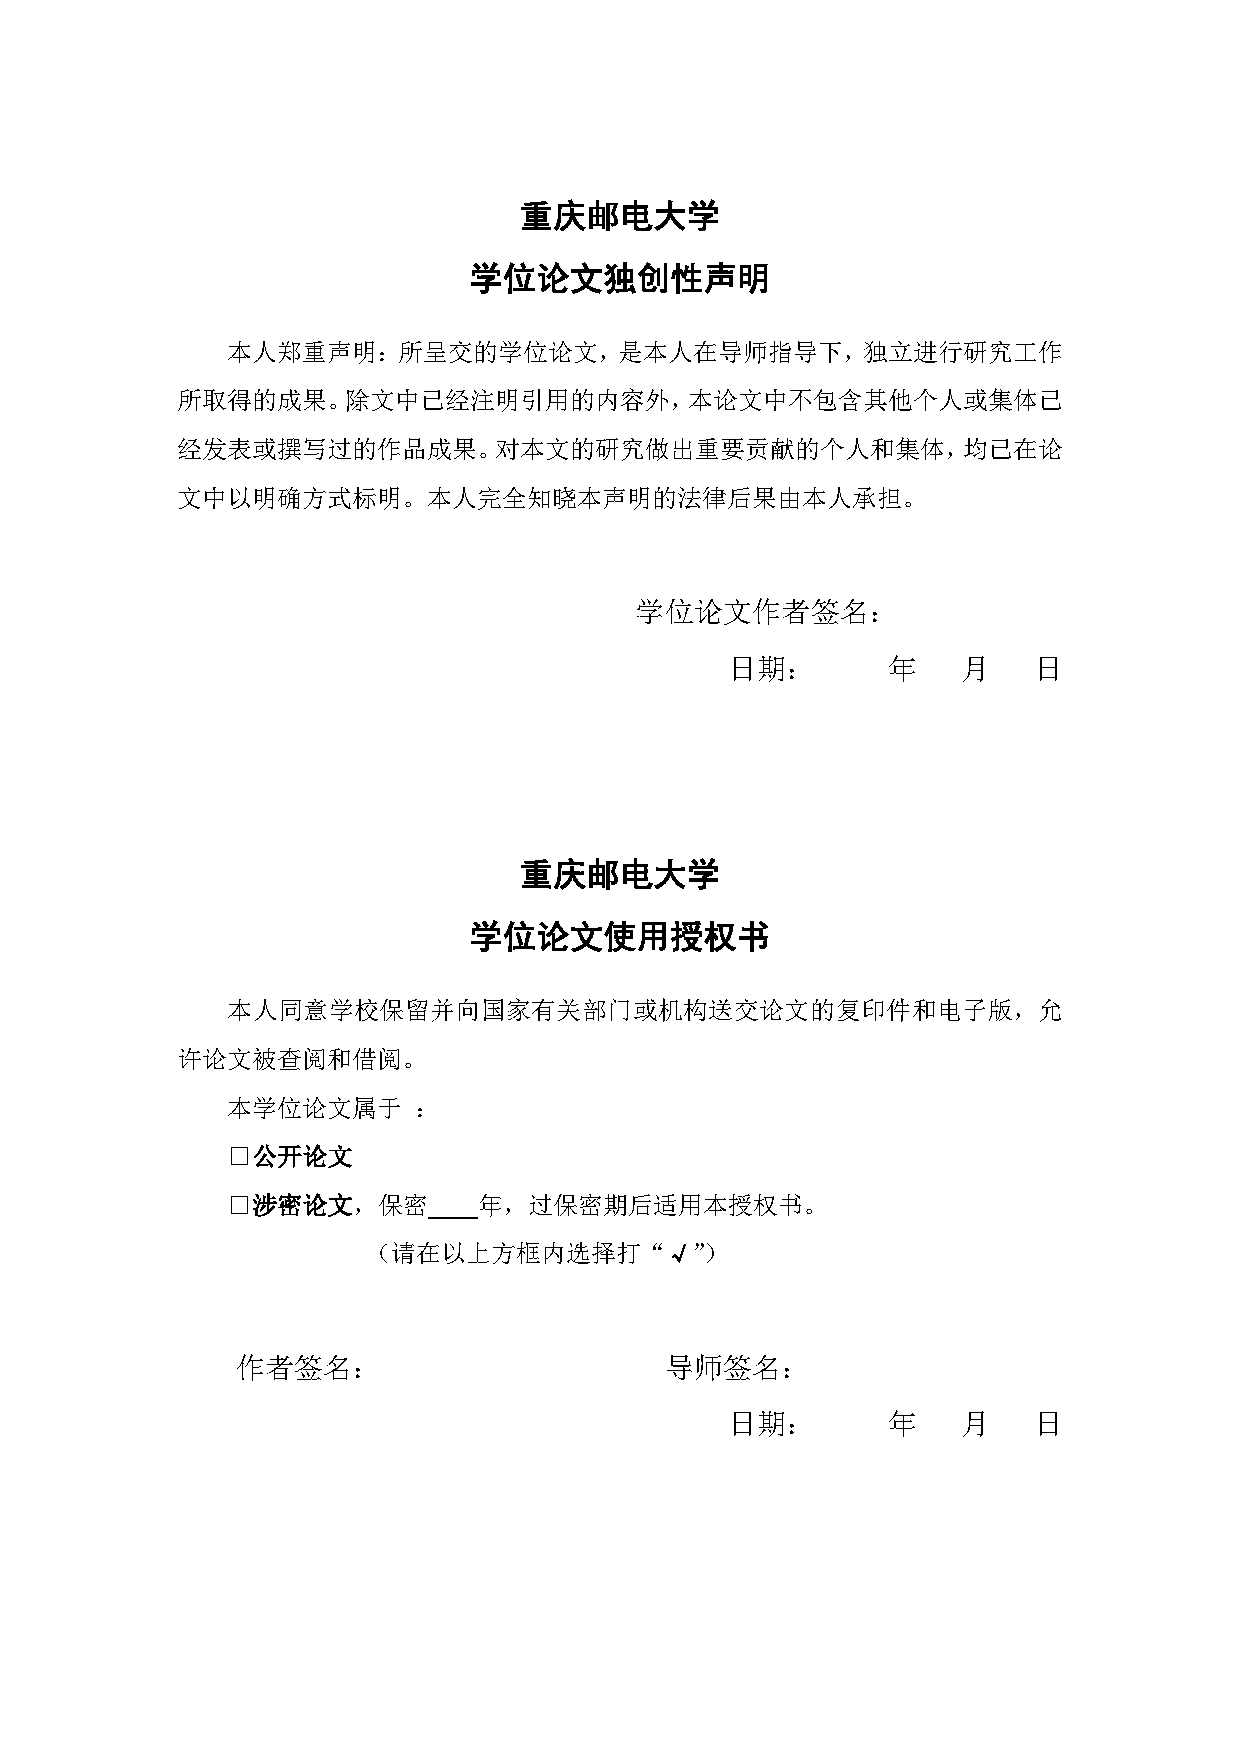
\includepdf{original.pdf}
\clearpage


\clearpage

%前序部分(中英文摘要,目录等,chapter后面不编号)
\frontmatter

%开始以大写罗马字母计页码
\pagenumbering{Roman}

\pagestyle{plain}
%页面格式
%\pagestyle{plain}

% 中文摘要页
%中文摘要,自行编辑内容

\chapter{摘 \quad 要}
\xiaosi
点云语义分割是三维场景理解的核心任务,其目标在于将场景中每个点准确地映射到预设的语义类别上,广泛应用于无人驾驶、智能机器人以及虚拟和增强现实等领域。随着深度学习技术的迅速发展,大规模点云数据的高效处理成为可能,并催生了大量优秀的开源模型。然而,尽管点云数据采集变得更加便捷,但全监督训练要求逐点标注的数据依然难以获取,因为大规模点云逐点标注是一项耗时耗力的工作。此外,由于不同采集设备和场景的差异,将源数据集上训练的模型直接应用于新目标数据集时常会出现显著的域间隙,从而导致性能下降。域自适应作为解决域间隙问题和减少对标注依赖的重要策略,目前主要采用无监督或半监督模式,虽然节省了标注成本,但往往会牺牲部分模型性能。相比之下,主动域自适应在人工成本与分割精度之间提供了更具性价比的平衡方式。然而,目前针对三维点云语义分割主动域适应尚未提出专门的主动查询策略,也缺乏将主动选择的目标域点与已标注的源域数据有效结合的方案。针对上述问题,本文对主动学习和域自适应在视觉语义分割中的研究进展和方法进行了归类总结,阐述了现有方法的优缺点。此外,进一步提出了有效的针对三维点云语义分割的域自适应的主动学习方法以及充分发挥两域潜能的主动混合方法,方法如下所示:

% 点云语义分割是三维场景理解中的一个关键任务,其旨在将点云场景中的每一个点都映射到预设的语义类别上。在无人驾驶、智能机器人、虚拟现实、增强现实等领域,点云语义分割都有着巨大的应用价值。得益于深度学习的蓬勃发展,大规模的点云数据处理变得简单而高效,涌现出一大批优秀开源模型。随着科技的进步,点云数据的获取也变得更加容易,但是这些直接获得的数据却无法直接应用到这些优秀的模型上去,因为这些模型都是在全监督模式下训练得到的,这要求点云数据必须是逐点标注的。而大规模点云逐点标注是一项耗时耗力的工作。并且由于传感器等一些设备参数的不同,直接将源数据集上训练的模型应用于新的目标数据集时,往往会出现显著的域间隙,导致模型性能下降。域自适应是解决域间隙和数据标注的方法之一。在三维点云语义分割中,域自适应主要以无监督和半监督模式为主,尽管能减少对标注的依赖,却也不可避免地牺牲部分模型性能。相比之下,主动域自适应在人工成本与分割精度之间提供了更具性价比的平衡方式。然而,目前针对三维点云语义分割尚未提出专门的主动查询策略,也缺乏将主动选择的目标域点与已标注的源域数据有效结合的方案。针对上述问题,本文对主动学习和域自适应在视觉语义分割中的研究进展和方法进行了归类总结,阐述了现有方法的优缺点。此外,进一步提出了有效的针对三维点云语义分割的域自适应的主动学习方法以及充分发挥域适应两个数据集潜能的结合方式,方法如下所示:

% 得益于深度学习的蓬勃发展,大规模的点云数据处理变得简单而高效,加之一些高质量的开源标注点云数据集的发布,为一些卓越模型的出现铺垫好了道路。然而,这些模型都是基于开源的标记的数据集进行训练的即全监督训练,对于点云语义分割任务来说,数据的标注是一项极其耗时耗力的工作,而面对复杂多变的实际场景,显然是不现实的。而如果直接将训练好的模型直接应用于新的数据集上,由于数据获取的设备和场景的不同会有域间隙的存在,这会导致在源数据集上训练好的模型性能将会下降。因此如何解决域间隙这一绕不开的问题自然而然成为一些研究者们的关注点。域自适应便是解决域间隙的一个主流策略。
% 对于三维点云语义分割任务,域自适应更多的是无监督、半监督模式下的,而这两种方式都与全监督有一点的差距,虽然节省了标签但同时也牺牲了性能,主动域自适应可以综合平衡人工花费和性能,是一种高性价比的方式,然而在三维点云语义分割领域并没有专门的主动查询策略被提出。并且没有将主动选择的目标点和有标记的源域数据有效的结合使用起来。针对上述问题,本文对主动学习和域自适应在视觉语义分割中的研究进展和方法进行了归类总结,阐述了现有方法的优缺点。此外,进一步提出了有效的针对三维点云语义分割的域自适应的主动学习方法以及充分发挥域适应两个数据集潜能的结合方式,方法如下所示:

1. 基于点云语义分割域适应的主动学习方法,其主要贡献如下:1)提出一种原型指导的域差异感知查询策略,通过计算目标域点云特征与源域类别原型中心的余弦距离,构建"特征距离-预测熵"联合评估指标,实现跨域场景下高迁移价值点的选择。2)首次将主动学习与混合方法进行结合并用于点云语义分割域适应任务,通过混合策略将主动学习选择的目标点与源域点进行混合,构建出强健的中间域数据,进一步缩减域间隙。
% 2)设计平衡式跨域混合增强机制,通过尺度感知的空间-语义对齐技术,将新标注目标域样本与源域数据进行语义级混合,有效解决主动学习过程中的域偏移累积问题。

2. 基于点云语义分割域适应的主动混合方法,其主要贡献如下:1)提出一种源-目标数量平衡算法,混合标注数量相同的源和目标域点,使得模型可以学到更加平衡的两域知识,解决模型学习过程中的域偏移累积问题。2)在源-目标数量平衡模块的基础上提出类别平衡主动混合算法,解决混合中间域类别不平衡问题,进一步提升模型的性能。

本文提出的方法在合成到真实,真实到真实的跨域任务上做了大量实验和验证。通过与现有的同类优秀域自适应方法进行对比,实验结果和可视化结果充分证明了方法的优越性,在极少数标签的情况下达到了超越全监督的效果。\\
% 本文提出的方法在多个用于点云语义分割域适应任务的主流室外数据集上进行了大量实验和验证,包括SemanticKITTI、SemanticPOSS、nuScenes、SynLiDAR,其实验场景涵盖了合成到真实,真实到真实的跨域任务。通过与现有的同类优秀域自适应方法进行对比,实验结果和可视化结果充分证明了方法的优越性,在极少数标签的情况下达到了超越全监督的效果。\\

% 学位论文是研究生从事科研工作的成果的主要表现,集中表明了作者在研究工作中获得的新发明、新理论或新见解,是研究生申请硕士或博士学位的重要依据,也是科研领域中的重要文献资料和社会的宝贵财富。
% 为进一步规范我校研究生学位论文撰写格式,提高研究生学位论文质量,参照国家标准《学位论文编写规则》(GB/T 7713.1-2006),结合我校实际,制定本模板。
\noindent\songti\textbf{关键词:}点云处理,三维视觉,语义分割,域适应,主动学习,混合方法

\clearpage


% 英文摘要页
%英文摘要,自行编辑内容




\chapter{ABSTRACT}
\xiaosi
% Point cloud semantic segmentation stands as a core task in 3D scene understanding, aiming to accurately map each point in a scene to predefined semantic categories. This technology finds widespread applications in autonomous driving, intelligent robotics, virtual reality, and augmented reality. The rapid development of deep learning has enabled efficient processing of large-scale point cloud data and facilitated the emergence of numerous high-performance open-source models. However, despite advancements in data acquisition, fully supervised training remains constrained by the labor-intensive nature of acquiring point-wise annotations, which are critical yet prohibitively costly to obtain at scale. Furthermore, models trained on source datasets often suffer significant performance degradation when deployed on new target datasets due to domain gaps caused by variations in data acquisition devices and environmental conditions. Domain adaptation has emerged as a pivotal strategy to mitigate domain shifts and reduce annotation dependency. Current approaches predominantly adopt unsupervised or semi-supervised paradigms, which reduce annotation costs but inevitably sacrifice segmentation accuracy. In contrast, active domain adaptation offers a cost-effective balance between human annotation efforts and model performance. Nevertheless, dedicated active query strategies for 3D point cloud semantic segmentation remain underdeveloped, and existing methods fail to effectively integrate actively selected target-domain points with labeled source-domain data.
% To address these challenges, this paper systematically reviews research progress and methodologies in active learning and domain adaptation for visual semantic segmentation, highlighting the limitations of existing approaches. We further propose two innovative solutions for 3D point cloud semantic segmentation, and the following methods are established:
Point cloud semantic segmentation is the core task of 3D scene understanding, and its goal is to accurately map each point in the scene to a preset semantic category, which is widely used in the fields of unmanned driving, intelligent robotics, and virtual and augmented reality. With the rapid development of deep learning technology, efficient processing of large-scale point cloud data has become possible and has given rise to a large number of excellent open-source models. However, although point cloud data acquisition has become more convenient, fully supervised training requiring point-by-point labeling is still difficult to obtain, because point-by-point labeling of large-scale point clouds is a time-consuming and labor-intensive task. In addition, due to the differences in different acquisition devices and scenarios, there are often significant domain gaps when directly applying models trained on source datasets to new target datasets, resulting in performance degradation. As an important strategy to solve the domain gap problem and reduce the dependence on annotation, domain adaptation currently mainly adopts unsupervised or semi-supervised modes, which saves the annotation cost but often sacrifices part of the model performance. In contrast, active domain adaptation provides a more cost-effective way to balance between labor cost and segmentation accuracy. However, no specialized active query strategy has yet been proposed for active domain adaptation for semantic segmentation of 3D point clouds, and there is a lack of schemes to effectively combine the actively selected target domain points with the annotated source domain data. To address the above issues, this paper categorizes and summarizes the research progress and methods of active learning and domain adaptation in visual semantic segmentation, and describes the advantages and disadvantages of the existing methods. In addition, effective domain-adaptive active learning methods for semantic segmentation of 3D point clouds as well as active mixing methods that fully utilize the potential of both domains are further proposed as shown below:

% 1. Domain discrepancy aware active learning for cross-domain segmentation. The main contributions are as follows: 1) We introduce a prototype-guided query strategy that computes the cosine distance between target point cloud features and source domain class prototypes. By integrating this distance with predictive entropy, we construct a joint evaluation metric that effectively selects high-transfer-value points in cross-domain scenarios. 2) We pioneer the combination of active learning with a mixing strategy in the context of domain adaptation for point cloud segmentation, blending actively selected target points with source domain data to create robust intermediate domain samples, thereby further reducing the domain gap.
1. A Domain discrepancy aware active learning for cross-domain segmentation, its main contributions are as follows: 1) The first prototype-guided domain discrepancy awareness query strategy, by calculating the cosine distance between the point cloud features of the target domain and the prototype centers of the source domain categories, and constructing a joint evaluation index of “feature distance-predictive entropy” to achieve the selection of points with high migration value in cross-domain scenarios. 2) For the first time, this paper combined the active learning with the mixing strategy and used it for the domain adaptation task of point cloud semantic segmentation, and constructed a robust intermediate domain data to further reduce the domain gap by mixing the target points selected by active learning with source domain points.

% 2. Active mixing method for cross-domain semantic segmentation. The main contributions are as follows: 1) We propose a source-target quantity balancing algorithm that ensures an equal number of annotated points from both domains are mixed, enabling the model to learn a more balanced representation and mitigating cumulative domain shift during training. 2) Building on this, we further introduce a category-balanced active mixing algorithm to address class imbalance in the mixed intermediate domain, which enhances overall model performance.
2. Active mixing method for cross-domain semantic segmentation, its main contributions are as follows: 1) Propose a source-target amount balance algorithm with the source-target amount balance algorithm, mixing the source and target domain points with the same number of labeling, so that the model can learn a more balanced knowledge of the two domains, and solving the problem of accumulating domain bias in the process of model learning. 2) Propose the class-balanced active mixing algorithm on the basis of the source-target quantity balance module, solving the mixing intermediate domain class imbalance problem and further improve the performance of the model.

% Extensive experiments on both synthetic-to-real and real-to-real cross-domain tasks demonstrate that our proposed methods outperform state-of-the-art domain adaptation approaches, achieving superior performance even under scenarios with extremely limited annotations.
The method proposed in this paper has been extensively experimented and validated on synthetic-to-real and real-to-real cross-domain tasks. The experimental and visualization results fully demonstrate the superiority of the method by comparing with similar existing excellent domain adaptive methods, even achieving results beyond full supervision in very few labeled cases.
% Dissertation /Thesis is postgraduate’s main academic performance to display her/his works of scientific research, which shows the author’s new invention, new theory or new opinion in her/his research. It is the crucial document for the graduate students to apply for degree, and it is also the important scientific research literature and the valuable wealth of society.
% In order to further standardize the format of dissertation/thesis writing and improve graduate dissertation/thesis quality, this temolate is formulated with reference to the national standard "Rules for Dissertation Writing" (GB/T 7713.1-2006) and the reality of CQUPT.

\noindent\textbf{Keywords:}Point Cloud Processing, 3D Vision, Semantic Segmentation,  Domain Adaptation, Active Learning, Mixing Methods

\clearpage


% 目录
%\begin{spacing}{1.14}
\tableofcontents


\begingroup
\renewcommand*{\addvspace}[1]{}
%图目录
%\newcommand{\loflabel}{图}
%\renewcommand{\numberline}[1]{\loflabel~#1\hspace*{1em}}
\listoffigures

%表目录
%\newcommand{\lotlabel}{表}
%\renewcommand{\numberline}[1]{\lotlabel~#1\hspace*{1em}}
\listoftables
\endgroup

%\end{spacing}


%主要符号表
% 

\chapter{主要符号表}



\begin{table}[h]
	\renewcommand{\arraystretch}{1.5}
	\centering
	\begin{tabular}{p{2cm}p{10cm}p{1.5cm}}
		\toprule[1.5pt]
		\makecell[l]{\songti\xiaosi\bfseries 符号}&\makecell[l]{\songti\xiaosi\bfseries 说明}&\makecell[c]{\songti\xiaosi\bfseries 页码}\\
		\hline
		\makecell[l]{\wuhao c}&\makecell[l]{\wuhao 电磁波的相平面速度}&\makecell[c]{\wuhao 10}\\
		\bottomrule[1.5pt]
	\end{tabular}
     
\end{table}

\clearpage

%缩略词表
% 



\chapter{缩略词表}

\begin{table}[h]
	\renewcommand{\arraystretch}{1.5}
	\centering
	\begin{tabular}{p{2cm}p{8.5cm}p{3cm}}
		\toprule[1.5pt]
		\makecell[l]{\songti\xiaosi\bfseries 英文缩写}&\makecell[l]{\songti\xiaosi\bfseries 英文全称}&\makecell[l]{\songti\xiaosi\bfseries 中文全称}\\
		\hline
		\makecell[l]{\wuhao CQUPT}&\makecell[l]{\wuhao Chongqing University of Posts Telecommunications}&\makecell[l]{\wuhao 重庆邮电大学}\\
		\bottomrule[1.5pt]
	\end{tabular}
	
\end{table}

\clearpage

\clearpage

%% 开始章节写作,chapter后面开始编号,显示特定页眉页脚
\mainmatter
\pagenumbering{arabic}

%正文页眉避免英文全部大写
\renewcommand\thechapter{\arabic{chapter}}
\renewcommand{\chaptermark}[1]{\markboth{第 \thechapter 章 \ #1}{}}

% 第1章
\chapter{绪论}
\thispagestyle{others}
\pagestyle{others}
\xiaosi

\section{研究背景及意义}
    随着科技进步和经济发展,人工智能已悄然融入人们的日常生活,智能产品正潜移默化地改变着生活方式、交通出行和娱乐方式。其中,无人驾驶\upcite{levinson2011towards}、机器人\upcite{zhou2022loop}以及增强现实\upcite{carmigniani2011augmented}等领域备受关注。这些技术的出现不仅使人们的生活更加便捷,出行更为高效,同时也丰富了娱乐体验。然而,在机器人和自动驾驶等应用中,环境感知能力是实现高级智能的核心,一个可靠的感知系统对于自动避障和环境识别至关重要。为确保实际应用中的安全性与准确性,优秀的感知系统往往需要集成多种传感器进行多模态数据采集,而激光雷达正是其中的一个关键传感器。激光雷达通过固定频率和角度发射激光,接收返回信号以采集周围环境信息,生成包含三维空间几何信息的点云数据,这一点是二维图像所无法提供的。此外,其采集的数据不受光照变化影响,能够真实还原物体的尺寸和形态,基于这些优势,激光雷达已被广泛应用于各种智能系统中。因此,如何高效利用三维点云数据实现精准感知,已成为当前非常重要的研究课题。
    点云语义分割是实现三维场景感知的关键任务。在无人驾驶和机器人领域,通过对周围环境和道路进行语义分割,可以为不同类别的点赋予相应的语义标签,从而将原始点云数据转化为含有语义信息的三维场景数据。基于此,系统能够依据环境中的语义标签有效区分不同物体,并据此调整导航路径,确保车辆或机器人的正确行进方向。在增强现实中,准确的语义分割则是实现虚拟内容与真实环境无缝融合的前提,只有对真实世界中的物体及其边界进行精确感知和分类,才能将虚拟场景合理地叠加到现实世界中,达到增强现实的效果。尽管点云语义分割的应用价值巨大,早在深度学习兴起之前便已引起学术界广泛关注,但受限于传统机器学习方法在处理大规模点云数据时的效率和性能不足,其研究进展较为缓慢。
    随着深度学习技术的发展,端到端的点云语义分割方法在大规模数据处理和分割精度上均取得了显著提升,为该领域注入了新的动力。大量优秀模型如雨后春笋般涌现。值得注意的是,由于点云数据集根据获取场景的不同又可以分为室内点云数据集\upcite{S3DIS,Scannet}和室外点云数据集\upcite{behley2019semantickitti,caesar2020nuscenes,pan2020semanticposs},它们各具特点。室内数据集密度均匀且规模相对较小,多用于增强现实和机器人等应用;而室外数据集则呈现近密远疏的特性,覆盖的场景更为广阔,通常用于无人驾驶等领域。尽管基于深度学习的算法在这两类数据集上均取得了显著进展,并为实际应用带来了美好前景,但这些算法普遍依赖于逐点标注数据进行全监督训练。然而实际上,一帧点云通常包含十多万个点,一个场景可能包含数千帧点云,而一个完整的数据集则可能涉及十多个不同场景。由于点云本质上是无序的几何数据,其标注工作需要专业人士操作,因此逐点标注不仅复杂而且极为耗时\upcite{behley2019semantickitti}。高昂的标注成本已成为制约这些先进算法落地应用的重要挑战。因此,如何在标注成本与模型性能之间取得平衡,以及如何利用已有数据或仅用少量标注数据训练出高性能的分割模型,成为亟待解决的关键问题。
    域适应作为解决上述问题的重要研究分支,其基本思路是利用已有逐点标注的全监督数据训练预训练模型,再将该模型迁移到未标注的目标域中,同时解决由于场景差异或传感器差异所引起的域偏移问题。常见的域适应方法包括无监督域适应、半监督域适应和主动域适应。无监督域适应虽然不依赖目标域标注,但其效果与全监督方法仍存在较大差距;半监督域适应虽然优于无监督方法,但由于目标域中标注数据通常为随机采样,受域偏移影响较大,其作用未能充分发挥。相比之下,主动域适应通过结合主动学习方法,从目标域中选择对模型迁移最有价值的样本进行标注,既有效缩小域间隙、提升了模型性能又降低了标注成本。然而,目前基于语义分割的主动域适应研究主要集中在二维图像领域,而在三维点云领域尚缺乏系统性的探索。此外,传统的主动学习方法难以直接应用于域适应场景;同时,由于主动学习选择的样本数量较少,如何充分利用源域和目标域的标注数据,既发挥各自潜力又有效防止域偏移累积,仍是需要解决的问题。因此,本文的研究以主动学习和域适应为出发点,首先通过大量文献调研,基于域适应的特点寻找适用于三维点云语义分割任务的主动查询策略;随后,深入探索主动标注样本与源域数据的有效融合及主动学习混合策略,以期获得更加稳固的跨域特征表示。最后,通过大量实验对提出方法进行验证分析。

\section{国内外研究现状}
本文主要研究方向为点云语义分割任务下的主动域适应,因此重点是探索适合点云语义分割域适应任务的主动学习方法,并在此基础上进一步研究适合主动学习的混合(Mixing)方法,因此相关工作涉及到点云语义分割、主动学习、域适应以及Mixing数据增强等相关领域。所以本节将分别对这四个领域中最近几年的相关研究和进展进行分析和总结。
\subsection{基于深度学习的点云语义分割方法}
由于传统机器学习方法难以高效且精确地对大规模点云数据实现逐点分割,基于端到端的深度学习方法因其大批量数据处理能力已成为点云语义分割任务的主流方法。这些方法大致可以分为三类:基于二维投影的点云语义分割方法、基于体素的点云语义分割方法和基于点的点云语义分割方法。
基于二维投影的方法通过不同的投影视角将无序非结构化的点云投影到结构化的二维图像中,投影方法包括鸟瞰图\upcite{aksoy2020salsanet},球形\upcite{cortinhal2020salsanext,RangeNet++,wu2018squeezeseg,wu2019squeezesegv2,xu2020squeezesegv3},多视角\upcite{boulch2017unstructured,kundu2020virtual}等。然后利用更加成熟稳定的二维卷积网络去对这些点云图片进行特征提取和语义分割,并将分割后的结果映射回点云中。此类方法的核心思想是模态转变,将点云从三维转变为图像,然后就可以利用二维卷积网络处理。但是其不足也非常的明显,二维和三模态差异导致其表征信息的方式也有所不同,模态的转换导致三维几何信息被破坏,进而造成信息的丢失。因此,完全基于投影的方法在随后的研究中,逐渐被人遗忘,研究者们转而开始寻找更加有效的点云语义分割的处理方式。有研究者认为图像模态下的点云可以提取不同于三维模态下的特征,为了充分利用图像提取到的信息,提出了混合点云三维特征和二维特征的多模态方法,这种方法将两者的处理结果相结合,形成了优势互补\upcite{robert2022learning,wang1022567052},并成功取得非常可观的分割效果。
基于体素的方法首先将三维点云数据转换为体素网格,即将原本离散且稀疏的点云数据规整成规则的三维格状结构,接着利用稀疏卷积技术在该结构上进行特征提取和表示学习,从而获得较为紧凑且具有表达能力的点云特征。这种方法在处理大规模室外场景时表现出较高的效率,因为规则化的体素结构便于卷积操作的实现,并可显著降低计算复杂度。然而,体素化过程中由于数据离散化的固有属性,往往会导致细节信息的损失,尤其是在高分辨率特征提取方面存在一定局限。这些方法中有一些是比较优秀且至今仍被作为基础框架研究的。MinkowskiNet\upcite{MinkowskiNet}提出了一种高可用到的稀疏卷积方法,并构建了一个专门用于稀疏张量的自动微分库。基于这一方法与工具,构建出一种四维卷积神经网络,用于时空感知任务,其设计能够同时捕捉空间与时间维度的信息,实现更为精准的特征提取。而之后提出的一些稀疏卷积方法\upcite{graham20183d,tang2020searching}则是对许多无意义的计算消耗进行了改进,进一步提高了计算效率。最新的基于体素的方法OA-CNNs\upcite{peng2024oa}则提出了一种全自适应三维卷积神经网络,该网络由动态感受野和自适应关系映射组成:空间动态感受野能够根据输入数据的分布灵活调整感受区域;自适应关系卷积,用于捕捉并建模局部特征之间的复杂关联。因此其在一定程度上展现了超越Transformer架构的潜能。由于点到体素的转换,一定程度上缓解了计算消耗,因此这些方法更适用于大规模的室外点云场景处理。
基于点的方法直接将点云输入到分割网络而不进行任何处理。在提出PointNet\upcite{PointNet}架构之前,三维点云特征的提取都是手动完成的。PointNet是第一个能够直接使用三维点云提取深度学习特征的架构。其通过提取点云特征中的最大值来处理点云的无序特性,然而这也会导致其无法利用点云中的局部结构信息,无法运用到大规模数据集上。而它的改进版本PointNet++\upcite{PointNet++}的主要贡献在于提出了分层结构,使用多个抽象层进行特征提取, 从而实现邻域局部特征和全局特征的提取。受PointNet的影响和启发,更多的基于点的方法\upcite{KPConv,li2018pointcnn,wu2019pointconv}被提出。其中,KPCov\upcite{wu2019pointconv}提出了一种新型点卷积算法,其利用一组核点来确定卷积核权重的作用区域,从而在保留点云完整几何信息的同时克服了传统点卷积的局限性。该方法借鉴了图像卷积的思想,但通过灵活定义核点的数量和位置,实现了对局部特征的高效提取,并以相关函数确定其影响范围。采用半径邻域和规则下采样策略,有效应对了非均匀采样问题,从而在大规模点云场景下保持较高鲁棒性和计算效率。此后,RandLA-Net\upcite{hu2020randla}引入了一个局部特征聚合模块,有效地保留来自大范围邻域的有用特征,并在其方法中使用随机采样,以显著减少内存占用和计算成本。SCF-Net\upcite{fan2021scf}提出了一个可学习的SCF(Spatial Contextual Features)模块,由三个部分组成:局部极坐标表示模块(LPR)、双重距离注意力池化模块(DDAP)和全局上下文特征模块(GCF)。LPR模块在极坐标系中构建z轴旋转不变的表示,以捕捉每个3D点的局部上下文。DDAP模块通过利用几何距离和特征距离学习的权重,整合邻域点的表示,学习有效的局部特征。GCF模块利用邻域的位置和体积比,学习每个3D点的全局上下文。SCF模块可以嵌入到各种网络架构中用于点云分割,但其网络结构比较复杂。BBAF-Net\upcite{qiu2021semantic}通过引入密集区域来增强局部上下文解决相邻点的模糊性,同时自适应地融合多分辨率特征,以获取关于点云的全面知识。而随着注意力机制下大模型的爆火,Transformer\upcite{zhao2021point}首次将注意力机应用到点云语义分割任务中。随后的一些工作也将其加入到自己的方法中\upcite{JSJF202203012,GXJM202207010},虽然注意力机制完美适配了点云的无序特性,然而这些方法大多需要更多的计算时间。TransformerV3\upcite{wu2024point}探索了一种新的序列化邻域机制,将点云按照特定模式组织起来。并采用简化方法取代了更复杂的注意力区域交互机制,从而更适用于序列化点云处理。同时消除了对相对位置编码的依赖,并采用了一种更简单的前置稀疏卷积层进行特征提取,从而提高计算效率。基于点的方法能够完整保留点云中每个点的原始几何信息和局部特征,这一优势使其在三维语义分割任务中展现出独特的潜能。当前虽已有不少相关方法取得了显著进展,但在深层次特征利用以及复杂场景的细粒度信息捕捉方面,仍存在大量未被充分挖掘的可能性。随着计算机视觉与深度学习技术的不断演进,未来在这一领域内定将涌现出更多创新方法,为三维数据的高效处理和精准理解提供更加完善的解决方案。
虽然上述算法都在基于深度学习的点云语义分割任务中取得了优异的结果,但是这些方法仍然需要基于全标注的数据进行训练才能实现最佳的效果,而对于点云语义分割任务来说,逐点标注是极其复杂的一项工程。如何平衡性能与标注是一个非常重要的研究方向,主动域适应是其中一个方法, 也正是本文的研究目的所在。

\subsection{视觉语义分割中的主动学习方法}
随着深度学习的发展,模型高性能与数据标注困难以及无标注但性能低的问题也逐渐显现,因此一些研究者开始将目光转向能够平衡性能与标注花费的主动学习上来。在视觉语义分割任务中,根据其筛选的基本单元的不同,大致可以将其分为基于样本的主动学习方法, 基于区域的主动学习方法和基于最小语义单元的主动学习方法。
\subsubsection{基于样本的主动学习方法}
在主动学习的早期阶段,研究者们主要采用以样本为基本查询单位的方法。这一策略源于主动学习最初在视觉分类任务中的应用,而在这些任务中,数据通常是以单个样本为单位进行划分和标注的。因此,许多针对语义分割任务的早期方法也从分类任务中获得了启发,采用在每一轮数据选择中筛选出信息量丰富的样本并进行逐点或者逐像素的标注。Tan等人\upcite{tan2019batch}的研究重点在于充分挖掘类别的边缘信息。他们提出了一种方法,首先借助边缘检测器提取图像中的边缘特征,然后将这些边缘信息与利用KL散度评估的不确定性及数据代表性相融合,以实现主动样本选择。该方法将传统的人工设计理念与任务的实际需求紧密结合,取得了显著成效。Sinha等人\upcite{sinha2019variational}出了一种新的池化主动学习算法,该算法基于变分自编码器(VAE)和对抗网络,通过隐式学习采样机制来选择最具代表性的查询样本进行标注,从而提高模型性能并降低标注成本。Zhang等人\upcite{zhang2020state}提出了一种状态重新标记对抗性主动学习模型,模型充分利用标注信息和状态信息,用于推导出对于当前模型来说信息最丰富未的标记样本。其设计了一种在线不确定性指示器,重新标记未标记数据的状态,赋予其不同的重要性,同时构建了一个无监督的图像重建器和一个监督的目标学习器,生成图像的统一表示,迭代嵌入标注信息。最后结合所提出的k-center方法的初始采样算法,使后续采样更加高效。但这些方法通常以全局不确定性或多样性为准则筛选样本,忽略了语义分割任务中不同区域的内在难度差异,导致标注资源浪费且模型在困难区域表现不足。为了解决这问题, Xie等人\upcite{xie2020deal}提出了难度感知的主动学习方法DEAL。该方法通过引入语义难度分支和设计像素级概率注意力模块动态学习不同语义区域的难度分数,并利用分割误差作为监督信号,使模型准确捕捉那些易混淆或低置信度的像素区域,从而将主动学习的焦点从整体信息量转向局部难度感知。为了解决困难区域样本稀缺的问题,该方法进一步提出了一种双阶段样本获取策略,基于语义难度分数筛选出包含高难度区域的图像,并结合区域不确定性和多样性对像素级标注进行优先级排序,实现了从图像级粗筛选到像素级细粒度标注的渐进式优化。Huang等人\upcite{huang2021semi}利用一种新颖的无标签数据采样策略,结合半监督训练方案进行数据注释,从而利用无标签数据提升任务模型的性能。
基于样本的主动学习方法虽然能够降低标注成本,但在视觉语义分割任务中也存在一些不足。由于一幅图像往往包含多个类别,而各类别的区域大小和分布差异明显,所选样本中的大部分信息可能仅集中在部分类别,其他区域则容易成为噪声。而且标注过程中常见的类别不平衡问题可能导致模型在训练时偏重于主流类别,从而忽略细节部分。此外,语义分割需要对每个像素或者点进行精细判断,单纯依赖样本级的选择往往难以捕捉到局部的复杂信息,这在处理复杂语义区域时尤为明显。
\subsubsection{基于区域的主动学习方法}
在语义分割任务中,基于样本的主动学习方法问题逐渐显现,一些研究者开始寻找缓解问题的方法。由于不同的区域对样本的影响程度不同,因此基于区域的主动学习方法被提出,这种方法将样本划分为不同的区域并作为查询和标注的基本单元。Qiao等人\upcite{qiao2022cpral}提出了一种基于区域的主动学习方法框架CRPA,通过结合全景和区域信息选择策略,有效平衡了标注工作量和模型性能。该框架引入了区域高斯注意力模块来缓解类别不平衡问题,并通过上下文标签扩展模块区域标注,进一步提高了标注效率。但是这种方法的划分是基于规则区域的,即将图像规则划分为同等大小的区域,然而语义类别在图像上的分布往往是不规则的,因此规则区域虽然有效降低了标注成本,却依然存在区域内类别不平衡或者分布不均匀的问题,导致少量的语义类别学习困难。Siddiqui等人\upcite{siddiqui2020viewal}提出了一种基于不规则区域面向深度图像的主动学习方法。其设计了一种基于KL散度的最优视角选择标准,用于衡量预测概率分布在不同视角之间的变化。通过分析预测在不同视角下的不一致性来估计模型的不确定性,并将其定义为视角熵。最后将视角熵与超像素区域选择相结合,使得模型能够高效地筛选出高价值的样本区域。针对普通图像,Cai等人\upcite{cai2021revisiting}也提出了一种类别平衡的采样策略,以提升超像素方法的性能,该策略能够优先选择来自低占比类别的高信息量样本。方法通过计算每个区域的最小边际不确定性,再依据每个区域主导类别所占比例对不确定性进行调整,从而获得更精准的不确定性度量。同时该文章也通过一系列的实验证明了不规则超像素在降低标注成本方面优于规则化的区域。
而在三维点云语义分割的主动学习方法中,区域的划分根据点云的非结构化几何特征而呈现出多样性。Lin等人\upcite{lin2020active}提出了一种主动增量学习框架,通过迭代地选择高信息量样本,逐步丰富模型知识,从而有效降低标注需求。该方法将点云数据被划分为多个小块,并分为已标注和未标注两组。已标注的小块用于训练,在初始迭代中,网络从零开始训练。在后续迭代中,采用微调策略,使模型在已有知识的基础上不断扩展。每轮训练完成后,网络会根据点熵、分割熵和互信息评估未标注点云小块的信息量,并选择最具信息价值的小块进行标注。Wang等人\upcite{wang2023one}提出了一种结合准场景级弱标签的主动弱监督框架,用具有固定半径的球形子点云作为查询单位,每个子点云类别仅需一个点级标签,通过主动策略识别并选择最具信息量的子点云进行标注,从而同时兼顾场景级和点级语义信息。Xie等人\upcite{Annotator}则是将点云划分到同等大小的体素网格中,然后对网格中的点的类别进行预测,计算其内部类别点的熵程度,值越高说明体素网格中包含的不同的类别的点越多,体素网格中的点类别分布越平衡,包含信息越丰富。除了上述规则的方式以外,其实更多的则是通过不规则区域即超点的形式进行的区域划分。Shao等人\upcite{shao2022active}提出了一种结合类平衡不确定性和多样性采样策略。该策略引入加权超点不确定性估计,根据超点中的多数类和少数类点赋予不同权重,以更准确地衡量超点的不确定性。同时,通过空间结构多样性推理机制,构建出超点图和图聚合操作,将超点特征投影到多样性空间中,利用最远点采样选择最具代表性的超点进行标注。Hu等人\upcite{hu2022lidal}提出了一种新颖的基于视角一致性的不确定性度量方法,以利用帧间约束信息。该方法基于连续 LiDAR帧中预测分数函数的方差,设计了新的帧间散度和熵公式,对于一个未标注目标,如果其预测标签在不同帧之间存在较大差异,便认为模型预测不可靠,并选择这些最具不确定性的区域进行人工标注。与Hu利用时序帧间一致性的思路不同,Liu等人\upcite{liu2024active}提出了一种基于多版本预测一致性的主动学习策略,通过数据增强构建输入点云的多个变体,以评估模型预测的稳定性。针对每个点在不同增强版本中的预测结果,计算其对应最高置信度类别的概率分布标准差作为不确定性度量,为缺乏连续帧数据的场景下提供了更灵活的标注策略。而Wei等人\upcite{wei2024basal}则提出了一种基于尺寸平衡的主动学习方法,旨在解决点云语义分割中的类别不平衡与冷启动问题。该方法主要通过物体尺寸特征间接平衡类别分布,将不同尺寸的物体聚类为同一类别,在选择的时候优先选择各类别分区中息量最大的簇进行标注。基于区域的方法由于在标注和性能上都有所突破,因此仍是语义分割任务中比较主流的方法。
\subsubsection{基于最小语义单元的主动学习方法}
语义分割任务中基于区域的主动学习方法显著优于基于样本主动学习的方法。为进一步优化标注效率,部分学者提出将选择粒度细化至最小语义单元,旨在通过精准标注关键局部区域,实现以更低成本的更高表现。在二维图像中,最小的语义单元是像素,因此在面向图像的基于最小语义单元的主动学习方法中,都是以像素为基本选择和标注单位。Shin等人\upcite{shin2021all}提出了第一个基于像素的主动学习框架,该方法将基于边界的不确定性策略运用到了不同的图片像素间,并比较不同像素间的差异最为衡量指标。该方法证明了仅在少量像素点上提供标注的情况下,深度神经网络能否依然取得良好表现,并证明在语义单元层面的标注,模型仍然能够有效学习语义信息。Rückin等人\upcite{ruckin2024semi}则是进一步将基于像素的主动学习方法与半监督学习相结合,并运用到了实际场景中。这一举措从实际运用层面证明了基于像素的主动学习标注的有效性和和高效性。而在三维点云语义分割中,最小语义单元是点。Xu等人\upcite{xu2023hierarchical}提出了第一个基于点的主动学习方法,该方通过加权计算每个点与不同层次下周围领域信息的熵值总和,然后选择出不确定性排名靠前的点,同时通过一种特征距离抑制的方法来过滤空间距离相近且类别相似的冗余点。该方法不仅提高了模型性能,也大大增加了有效标注率。以上这些主动学习方法不仅显著降低了所需的标注比例,还能在保持模型性能达到全监督水平约90\%的前提下,大幅降低人力成本。但是,传统的主动学习方法主要适用于单一数据集,对于存在显著域间差异的域适应任务则难以直接应用。
\subsection{视觉语义分割域自适应方法}
殊途同归,与主动学习不同的是域自适应方法则通过模型迁移的方式来解决目标域数据需要大量标注的问题。其核心思想是将在有标注的数据上训练好的模型迁移到无标注的目标域上去,并解决因域偏差而导致的模型性能下降问题。基于视觉语义分割的域自适应方法大致可以分为三类:无监督域自适应方法、半监督域自适应方法以及主动域自适应方法。
\subsubsection{无监督域适应}
目前,在三维点云领域,研究者们更多地关注基于无监督的域自适应方法。当聚焦于点云语义分割任务时,根据跨域数据集的差异,这些方法又可以分为两类:真实到真实的场景,以及合成到真实的场景。真实到真实的无监督域自适应方法,通过使用LiDAR传感器捕获的真实场景数据进行深度网络训练,随后在不同LiDAR传感器捕获的未知场景中进行测试。在这种情况下,Yi等人\upcite{yi2021complete}将域适应形式化为3D表面补全任务,该方法通过设计并训练一个上采样网络,将雷达线束补全到统一的64线,然后再将补全后的数据输入到分割模型进行分割。而Langer等人\upcite{langer2020domain}则通过射线投射将目标域的传感器模式转移到源域。在合成到真实的域自适应中,源数据通过模拟LiDAR传感器获得非真实场景的合成数据,而目标数据则由真实LiDAR传感器采集。在这种情况下,域偏移是由于采样噪声、环境结构和类别分布的差异引起的。Wu等人\upcite{wu2018squeezeseg}认为注意力模型可以用于聚合上下文信息,并且可以采用逐步域校准的测地线相关对齐来改善域自适应。在后续的文章中,Wu等人\upcite{wu2019squeezesegv2}则是通过生成对抗网络在合成数据上模拟真实的点云噪声。类似地,Xiao等人\upcite{xiao2022transfer}将域偏移分解为外观差异和稀疏度差异,然后应用生成网络来减轻每个差异。Saltori等人\upcite{saltori2022cosmix}则是通过对源域和目标域分别进行语义选择而后进行混合再放入到师生模型中进行训练,从而提高模型的性能。Ding等人\upcite{ding2022doda}提出了一个可以运用在室内数据集上的方法,其注意到了长尾类问题,设计了一个长尾类别注意机制,把已经打好伪标签的目标域长尾类别数据和源域进行混合后一同放入模型中训练。Bian等人\upcite{bian2022unsupervised}提出了一个基于图的框架来探索两个域之间的局部级特征对齐,在两个域上动态构建局部特征图,并利用源域的图建立记忆库,使用最优传输来生成图匹配对,最后基于图的局部特征损失来调整两个域之间的特征分布。Jiang等人\upcite{jiang2021lidarnet}设计了一个可以提取领域共享特征和领域私有特征的模型,然后利用GatedSCNN网络使领域共享特征提取器能够在领域共享特征中保留边界信息,并利用学习到的边界来完善分割结果。然而这些方法与在全监督下测得的目标数据集的性能上界仍存在很大的差异。
\subsubsection{半监督域适应}
为了解决无监督域适应与全监督性能差距过大问题,一些学者提出了基于半监督以及弱监督的域适应方法,但是这些方法目前在三维点云中出现的并不多,尤其是在三维语义分割领域中。Jaritz等人\upcite{jaritz2022cross}提出了第一篇点云语义分割领域的半监督域自适应。其使用跨模态的方式进行学习,利用点云几何先验信息以及图像的纹理颜色信息,并取二者的优点进行互补,使得提取的特征更加鲁棒,其具体实现是设计了一个双流、双头架构,一端是图像输入,一端是点云输入,在三维语义分割任务中对图像和点云模态应用了跨模态损失。跨模态损失包括应用于两种模态预测之间的KL散度,从而加强一致性。Chen等人\upcite{chen2021semi}提出了双层面域混合架构,从样本和区域层面混合两个域,生成两个老师模型,并通过这两个老师模型蒸馏知识给一个学生模型,使得学生模型更加强大,而其生成的伪标签将继续用于下一次双域混合中训练老师模型。Saito等人\upcite{saito2019semi}提出了一个由特征编码网络组成模型,使用一个分类层,用来计算特征与一组估计类别代表的相似性。通过交替地最大化未标记目标数据相对于分类器的条件熵和最小化其相对于特征编码器的条件熵来实现自适应。Yu等人\upcite{yu2023semi}则是从数据的角度来看问题,认为原始源标签可能存在噪声,因此将域自适应作为一个噪声标签学习问题,并利用具有伪中心的质子集的预测来修正源标签。Saltori等人\upcite{saltori2023compositional}设计了一种双分支对称网络架构,能够同时处理来自源域和目标域的点云,并通过跨域语义混合来减少域间分布差异。该方法基于教师-学生框架,在源域和目标域之间混合点云片段,然后利用源标签和目标伪标签进行监督,同时结合少量人工标注数据进一步提升性能。尽管在少量真实标注的支持下,半监督域自适应方法相较于无监督方法已经取得了显著的性能提升,但与目标域下全监督的结果仍存在一定差距。同时,半监督方法中所采用的标注往往具有较大的随机性,无法确保每个标注点都能有效地促进模型性能提升,这在一定程度上暴露了标注效率的问题。
\subsubsection{主动域适应}
基于半监督和弱监督的方法在一定程度上提升了模型性能,但其标注点的选取往往是随机进行的,这使得数据利用效率和标注效果存在一定局限。为实现更高效的标注并充分挖掘数据的潜在价值,部分学者开始探索将主动学习与域适应技术相融合,通过主动学习策略在目标域中主动选取那些信息量大、价值高的点,而非被动地随机标注低价值数据,同时利用域适应技术最大化这些数据的效用。然而,传统主动学习策略通常依赖于模型对数据的筛选,而在域适应场景中,模型往往基于源域数据进行训练,由于存在域间隙,这种筛选过程可能导致所选标注点失效,最终引发无效标注的问题。早期的主动域适应研究提出通过利用对抗训练的领域判别器来衡量每个目标实例的不确定性和域特性。不同于之前的方法,CLUE\upcite{CLUE}则提出了一种熵加权聚类算法,用于查询目标域中不确定和多样化的样本。而SDM\upcite{SDM}被提出来优化边际损失函数,以探索与源领域中潜在硬样本相似的目标实例。然而,现有的主动域适应方法大多刻意设计手工制作的查询函数来评估样本的注释值,并对所有目标数据一视同仁地采用相同的适应策略。这种僵化的标准使它们很容易过度适应某些领域的适应情况,从而限制了主动域适应方法的泛化。一些具有创新性的主动域适应方法,类似Huang等人\upcite{Divide}采取了分而自治的思想,把目标域上的数据分为4类,分别对这类数据进行不同的定制学习,但是这个方法是用在分类任务上的对于语义分割来说难以直接利用。MHPL\upcite{HPML}发现满足邻近混沌区域、个体差异和来源不相似属性的样本是信息量最大的样本,并将其定义为最小快乐点,并设计了最小快乐点学习方法(Minimum Happy Point Learning, MHPL)以很好地探索和利用最小快乐点,有效提高模型性能。Annotator\upcite{Annotator}是首个将主动域适应方法应用于点云语义分割任务的方案。该方法将点划分至更大的体素块中,并采用专门设计的体素混淆度选择策略,在有限预算下实现了高效的样本选择与性能优化。然而,其主动学习策略并非专门为域适应场景设计,类似于传统主动学习方法,仍忽略了域差异可能导致所选样本在目标域上无法实现最佳提升的问题。

\subsection{视觉语义分割中的Mixng方法}
Mxing方法在深度学习中,一直被作为一种数据增强的方式进行使用。其核心思想是通过混合不同的样本或特征来增强模型的泛化能力和鲁棒性,然而不同的任务和模态下的数据其Mixing的方式也有所不同。
2018年,Zhang等人\upcite{zhang2017mixup}首次提出mixup方法,用于超越经验风险最小化。这是第一篇关于mixing的文章,其通过线性插值的方式将训练样本及其对应的标签进行凸组合,将组合后的数据用以训练模型,从而正则化神经网络,使其在训练样本之间表现出更简单的线性行为。该方法被用于分类任务上,并显著提高了模型的泛化能力,其在面对对抗样本和标签噪声时表现出很强的鲁棒性。然而,mixup在图像分类任务中虽然表现优异,但在语义分割这种需要细粒度分类的任务中存在局限性。为了解决这一问题,CutMix方法\upcite{yun2019cutmi}被提出。该方法通过切割和粘贴图像区域,结合标签的线性插值,不仅保留了mixup的正则化效果,还能够更好地处理局部特征,从而在弱监督目标定位和图像分类任务中取得了更好的性能。随着研究的深入,Mixing方法逐渐被应用到三维点云数据处理领域。Mix3D方法\upcite{nekrasov2021mix3d}首次被提出,并用于3D场景的上下文数据增强。其通过混合两个增强场景,将对象实例隐式地放置在新的上下文中,从而帮助模型减少对场景上下文的依赖,更多地关注局部结构和特征。为了进一步提升模型在不同领域数据上的适应能力,CoSMix方法\upcite{saltori2022cosmix}被提出,用于3D点云分割的领域自适应。该方法通过组合语义信息和几何信息的样本混合策略,有效地平衡了全局上下文和局部几何结构,从而在不同领域数据上取得了更好的性能。随后,LaserMix方法\upcite{kong2023lasermix}被提出,用于半监督的LiDAR语义分割任务。该方法通过混合来自不同LiDAR扫描的激光束,鼓励模型在混合前后做出一致且正确的预测。该方法在多个主流LiDAR分割数据集上展示了其有效性和优越性。
尽管这些Mixing方法在解决特定问题上展现了卓越的性能提升,但目前它们主要与无监督、半监督乃至弱监督策略相结合,而在主动学习领域的应用仍未得到充分探索,而这正是本文关注和研究的重点之一。

\section{论文研究主要内容}
本研究聚焦于三维点云语义主动域适应问题,旨在探索和设计一种主动学习方法,以选择出对模型迁移最具价值的目标样本。同时,为了充分挖掘源域数据和主动标注样本的潜能,本文设计了一种高效的数据混合策略,将两者有机结合,从而进一步提升模型性能。主要研究内容如下:
1)大量查阅相关领域文献,对基于深度学习的点云语义分割算法、视觉语义分割中的主动学习方法以及域自适应技术的最新进展及存在问题进行了系统梳理。通过总结上述研究成果,本文阐明了现有方法的优势与不足,并探讨了可改进的方向,为新方法的提出提供了坚实的理论基础。
2)提出了基于点云语义分割域适应的主动学习方法。该方法由三个模块构成:源域原型构建模块、源域原型指导的数据选择模块和动态混合中间域构建模块。首先通过动态构建源域原型来代表源域类别质心,并在每一轮主动学习阶段实时更新原型,在进行目标域候选点筛选时,计算每个目标域中未标注的点与每个源域类别原型的相似度,通过最优-次优差异算法获取归一化后的类别概率的差值得到域差异性评分,同时结合不确定性评分得到最终候选评分,升序排列后选取前 k 个同时兼备高不确定性和高域差异性的目标点。此外,该方法首次将主动学习方法与混合(Mixing)策略结合,构建包含目标域信息和源域信息的中间域数据,帮助模型学习到更稳定的域不变特征,进一步缩小域间隙
3)提出了深度结合主动学习与混合策略的主动混合方法。该方法在基于点云语义分割域适应的主动学习框架上进行了深入探索,旨在解决由于数据量问题导致的域偏移累积以及主动学习选点不平衡问题。具体而言,该方法将动态混合中间域构建模块细分为两个模块:源-目标数量平衡模块和类别平衡主动混合模块。在每一轮主动学习过程中,通过动态匹配源域与目标域标注点的数量,确保混合数据中双域信息的均衡融合;同时,类别平衡主动混合模块保证了混合后数据的类别分布相对平衡,从而增强了主动学习与混合策略之间的协同作用。

\section{论文组织结构}
本文一共分为五个章节,各章节安排如下:
第1章为绪言,本章主要针对点云分割的研究背景、意义以及国内外的现状做详细阐述。首先介绍点云语义分割主动域适应方法的研究背景和研究意义。其次分别介绍了基于深度学习的点云语义分割方法、视觉语义分割相关的主动学习方法和域自适应方法以及视觉语义分割中的混合方法(Mixing)。最后简述本文的主要研究内容以及论文的主要组织架构。

第2章对点云语义分割,主动学习及域自适应等本文研究涉及领域的基础知识做详细阐述。首先介绍了点云表示及点云语义分割模型基础,并介绍了点云语义分割中的常用评价指标;接着介绍了主动学习的相关基础概念和流程;随后又介绍了域自适应的基础概念和常用域对齐方法;最后对跨域点云语义分割任务中常用的主流公开数据集进行了介绍。

第3章提出基于点的主动半监督点云语义分割方法。首先介绍了该方法的研究动机和贡献,接着详细的阐述了提出的方法框架和基于原型指导的学习方法,包括动态源域原型构建模块、原型指导的数据选择模块和动态中间域构建模块,最后在合成到真实(SynLiDAR$\to$SemanticPOSS、SynLiDAR$\to$SemanticKITTI)以及真实到真实(SemanticKITTI$\to$nuScenes、nuScenes$\to$SemanticKITTI)的跨域场景下进行了大量实验验证以及可视化分析证明该方法的有效性。

第4章提出基于点云语义分割域适应的主动混合策略。同样首先介绍了该方法的研究动机和研究贡献,接着详细介绍了方法中的主要模块,包括源-目标数量平衡方法和类别平衡主动混合方法。最后在合成到真实以及真实到真实的跨域场景四个跨域数据集下进行了大量实验验证以及可视化分析证明该方法的有效性。

第5章为总结和展望。通过对本文研究内容的进行全面总结和分析,并进一步提出未来的研究展望。

\clearpage

% 第2章
\chapter{点云语义分割主动域适应相关理论基础}
\thispagestyle{others}
\pagestyle{others}
\xiaosi
% 文字其实总共,包括引言和小结也就6-7页,先写后补
\section{本章引言}
本章节对本文研究相关的各个领域理论基础进行介绍,包含点云语义分割基础知识、 主动学习基础知识以及域适应相关知识。对于点云语义分割,主要介绍常用点云表示方式,点云语义分割任务的基本任务模型以及评价指标;对于主动学习,介绍主动学习的基本概念及其流程框架;对于域适应部分,主要对域适应概念及域对齐的常见方法进行了介绍。最后,对点云语义分割域适应相关任务中常用公开数据集进行了介绍。

\section{点云语义分割相关知识}
\subsection{三维点云理论基础}
三维点云是三维空间中离散点的集合,每个点通过坐标$(x, y, z)$描述位置,部分还包含颜色、反射强度等附加信息。这些点通常由激光雷达(LiDAR)、深度相机等设备采集而来,能够高精度还原物体表面的几何特征。与传统的二维图像不同,点云直接记录三维空间信息,因此在机器人导航、自动驾驶、虚拟现实等领域有不可替代的作用。如图\ref{fig:2-1}所示,点云数据根据采集场景可分为室内与室外两类。室内点云多由深度相机或近距离激光雷达获取,特点是密度高、遮挡少,适合精细建模。例如扫地机器人通过室内点云构建房间地图,避开桌椅等障碍物。室外点云则依赖车载或机载激光雷达,场景尺度大,但点云稀疏且包含动态物体。自动驾驶汽车利用这类数据识别远处的车辆、行人,但需要处理树木遮挡或雨天噪声的干扰。尽管场景不同,两类点云均需应对数据量大、无序排列和非结构化的共性挑战。  
% 点云的获取方式主要包括主动式和被动式两类。主动式传感器如激光雷达通过发射激光束并计算反射时间生成点云,精度高但成本昂贵,多用于室外测绘或自动驾驶。被动式技术如多视角立体视觉,依靠多个摄像头拍摄二维图像后重建三维点云,成本低但依赖光照条件,适合室内小物体建模。近年来,消费级深度相机(如Kinect)的普及降低了点云采集门槛,推动了室内AR/VR应用的发展。  
点云的优势在于其真实的三维几何表达能力。例如在建筑测绘中,点云能直接输出墙壁的倾斜角度或梁柱的尺寸,而无需从二维图像中推算。同时,点云对光照变化不敏感,在黑暗环境中仍可依靠几何信息工作。然而,点云数据也存在明显缺陷。单帧激光雷达点云可能包含数十万个点,存储与计算成本高昂;传感器噪声或物体遮挡会导致数据缺失,影响后续处理。%此外,点云的无序性使得传统图像处理算法难以直接适用,需依赖PointNet等专门设计的深度学习模型。  
因此,在数据处理层面,点云通常经历去噪、配准、特征提取等步骤。去噪用于消除传感器误差或环境干扰产生的离群点;配准将多视角点云对齐,形成完整场景模型;特征提取则从点云中识别平面、边缘等结构,为物体检测提供基础。随着技术进步,轻量化传感器与实时处理算法逐渐成为趋势。例如自动驾驶系统需在毫秒级时间内完成点云分割,区分道路、车辆与行人。%未来,点云技术可能进一步与AI结合,实现遮挡补全、动态场景预测等功能,但也面临数据压缩、跨场景泛化等挑战。  
点云与其他三维表示方法各有优劣,相比网格(Mesh)模型,点云保留原始采集数据,但缺乏明确的表面连接关系;与体素(Voxel)相比,点云内存占用低且分辨率高,但难以直接应用卷积操作。因此,一般在大规模场景中,往往更多的是选择体素方式进行点云处理。%这种差异使得点云更适用于高精度测量与实时感知,而网格和体素则在渲染、仿真等场景更具优势。理解这些特点有助于在不同任务中选择合适的三维表达方式。  
% 总体而言,点云技术正推动着数字化世界的构建。从自动驾驶汽车识别路况,到元宇宙中虚拟场景的生成,点云在精确空间建模中的作用愈发重要。然而,如何高效处理海量点云数据,仍是学术界与工业界共同探索的方向。
\vspace{-0.1cm}
\begin{figure}[h]
    \centering
    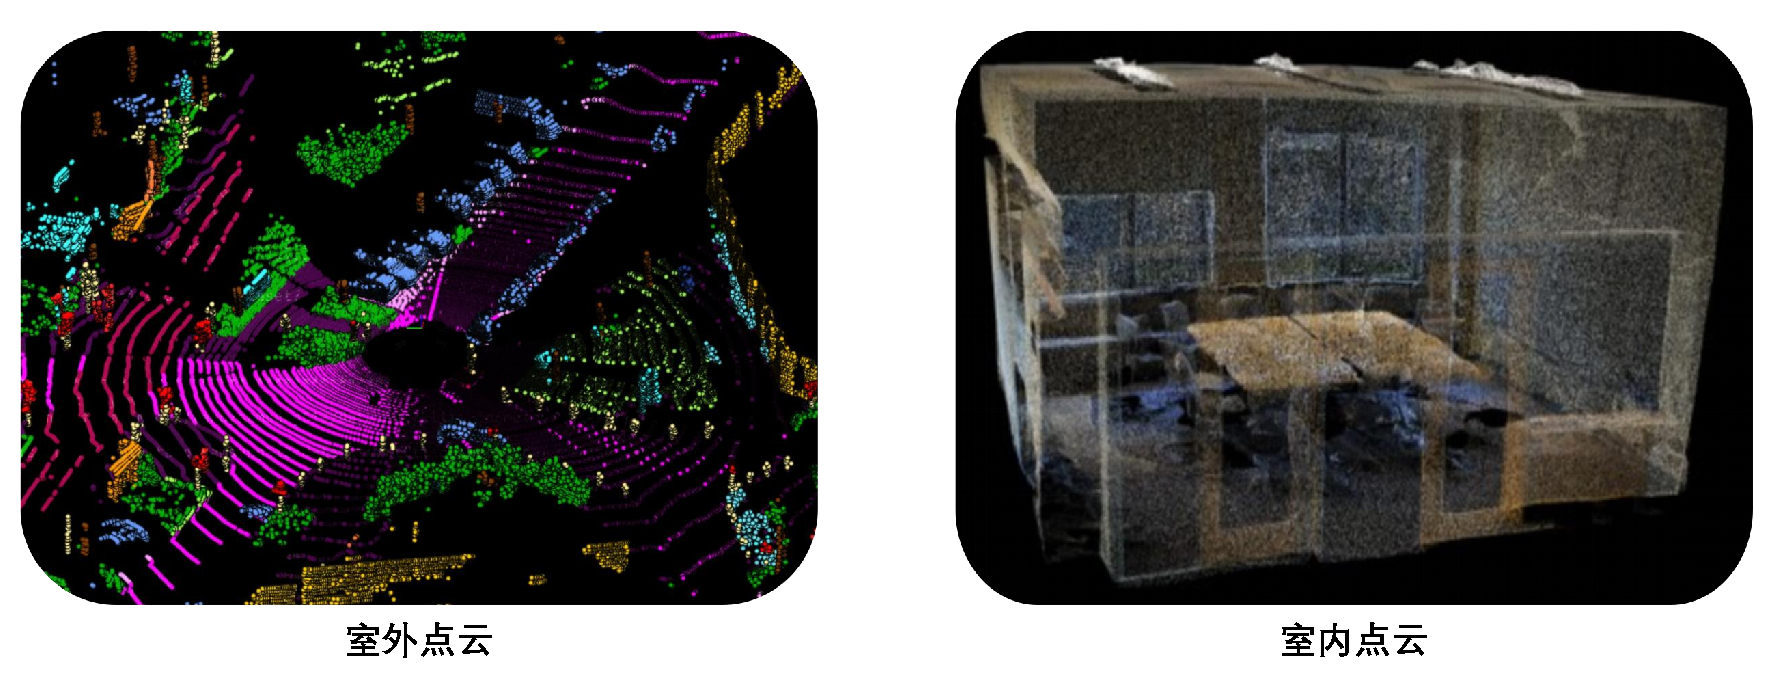
\includegraphics[width = \textwidth, scale=0.5]{ljx/figure/2-1PC.pdf}
    \bicaption[\xiaosi 3D点云]{\wuhao 3D点云}{\wuhao 3D point cloud}
    \label{fig:2-1}
\end{figure}
\vspace{-0.35cm}
\subsection{点云语义分割方法}
\subsubsection{目标与输入数据}
点云语义分割的目标是为三维空间中的每个点赋予特定语义标签。在自动驾驶场景中区分道路、车辆、行人等类别,在室内建模中识别墙面、家具等物体。这一过程本质上是将无序的三维点云转化为带有语义信息的数据。输入的数据通常是由激光雷达(LiDAR)或深度相机采集的原始点云,其基础形式为包含$N$个点的坐标矩阵,形状为$N \times 3$,对应每个点的三维坐标$(x, y, z)$。在一些特殊的场景中,点云可能还包含颜色(RGB值)、反射强度(LiDAR返回信号强度)或时间戳(动态场景中的时序信息)等附加特征,此时数据维度扩展为$N \times D$,其中$D \geq 3$。数据预处理阶段通常会对坐标进行归一化,以消除传感器位姿的影响,并对离群点进行滤波以提高后续处理稳定性。

\subsubsection{特征提取方法}
特征提取是点云语义分割的核心,其目的是从原始点云中挖掘具有判别性的局部与全局特征。根据输入表示方式的不同,主流方法可分为三类:

% \subsubsection{基于点的方法}
1)基于点的方法。
此类方法直接处理原始点云,避免因体素化或投影导致的信息损失。典型代表如PointNet++\upcite{qi2017pointnet++},其核心思想是通过多层感知机(MLP)逐点提取特征,并通过最大池化聚合全局信息。具体而言,对于每个点$\mathbf{p}_i$,模型不仅编码其自身坐标,还通过邻域查询(如k近邻或球查询)收集周围点集$\{\mathbf{p}_j \mid j \in \mathbf{N}(i)\}$,进而利用共享权重的MLP提取局部几何模式,如公式\eqref{eq:2-1}所示:
\begin{equation}
    \label{eq:2-1}
    \mathbf{F}_i = \text{MLP}\left(\mathbf{p}_i - \mathbf{p}_j, \|\mathbf{p}_i - \mathbf{p}_j\|_2\right) \quad \forall j \in \mathbf{N}(i)
\end{equation}
其中$\mathbf{p}_i - \mathbf{p}_j$表示相对位置,$\|\cdot\|_2$为欧氏距离。通过堆叠多个局部特征提取层,模型可逐步扩大感受野,捕获多尺度几何结构。

% \subsubsection{基于体素的方法}
2)基于体素的方法。
基于体素的方法通过将点云转换为规则三维网格实现高效计算。MinkowskiNet\upcite{MinkowskiNet}是该领域的一个代表性方法,其核心是通过稀疏卷积网络,仅对非空体素进行计算,大幅减少内存与计算开销。稀疏卷积的表达式如公式\eqref{eq:2-2}所示:
\begin{equation}
    \label{eq:2-2}
    \mathbf{F}_{\text{out}}(x,y,z) = \sum_{(dx,dy,dz) \in \mathbf{K}} \mathbf{W}(dx,dy,dz) \cdot \mathbf{F}_{\text{in}}(x+dx, y+dy, z+dz)
\end{equation}
其中$\mathbf{K}$为卷积核覆盖的偏移范围,$\mathbf{W}$为卷积核权重。与传统三维卷积不同,稀疏卷积通过哈希表管理非空体素坐标,仅对有效位置执行计算。%例如,MinkowskiNet将输入表示为稀疏张量(包含坐标$C$与特征$F$两部分),计算时仅遍历存在点的体素位置。体素化的分辨率由超参数控制,通常设为$0.05$米至$0.1$米以平衡精度与效率。

% 稀疏卷积的核心优势体现在两方面:
% \begin{itemize}
%     \item \textbf{计算效率}:跳过空体素的计算,尤其适合室外大场景中稀疏点云(如自动驾驶场景中90\%以上体素为空),计算量可降低至密集卷积的1/10。
%     \item \textbf{内存优化}:通过坐标压缩存储(仅记录非空体素位置),避免存储全分辨率三维网格,内存占用与点云密度而非场景体积线性相关。
% \end{itemize}
% 体素化将点云转换为规则的三维网格,便于应用三维卷积操作。例如,VoxelNet将点云划分为$L \times W \times H$的体素单元,每个单元内点云通过小型MLP编码为特征向量,再通过三维卷积进行特征融合:
% \begin{equation}
%     \mathbf{V}_{l+1}(x,y,z) = \sum_{i,j,k} \mathbf{W}(i,j,k) \cdot \mathbf{V}_l(x+i, y+j, z+k) + \mathbf{b},
% \end{equation}
% 其中$\mathbf{b}$为偏置项。体素化的优势在于计算效率高,尤其适合GPU并行计算,但分辨率的限制可能导致细小物体(如电线杆)的细节丢失。为此,稀疏卷积技术被提出以跳过空体素,减少计算冗余。

% \subsubsection{基于投影的方法}
3)基于投影的方法。
此类方法将三维点云投影至二维平面,复用成熟的图像处理网络。其中RangeNet++\upcite{RangeNet++}将LiDAR点云转换为球面距离图像(Range Image),每个像素对应点的深度与方位角。投影后的二维图像通过改进的二维卷积网络提取特征,如公式\eqref{eq:2-3}所示:
\begin{equation}
    \label{eq:2-3}
    \mathbf{F}_{l+1}(u,v) = \text{ReLU}\left(\sum_{m,n} \mathbf{K}(m,n) \cdot \mathbf{F}_l(u+m, v+n)\right)
\end{equation}
其中ReLU为激活函数。投影方法的计算效率较高,但可能因遮挡或投影畸变导致部分三维信息丢失。%为此,部分研究引入多视图融合策略,结合鸟瞰图与前视图提升鲁棒性。

\subsubsection{分类与损失函数}
在特征提取后,模型通过全连接层将$N \times F$维特征映射至$N \times C$维类别得分矩阵,其中$C$为类别总数。Softmax函数将得分转换为概率分布,为每个点分配类别标签,如公式\eqref{eq:2-4}所示:
\begin{equation}
    \label{eq:2-4}
    P(y_i=c) = \frac{e^{\mathbf{z}_{i,c}}}{\sum_{c'=1}^C e^{\mathbf{z}_{i,c'}}}
\end{equation}
其中$\mathbf{z}_{i,c}$表示第$i$个点在第$c$类上的得分。损失函数采用交叉熵损失,衡量预测概率与真实标签的差异,其数学表达式如公式\eqref{eq:2-5}所示:
\begin{equation}
    \label{eq:2-5}
    \mathbf{L} = -\frac{1}{N} \sum_{i=1}^N \sum_{c=1}^C y_{i,c} \log P(y_i=c)
\end{equation}
式中$y_{i,c}$为one-hot编码的真实标签。%针对类别不平衡问题,可采用加权交叉熵损失,为少数类别分配更高权重:
% \begin{equation}
%     \mathbf{L}_{\text{weighted}} = -\frac{1}{N} \sum_{i=1}^N \sum_{c=1}^C w_c \cdot y_{i,c} \log P(y_i=c),
% \end{equation}
% 其中$w_c$与类别频率成反比。此外,动态采样策略(如在训练时对稀少类别点过采样)也被用于缓解数据偏斜。

% \subsubsection{优化挑战与解决方案}
% 点云语义分割面临稀疏性、遮挡与噪声等挑战。例如,在自动驾驶中,远处物体可能仅包含少量点,导致漏检。为此,RandLA-Net提出随机降采样与局部特征聚合策略,在减少计算量的同时保留关键点信息。另一方向是设计轻量化网络(如Cylinder3D),通过柱状分区减少三维卷积计算量,实现实时推理。未来研究可能结合自监督学习,利用未标注数据提升模型泛化能力,或探索多模态融合(如点云与图像融合)以增强语义理解。
% \section{点云语义分割方法}

% \subsubsection{目标与输入数据}
% 点云语义分割的目标是为三维空间中的每个点分配特定语义标签,例如将点标记为树木、建筑物或车辆等类别。输入数据通常是一个包含$N$个点的坐标矩阵,形状为$N \times 3$,分别对应每个点的$x, y, z$坐标。若点云包含颜色或反射强度等附加信息,数据维度扩展为$N \times D$,其中$D$表示特征总数。

% \subsubsection{特征提取方法}
% 特征提取的实现方式根据输入表示分为三类:

% % \subsubsubsection{基于点的方法}
% 1)基于点的方法 
% 直接处理原始点云,利用多层感知机(MLP)对每个点及其邻域进行编码。公式为:
% \begin{equation}
%     \mathbf{F}_i = \text{MLP}\left(\mathbf{p}_i, \{\mathbf{p}_j \mid j \in \mathbf{N}(i)\}\right),
% \end{equation}
% 其中$\mathbf{p}_i$为第$i$个点的坐标,$\mathbf{N}(i)$为其邻域点集合。

% % \subsubsubsection{基于体素的方法}
% 2)基于体素的方法
% 将点云划分为规则三维网格(体素),采用三维卷积提取特征。设体素分辨率为$L \times W \times H$,卷积核尺寸为$k^3$,则特征更新公式为:
% \begin{equation}
%     \mathbf{V}_{l+1}(x,y,z) = \sum_{i,j,k} \mathbf{W}(i,j,k) \cdot \mathbf{V}_l(x+i, y+j, z+k),
% \end{equation}
% 其中$\mathbf{W}$为卷积核权重,$\mathbf{V}_l$为第$l$层体素特征。

% % \subsubsubsection{基于投影的方法}
% 3)基于投影的方法
% 将点云映射到二维平面(如球面投影),使用二维卷积处理。投影后的特征提取公式为:
% \begin{equation}
%     \mathbf{F}_{l+1}(u,v) = \sum_{m,n} \mathbf{K}(m,n) \cdot \mathbf{F}_l(u+m, v+n),
% \end{equation}
% 其中$\mathbf{K}$为二维卷积核,$(u,v)$为投影图像的像素坐标。

% \subsubsection{分类与损失函数}
% 分类阶段将$N \times F$维特征映射到$N \times C$维类别得分,其中$C$为类别数。通过Softmax计算概率分布:
% \begin{equation}
%     P(y_i=c) = \frac{e^{\mathbf{z}_{i,c}}}{\sum_{c'=1}^C e^{\mathbf{z}_{i,c'}}},
% \end{equation}
% 其中$\mathbf{z}_{i,c}$为第$i$个点在第$c$类上的得分。损失函数采用交叉熵:
% \begin{equation}
%     \mathbf{L} = -\frac{1}{N} \sum_{i=1}^N \sum_{c=1}^C y_{i,c} \log P(y_i=c),
% \end{equation}
% 其中$y_{i,c}$为真实标签的one-hot编码。实际应用中需针对类别不平衡问题(如道路点远多于交通灯)优化损失权重或采样策略。当前方法如PointNet++通过局部几何编码提升精度,但对动态遮挡的鲁棒性仍需改进。
\subsection{评价指标}
在点云语义分割任务中,常用的评估指标有两个,一个是总体精度(Overall Accuracy, OA),另一个则是平均交并比(mean Intersection over Union, mIoU)。

总体精度通过计算正确预测点数占总点数的比例,直观反映模型的整体分类能力,其表示式如公式\eqref{eq:2-6}所示:
\begin{equation}
    \label{eq:2-6}
    OA = \frac{TP + TN}{TP + TN + FP + FN}
\end{equation}
其中$TP$表示正确预测的正例,$TN$为正确预测的反例,$FP$为误判的正例,$FN$为误判的正例。尽管OA计算简单,但在点云语义分割中,由于场景中不同类别点数差异显著,如城市道路点占比可能超过50\%,而交通灯可能不足1\%,OA易被多数类别主导,这一缺陷使得OA难以真实评估模型性能。

平均交并比则通过衡量每个类别的预测区域与真实区域的重叠程度,提供更均衡的评估。对于类别$c$,其交并比计算公式如\eqref{eq:2-7}所示:
\begin{equation}
    \label{eq:2-7}
    \text{IoU}_c = \frac{TP_c}{TP_c + FP_c + FN_c},
\end{equation}
其中$TP_c$为类别$c$的正确预测点数,$FP_c$为误判为$c$的点数,$FN_c$为漏判的$c$类点数。mIoU取所有类别IoU的平均值,其表达式如公式\eqref{eq:2-8}所示:
\begin{equation}
    \label{eq:2-8}
    \text{mIoU} = \frac{1}{C} \sum_{c=1}^C \text{IoU}_c
\end{equation}
式中$C$为类别总数,mIoU的核心优势在于其对每个类别的平等关注,即使某一类别的点数极少,其IoU值仍能直接影响整体得分,从而迫使模型兼顾所有类别。
% \subsection{指标选择依据}

当前研究普遍以mIoU为核心评价指标,主要因其能够克服类别不平衡带来的评估偏差。点云数据中,高频率类别与低频率类别的点数差异可能达到数百倍,若依赖OA这类整体指标,模型可能仅通过优化高频类别即可获得高评分,而忽视低频类别的学习,然而对于语义分割任务来说,实现对每一个类别点的精准分割是其目的所在,所以无论低频率类别还是高频率类别都是同等重要。mIoU通过独立计算每个类别的重叠率,确保模型在各类别上的表现均被量化,从而更真实地反映其实际分割能力。此外,mIoU对边界误差的敏感性也优于OA,物体边缘点的误分类会同时增加$FP$和$FN$,导致IoU显著下降,而OA可能因整体正确率高而掩盖此类局部缺陷。%学术界的共识进一步强化了mIoU的地位,主流数据集(如SemanticKITTI、nuScenes)与竞赛均将其作为基准指标,使得不同模型间的横向对比更具一致性。尽管OA仍可作为辅助指标反映整体正确率,但其局限性导致其在最新研究中逐渐边缘化。例如,某模型OA达到95\%但mIoU仅为50\%,仍会被认为未达到实际应用要求。未来,随着细分场景需求的增加,边界IoU或动态加权mIoU等指标可能被引入,以更精准地评估复杂环境下的分割质量。
\section{主动学习基础知识}
% \section{主动学习方法}
% \subsection{主动学习的概念与目的}
主动学习作为传统机器学习中的一个分支,其核心思想是让模型在训练过程中主动选择对提升性能最有价值的数据进行标注,而非被动接受随机标注的数据。该方法的核心目的是在有限标注成本的约束下,通过主动的数据选择策略,最大化模型的性能。%例如,在医学图像分析中,专家标注每张CT图像可能耗时数小时,主动学习可优先选择那些最可能改善肿瘤检测模型性能的疑难样本进行标注,从而减少总标注量。
% \subsection{主动学习的基本流程}
如图\ref{fig:2-2}所示,主动学习的流程可概括为迭代式的“选择-标注-训练”循环。首先,利用初始标注数据训练一个基础的目标模型。随后,模型对未标注数据进行推理预测,生成预测结果。基于这些预测,通过预设的选择策略,从未标注数据中筛选出对当前模型提升最有价值的候选数据。%例如,不确定性采样会选择模型预测概率接近0.5的样本,因其分类边界模糊,标注后能有效修正模型决策边界。
筛选出的候选数据由标注者即该领域相关专家进行标注,新标注数据与原有标注数据合并后,用于更新模型参数。这一过程持续迭代,直至标注预算耗尽或模型性能趋于稳定。流程中的核心模块包括选择策略设计以及模型更新机制,%标注数据管理需平衡新旧数据的分布,避免因过度关注特定样本导致模型偏见。
选择策略的优劣直接决定主动学习效率,常见策略包括不确定性采样、多样性采样和委员会查询。不确定性采样:选择模型预测置信度最低的样本;多样性采样:选择代表数据分布多样性的样本,覆盖不同特征空间区域;委员会查询:训练多个模型,选择各模型预测差异最大的样本。模型更新机制一般考虑如何利用这些已标注的高价值目标点来对模型进行微调以充分发挥数据与模型的潜力。%需考虑增量学习与灾难性遗忘的平衡。例如,在深度学习中,可采用弹性权重固化(EWC)等方法,在更新时保护重要参数不被覆盖。
\vspace{-0.1cm}
\begin{figure}[h]
    \centering
    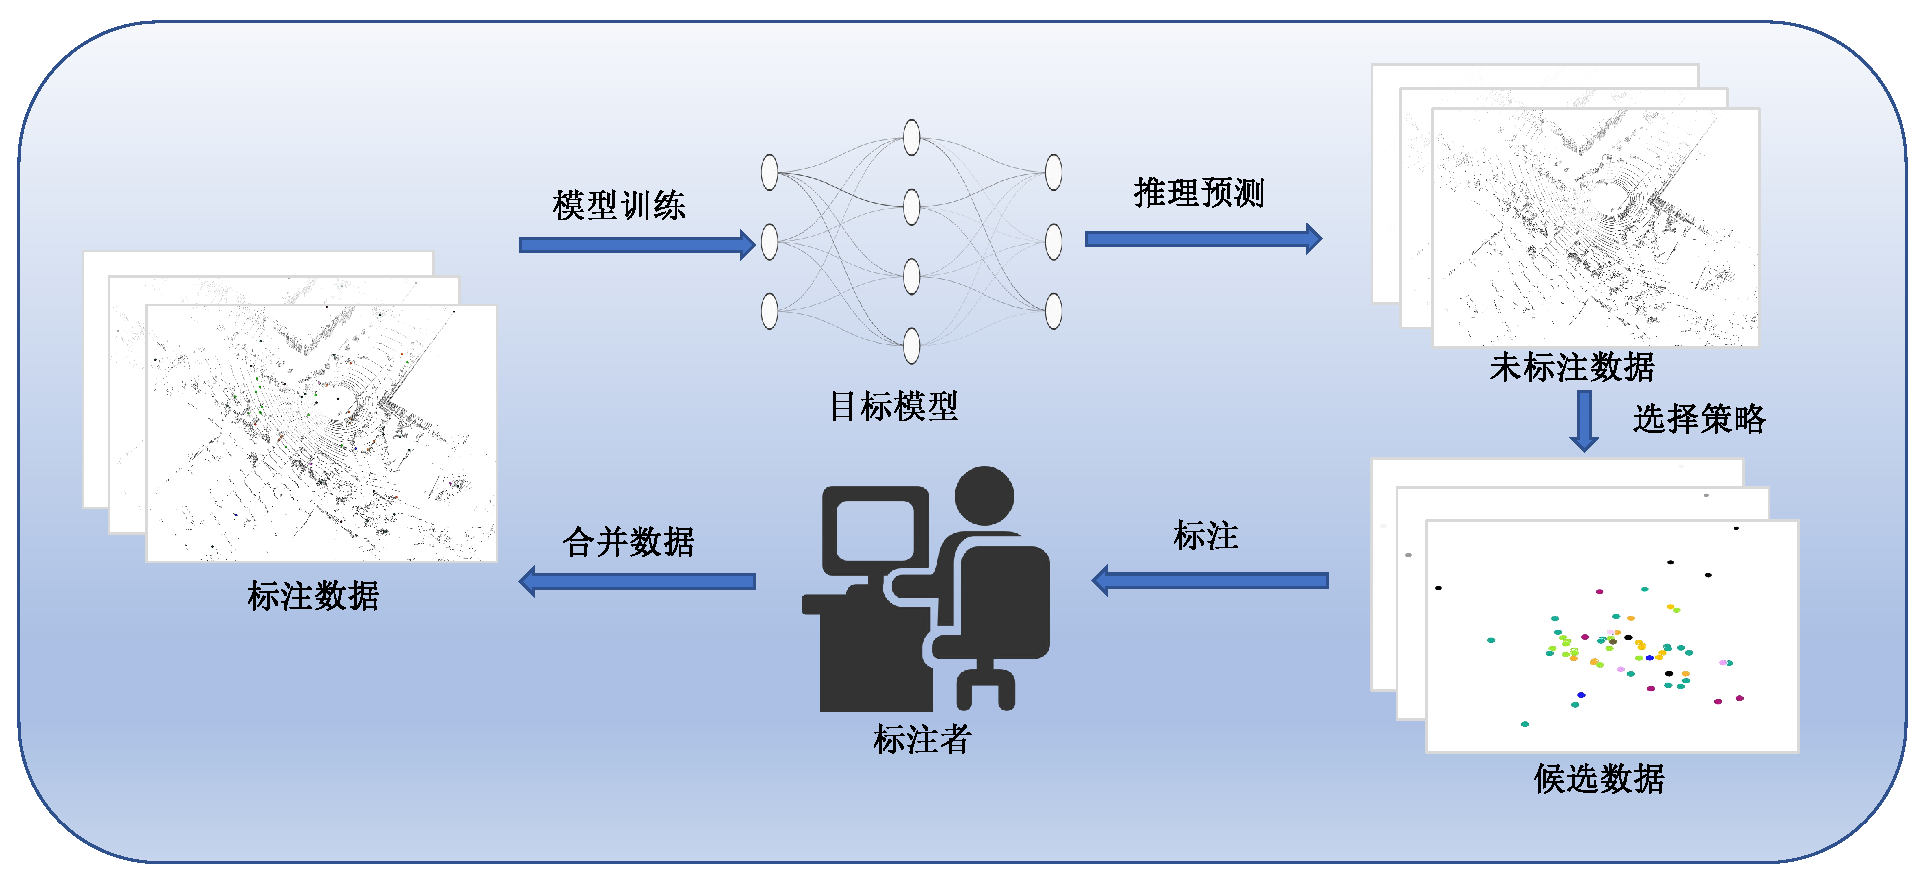
\includegraphics[width = \textwidth, scale=0.5]{ljx/figure/2-2AL.pdf}
    \bicaption[\xiaosi 主动学习]{\wuhao 主动学习}{\wuhao Active learning}
    \label{fig:2-2}
\end{figure}
\vspace{-0.35cm}
% \subsection{应用场景与挑战}
% 主动学习在标注成本高昂或数据分布动态变化的场景中优势显著。例如,自动驾驶中道路标志的标注需适应不同地域、天气条件,主动学习可优先标注罕见场景(如暴雨中的模糊标志)。然而,其挑战在于选择策略的普适性——针对特定任务设计高效策略需领域知识支持。此外,初始模型的质量直接影响后续选择效果,若初始标注数据不足或偏差较大,可能导致选择策略失效。未来研究可能结合自监督预训练,提升初始模型鲁棒性,或设计自适应策略以动态调整选择准则。

\section{域适应基础知识}
% \subsection{域适应的基本概念}
% 域适应(Domain Adaptation)是迁移学习的重要分支,旨在解决源域(Source Domain)与目标域(Target Domain)数据分布不一致导致的模型性能下降问题。假设源域$D_s = \{(x_i^s, y_i^s)\}_{i=1}^{N_s}$包含大量标注数据,而目标域$D_t = \{x_j^t\}_{j=1}^{N_t}$(无监督场景)或少量标注数据$D_t = \{(x_j^t, y_j^t)\}_{j=1}^{N_t}$(半监督场景),域适应的目标是通过对齐两域特征分布,使源域训练的模型$M$能有效泛化至目标域。例如,在自动驾驶中,源域可能为合成点云数据(如CARLA仿真),目标域为真实激光雷达数据,域适应可缩小两者因传感器差异和场景复杂度引起的分布偏移。
% \vspace{-0.1cm}
% \begin{figure}[h]
%     \centering
%     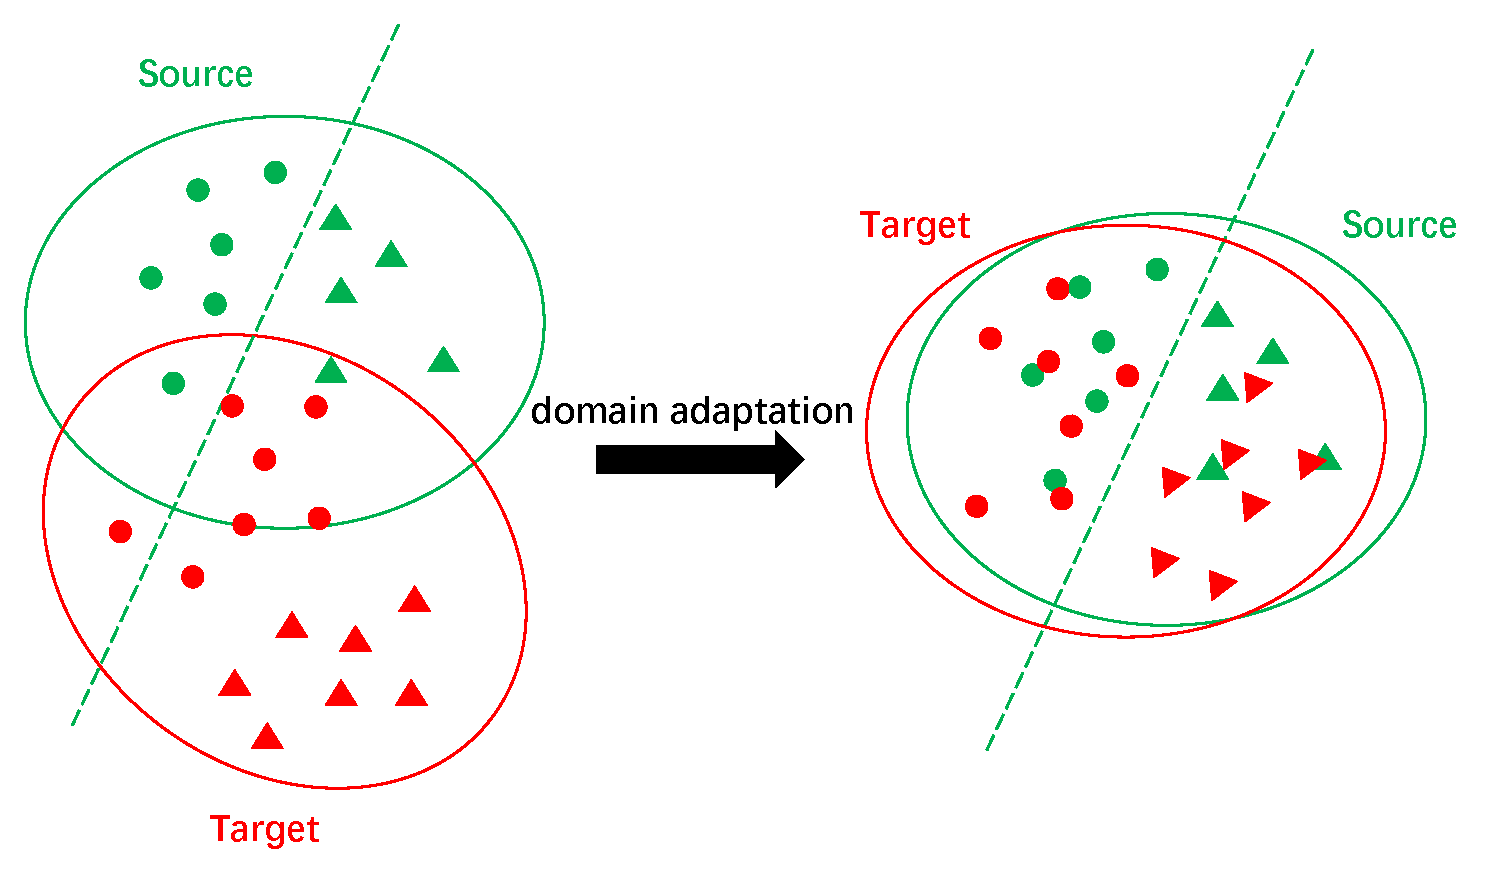
\includegraphics[width = \textwidth, scale=0.5]{ljx/figure/2-3DA.pdf}
%     \bicaption[\xiaosi 域适应]{\wuhao 域适应}{\wuhao Domain adaptation}
%     \label{fig:2-3}
% \end{figure}
% \vspace{-0.35cm}
% \subsection{域适应的核心目标}
% 域适应的核心数学目标是最小化源域与目标域在特征空间中的分布差异,同时保持任务性能(如分类准确率)。定义源域分布为$P_s(x,y)$,目标域分布为$P_t(x,y)$,域适应需实现:
% \begin{equation}
%     \min_{\theta} \underbrace{\mathbb{E}_{(x,y) \sim P_s} \mathbf{L}(f_\theta(x), y)}_{\text{源域任务损失}} + \lambda \cdot \underbrace{d(P_s(x), P_t(x))}_{\text{域差异度量}},
% \end{equation}
% 其中$d(\cdot,\cdot)$为分布距离度量函数,$\lambda$为权衡系数。当目标域无标签时,任务损失仅作用于源域,域对齐成为关键优化方向。
域适应是机器学习中一种重要的技术,主要用于解决模型在相同任务不同数据分布场景下的泛化问题。如图\ref{fig:2-3}所示,当模型在一个数据集即源域上训练得很好,能够正确的将数据分类,但在另一个数据集称为目标域上表现却不佳,无法对目标域中的数据进行正确的分类,而造成这一现象的主要原因是因为不同数据域之间分布不同,存在域间差异,从而导致模型无法对新数据域中的数据进行正确分类,而域适应的目标就是帮助模型适应目标域的数据分布,从而提升其在新数据中的性能。
% 简单来说,当模型在一个数据集即源域上训练得很好,但在另一个数据集称为目标域上表现不佳时,
% 例如,假设我们用一个在晴天采集的自动驾驶点云数据(源域)训练了一个模型,但实际应用中需要处理雨雾天气的点云(目标域),域适应技术可以帮助模型更好地理解雨雾中的障碍物,即使它从未在雨雾数据中直接训练过。
域适应的核心思想是找到源域和目标域之间的共同特征,并通过调整模型或数据,缩小两者之间的分布差异。造成这些差异的原因有很多,比如点云的密度、物体形状的细微变化,或者传感器采集数据的方式不同。
% 举个例子,源域可能是由高精度激光雷达生成的密集点云,而目标域可能来自低成本雷达,点云更稀疏且噪声更多。
域适应的目标就是让模型学会忽略这些差异,而专注于识别共同的特征信息。
% \vspace{-0.1cm}
\begin{figure}[h]
    \centering
    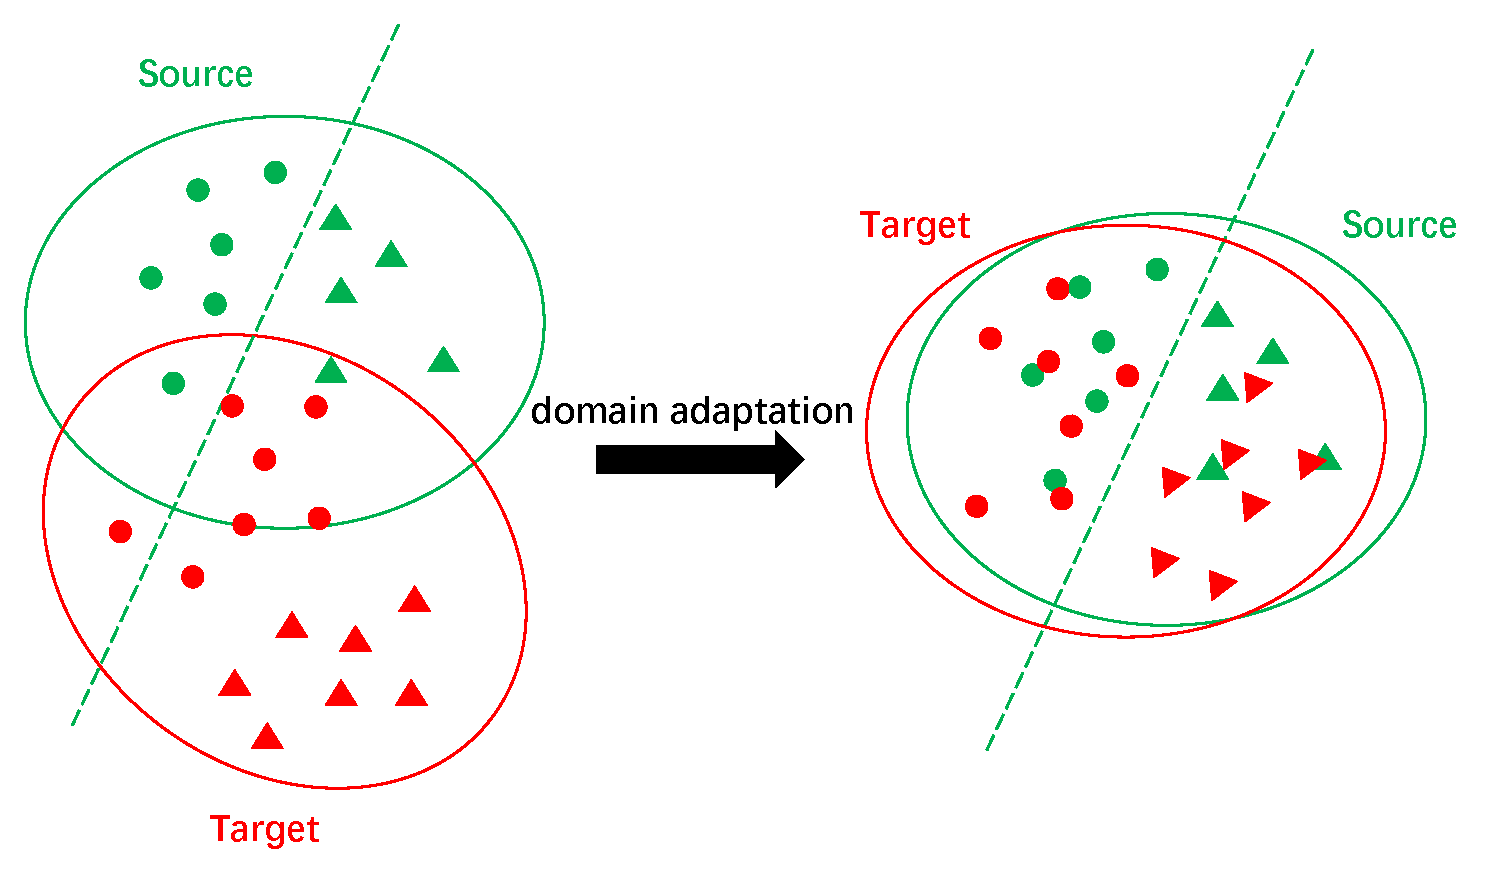
\includegraphics[width = \textwidth, scale=0.5]{ljx/figure/2-3DA.pdf}
    \bicaption[\xiaosi 域适应]{\wuhao 域适应}{\wuhao Domain adaptation}
    \label{fig:2-3}
    \vspace{-0.35cm} 
\end{figure}
% \vspace{-0.35cm} 
\subsection{域对齐的典型方法}
\subsubsection{基于差异度量的域对齐}
% 此类方法显式定义域间分布差异,并通过优化目标函数缩小差异。常用度量包括最大均值差异(Maximum Mean Discrepancy, MMD)和对比域差异(Contrastive Domain Discrepancy, CDD)。对于常用的MMD,其计算两域在再生核希尔伯特空间(RKHS)中的均值差异,表达式如公式\eqref{eq:2-9}所示:
最大均值差异(Maximum Mean Discrepancy, MMD)是一种衡量两个分布之间差异的常用方法,尤其在域适应与生成对抗网络等任务中应用广泛。它的核心思想是先将数据映射到一个称为可再生核希尔伯特空间(RKHS)的高维特征空间中,再比较两个分布在该特征空间中平均嵌入(mean embedding)之间的距离。如果两个分布越相似,它们在该空间中的平均嵌入就越接近;反之则越远。MMD表达式如公式\eqref{eq:2-9}所示:
\begin{equation}
    \label{eq:2-9}
    \text{MMD}^2 = \left\| \frac{1}{N_s} \sum_{i=1}^{N_s} \phi(x_i^s) - \frac{1}{N_t} \sum_{j=1}^{N_t} \phi(x_j^t) \right\|_{\mathbf{H}}^2,
\end{equation}
其中$\phi(\cdot)$是将数据映射到高维空间的核函数,$N_s$,$N_t$分别是源域和目标域的样本数。通过最小化MMD,模型特征提取器$g_\theta$被约束以生成域不变特征。%代发附件发大发积分卡卷发梳福建省大姐夫开始减肥会计师啊咖啡机上岛咖啡结算单甲方按时分无法撒旦法发达防守打法阿斯顿发生代发收到防守打法阿斯蒂芬三大法师代发收到防守打法水电费阿斯蒂芬阿斯顿发生地方发斯蒂芬撒范德萨防守打法阿斯蒂芬撒范德萨发放
\subsubsection{对抗式域适应}
受生成对抗网络(GAN)启发,对抗训练通过域判别器$D$引导特征生成器$g_\theta$混淆域特征,其目标函数为极小极大博弈,如公式\eqref{eq:2-10}所示:
\begin{equation}
    \label{eq:2-10}
    \min_{g_\theta} \max_{D} \mathbb{E}_{x^s}[\log D(g_\theta(x^s))] + \mathbb{E}_{x^t}[\log (1 - D(g_\theta(x^t)))],
\end{equation}
其中$D$试图区分源域与目标域特征,而$g_\theta$试图生成$D$无法区分的特征。而在经典模型对抗域适应网络DANN\upcite{DANN}中,则是将对抗损失与任务损失结合,如公式\eqref{eq:2-11}所示:
\begin{equation}
    \label{eq:2-11}
    \mathbf{L}_{\text{DANN}} = \mathbf{L}_{\text{task}} - \lambda \cdot \mathbf{L}_{\text{adv}}.
\end{equation}

\subsubsection{自训练与伪标签}
自训练利用模型对目标域的预测生成伪标签,逐步迭代优化。定义伪标签为$\hat{y}_j^t = \arg\max_c f_\theta(x_j^t)$,目标域损失表达是如公式\eqref{eq:2-12}所示:
\begin{equation}
    \label{eq:2-12}
    \mathbf{L}_{\text{self}} = \sum_{j=1}^{N_t} \mathbb{I}(\max f_\theta(x_j^t) > \tau) \cdot \mathbf{L}(f_\theta(x_j^t), \hat{y}_j^t),
\end{equation}
其中$\tau$为置信度阈值,$\mathbb{I}(\cdot)$为指示函数。此方法需谨慎设计阈值以避免噪声累积,常与对抗训练结合使用。

\section{跨域点云语义分割数据集}
% 虽然目前开源点云语义分割数据集很多,但是不同的数据集适用于不同的场景,在点云语义分割域适应任务中,通常会选择一些比较流行且大家公认的特定数据集用于进行域适应任务。本研究涉及到合成到真实以及真实到真实两个跨域场景,因此将对这两个场景下的所有数据集都进行介绍,其中合成到真实数据集一般使用合成数据SynLiDAR适应到SemanticPOSS或者emanticKITTI真实数据集上,而在真实到真实跨域场景一般使用真实数据SemanticKITTI与nuScenes进行相互迁移适应。接下来,本小节将分别对以上数据集进行介绍。
% (室外跨域任务,合成到真实常用数据集,真实到真实常用数据集,,以下小节分别对以上数据集进行介绍)
% 虽然目前已有许多开源的点云语义分割数据集,但它们往往适用于不同的应用场景。在点云语义分割的域适应任务中,通常会选择一些流行且广受认可的特定数据集作为实验标准。本研究同时涉及合成到真实(Synthetic-to-Real)和真实到真实(Real-to-Real)两个跨域场景。其中,在合成到真实的跨域场景下,通常使用合成数据SynLiDAR\upcite{xiao2022transfer}迁移至SemanticPOSS\upcite{pan2020semanticposs}或 SemanticKITTI\upcite{behley2019semantickitti}等真实数据集;而在真实到真实的跨域场景中,则一般使用SemanticKITTI与nuScenes\upcite{caesar2020nuscenes}两个真实数据集进行相互迁移适应。以上所涉及的数据集均为室外数据集,接下来本小节将分别对这些数据集进行详细介绍。
虽然目前已有许多开源的点云语义分割数据集,但它们往往针对不同的应用场景设计,具有各自的特点和局限性。在点云语义分割的域适应任务中,通常会选择一些流行且广受认可的特定数据集作为实验标准,以确保结果具有可比性和公平性。本研究同时涉及合成到真实(Synthetic-to-Real)和真实到真实(Real-to-Real)两个跨域场景。在合成到真实的跨域场景下,通常使用合成数据SynLiDAR\upcite{xiao2022transfer}作为源域数据,将其迁移至SemanticPOSS\upcite{pan2020semanticposs}或SemanticKITTI\upcite{behley2019semantickitti}等真实数据集;而在真实到真实的跨域场景中,则一般选择SemanticKITTI与nuScenes\upcite{caesar2020nuscenes}这两个主流的真实数据集进行互相迁移适应。这些数据集均主要反映室外场景的特点,如数据密度、采集角度及环境复杂性等,具有较高的代表性和挑战性。接下来,本小节将对上述数据集的采集背景、数据规模以及在跨域任务中的应用情况进行详细介绍,以便为后续实验提供坚实的数据基础。
\subsection{SynLiDAR}
SynLiDAR是一个大规模的合成LiDAR点云数据集,专为促进从合成数据到真实数据的跨域语义分割研究而创建。该数据集包含超过190亿个逐点标注的点,涵盖32个语义类别,具有丰富的语义信息和高度的几何准确性。与现有的真实LiDAR数据集相比,SynLiDAR的规模更大,质量更高,语义类别更丰富,且标注更加细致和全面。SynLiDAR的点云数据是在多个由专业3D设计师构建的虚拟环境中生成的,这些虚拟环境包含大量与真实世界数据在几何形状和布局上相似的物体模型。如图\ref{fig:2-4}所示,数据集中的每个虚拟场景都经过精心设计,以确保合成数据的高质量和真实性。SynLiDAR的点云数据具有逐点标注,标注类别包括汽车、自行车、摩托车、卡车、其他车辆、行人、骑自行车者、骑摩托车者、道路、停车场、人行道、其他地面、建筑物、围栏、植被、树干、地形、杆、交通标志等,涵盖了丰富的动静态对象,适用于多种语义分割任务。
\vspace{-0.1cm}
\begin{figure}[h]
    \centering
    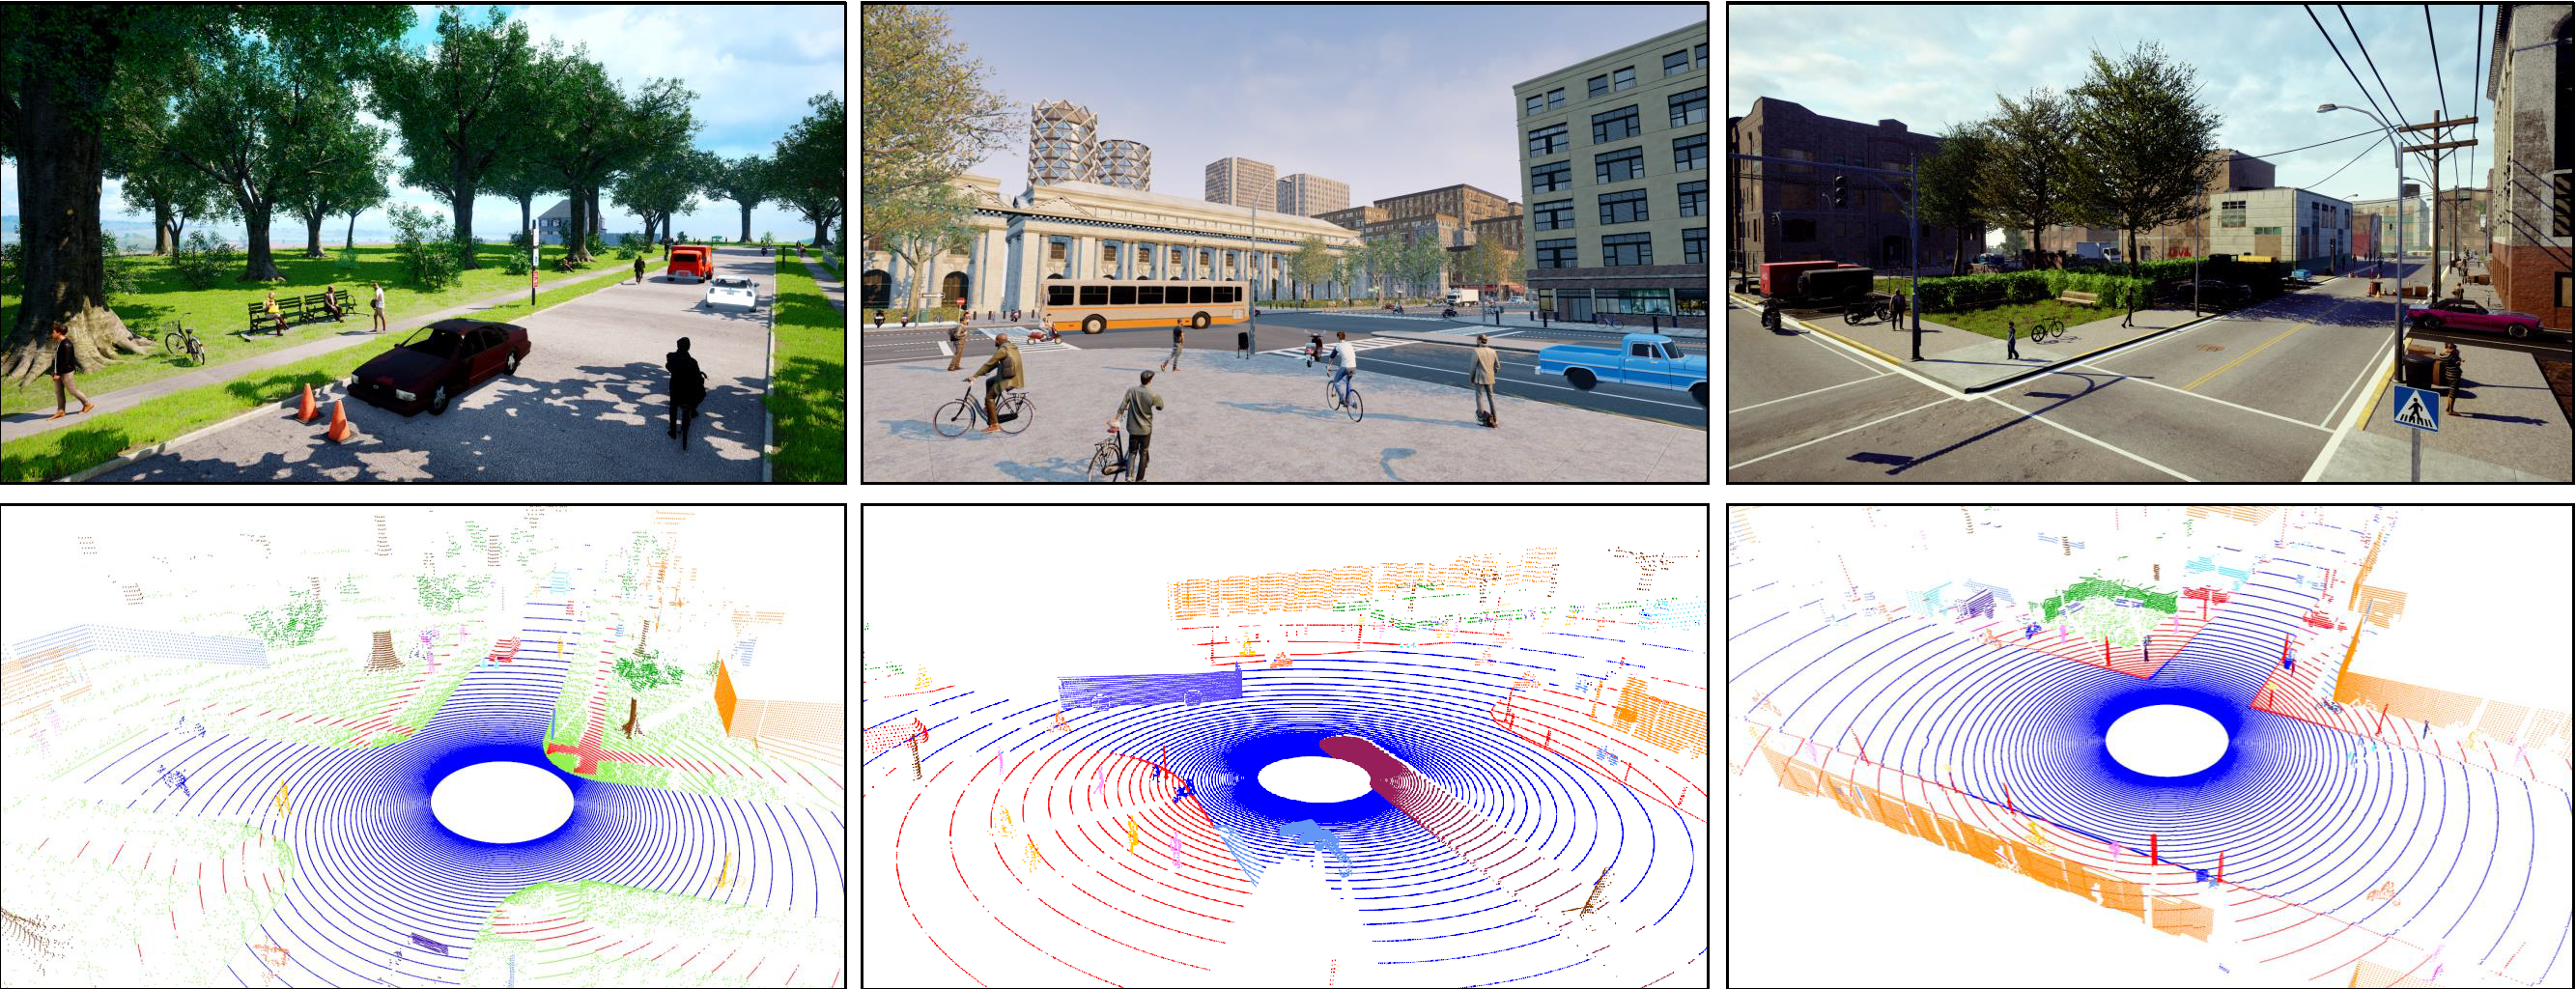
\includegraphics[width = \textwidth, scale=0.5]{ljx/figure/2-5/synlidar.png}
    \bicaption[\xiaosi SynLiDAR数据集\upcite{xiao2022transfer}]{\wuhao SynLiDAR数据集\upcite{xiao2022transfer}}{\wuhao SynLiDAR datasets\upcite{xiao2022transfer}}
    \label{fig:2-4}
\end{figure}
\vspace{-0.35cm} 
\subsection{SemanticKITTI}
SemanticKITTI是一个大规模的室外数据集,是基于真实道路场景构建的激光雷达点云数据集,可用于多种点云分割任务和语义场景补全,与SemanticPOSS相比,该数据集场景更广泛且庞大。其数据通过车载激光雷达采集,包含三维坐标与反射强度信息,但未包含颜色特征。数据集基于 KITTI里程计基准扩展,通过逐点标注实现了360度全景点云的精细化语义标注,涵盖动态与静态对象19个类目标,同时包含地面与可行驶区域等特殊语义类别。
% 涵盖19类目标,包括行人、骑行者、轿车、卡车、道路、人行道、停车场、建筑物、植被、树干、栅栏、杆状物、交通标志等动态与静态对象,同时包含地面与可行驶区域等特殊语义类别。
如图\ref{fig:2-6}所示,数据集共由22个点云序列组成,每个序列都包含一段录制点云。其中,序列00$\sim$10和08总共提供了23201个有标注信息的点云,分别用于训练和验证;11$\sim$21 提供了20351个没有标注信息的点云,用于测试。
点云语义分割域适应中,将SynLiDAR数据集上训练的模型迁移到SemanticKITTIT数据集上,并将类别映射为19个共有的语义类别,包括汽车、自行车、摩托车、卡车、其他车辆、行人、骑自行车者、骑摩托车者、道路、停车场、人行道、其他地面、建筑物、栅栏、植被、树干、地形、杆状物、交通标志。
\vspace{-0.1cm}
\begin{figure}[H]
    \centering
    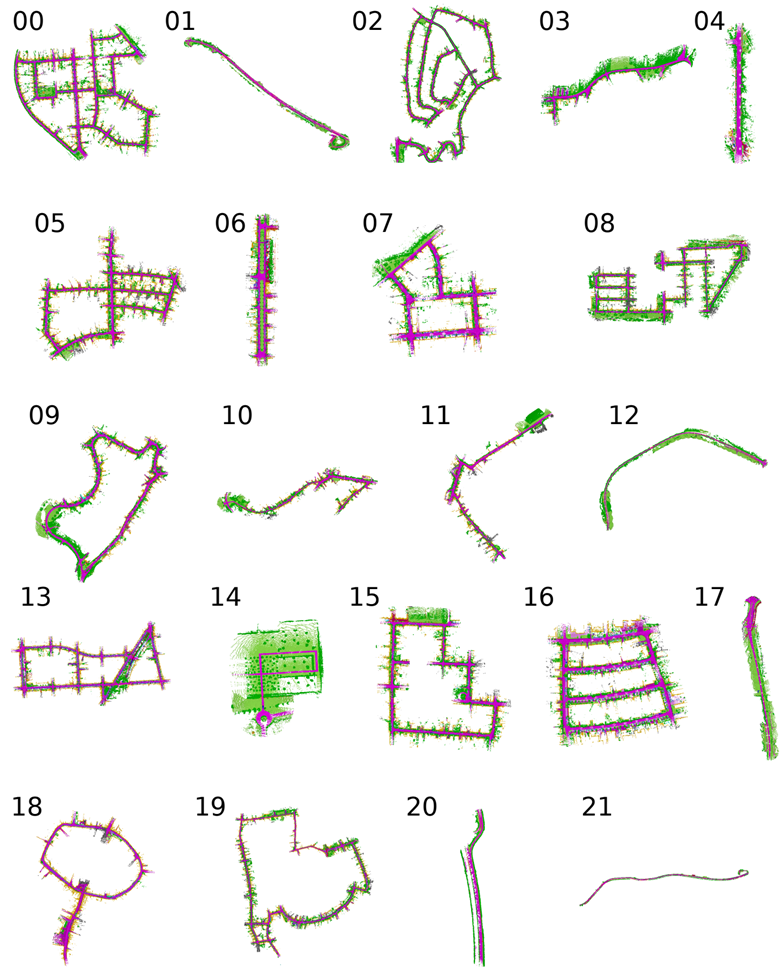
\includegraphics[width = \textwidth, scale=0.5]{ljx/figure/2-5/kitti.png}
    \bicaption[\xiaosi SemanticKITTI数据集\upcite{behley2019semantickitti}]{\wuhao SemanticKITTI数据集\upcite{behley2019semantickitti}}{\wuhao SemanticKITTI datasets\upcite{behley2019semantickitti}}
    \label{fig:2-6}
\end{figure}
\vspace{-0.35cm} 
\subsection{SemanticPOSS}
SemanticPOSS是一个真实世界的小规模数据集,使用Pandora 40线激光雷达传感器在北京大学采集,包含2988个扫描样本。每个扫描样本包含约80,000到100,000个点,捕捉了典型的都市户外场景。该数据集包含13个语义类别,为研究者提供了丰富的数据资源。在数据集划分方面,遵循先验研究的方法,将包含500个点云样本的03序列分配用于验证,而剩余的2488个点云样本则用于训练。在点云语义分割域适应中,将SynLiDAR数据集上训练的模型迁移到SemanticPOSS数据集上,并将类别映射为13个共有的语义类别,包括汽车、自行车、人、骑行者、地面、建筑物、栅栏、植物、树干、杆、交通标志、垃圾桶、路锥/石块。其数据集展示图如图\ref{fig:2-5}所示。
% \vspace{-0.1cm}
\begin{figure}[h]
    \centering
    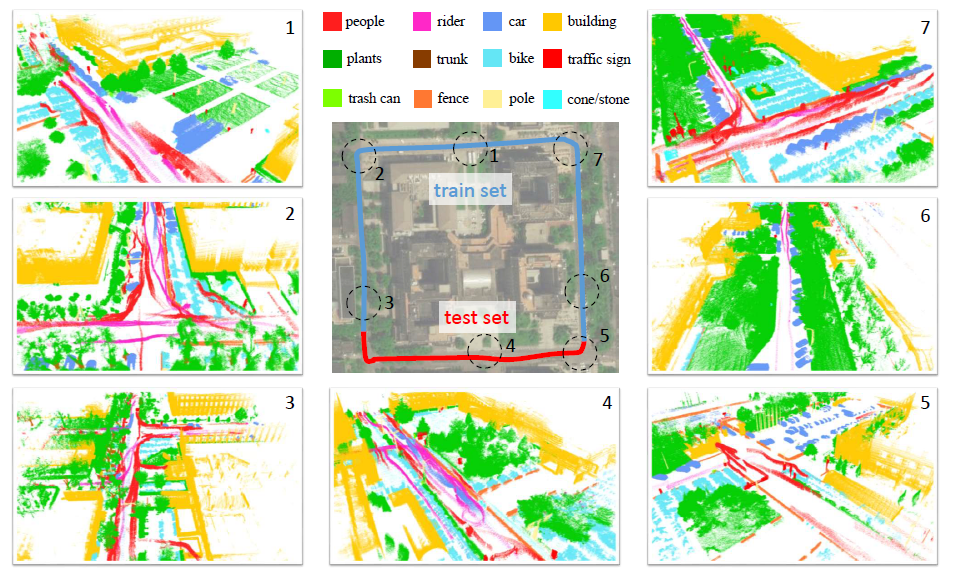
\includegraphics[width = \textwidth, scale=0.5]{ljx/figure/2-5/poss.png}
    \bicaption[\xiaosi SemanticPOSS数据集\upcite{pan2020semanticposs}]{\wuhao SemanticPOSS数据集\upcite{pan2020semanticposs}}{\wuhao SemanticPOSS datasets\upcite{pan2020semanticposs}}
    \label{fig:2-5}
    \vspace{-0.5cm} 
\end{figure}
\subsection{nuScenes}
nuScenes是多模态自动驾驶数据集的代表性资源,整合了激光雷达、摄像头、毫米波雷达及定位系统的同步采集数据,覆盖波士顿与新加坡的1,000个复杂驾驶场景。其激光雷达语义分割子集(nuscenes-lidarseg)包含约14亿个点云,总计40,000帧数据,划分为850个训练验证场景与150个测试场景。语义标注涵盖16类关键目标,包括自行车、公交车、轿车、工程车、摩托车、行人、卡车、拖车等交通参与者,可行驶区域、其他人造地面、人行道、自然地面等道路要素,以及障碍物、锥形路标、植被和人造物体等环境元素。类别设计注重实际驾驶场景的多样性,尤其强调对临时障碍物的精细化标注,例如锥形路标与非铺装路面,为复杂环境下的多目标感知与路径规划提供高精度数据支持。其数据集展示图如图\ref{fig:2-7}所示。
在点云语义分割域适应中,SemanticKITTIT与nuScenes数据进行模型的相互迁移,最终将类别映射为7个共有的语义类别,包括车辆、行人、道路、人行道、地形、人造物体、植被。
\vspace{-0.1cm}
\begin{figure}[h]
    \centering
    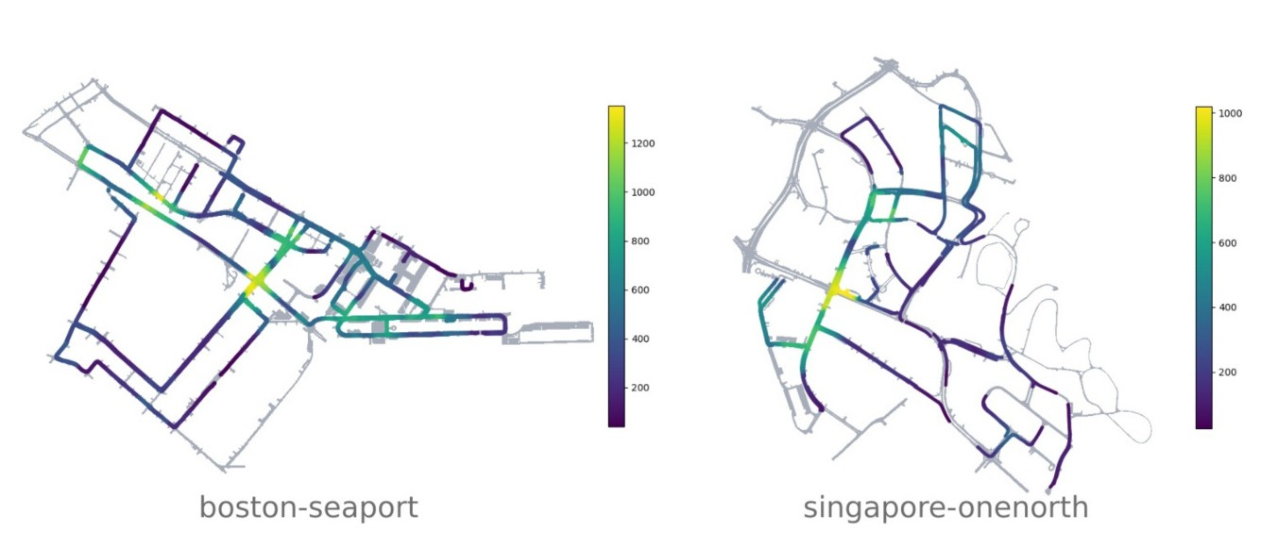
\includegraphics[width = \textwidth, scale=0.5]{ljx/figure/2-5/nuScenes.pdf}
    \bicaption[\xiaosi nuScenes数据集\upcite{caesar2020nuscenes}]{\wuhao nuScenes数据集\upcite{caesar2020nuscenes}}{\wuhao nuScenes datasets\upcite{caesar2020nuscenes}}
    \label{fig:2-7}
\end{figure}
\vspace{-0.35cm} 
\section{本章小结}
本章主要对点云语义分割主动域适应相关领域的基础知识做了全面介绍,包含对点云语义分割,主动学习,域适应在内的多个不同领域分别做了介绍。 对于点云语义分割的相关基础知识,首先详细介绍了点云的获取方式、点云的特征以及室内外点云的差异。根据特征提取方式的不同,进一步对点云语义分割任务的基本模型和基本实现方式做了基础介绍,最后还介绍了语义分割任务中常用的评价指标mIoU。对于主动学习相关基础知识,主要对主动学习方法的基本概念和基本流程做了详细阐述;针对域适应基础知识,首先介绍了域适应的概念、目的以及任务,接着又对常见的域对齐方法进行了梳理和解释。最后还对点云语义分割域适应任务中常用的室外跨域数据集分别进行了介绍。本章介绍的各方面基础知识对后续章节中算法设计的阅读理解起到重要铺垫作用。
% 可在此增加文字以增加页数

% 第3章


\chapter{基于点云语义分割域适应的主动学习方法}
\thispagestyle{others}
\pagestyle{others}
\xiaosi

\section{本章引言}
本章主要介绍一种新的用于点云语义分割域适应的主动学习方法,该方法提出了一种基于源域原型指导的主动查询策略,并结合Mixing方法构建出强壮的中间域数据,极大的提高了点云语义分割域适应模型的性能。接下来,本章节将首先介绍方法的研究动机和贡献,接着对每个子方法模块的原理及实现细节进行详细的介绍,最后本文将通过在主流公开数据集上取得的实验结果以及对消融实验的分析展示方法的有效性。

\section{研究动机及贡献}
% 近年来,基于深度学习的点云语义分割方法在单一域场景下取得了显著进展,但
% 其性能高度依赖于大量标注数据。然而在实际应用中,训练的数据集与从真实环境中获取的数据集由于传感器配置、场景的不同,会产生域间隙
% 然而,在跨域场景中,目标域标注数据往往是
% 稀缺或者没有的,因此如果进行逐点人工标记则会耗费大量的人力物力,而由于域差异的存在不能直接将,所以现有方法往往面临显著的
% 域间分布差异,导致模型在目标域上的泛化能力急剧下降。而一些传统单域主动
% 学习方法\upcite{Entropy,Margin}通过选择信息量最大的样本进行标注,能够有效缓解标注成本问题。
% 然而,这些方法的样本选择策略都假定在单模态源域分布上,忽略了潜在的多模态
% 分布,而这会导致模型选择次优的目标样本并影响性能\upcite{MADA}。
% 第一,现有图像领域的主动域适应方法(如基于不确定性的边界采样[12]或基
% 于对抗学习的特征对齐[24])难以直接迁移至点云场景。点云数据具有不规则性、
% 稀疏性和几何结构敏感性,其三维空间中的局部语义关联与二维图像存在本质差
% 异。例如,图像中基于像素块或超像素的主动查询策略无法有效捕捉点云局部邻
% 域的非欧氏特征分布,导致跨域场景下的信息量评估不准确。

% 先说一些传统主动学习,然后说这些方法不适用于多模态的域适应中引用,然后说一些人开始研究新的主动域适应方法,然后举一些图像上的例子,并说明这些方法都无法直接用于点云,然后点云研究非常的少,因此探索这块领域说出问题。基于上述分析,本章的方法怎么做的相比之前的方法有何不同,提出创新性,考虑到数据的增强方式,结合mixing策略,它的优势,并且突出于mixing与AL的结合是第一次的。

% -什么方法解决了什么问题
% 介绍一下之前的方法,主动学习介绍一下,存在问题,由于域偏差的存在,不能
% 直接运用于域适应,然后主动域适应介绍一下,并没有专门的点云
% 主动域适应的策略,(介绍一些最新图像的,然后说明这些方法不适用于点云),
% 然而点云的数据结构不同于图像,由于数据模态的不同,其数据量的不同,往往
% 点云的数据量会更大,图像上的方法无法直接应用到3D点云,而在3D点云语义分
% 割中对这些方法缺乏相应的研究
% -因此本文提出了一种主动域适应策略
% -传统的主动学习方法

% 近年来,在人工智能与计算机视觉领域蓬勃发展的当下,语义分割技术作为关键的视觉任务,其重要性不言而喻。尤其是基于深度学习的语义分割方法,在图像和点云数据处理方面都取得了令人瞩目的成果。然而,这些高性能的方法往往依赖于大规模标注数据的支撑。对于三维点云而言,获取逐点标注数据是一项极为繁琐、昂贵且耗时的工作,这严重制约了相关算法的实际应用和推广。
% 为了降低标注成本并提高模型性能,主动学习方法被引入到点云语义分割任务中。现有的主动学习方法在点云语义分割领域取得了一定的进展,【】【】【】,然而,这些方法的样本选择策略都假定在单模态源域分布上,忽略了潜在的多模态分布,而这会导致模型选择次优的目标样本并影响性能\upcite{MADA}。
% 为了解决上述问题,一些学者开始致力于主动域适应的方法的研究,并在图像语义分割领域取得了一定的成果,【xxx提出】【xxx提出】然而些方法大多不能直接应用于点云语义分割。一方面,点云数据具有独特的几何结构和稀疏性,与图像数据的网格结构有本质区别;另一方面,点云的数据量庞大且无序,直接迁移图像领域的主动域适应方法无法有效捕捉点云的关键特征。
% 针对上述问题,本章提出了一种用于点云语义分割域适应的主动学习方法。该方法通过构建源域原型来指导目标点的选择,与传统主动学习方法相比,能够更有效地选择出与源域偏离程度更高的目标点,这些点往往是减小域差异的关键。此外,为了进一步提升模型的泛化能力,将主动学习与混合方法相结合,构建出包含源域和目标域选择点组成的强健中间域数据,进一步缩减域间隙。

% 本章节研究内容的主要贡献如下

% 1)提出了首个面向点云语义分割域适应的主动学习方法,超过了结合传统主动学习方法的点云语义分割域适应结果,并在极少量的标注下取得了超过最先进方法的结果。

% 2)提出了一种源域指导的目标点主动选择策略,计算目标域中候选点与源域的偏离程度,从而选择出。

% 3)将主动学习与mixing方法进行结合,构建强健的中间域数据,进一步缩减域间隙

% \section{研究动机及贡献}  
近年来,三维点云语义分割技术在自动驾驶、智能机器人等领域的应用需求日益迫切。尽管基于深度学习的全监督方法在点云语义分割上取得了显著性能,但其实际部署面临两大核心挑战:标注成本瓶颈与域间分布差异。一方面,点云的逐点标注需耗费大量人力物力,标注单帧车载激光雷达点云需约2小时\upcite{behley2019semantickitti}。而真实场景中目标域数据因传感器配置、环境动态变化等因素,与源域存在显著分布偏移,导致模型泛化性能急剧下降\upcite{yuan2024density}。  

为缓解标注压力,现有研究主要沿两条路径展开:主动学习通过选择最具代表性的样本进行标注,以最小标注代价提升模型性能;无监督域适应则尝试在无目标域标注下对齐源域与目标域特征分布。然而,两者在跨域场景中均存在固有局限。传统主动学习方法\upcite{Entropy,Margin,settles2009active}的样本选择策略都假定在单模态源域分布上,忽略了潜在的多模态分布,因此选择的样本无法有效指导域间特征对齐,这会导致标注资源浪费并影响模型性能\upcite{MADA,Divide}。无监督虽无需目标域标注,但其依赖于大量的伪标签,而伪标签噪声会随迭代过程累积,限制性能提升,导致其与全监督基线仍存在很大的差异。

针对上述存在的问题,一些学者开始致力于主动域适应方法研究\upcite{AADA,CLUE,EADA能量工程},其结合主动学习和域适应方法的优势,并在图像语义分割领域取得了一定的成果,然而些方法大多不能直接应用于点云语义分割。一方面,点云数据具有独特的几何结构和稀疏性,与图像数据的网格结构有本质区别;另一方面,点云的数据量庞大且无序,直接迁移图像领域的主动域适应方法无法有效捕捉点云的关键特征。在三维点云中,Annotator\upcite{Annotator}提出了一种以体素为中心的主动学习方法,用以选择显著且具有代表性的体素,并随后对这些体素内的所有点进行标注。它第一次将主动学习运用到三维点云语义分割域适应中,并取得了超越其他传统主动学习方法的效果,然而它只考虑了点云特性依然忽略了域间差异。

% 3. **跨模态方法的不可迁移性**  
%    图像领域的主动域适应方法(如基于类原型对齐的AADA\upcite{su2020active}或对抗性查询\upcite{prabhu2021ada})难以直接迁移至点云任务。点云数据具有**非结构化、稀疏性**及**几何敏感性**等特性:  
%    - 图像超像素划分或区域提案策略无法捕捉点云局部邻域的几何关联(如曲率连续性);  
%    - 基于RGB特征的域差异度量忽略点云独有的反射强度、深度分布等模态信息;  
%    - 现有混合增强方法(如CutMix\upcite{yun2019cutmix})破坏点云空间连续性,导致语义上下文丢失\upcite{xiao2022polarmix}。  

通过上述分析,本章提出基于点云语义分割域适应的主动学习方法,核心思想是通过源域原型指导目标域上点的选择,并将标注后的目标点与源域点进行混合,组成中间域数据,实现标注效率与域对齐能力的协同优化。构建以下两个模块:1)域差异感知的主动查询:通过动态构建源域类别原型以代表源域,计算目标域中候选点与源域的偏离程度,筛选同时具备高不确定性与高域差异的目标点。这些样本能够精准暴露域间分布边界,指导模型聚焦于域偏移敏感区域。2)动态中间域构建:引入Mixing方法,随机从源域中采样一定比例的标注点与已标注的目标点云进行混合增强,生成兼具双域信息的中间域数据,该方法增强模型对域不变特征的提取能力,可以进一步缩减域间隙。
% 2. 动态中间域构建:为避免源域数据淹没稀疏标注的目标域信息,提出一种混合策略——随机采样与标注目标点等量的源域点云进行拼接,生成兼具双域统计特性的中间域数据。该策略通过隐式特征插值增强模型对域不变特征的提取能力,同时抑制源域主导的过拟合风险。  

% 本章贡献可归纳为:  

% 1)提出首个面向点云语义分割的主动域适应框架**,通过联合优化域差异感知标注与跨域混合训练,在目标域标注量仅为1\%时,mIoU超越现有UDA方法12.7\%,接近全监督基准的95\%。  

% 2)设计源域原型引导的主动查询机制**,基于类中心对齐量化目标点域偏离度,相比传统熵采样策略,在跨域任务中标注效率提升30\%(以单位标注量的mIoU增益衡量)。  

% 3)首次将主动学习与mixing方法进行结合,构建强健的中间域数据,进一步缩减域间隙  


本章节研究内容的主要贡献如下:

1)提出了以个面向点云语义分割域适应的主动学习方法,超过传统主动学习方法下的点云语义分割域适应结果,并在极少量的标注下取得了超过最先进方法的结果。

2)提出了一种源域指导的目标点主动选择策略,筛选出兼具高不确定性和高域差异的目标点。

3)首次将主动学习与Mixing方法进行结合并运用到域适应领域,动态构建包含双域信息的中间域数据,进一步缩减域间隙。

% 方法优势与创新性:
% 与单域主动学习相比,本方法显式建模域间差异,避免标注由域偏移引起的伪不确定点;与被动域适应相比,通过主动标注关键目标域样本,构建强监督信号引导特征对齐。实验表明,该方法在复杂跨域场景(如昼夜转换、多城市迁移)中均表现出显著鲁棒性,为低标注成本下的三维场景理解提供了新的技术路径。

\section{基于原型指导的主动学习方法}
\subsection{问题陈述}
在点云语义分割域适应任务中,给定一个标注的源域数据\(\mathcal{S} = \{(\mathbf{X}_i^s, \mathbf{Y}_i^s)\}_{i=1}^{N^S}\),和一个目标域数据$\mathcal{T} = \{(\mathbf{X}_i^t)\}_{i=1}^ {N^T}$,其中\(N^T\)和\(N^S\)分别代表目标域和源域点云帧的数量,$\mathbf{X}_i \in \mathbb{R}^{{n_i} \times 4}$代表含有$(x,y,z,i)$三维坐标点和反射强度的一帧点云集合,并且$n_i$代表在第$i$帧点云中点的数量。 域适应的目标则是在主动学习方法的帮助下,将从标注的源域上训练好的模型$\mathcal{G}$迁移泛化到目标域数据上来,并在目标域上实现准确的点云语义分割。

在主动域适应场景中,给定一个未标注的目标域数据集$\mathcal{T}$,需要从中筛选出能够代表目标域且信息量最大的数据子集进行标注。利用新标注的目标域数据,源域训练的分割模型可逐步迭代调整以适应目标域分布,最终实现目标域上的精确语义分割。具体流程如下:首先,基于预训练模型$\mathcal{G}$对目标域数据的预测结果,设计查询策略以计算每个未标注目标点的代表性度量得分;随后,选择最具代表性的目标点子集\(\mathcal{T}_l\)进行标注,并利用其参与分割模型 $\mathcal{G}$的调优,同时更新未标注目标数据集\(\mathcal{T}=\mathcal{T}-\mathcal{T}_l\)。该过程循环迭代直至达到预设的主动学习预算$B$。 
\subsection{方法概述}
本方法的总体框架如图\ref{fig:framework-3}所示。其算法流程主要由三个模块构成:
\ding{172}源域原型构建:通过分割模型从源点云中提取特征,并基于这些特征构建源域原型,并将作为源域的语义表征代表源域。
\ding{173}源原型引导的数据选择:计算未标记的目标点到原型的特征空间距离,得到原型相似度特征图,并根据最优-次优差异算法生成域差异分数,并将此分数与模型预测的不确定性分数结合,生成最终评分以指导标注候选目标点的选择。
\ding{174}动态混合中间域构建:使用Mixing方法,随机从源域中采样一定比例的标注点与已标注的目标点进行混合增强,生成兼具双域信息的中间域数据,并将此数据用于分割模型的微调。

\vspace{-0.1cm}
\begin{figure}[h]
    \centering
    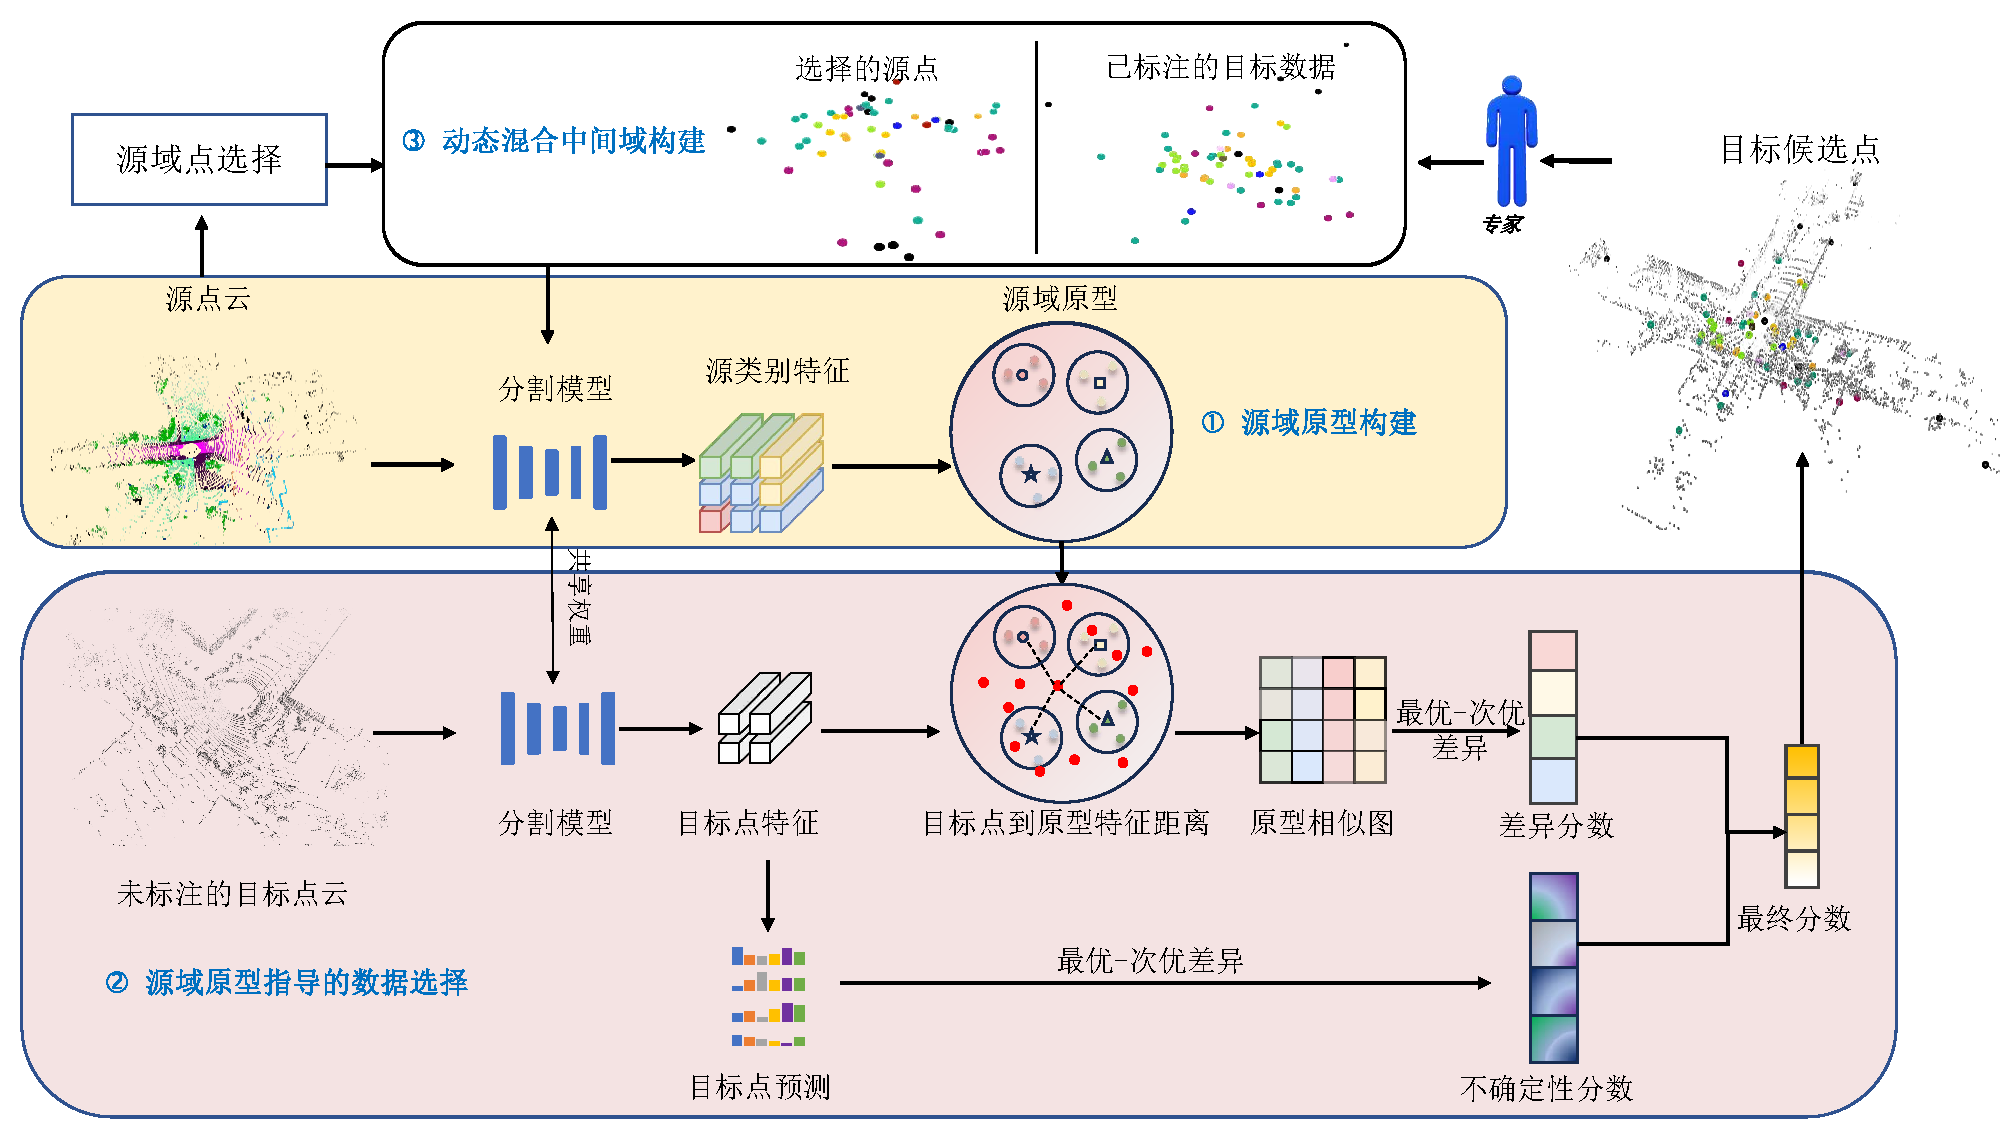
\includegraphics[width = \textwidth]{ljx/figure/3-1.pdf}
    \bicaption[\xiaosi 基于点云语义分割域适应的主动学习方法框架]{\wuhao 基于点云语义分割域适应的主动学习方法框架}{\wuhao Framework of the active learning method for domain adaptation in point cloud semantic segmentation}
    \label{fig:framework-3}
\end{figure}
\vspace{-0.35cm}

\subsection{源域原型构建}
% 当前面向点云语义分割的主动域适应方法主要利用源域预训练模型在目标域的预测结果,通过识别模型难以准确判别的"不确定性"数据来选择标注样本。然而,这类方法存在两个关键缺陷:首先,其选择过程忽略了源域与目标域之间的分布差异,导致所选样本往往集中在特定长尾类别上,使得标注数据缺乏多样性和代表性;其次,源域训练的分割模型对目标域数据的预测存在偏差,导致查询策略的可靠性降低。
% 为此,本章提出通过联合考虑预测置信度与源-目标域分布差异,实现可靠且分布均衡的数据选择。
为表征源域数据分布的结构特征,首先需要基于特征中心构建源域类别原型。具体而言,对于源域中每个类别的点云样本,利用分割模型$\mathcal{G}$,提取其特征向量,并将同类特征向量的均值作为该类的原型表征。如图\ref{fig:3-2}所示,将标注的源域数据集$\mathcal{S}$输入当前网络$\mathcal{G}$,提取特征矩阵$\mathbf{F} \in \mathbb{R}^{{N^S_P} \times d_f}$, 其中\(N^S_P\)表示源域中所有标注类别点的数量,$d_f$为特征维度,基于源数据类别信息,通过公式\eqref{eq:prototype_compute}所示计算类别原型\( \mathbf{p}^c \):
\begin{equation}
    \label{eq:prototype_compute}
    \mathbf{p}^c = \frac{\sum_{i=1}^{N^c} \mathbf{f}_i^c}{N_c}
\end{equation}
其中,\( c \in [1, C] \)表示类别索引,\( C \)为源域类别总数;\( \mathbf{f}_i^c \)为类别\( c \)中第\( i \)个点的特征向量;\( N_c \)为类别\( c \)的样本数量,对应的公式如\eqref{eq:Nc}所示:
\begin{equation}
    \label{eq:Nc}
    % N_c = \sum_{\mathbf{f} \in \mathbf{F}} \mathbb{I}(\mathbf{f} = c),
    N_c = \sum^{N^S_P}_{i=1} \mathbb{I}(y^s_i = c)\mathbf{f}_i
\end{equation}
其中\( y^s_i \)表示第\(i\)个源点特征\( \mathbf{f}_i \)对应的类别标签,$\mathbb{I}(y^s_i = c)$为指示函数,当$y^s_i$属于类别$c$时取值为1,否则为0。

由于点云数据集庞大,因此常规服务器设备无法一次性将所有的数据都加载到内存并进计算,而如果设计全局变量累加多次迭代的结果,可能会造成一定的精度损失和内存消耗,为了节省内存资源和保证结果的准确性,本章采用Welford增量均值算法\upcite{welford1962note}进行渐进式的原型计算,如公式\eqref{eq:incremental_equation}所示:
\begin{equation}
\label{eq:incremental_equation}
    \mathbf{p}_{b+1}^c = \mathbf{p}_b^c + \frac{\mathbf{p}_{b+1}^c - \mathbf{p}_b^c}{x_{b+1}}
\end{equation}
式中,\(\mathbf{p}_{b+1}^c\)代表在第\(b+1\)训练批次时类别\(c\)的原型结果,\(\mathbf{p}_{b}^c\)代表上一批次时类别\(c\)的原型结果,\( x_{b+1} \)则代表在第\( b+1 \)训练批次时类别\( c \)的总数量。通过该算法最终得到源域原型矩阵\( \mathbf{P} \in \mathbb{R}^{C \times {d_f}} = \{\mathbf{p}^i\}^C_{i=1} \),其中每个原型向量\(\mathbf{p}^i\)对应特征空间中源域某类别的质心,蕴含该类别的语义特征。这些原型将在每一轮的主动学习阶段动态更新,为跨域数据选择提供指导。

\vspace{-0.1cm}
\begin{figure}[h]
    \centering
    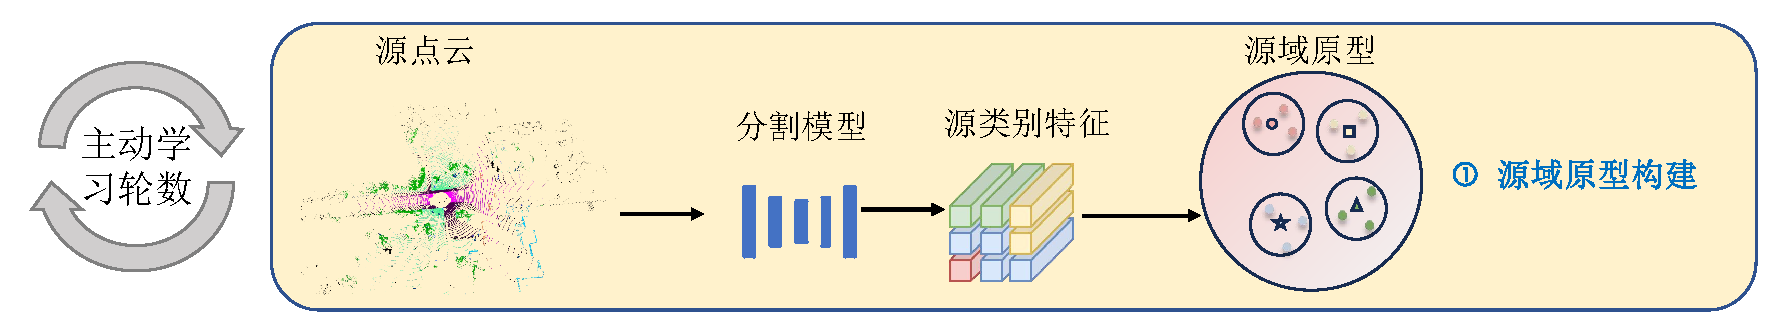
\includegraphics[width = \textwidth]{ljx/figure/3-2.pdf}
    \bicaption[\xiaosi 源域原型构建]{\wuhao 源域原型构建}{\wuhao Source prototype construction}
    \label{fig:3-2}
\end{figure}
\vspace{-0.35cm}


\subsection{源域原型指导的数据选择}
源域原型构建完成后,可将其作为基准指导目标域数据的筛选。如图\ref{fig:3-3}所示,将未标注的目标域点云输入预训练分割网络,提取其特征矩阵\( \mathbf{F}^T \in \mathbb{R}^{N^T \times d_f} \),其中\(N^T\)为目标域点数。随后逐点计算其与源域各类别原型的欧氏距离,其表达式公式为\eqref{eq:distance}:
\begin{equation}
    \label{eq:distance}
    \mathbf{d}_i^c = \| \mathbf{f}_i^t - \mathbf{p}^c \|
\end{equation}
式中\( \mathbf{f}_i^t \in \mathbf{F}^T \)表示目标域第\( i \)个未标注点的特征向量,\(\mathbf{p}^c\)为源域类别\(c\)的原型向量。\( d_i^c \)代表点到源域类别\(c\)的欧式距离,该距离度量反映了目标点特征与源域类别质心的空间匹配度:距离越小,表明目标点特征在源域特征空间中越接近类别\( c \)的聚类中心。
\vspace{-0.1cm}
\begin{figure}[h]
    \centering
    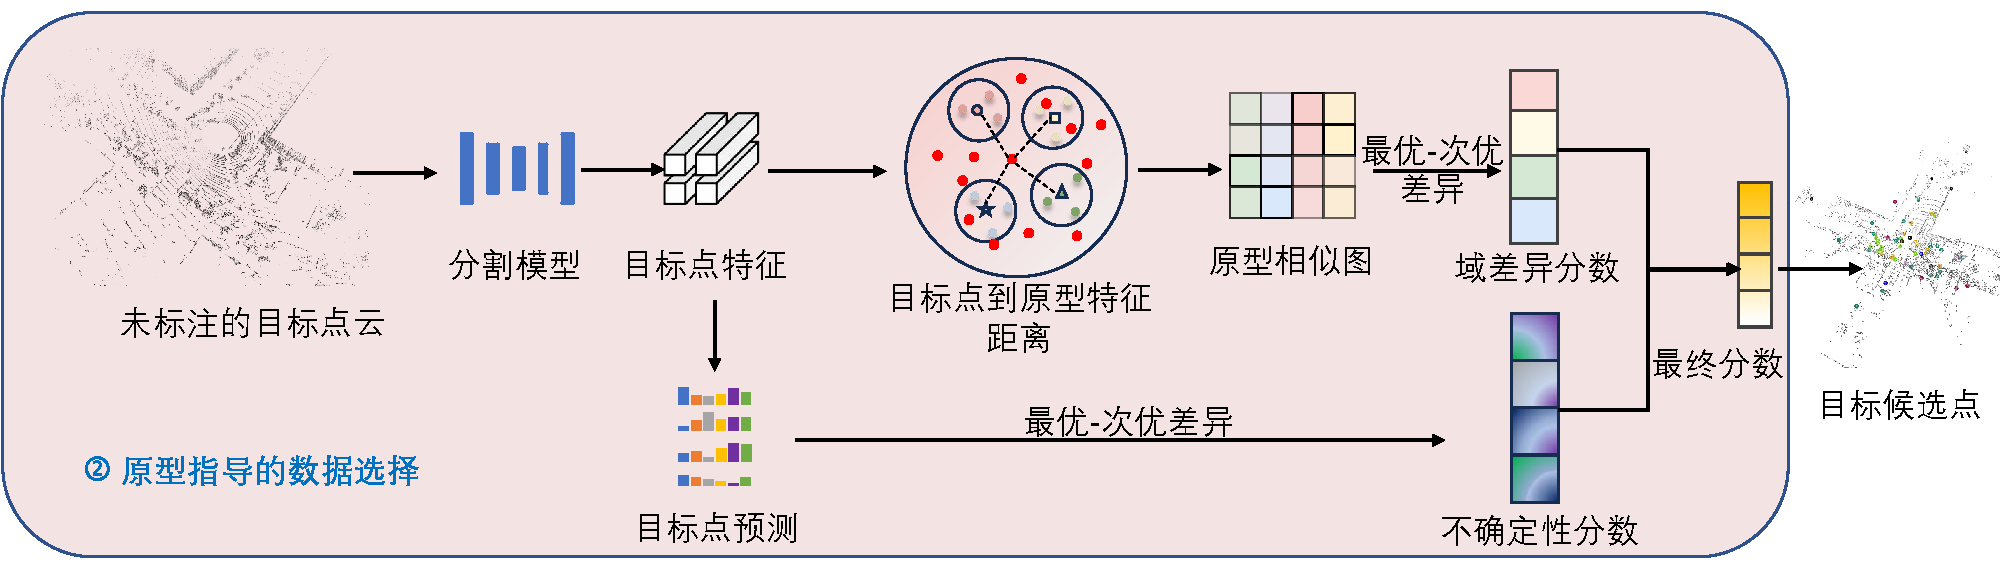
\includegraphics[width = \textwidth]{ljx/figure/3-3.pdf}
    \bicaption[\xiaosi 源域原型指导的数据选择]{\wuhao 源域原型指导的数据选择}{\wuhao Source-Prototype guided data selection}
    \label{fig:3-3}
\end{figure}
\vspace{-0.35cm}
\subsubsection{计算域差异评分}
对每个目标点\(i\)遍历计算与所有类别原型的特征距离,生成距离向量\( \mathbf{D}_i = [d_i^1, d_i^2, \dots, d_i^C] \)。为量化其域间分布特性,需将距离向量转换为相似性度量并进行归一化处理:

1)相似性转换:对\( \mathbf{D}_i\)逐元素取倒数,得到相似性向量\( \mathbf{D'}_i = [1/d_i^1, 1/d_i^2, \dots, 1/d_i^C] \),使得距离越近的类别相似度值越高。

2)概率归一化:通过Softmax函数\(f(\cdot)\)将\(\mathbf{D'}_i\)映射为概率分布,如公式\eqref{eq:softmax}所示,消除量纲差异增强判别性,确保不同类别的距离在同一尺度下比较。
% 完整公式环境示例
\begin{equation}
    \label{eq:softmax}
    f(\mathbf{D}_i') = \text{softmax}(\mathbf{D}_i') = 
    \begin{bmatrix}
    \displaystyle
    \frac{e^{d_i^{1'}}}{\sum_{c=1}^{C} e^{d_i^{c'}}}, &
    \cdots, &
    \displaystyle
    \frac{e^{d_i^{C'}}}{\sum_{c=1}^{C} e^{d_i^{c'}}}
    \end{bmatrix}
\end{equation}
最终通过最优-次优差异算法计算域差异评分\(M^i_{ds}\),公式如\eqref{eq:dis_score}所示:
\begin{equation}
    \label{eq:dis_score}
    M^i_{ds} = S_{R1}(f(\mathbf{D}_i')) - S_{R2}(f(\mathbf{D}_i'))
\end{equation}
其中\(S_{R1}(\cdot)\)和\(S_{R2}(\cdot)\)分别表示最大概率值与次大概率值。\(M^i_{ds}\)越小,则表明目标点与两个源域类别的相似度接近,意味着其处于源域类别边界区域,这样的目标点对缓解域偏移具有更高价值。

\subsubsection{融合不确定性评分}
计算得到域差异评分后,为了避免选择的点都是同类别的点,融合不确定性评分进行最终筛选。通过分割头\(h(\cdot)\)获取目标点的预测概率分布\(\mathbf{p}^t_i \in \mathbb{R}^{1\times C}\),并计算其不确定性评分\( M^i_{us} \),其表达公式如公式\eqref{eq:unc_score}所示:
\begin{equation}
    \label{eq:unc_score}
    M^i_{us} = S_{R1}(\mathbf{p}_i^t) - S_{R2}(\mathbf{p}_i^t)
\end{equation}
该评分反映模型对目标点类别判定的置信度:当最大概率与次大概率差值较小时(即\(M^i_{us}\)较小),表明模型对该点的预测存在较高不确定性,其位于类别边界上无法区分,此类样本的标注可有效提升模型性能。
为平衡域差异特性与模型不确定性,采用加权融合策略生成最终评分,其表达式如公式\eqref{eq:fin_score}所示:
\begin{equation}
    \label{eq:fin_score}
    M^i_{final} = \alpha \times M^i_{ds} + (1 - \alpha) \times M^i_{us}
\end{equation}
其中,\(\alpha \in [0,1]\)可调节的超参数。当\(\alpha=0.5\)时,两类评分贡献均等;当目标域与源域分布差异显著时,可增大以强化域差异指导作用,因此在不同的场景下\(\alpha\)可能会有所不同。

\subsubsection{筛选候选样本}
基于最终目标评分\(M^i_{final}\),对所有目标点进行升序排列,评分越低优先级越高,选取每帧点云中排名前\(k\)的点组成候选样本点集\(\mathcal{T}_l\)提交至专家(Oracle)进行人工标注,同时更新未标注目标数据集\(\mathcal{T}=\mathcal{T}-\mathcal{T}_l\),在下一轮的主动学习中,已标注的目标点将不参与筛选,其中\(k\)与主动学习轮数\(R\)以及标注总预算\(B\)的关系如公式\eqref{eq:3-9}所示:
\begin{equation}
    \label{eq:3-9}
    k=\frac{B}{R \times N^T}
\end{equation}

% 此策略即考虑了目标域选择时候的域差异问题,又考虑了类别冗余的问题,即通过结合域差异评分和不确定性评分,选择兼具高域差异和高不确定性的点,可以更好的泛化和提高模型。

% 增强域适应性:优先选择域差异评分高的样本,迫使模型关注源域未充分覆盖的特征区域

% 提升标注效率:不确定性评分高的样本往往包含更多信息量,标注此类样本可快速修正模型认知盲区

\subsection{动态混合中间域构建}
最后,为了进一步增强模型的泛化能力,本算法引入了Mixing混合方法。如图\ref{fig:3-4}所示,在每一轮训练中任意一帧目标点云都会随机匹配一帧源点云,并随机从源点云中选择一定比例的源点\(\mathbf{S}_{s_i}\),将这些选择后的源点与已标注的目标点\(\mathbf{T}_{a_i}\)进行混合,组成含两域信息的中间域数据\(\mathbf{I}_i=concat(\mathbf{T_{a_i}},\mathbf{S_{s_i}})\),其中\(concat(\cdot)\)代表拼接混合。这些中间域数据可以帮助模型学习到域不变特征,进一步缩减域间隙\upcite{chen2021semi,wang2023ssda3d}。

\vspace{-0.1cm}
\begin{figure}[h]
    \centering
    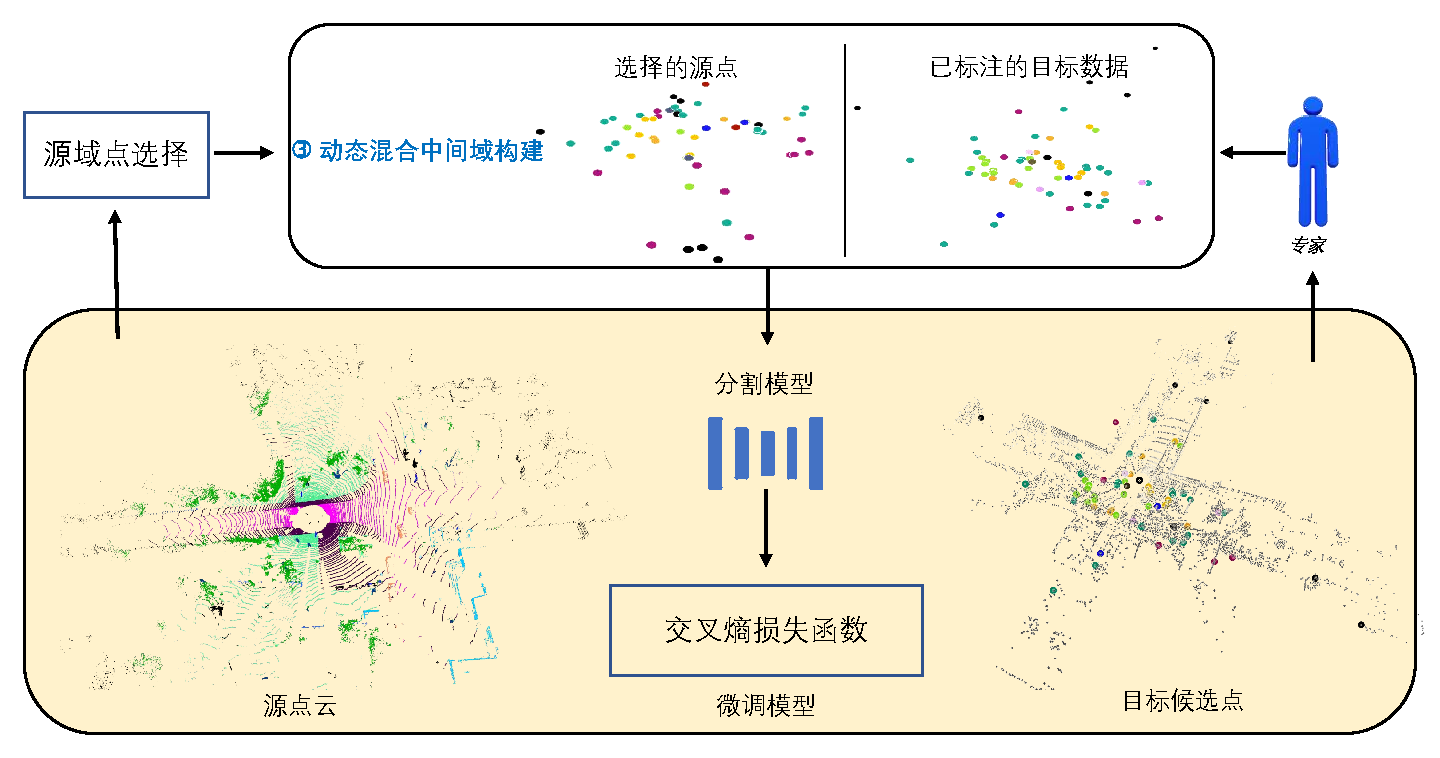
\includegraphics[width = \textwidth, scale=0.5]{ljx/figure/3-4.pdf}
    \bicaption[\xiaosi 动态混合中间域构建]{\wuhao 动态混合中间域构建}{\wuhao Dynamic mixed intermediate domain construction}
    \label{fig:3-4}
\end{figure}
\vspace{-0.35cm}
% \subsection{损失函数}放到第4章吧

\section{实验评估}
\subsection{实验设置}
在实验中,使用MinkowskiNet\upcite{MinkowskiNet}在Annotator中的PyTorch实现版本作为目标分割网络模型,并使用随机梯度下降(SGD)\upcite{SGD}作为学习优化器,动量为0.01,权重衰减系数为0.0001,在第一轮训练中使用线性预热,将学习率线性增加到基础学习率0.01,并使用初始学习率为0.01的余弦衰减调度器动态调整学习率。所有实验都在单张NVIDIA RTX A6000 GPU上进行训练。本章方法在真实到真实以及合成到真实的跨域场景下分别进行了实验。对于所有的场景,主动学习全程总共执行5次迭代并达到预设标注预算。
在合成到真实的跨域场景实验中,预训练模型(Source-only)和全监督模型(Target-only)阶段的批量大小设为16;在SynLiDAR$\to$SemanticKITTI实验中训练10轮,在SynLiDAR$\to$SemanticPOSS实验中训练20轮。而在域适应阶段,每一步的批量大小设为14并训练50轮。权重参数$\alpha$分别在SynLiDAR$\to$ SemanticKITTI和SynLiDAR$\to$SemanticPOSS的实验中设置为0.4和0.6。
在真实到真实的跨域场景实验中,SemanticKITTI$\to$nuScenes和nuScenes$\to$SemanticKITTI的实验配置相同,预训练模型Source-only和全监督模型Target-only阶段的每一步批量大小设为16,并训练10轮;在域适应阶段的每一步批量大小设置为10并训练50轮,权重参数$\alpha$为0.6。其中Mixing方法的随机混合比例为30,即混合后的中间域数据,源域点数是目标域点数的30倍。
\subsection{实验结果}
为了证明本章方法的有效性,分别在合成到真实和真实到真实这两个跨域场景下,对四个数据集进行了实验。随后,通过可视化手段对实验结果进行展示,从而更直观地呈现所提出方法在不同场景中的具体效果。
\subsubsection{合成到真实场景}
在合成到真实跨域场景的实验中,为确保与现有域适应方法的公平比较,选择SynLiDAR\(\to\)SemanticKITTI和SynLiDAR\(\to\)SemanticPOSS这两个主流的合成到真实跨域数据集进行了实验。
\vspace{0.1cm}
\begin{table}[H]
	\renewcommand{\arraystretch}{1}
    \centering
    \setlength{\tabcolsep}{10mm}
    \bicaption[\xiaosi 第三章方法与其他域适应方法在SynLiDAR\(\to\)SemanticKITTI数据上的比较]{\wuhao 本方法与其他域适应方法在SynLiDAR\(\to\)SemanticKITTI数据上的比较}{\wuhao Comparison with other domain adaptation methods on SynLiDAR\(\to\)SemanticKITTI}
    \label{tab:3-1}
    \wuhao
    \begin{tabular}{cccc}
        \toprule[1.5pt]
        \textbf{方法} & \textbf{域适应} & \textbf{标注} & \textbf{mIoU(\%)} \\
        \midrule
        Source-Only   & -          & -       & 22.8 \\
        Target-Only   & -          & 100\%       & 60.1 \\
        % AADA          & UDA & -       & 23.0 \\
        % AdvEnt        & UDA & -       & 25.8 \\
        % CRST          & UDA & -       & 26.5 \\
        % ST-PCt        & UDA & -       & 28.9 \\
        % PolarMix      & UDA & -       & 32.2 \\
        % CoSMix        & UDA & -       & 31.0 \\
        % DGT-ST        & UDA & -       & 43.1 \\
        AADA\upcite{AADA}          & UDA & -       & 23.0 \\
        AdvEnt\upcite{vu2019advent}        & UDA & -       & 25.8 \\
        CRST\upcite{zou2019confidence}          & UDA & -       & 26.5 \\
        ST-PCT\upcite{xiao2022transfer}        & UDA & -       & 28.9 \\
        PolarMix\upcite{xiao2022polarmix}      & UDA & -       & 32.2 \\
        CoSMix\upcite{saltori2022cosmix}        & UDA & -       & 31.0 \\
        DGT-ST\upcite{yuan2024density}        & UDA & -       & 43.1 \\
        % MME           & SSDA & 0.04\%  & 24.5 \\
        % APE           & SSDA & 0.04\%  & 25.1 \\
        % APE-PCT       & SSDA & 0.04\%  & 27.0 \\
        % CoSMix-SSDA   & SSDA & 0.04\%  & 34.3 \\
        % 本章方法       & SSDA   & 0.04\%   & 50.5 \\
        Annotator\upcite{Annotator}     & ADA   & 0.1\%     & 57.7 \\
        \textbf{本章方法}       & ADA   & 0.1\%     & \textbf{58.7} \\
        \bottomrule[1.5pt]
    \end{tabular}
\end{table}

实验SynLiDAR\(\to\)SemanticKITTI的结果如表\ref{tab:3-1}所示:实验结果表明,在全监督基准测试中,Source-Only模型与Target-Only模型间的性能差达到37.3个百分点,直观的反映了合成数据与真实场景间的域间分布差异,表明直接迁移模型到目标域会因为域偏移而导致严重的性能下降。在无监督域适应(UDA)的方法中,各方法性能分布在22.8\%至43.1\%区间,其中DGT-ST方法以43.1\%取得最高结果,但相较目标域全监督性能仍存在17个百分点的差距。
% 而在半监督域适应(SSDA)方法中,CoSMix-SSDA较其无监督版本提升$3.3$个百分点,说明真实标注相对无标注的有效性,而本章提出的方法达到了$50.5\%$的性能,超越了CoSMix-SSDA并实现$16.2$个百分点的提升。
在三维语义分割主动域适应(ADA)方法中,Annotator是唯一可比较的方法,为保证公平比较,主动学习预算参考其设置为0.1\%,Annotator与本章ADA方法的性能分别达到目标域全监督基准的96\%与97.7\%,证明本章方法有效性的同时也表明了主动学习域适应的高效性。提供本数据集下分割可视化如图\ref{fig:3-v-1}所示:
\vspace{-0.1cm}
\begin{figure}[H]
    \centering
    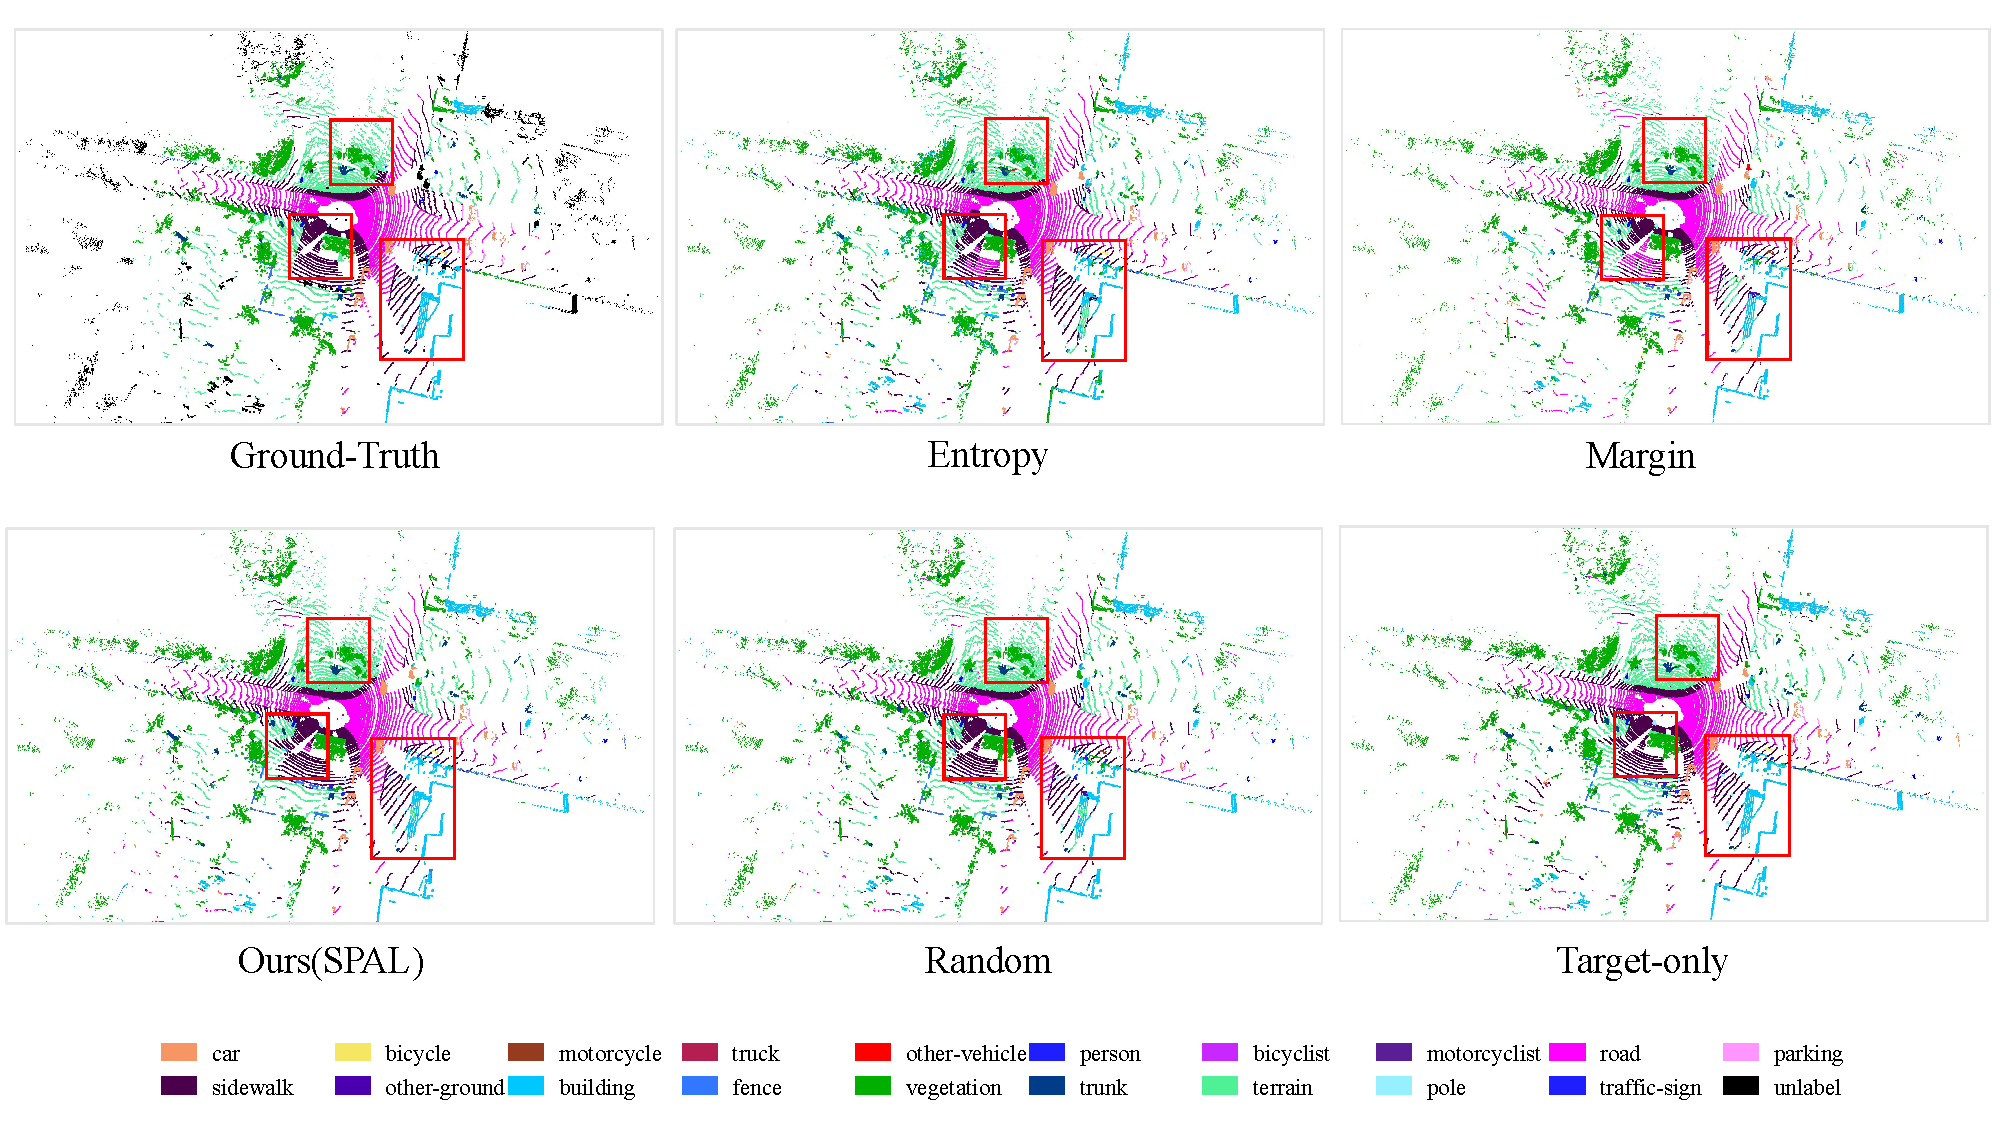
\includegraphics[width = \textwidth]{ljx/figure/3_vision_s2k1.pdf}
    \bicaption[\xiaosi 第三章SynLiDAR$\to$SemanticKITTI分割可视化图]{\wuhao 本章SynLiDAR$\to$SemanticKITTI分割可视化图}{\wuhao Visualization of the segmentation results in the SynLiDAR$\to$SemanticKITTI}
    \label{fig:3-v-1}
\end{figure}
\vspace{-0.35cm}
\vspace{0.1cm}
% \begin{table}[htbp]
\begin{table}[H]
	\renewcommand{\arraystretch}{1}
    \centering
    \setlength{\tabcolsep}{10mm}
    \bicaption[\xiaosi 第三章方法与其他域适应方法在SynLiDAR\(\to\)SemanticPOSS数据上的比较]{\wuhao 本方法与其他域适应方法在SynLiDAR\(\to\)SemanticPOSS数据上的比较}{\wuhao Comparison with other domain adaptation methods on SynLiDAR\(\to\)SemanticPOSS}
    \label{tab:3-2}
    \wuhao
    \begin{tabular}{cccc}
        \toprule[1.5pt]
        \textbf{方法} & \textbf{域适应} & \textbf{标注} & \textbf{mIoU(\%)} \\
        \midrule
        Source-Only   & -           & -       & 34.6 \\
        Target-Only   & -           & 100\%       & 58.0 \\
        % CRST          & UDA & -       & 27.1 \\
        % ST-PCT        & UDA & -       & 29.6 \\
        % PolarMix      & UDA & -       & 30.4 \\
        % CoSMix        & UDA & -       & 40.4 \\
        % DGT-ST        & UDA & -       & 50.8 \\
        CRST\upcite{zou2019confidence}          & UDA & -       & 27.1 \\
        ST-PCT\upcite{xiao2022transfer}        & UDA & -       & 29.6 \\
        PolarMix\upcite{xiao2022polarmix}      & UDA & -       & 30.4 \\
        CoSMix\upcite{saltori2022cosmix}        & UDA & -       & 40.4 \\
        DGT-ST\upcite{yuan2024density}        & UDA & -       & 50.8 \\
        % MME           & SSDA & 0.01\%  & 33.2 \\
        % APE           & SSDA & 0.01\%  & 30.3 \\
        % APE-PCT       & SSDA & 0.01\%  & 31.2 \\
        % CoSMix-SSDA   & SSDA & 0.01\%  & 41.0 \\
        % 本章方法       & SSDA   & 0.01\%   & 57.5 \\
        Annotator\upcite{Annotator}     & ADA   & 0.1\%     & 52.0 \\
        \textbf{本章方法}       & ADA   & 0.1\%     & \textbf{56.6} \\
        \bottomrule[1.5pt]
    \end{tabular}
\end{table}
实验SynLiDAR\(\to\)SemanticKITTI的结果如表\ref{tab:3-2}所示:在无监督域适应(UDA)方法中,DGT-ST仍以50.8\%的性能占据首位;
% 而在半监督域适应(SSDA)方法中,本章方法在$0.01\%$极少量标注下达到$57.5\%$逼近全监督目标域性能,同时超过CoSMix$16.5$个百分点;
而在主动域适应(ADA)方法中,本章方法在0.1\%的标注下取得56.6\%的性能超过Annotator4.6个百分点,再一次证明了本章方法在合成到真实的跨域场景的有效性。可视化结果如图\ref{fig:3-v-2}所示:

\vspace{-0.1cm}
\begin{figure}[H]
    \centering
    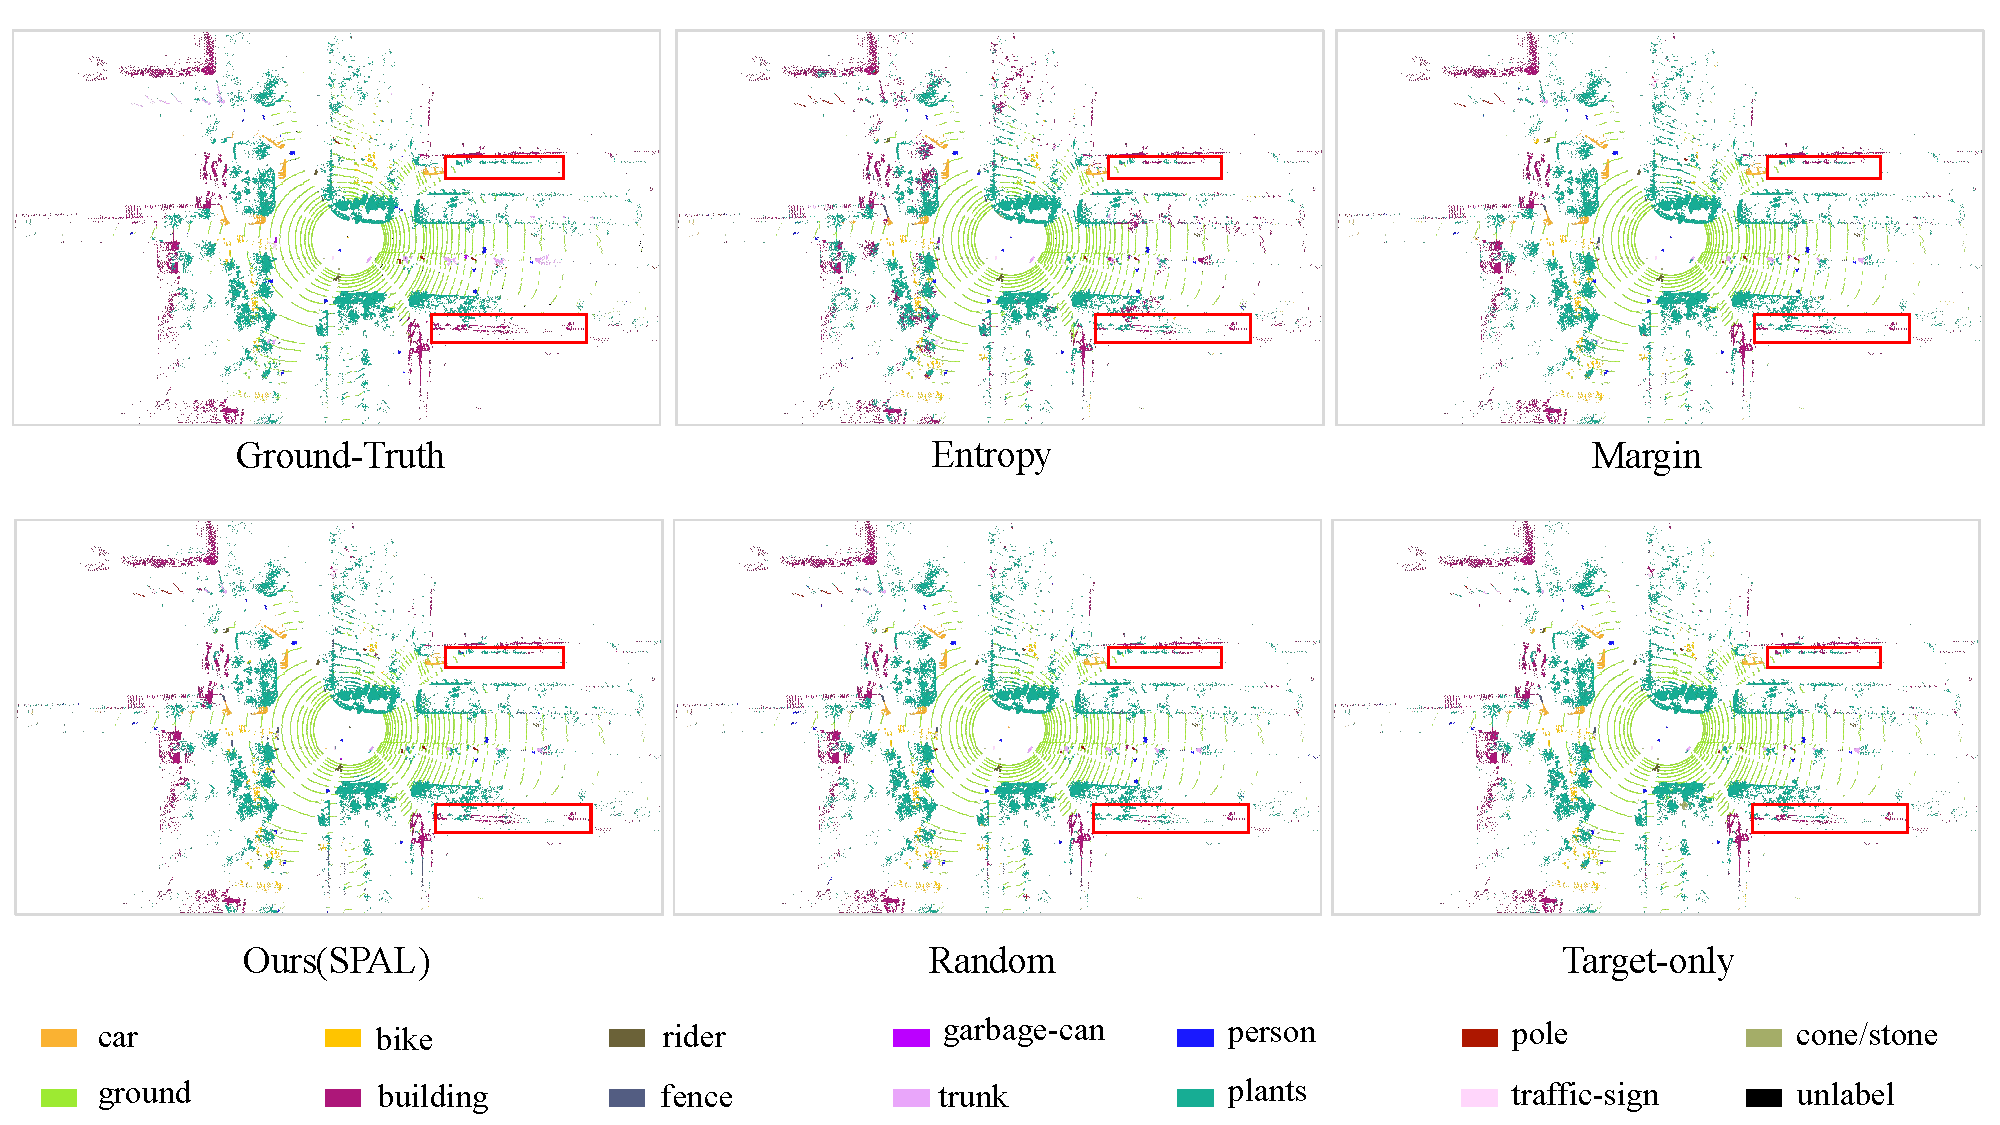
\includegraphics[width = \textwidth]{ljx/figure/3_vision_s2p.pdf}
    \bicaption[\xiaosi 第三章SynLiDAR$\to$SemanticPOSS分割可视化图]{\wuhao 本章SynLiDAR$\to$SemanticPOSS分割可视化图}{\wuhao Visualization of the segmentation results in the SynLiDAR$\to$SemanticPOSS}
    \label{fig:3-v-2}
\end{figure}
\vspace{-0.35cm}

\subsubsection{真实到真实场景}
在合成到真实的跨域任务中,合成的数据集一般都有着标注精度更高,噪音度低的特性,其仍然与真实数据集有所差异。为进一步验证方法的泛化能力,本章将方法拓展至“真实到真实”跨域场景,并选择nuScenes\(\to\)SemanticKITTI和SemanticKITTI\(\to\)nuScenes跨域数据集进行了实验,在此场景下,本章方法展现出与合成到真实任务相似的性能优势,进一步证明了本章方法的有效性。

如表\ref{tab:3-3}所示,在SemanticKITTI$\to$nuScenes实验中,目标域全监督基准结果与源域模型间存在49.0个百分点的性能差距,这说明在真实数据间,跨域任务要比合成更难。无监督域适应(UDA)方法中,LiDOG以34.9\%领先,但其性能仅为目标域基准的42.2\%,说明了无监督域适应在真实场景中的局限性,虽然不用进行标记但其性能仍然离全监督非常远。而本章ADA方法以0.1\%标注量达到目标域全监督的97.9\%,较Annotator提升5.1个百分点,验证了本方法的有效性。同合成到真实数据集一样,本实验依然提供与Ground-Truth、Target-Only以及其他主动学习的可视化对比图,如图\ref{fig:3-v-3}所示:
\vspace{0.1cm}
% \begin{table}[htbp]
\begin{table}[H]
	\renewcommand{\arraystretch}{1}
    \centering
    \setlength{\tabcolsep}{12mm}
    \bicaption[\xiaosi 第三章方法与其他域适应方法在SemanticKITTI\(\to\)nuScenes数据上的比较]{\wuhao 本方法与其他域适应方法在SemanticKITTI\(\to\)nuScenes数据上的比较}{\wuhao Comparison with other domain adaptation methods on SemanticKITTI\(\to\)nuScenes}
    \label{tab:3-3}
    \wuhao
    \begin{tabular}{lccc}
        \toprule[1.5pt]
        \textbf{方法} & \textbf{域适应} & \textbf{标注} & \textbf{结果} \\
        \midrule
        Source-Only   & -       & -           & 33.7 \\
        Target-Only   & -       & 100\%           & 82.7 \\
        Mix3D         & UDA     & -   & 31.5 \\
        CoSMix        & UDA     & -   & 29.8 \\
        SN              & UDA   & -     & 25.8 \\
        RayCast        & UDA    & -    & 30.9 \\
        LiDOG        & UDA      & -       & 34.9 \\
        Annotator     & ADA     & 0.1\%     & 75.9 \\
        本章方法       & ADA    & 0.1\%      & \textbf{81.0(改)} \\
        \bottomrule[1.5pt]
    \end{tabular}
\end{table}

\vspace{-0.1cm}
\begin{figure}[h]
    \centering
    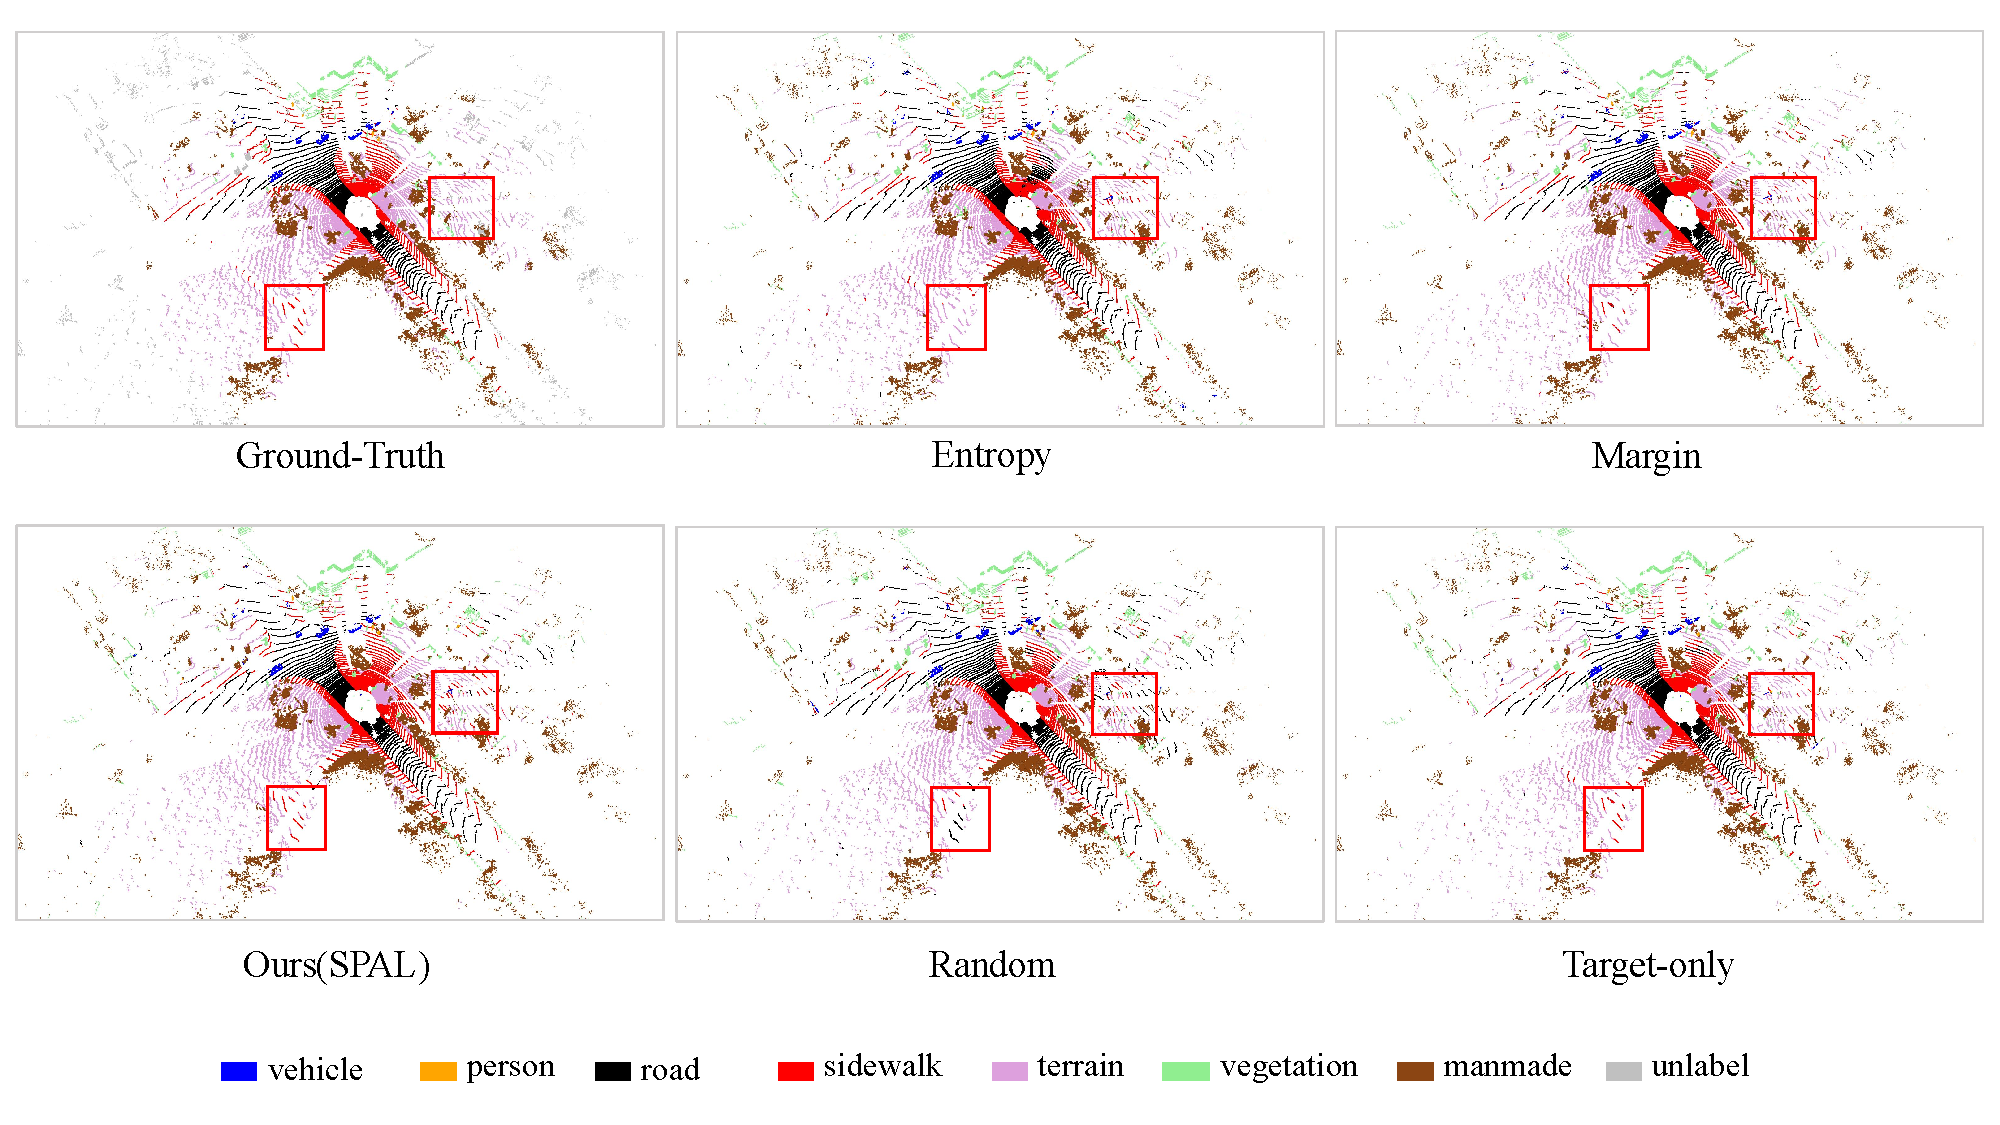
\includegraphics[width = \textwidth]{ljx/figure/3_vision_k2n.pdf}
    \bicaption[\xiaosi 第三章SemanticKITTI$\to$nuScenes分割可视化图]{\wuhao 本章nuScenes$\to$SemanticKITTI分割可视化图}{\wuhao Visualization of the segmentation results in the SemanticKITTI$\to$nuScenes}
    \label{fig:3-v-3}
\end{figure}
\vspace{-0.35cm}
在nuScenes→SemanticKITTI中如表\ref{tab:3-4}所示,目标域全监督性能与源域差距进一步扩大至52.9个百分点,任务难度进一步增加。值得注意的是,本章ADA方法在0.1\%标注下完全复现目标域全监督性能,较Annotator提升3.6个百分点,首次实现极低标注量下的无损迁移。对比两类场景,UDA方法LiDOG在nuScenes\(\to\)SemanticKITTI任务中的性能依然强势,但是仍距离全监督有接近44.2个百分点的性能差距。综合而言,本章方法在真实到真实场景中均以0.1\%标注量实现超95\%全监督性能。可视化结果如图\ref{fig:3-v-4}所示:
\vspace{0.1cm}
% \begin{table}[htbp]
\begin{table}[H]
	\renewcommand{\arraystretch}{1}
    \centering
    \setlength{\tabcolsep}{12mm}
    \bicaption[\xiaosi 第三章方法与其他域适应方法在nuScenes\(\to\)SemanticKITTI数据上的比较]{\wuhao 本方法与其他域适应方法在nuScenes\(\to\)SemanticKITTI数据上的比较}{\wuhao Comparison with other domain adaptation methods on nuScenes\(\to\)SemanticKITTI}
    \label{tab:3-4}
    \wuhao
    \begin{tabular}{lccc}
        \toprule[1.5pt]
        \textbf{方法} & \textbf{域适应} & \textbf{标注} \textbf{结果} \\
        \midrule
        Target-Only   & -       & 100\%           & 85.4 \\
        Source-Only   & -       & -           & 32.5 \\
        Mix3D         & UDA     & -   & 32.4 \\
        CoSMix        & UDA     & -   & 36.8 \\
        SN              & UDA   & -     & 23.6 \\
        RayCast        & UDA    & -    & 31.5 \\
        LiDOG        & UDA      & -       & 41.2 \\
        Annotator     & ADA     & 0.1\%     & 81.8 \\
        本章方法       & ADA    & 0.1\%      & \textbf{85.4(改)} \\
        \bottomrule[1.5pt]
    \end{tabular}
\end{table}

\vspace{-0.1cm}
% \begin{figure}[h]
\begin{figure}[H]
    \centering
    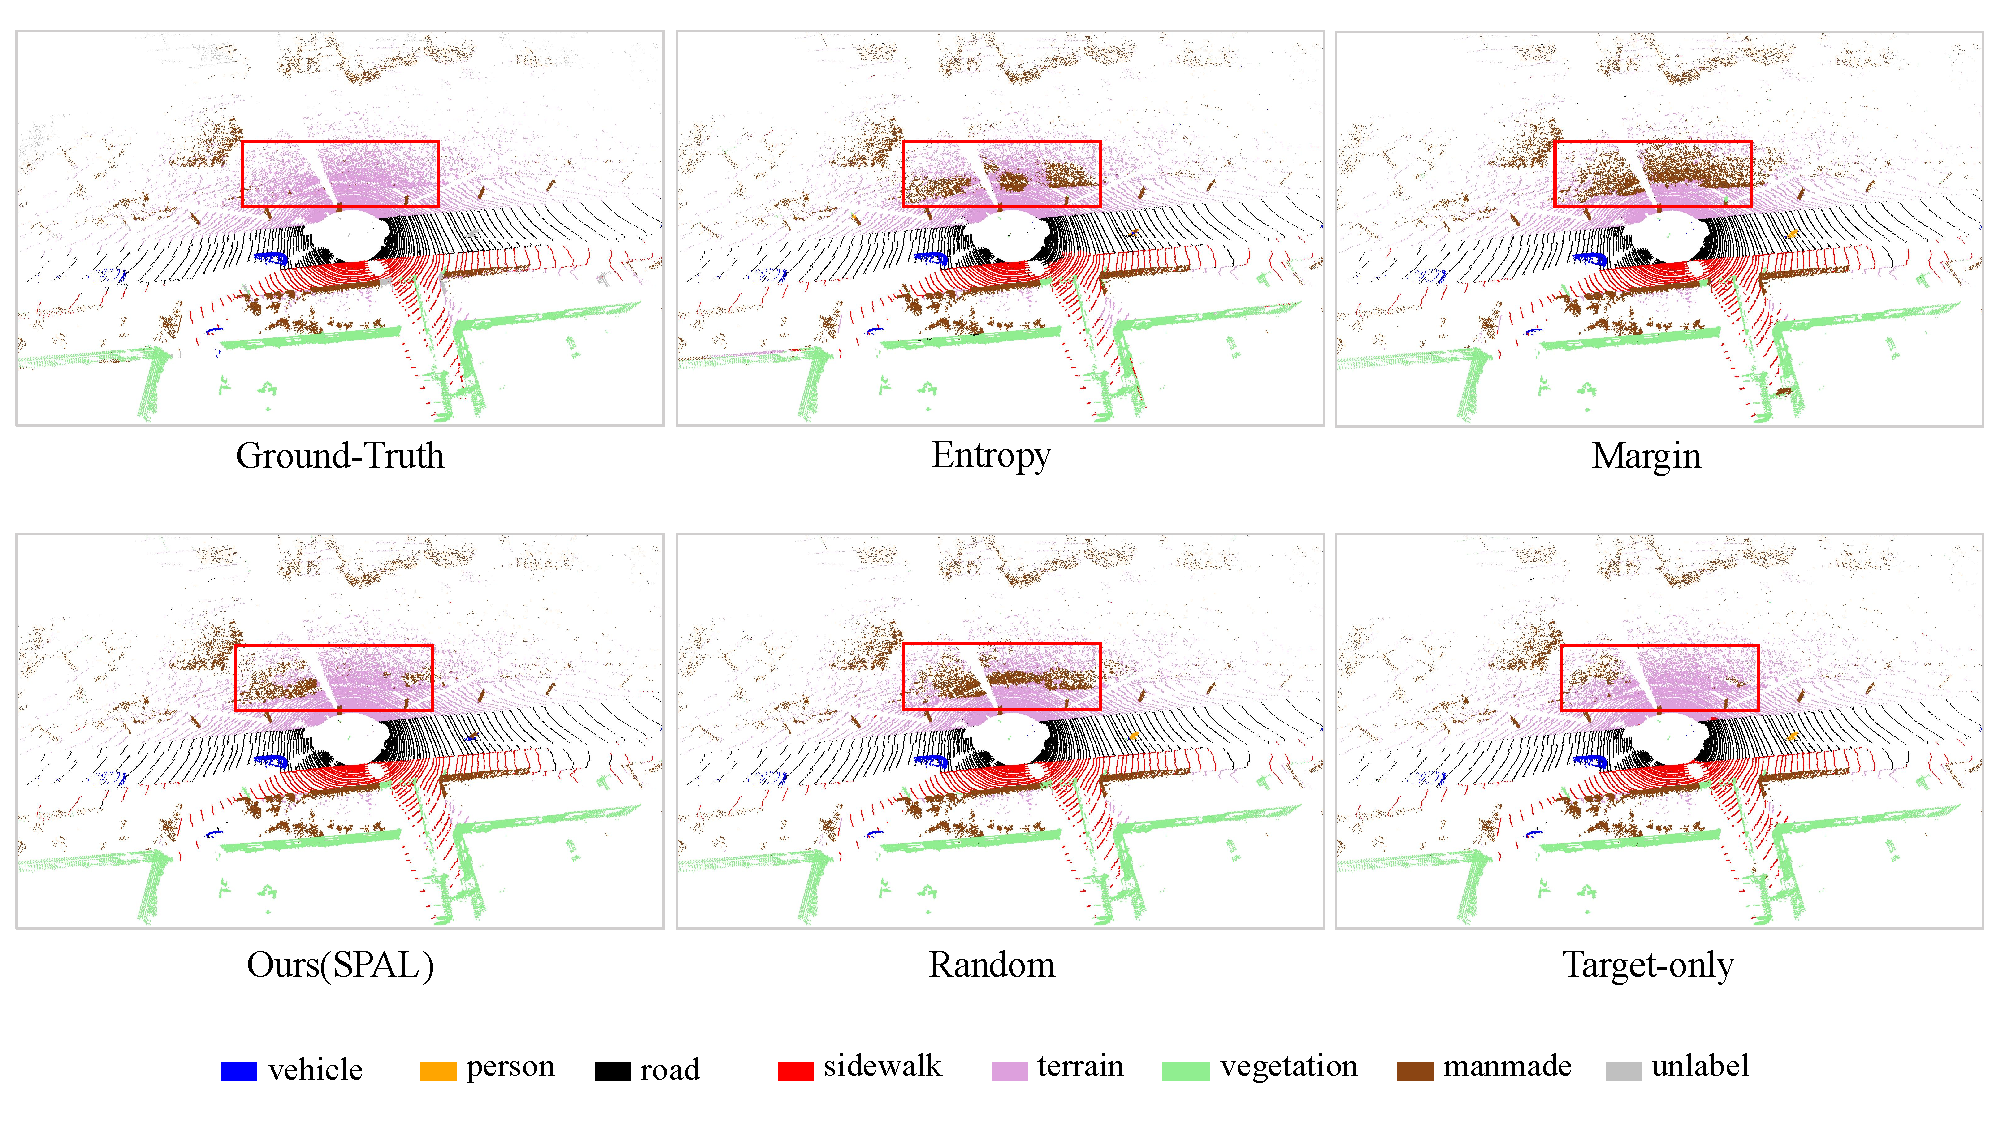
\includegraphics[width = \textwidth]{ljx/figure/3_vision_n2k.pdf}
    \bicaption[\xiaosi 第三章nuScenes$\to$SemanticKITTI分割可视化图]{\wuhao 本章nuScenes$\to$SemanticKITTI分割可视化图}{\wuhao Visualization of the segmentation results in the nuScenes$\to$SemanticKITTI}
    \label{fig:3-v-4}
\end{figure}
\vspace{-0.35cm}
\subsection{消融对比实验}
\subsubsection{与其他主动学习方法对比}
在未引入Mixing策略时,传统主动学习方法在两类合成到真实跨域任务中表现出了一定的优势如表\ref{tab:3-5}所示。本章的方法是通过源域而构建起的原型,因此比较依赖源域信息,在没有mixing的情况下无法发挥最大的效果,在SynLiDAR$\to$SemanticKITTI任务中,Margin方法以54.4\%的性能取得最优结果,而本章方法(SPAL)以53.5\%略低1.1个百分点,但仍然超过了Random0.2个百分点Entropy2.8个百分点。
而在SynLiDAR$\to$SemanticPOSS任务中,本章的主动学习策略(SPAL)低于熵采样(Entropy)0.7个百分点,却也超过了Random3.2个百分点,Margin0.2个百分点,这一结果表明,传统主动学习策略在特定场景下仍具竞争力,但单一采样准则难以适应跨域任务的复杂性。
\vspace{0.1cm}
% \begin{table}[htbp]
\begin{table}[H]
	\renewcommand{\arraystretch}{1}
    \centering
    \setlength{\tabcolsep}{10mm}
    \bicaption[\xiaosi 第三章主动学习方法与其他传统主动学习方法对比]{\wuhao 本章的主动学习方法与其他传统主动学习方法对比}{\wuhao  Comparison with other active learning methods}
    \label{tab:3-5}
    \wuhao
    \begin{tabular}{cccc}
        \toprule[1.5pt]
        \textbf{数据集} & \textbf{方法} & \textbf{标注} & \textbf{结果} \\
        \midrule
        \multirow{4}{*}{SynLiDAR\(\to\)SemanticKITTI} & 
        Random              & 0.1\%        & 53.2 \\
        ~ & Entropy\upcite{Entropy}             & 0.1\%        & 51.7 \\
        ~ & \textbf{Margin}\upcite{Margin}              & 0.1\%        & \textbf{54.4} \\
        ~ & Ours(SPAL)          & 0.1\%        & 53.5 \\
        \multirow{4}{*}{SynLiDAR\(\to\)SemanticPOSS} & 
        Random              & 0.1\%        & 47.5 \\
        ~ & \textbf{Entropy}\upcite{Entropy}             & 0.1\%        & \textbf{51.4} \\
        ~ & Margin\upcite{Margin}              & 0.1\%        & 50.5 \\
        ~ & Ours(SPAL)          & 0.1\%        & 50.7 \\
        \bottomrule[1.5pt]
    \end{tabular}
\end{table}

而在结合Mixing策略后如表\ref{tab:3-6}所示,除Random以外各主动学习方法在SynLiDAR$\to$SemanticKITTI任务中的性能均显著提升,其中本章方法(SPAL)以58.7\%的性能达到最优,较次优的Margin方法提升1.1个百分点,较未结合Mixing时的自身结果提升5.2个百分点且显著超越传统方法Margin的57.6\%,Margin、Entropy则分别较自身提升3.2和3.4个百分点。这表明结合主动学习和Mixing策略的有效性,通过主动筛选出的标注目标点和源点动态构建中间域数据可以有效提升模型的性能,进一步缓解域间分布差异。但Random方法下降了2.1个百分点,这说明性能增益也与主动学习方法有关系,混合中间域信息包含域差异信息越丰富,其提升程度越高,而本文方法差异选择的是差异性和不确定性最高的点,因此提升幅度最大。
\vspace{0.1cm}
% \begin{table}[htbp]
\begin{table}[H]
	\renewcommand{\arraystretch}{1}
    \centering
    \setlength{\tabcolsep}{10mm}
    \bicaption[\xiaosi 第三章主动学习方法与其他传统主动学习方法在结合Mixing后的对比]{\wuhao 本章主动学习方法与其他传统主动学习方法在结合Mixing后的对比}{\wuhao  Comparison with other active learning methods after integrating Mixing}
    \label{tab:3-6}
    \wuhao
    \begin{tabular}{cccc}
        \toprule[1.5pt]
        \textbf{数据集} & \textbf{方法} & \textbf{标注} & \textbf{结果} \\
        \midrule
        \multirow{4}{*}{SynLiDAR\(\to\)SemanticKITTI}
        & Random              & 0.1\%        & 51.1 \\
        ~ & Entropy\upcite{Entropy}             & 0.1\%        & 55.1 \\
        ~ & Margin\upcite{Margin}              & 0.1\%        & 57.6 \\
        ~ & \textbf{Ours(SPAL)}          & 0.1\%        & \textbf{58.7} \\
        \bottomrule[1.5pt]
    \end{tabular}
\end{table}

\subsubsection{消融实验}
为证明方法的有效性,本章在SynLiDAR$\to$SemanticKITTI数据上进行了消融实验,结果如表\ref{tab:3-7}所示,本章提出的源域指导的主动学习方法(SPAL)与混合增强(Mixing)策略构建的中间域数据对模型性能具有显著协同优化作用。仅使用SPAL时,模型性能提升至50.7\%,较基线增加27.9个百分点,证明了原型指导的数据选择主动学习方法对目标域关键样本筛选的优势。而当仅使用Mixing,模型性能为51.2\%,较无任何模块的基线提升28.3个百分点,验证了跨域数据融合对缓解域间分布差异的有效性。而当二者联合使用时,模型以58.7\%的结果达到最优,较单一模块性能分别提升8.0和7.5个百分点,表明本章方法的真实有效性。
\vspace{0.1cm}
% \begin{table}[htbp]
% 	\renewcommand{\arraystretch}{1}
%     \centering
%     \setlength{\tabcolsep}{2mm}
%     \bicaption[\xiaosi 第三章方法与先进方法关于内点率的比较]{\wuhao 本方法与先进方法关于内点率的比较}{\wuhao Comparison of Inlier Ratio between this method and advanced methods}
%     \label{tab:3-7}
%     \wuhao
%     \begin{tabular}{lccc}
%         \toprule[1.5pt]
%         \textbf{方法} & \textbf{主动学习(SPAL)} & \textbf{Mixing} & \textbf{结果} \\
%         \midrule
%         \multirow{4}{*}{SynLiDAR\(\to\)SemanticKITTI} &
%           &            &           22.8\\
%         ~ &      \checkmark &         & 50.7 \\
%         ~ &              &  \checkmark        & running... \\
%         ~ & \checkmark          & \checkmark        & \textbf{58.7} \\
%         \bottomrule[1.5pt]
%     \end{tabular}
% \end{table}

% \begin{table}[htbp]
\begin{table}[H]
	\renewcommand{\arraystretch}{1}
    \centering
    \setlength{\tabcolsep}{10mm}
    \bicaption[\xiaosi 第三章方法消融实验]{\wuhao 本章方法模块消融实验}{\wuhao Ablation experiments on modules}
    \label{tab:3-7}
    \wuhao
    \begin{tabular}{ccc}
        \toprule[1.5pt]
        \textbf{主动学习(SPAL)} & \textbf{Mixing} & \textbf{结果} \\
        \midrule
          &             &                   22.8\\
        \checkmark      &               &   50.7 \\
                        &  \checkmark        & 51.2 \\
         \checkmark          & \checkmark        & \textbf{58.7} \\
        \bottomrule[1.5pt]
    \end{tabular}
\end{table}

\section{本章小结}
本章主要研究适用于点云语义分割域适应任务的主动学习方法。为了解决传统主动学习方法中的不足,提出了一种原型指导的主动学习策略,该策略通过动态构建源域原型来代表源域类别质心,并在每一轮主动学习阶段实时更新原型,在进行目标域候选点筛选时,计算每个目标域中未标注的点与每个源域类别原型的相似度,通过最优-次优差异算法获取归一化后的类别概率的差值得到域差异性评分,值越小说明该点域差异性越高,同时结合不确定性评分得到最终候选评分,升序排列后选取前k个同时兼备高不确定性和高域差异性的目标点。此外,本章首次将主动学习方法与Mixing策略结合,构建包含目标域信息和源域信息的中间域数据,帮助模型学习到更稳定的域不变特征,进一步缩小域间隙。在本章中,首先介绍了方法的主要框架和流程,并分别对方法中的三个模块做了详细介绍,这三个模块共同组成了本章的方法,大幅度提升了模型的跨域性能。同时, 为了验证方法的有效性,在两个跨域场景四个数据集上进行了大量实验,并与此前最有效的点云语义分割无监督域适应和主动域适应进行了对比,通过实验分析验证了本章方法的有效性,最后进一步对Mixing和SPAL模块进行消融实验,充分验证了两个模块的有效性。

% 验证AL与mix的有效性
% 验证不同参数下的结果
% 验证不同预算下的结果

% 第4章
\chapter{基于点云语义分割域适应的主动混合方法}
\thispagestyle{others}
\pagestyle{others}
\xiaosi

    \section{本章引言}
    本章主要介绍基于点云语义分割域适应的主动混合方法。该方法通过将基于原型指导的主动学习方法和本节所提出的主动混合方法进行深度结合,进一步提升了主动域适应方法的结果。接下来,下文将分别从方法提出的研究动机及主要贡献、方法的具体组成和实现细节,以及实验分析评估等方面,对所提出的方法进行全面阐述。 

    \section{研究动机及贡献}
    % 首先说研究背景和问题,再说一些解决的方法,然后提一下前者怎么做的,后者怎么做的
    % 第二就是说一些文章,他们是怎么使用这些方法解决问题的
    % 第三就是提上述文章方法的不足,
    % 核心点是:主动域适应中主动学习与mixing的结合不够深入,仍然有很大的探索空间。
    % 背景现状(标注问题)-> 一些现存的方法 -> 域适应中和主动学习以及mixing的方法 -> mixing方法构建中间域,举例一些方法,然后这些方法在mixing的不足,尽管如此,但是mixing与主动学习在域适应的结合是从没有过,或者说mixing与主动学习的结合从未有过探索,但是它们却有着巨大的探索价值 -> 我们从上一章节看到了mixing带来的提升,但是基于AL的mixing还有更大的探索空间,对于这两个的结合的探索仍然缺乏。
    % 一些研究者将mixing用于半监督域适应中
    % 主动域适应的问题,以及mixing却可以为之互补。
    % 域适应中有主动域适应和一些基于无监督或者半监督的域适应。
    % 然而在域适应中主动学习方法和mixing
    % 提及一些主动域适应的方法以及已无监督域适应的一些mixing方法
    % 在。。中,。。。使用mixing。。。的提升了模型性能,域适应中。。。使用mixing提升了性能,在。。。中通过主动域适应得到了很好的解决,mixing和主动学习分别为标注问题默默贡献着。或者直接说主动域适应的问题,然后引出一些mixing方法的好处,可以完美的进行结合。
    % 科技的进步使得点云雷达数据的获取变得更加容易,深度学习技术的发展则使得点云语义分割任务得到了快速进步,一些优秀的模型接踵而至,并取得了令人瞩目的结果。但是,这些优秀模型都是基于全监督模式下的,需要点云样本进行逐点的标注,而点云标注则是一项耗费人力物力的艰巨任务。为了缓解这以问题,一些优秀的方法被提出,而域适应就是其中之一。在无监督和半监督域适应中,一些方法独出心裁,使用mixing的方法构造中间域来学习特征的不变性,进而解决域偏差问题。polarmix[]。提出将不同的雷达线速进裁剪并混合。CoSMix[]。将指定语义类别的源域点和伪标签置信度高于阈值的目标点进行过交换混合。而主动域适应[HPML、CLUE、SDM]则是通过选择对缩减域偏差帮助最大的目标点,并进行标注后以提升模型的性能。
    科技的进步使得获取点云雷达数据变得更加容易,而深度学习技术的发展则推动了点云语义分割任务的迅速提升,涌现出一系列优秀模型并取得了显著成果。然而,这些模型大多基于全监督模式,需要对点云样本进行逐点标注,这是一项耗费大量人力物力的艰巨任务。为缓解这一问题,研究者们提出了多种方法,而域适应就是其中一种有效的策略。在无监督和半监督域适应中,一些方法巧妙地使用混合(Mixing)方法构建中间域,以学习域不变特征,进而解决域偏差问题。Polarmix\upcite{xiao2022polarmix}方法
    % 是沿方位角分割
    在$x,y$组成的水平面上,按照指定的角度分割
    并混合不同扫描区域的点云数据,在域适应中混合的则是不同数据集下的同角度点云区域。LaserMix\upcite{kong2023lasermix}方法则是沿方位角,裁剪并混合不同点云中相同角度的雷达线束,在域适应中混合的则是不同数据集下相同线束点云。
    % CoSMix\upcite{saltori2022cosmix}方法则交换并混合源域中指定语义类别的点与目标域中伪标签置信度高于阈值的点。
    此外,主动域适应方法\upcite{CLUE,HPML,SDM}通过主动选择对减小域偏差最有帮助的目标点进行标注,从而提升模型性能。 

    尽管上述算法各自以不同方式缓解了标注问题,提升了分割模型的性能,但在域适应中,主动学习与Mixing方法的结合尚未得到深入研究。无论是在图像还是三维点云领域,混合方法和主动学习通常独立应用,分别为减少标注需求做出贡献。然而,现有的混合方法若直接应用于主动域适应,可能存在以下问题:1)数量不均衡导致的域偏差问题。现有的混合方法多基于同一数据集或大量伪标签,特点是场景连续且点数丰富。然而在域适应中,源域和目标域存在域偏移,主动学习预算下选择的点数量有限。若直接应用这些混合方法,可能导致模型过度学习源域信息,阻碍对目标域信息的提取,最终导致次优结果。因此,在主动域适应中,保持源域和目标域信息的平衡可能比场景连续性更为重要。2)主动学习选点导致的语义类别不平衡问题。大多数主动学习选点策略基于不确定性,在实际标注前,无法确定所选子集的类别分布是否均衡。尽管一些方法通过伪标签预判类别,但这基于模型不可靠的预测,在域适应任务中可能不适用。此外,现有的混合方法未考虑逐点的语义类别平衡问题。因此,如何使主动学习选择的目标子集与源数据混合后的训练子集在类别分布上尽可能平衡,仍是一个普遍存在的问题。
    针对上述问题,本章进一步探讨了主动学习方法与混合方法在域适应任务中的深度结合。在该方法中,延续前章使用基于原型指导的主动学习与Mixing相结合的基础框架。在此基础上,提出了面向点云语义分割域适应的主动混合方法。其包括两个模块:源-目标数量平衡模块旨在解决数量不均衡导致的域偏差问题;类别平衡主动混合模块用于解决主动学习选点导致的语义类别不平衡问题。这两个模块有效地实现了主动学习与Mixing方法的深度结合,进一步提升了模型的分割性能。
    % 虽然上述算法都通过自己的方式解决了标注问题,使得分割模型有了一定的提升,但是对于域适应中主动学习和mixing的结合并未有人进行过深入的探索,无论是在图像还是三维点云领域,mixing和主动学习独立且分别为缓解标注问题默默贡献着。而现存的mixing方法如果直接运用到主动域适应中可能存在以下问题:1)数量不均衡而导致域偏差问题,由于之间的mixing方法更多的是基于同一数据集或者大量的伪标签的前提下的,因此这些方法有着共同的特点:场景连续且点数更多。而在域适应中,目标域和源域之间存在域偏移问题,并且主动学习预算选择的点非常少,因此如果直接将这些mixing方法运用到主动域适应中,可能会导致模型因学习到更多源域信息而阻碍对目标域信息的提取,得到次优的模型结果。因此在主动域适中,场景的连续可能并不是那么重要,相同的源-目标域信息可能才是进一步提升模型性能的最佳混合方法。2)主动学习选点导致的语义类别不平衡问题。目前为止,大多数主动学习的选点策略都是基于不确定性的,在真实标注之前,我们无法得知最终选择的子集的类别分布是否均衡,虽然有一些方法通过伪标签的方式提前预判选择的类别,但这仍然是基于模型的不可靠预测的伪标签,在域适应任务中可能并不适用,现有的mixing未考虑逐点即语义类别平衡的问题,因此存在一个普遍的问题,
    % 如何使得主动学习选择后的目标子集与源数据混合后的训练子集是类别分布尽可能得平衡。对于上述问题,本章节进一步探索了用于域适应任务的主动学习方法与mxing深度结合。在该方法中,首先将提出的基于原型指导的主动学习与Mixing结合形成了基础结合框架,并基于该框架提出了面向点云语义分割域适应的源-目标数量平衡算法和类别平衡主动混合算法。源-目标数量平衡算法解决数量不均衡而导致域偏差问题,类别平衡主动混合算法用于解决主动学习选点导致的语义类别不平衡问题。两个算法有效的完成了主动学习和mixing方法的深入结合,并进一步提高了模型分割的性能。
    
    本章研究的主要贡献如下:

    1)提出了源-目标数量平衡模块,通过选择与目标域样本中标注数量相同的源点进行混合构建中间域,解决了因数量不平衡导致的域偏差积累问题,进一步提高了混合中间域的有效性。

    2)提出了类别平衡主动混合模块,利用在源-目标数量平衡算法得到多个候选源点混合子集,计算并选择与标注的目标域混合后类别分布最为均衡的子集进行Mixing,借助源域数据实现主动选点的类别平衡,进一步提升了主动学习的有效性。

    3)根据提出的两个算法模块实现了主动学习与Mixing的深入结合,得到了深度融合主动混合的点云语义分割域适应框架,分割表现领先于所有现存的点云语义分割域适应方法。

    % 为了更进一步提升在主动域适应中主动学习方法与Mixing的进一步结合,提出了基于点云语义分割域适应的主动混合方法。在该方法中,首先将提出的基于原型指导的主动学习与Mixing结合形成了基础结合框架,并基于该框架提出了面向点云语义分割域适应的源-目标数量平衡算法和类别平衡主动混合算法,两个算法有效的适配了主动域适应中的主动学习,减小了域差异和主动选择中类别不平衡则一普遍存在的问题,并进一步提高了模型分割的性能。

    \section{基于点云语义分割域适应的主动混合方法}
    \subsection{方法概述}%加上后删点内容
    在第三章中,设计了一个基于原型的主动学习方法,并初步尝试结合混合方法构建强健的中间域数据,以缩减域偏差,提升模型性能。然而,混合方法与主动学习的结合仍有广阔的探索空间。如何根据域偏差以及主动学习的特点来有效结合混合方法,仍是一个值得深入研究的问题。

    为了深入探讨Mixing方法与主动学习在域适应任务中的深度融合,本章在第三章提出的总体框架基础上进行了改进,改进后的框架如图\ref{fig:4-1}所示。该算法的基本流程主要由三个主要模块构成:%\ding{172}源域原型构建模块;
    \ding{172}源原型引导的数据选择模块(SPAL);\ding{173}源-目标数量平衡模块(STNB);\ding{174}类别平衡主动混合模块(CBAM)。为进一步实现两者的高效协同作用,从而获得更优的分割表现,本章对第三章的动态中间域构建模块进行了改进,分为两个模块:一是源-目标数量平衡模块,选择类别数量大于预设定值的源域帧,并从中筛选与所匹配的目标域帧标注点数平衡的候选子集;二是类别平衡主动混合模块,计算每个候选子集与目标域帧标注点混合后的类别分布熵值,选择熵值最大的候选源域子集,以构建类别相对平衡的中间域数据。通过上述改进,实现混合方法与主动学习的深度融合,进一步提升点云语义分割模型的性能。 
    % \vspace{-0.1cm}
    \begin{figure}[H]
        \vspace{-0.1cm}
        \centering
        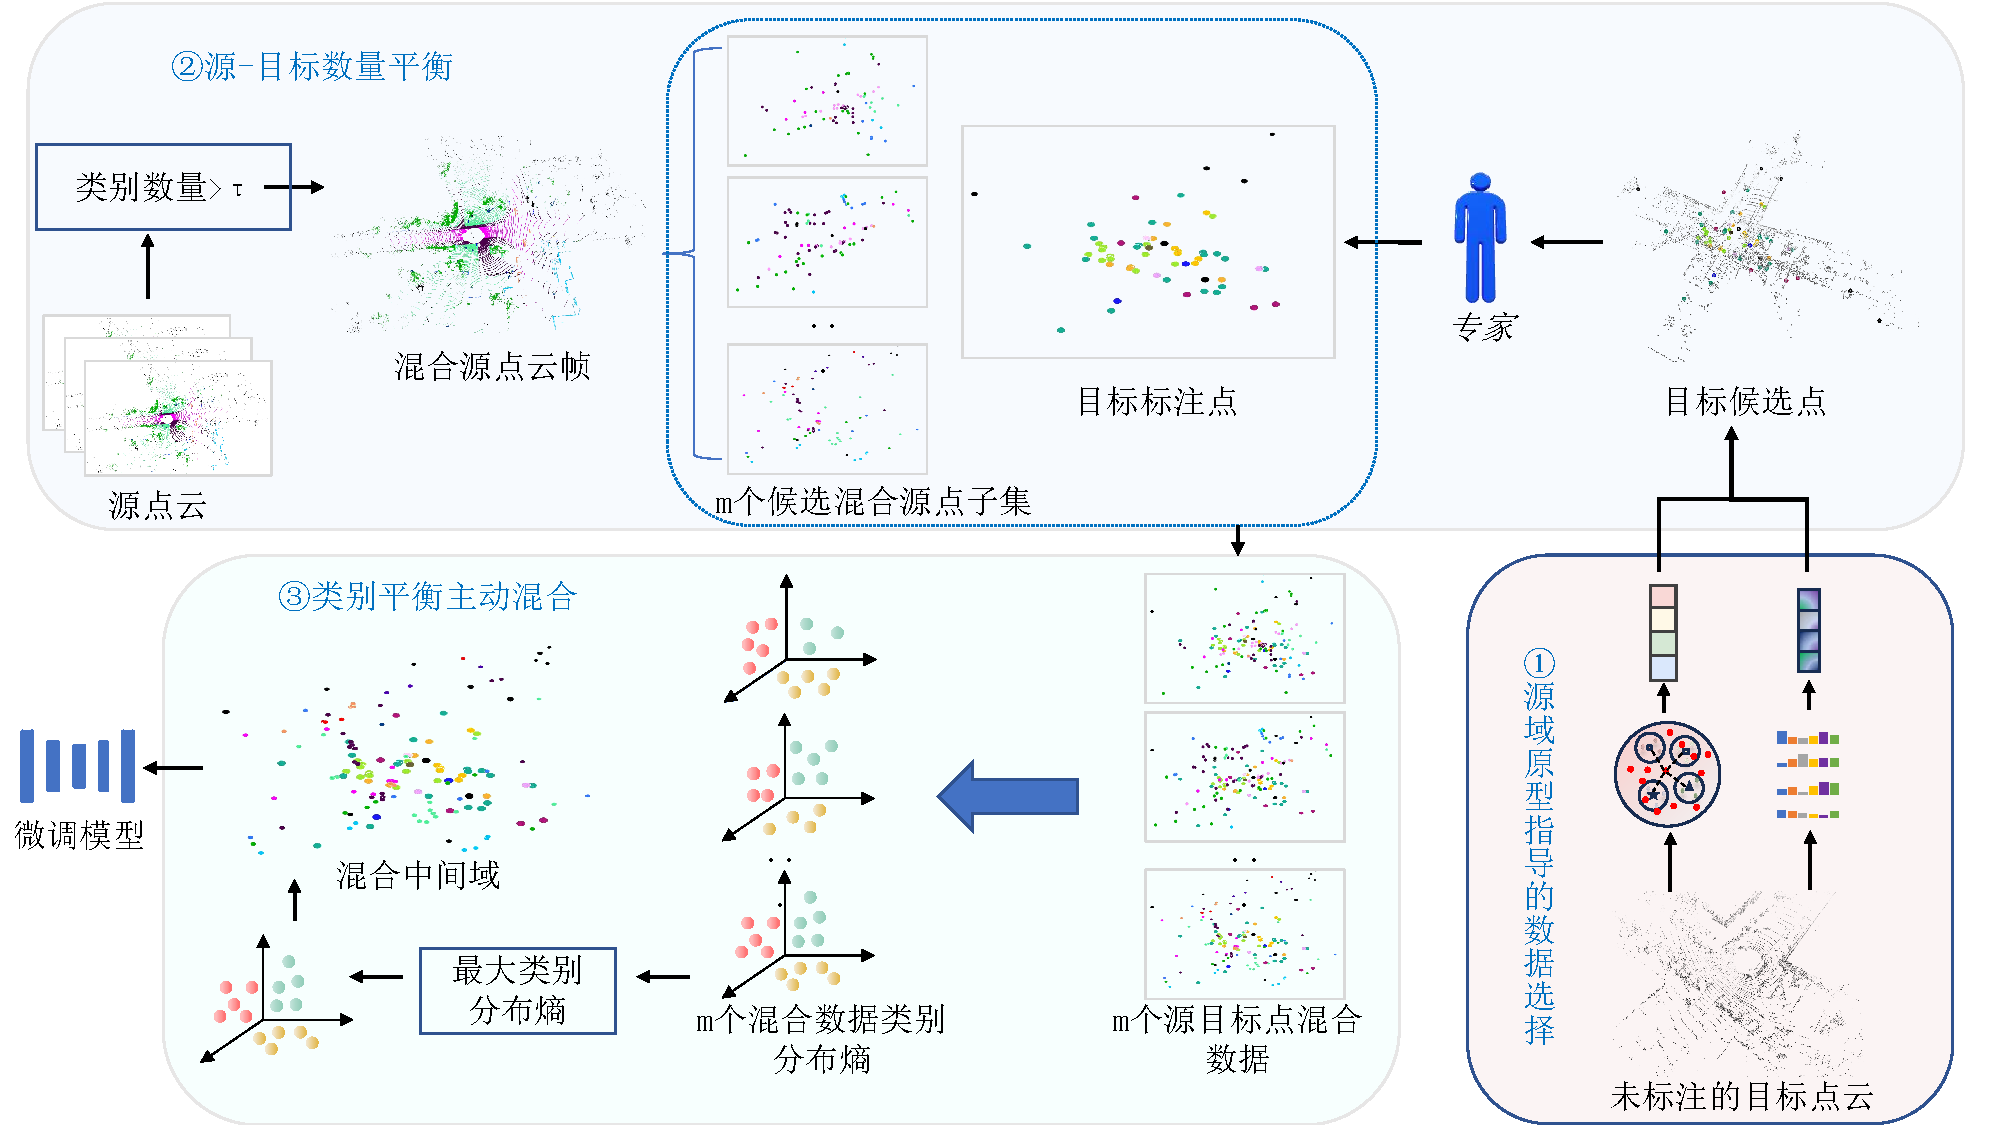
\includegraphics[width = \textwidth, scale=0.5]{ljx/figure/4-1framwork.pdf}
        \bicaption[\xiaosi 基于点云语义分割域适应的主动混合方法框架]{\wuhao 基于点云语义分割域适应的主动混合方法框架}{\wuhao Framework of active mixing for domain adaptation in point cloud semantic segmentation}
        \label{fig:4-1}
        \vspace{-0.3cm}
    \end{figure}
    % 为了探索mixing方法与主动学习在域适应任务上的深度结合,本章方法延续第三章的总体框架进行改进,改进后的框架如图 x-x 所示。算法基本流程主要由四个主要模块构成:\ding{172}源域原型构建模块,\ding{173}源原型引导的数据选择模块(SPAL),\ding{174}源-目标数量平衡模块以及\ding{175}类别平衡主动混合模块。在第三章中,我们设计了基于原型的主动学习方法,并初步探索结合Mixing方法构建出强壮的中间域数据,进一步缩减了域偏差,提升了模型的性能。然而对与mixing与主动学习的结合仍然有很大的探索空间。如何根据域偏差以及主动学习的特点来结合mixing仍然时一个可以探索的巨大问题。为了进一步形成两者间的高效促进作用从而获得更好的分割表现,本章方法在第三章的动态中间域模块进行了改进,分为了两个模块。一个是源-目标数量平衡模块:选择大于预设定类别数量的源域帧,并从中筛选与所匹配的目标域帧标注点数平衡的候选子集。另一个则是类别平衡主动混合模块:计算每个候选子集与目标域帧标注点混合后的类别分布熵值,选择值最大的候选模块构建类别相对平衡的中间域数据。
    
    % 我们初步探索结合了Mixing与主动学习并应用到语义分割域适应当中,并得到了可喜的效果

    % 应该是介绍一下总体的框架,然后说一些模块的组成,接着再说一下流程以及各模块在流程中的作用。
    \subsection{源-目标数量平衡算法}
    % 说一下问题及原因 - 引出我们的方法,接着对我们的方法的实现进行介绍(600个字左右就行)
    % 就是说明这个算法模块是怎么搞的
    前一章节的实验结果证明了主动学习与Mixing方法的结合取得了显著的效果。然而这只是对于两种方法结合的初步探索,对于他们的深度结合仍然有很大的探索空间。在主动域适应中,主动学习标注点的数量极少,又加之域间隙的存在,使得之前的连续场景、或者基于伪标签的Mixing方法与主动学习结合并不能发挥其最大的效果。如图\ref{fig:4-2}所示,本章的源-目标平衡算法旨在数量层面平衡混合的源域点和标注的目标点,对主动学习与Mixing的深入结合进行探索。
    
    在每一轮主动学习迭代中,将最新标注的目标点加入到已标注数据集中,更新数据集$\mathbf{T}^{al}_r$,更新公式如\eqref{eq:al_target_update}所示:
    \begin{equation}
        \label{eq:al_target_update}
        \mathbf{T}^{al}_r = \mathbf{T}^{al}_{r-1} \cup \mathbf{T}^{al}_r 
    \end{equation}
    式中,$\mathbf{T}^{al}_r$是当前主动学第$r$轮的主动标注最新数据集;而$\mathbf{T}^{al}_{r-1}$是上一轮即第$r-1$轮主动标注的数据集;其中$r$从1开始计算,并且当$r=0$时,$\mathbf{T}^{al}_0$为空集$\emptyset$。
    在主动学习阶段结束后,接着就是将已标注的最新的目标域数据与源数据混合。
    选择一帧带有标注的目标域数据,然后再随机匹配一帧源域数据,
    % 当然源域帧的筛选是有条件的,只有当帧中的类别的数量大于我们设定的阈值$\tau$时,这个源数据帧才有资格与当前的目标域帧进行混合,
    为了保证数据的质量,源域数据的筛选是有条件的,即仅当某一帧点云的类别数量大于预设的阈值$\tau$时,该帧数据才有资格与当前目标域数据进行混合,筛选过程如\eqref{eq:filter_source}所示,其中$\mathbf{S}_i = \{\mathbf{X}^S_i,\mathbf{Y}^S_i\}$,表示源域中的一帧点云数据。
    \begin{equation}
        \label{eq:filter_source}
        % \mathbf{S}_{mix} 
        \mathbf{M}_{mix}= \{\mathbf{S}_i | unique(\mathbf{Y}^S_i)> \tau\}, \quad \mathbf{Y}^S_i \in \mathbf{S}_i
    \end{equation}
    接着,从$\mathbf{M}_{mix}$中随机筛选一个源域帧$\mathbf{M}_i \in \mathbf{M}_{mix}$与目标域帧$\mathbf{p}_i$进行匹配,在匹配成功后,将从匹配的源域帧中,候选$m$个混合子集,这些候选子集中的点数与匹配的目标域中主动标注的点数量相同,候选点的公式如\eqref{eq:mix_subset}所示:
    % 首先,对于进行混合选择的源域数据进行过滤筛选,
    \begin{equation}
        \label{eq:mix_subset}
        \mathbf{Q} = \{\mathbf{q}_1,...,\mathbf{q}_m\}, 
        \quad
        \|\mathbf{q}_i\| = \|\mathbf{p}_i\|,
        \quad
        \mathbf{q}_i \subset \mathbf{Q},
        \quad
        \mathbf{p}_i \subset \mathbf{T}^{al}_r
    \end{equation}
    式中,$\mathbf{Q} \subset \mathbf{M}_i$为$m$个源域候选混合子集的集合;$\mathbf{q}_i$代表第$i$个候选子集;$\mathbf{p}_i$代表一个目标域点云帧中已标注点的集合;$\|\mathbf{q}_i\|$和$\|\mathbf{p}_i\|$分别代表候选子集$\mathbf{q}_i$和目标点云已标注点$\mathbf{p}_i$的数量。候选子集$\mathbf{Q}$将在下一个模块中进行筛选,以进一步缓解类别不平衡问题。

    % \vspace{-0.1cm}
    \begin{figure}[H]
        \vspace{-0.1cm}
        \centering
        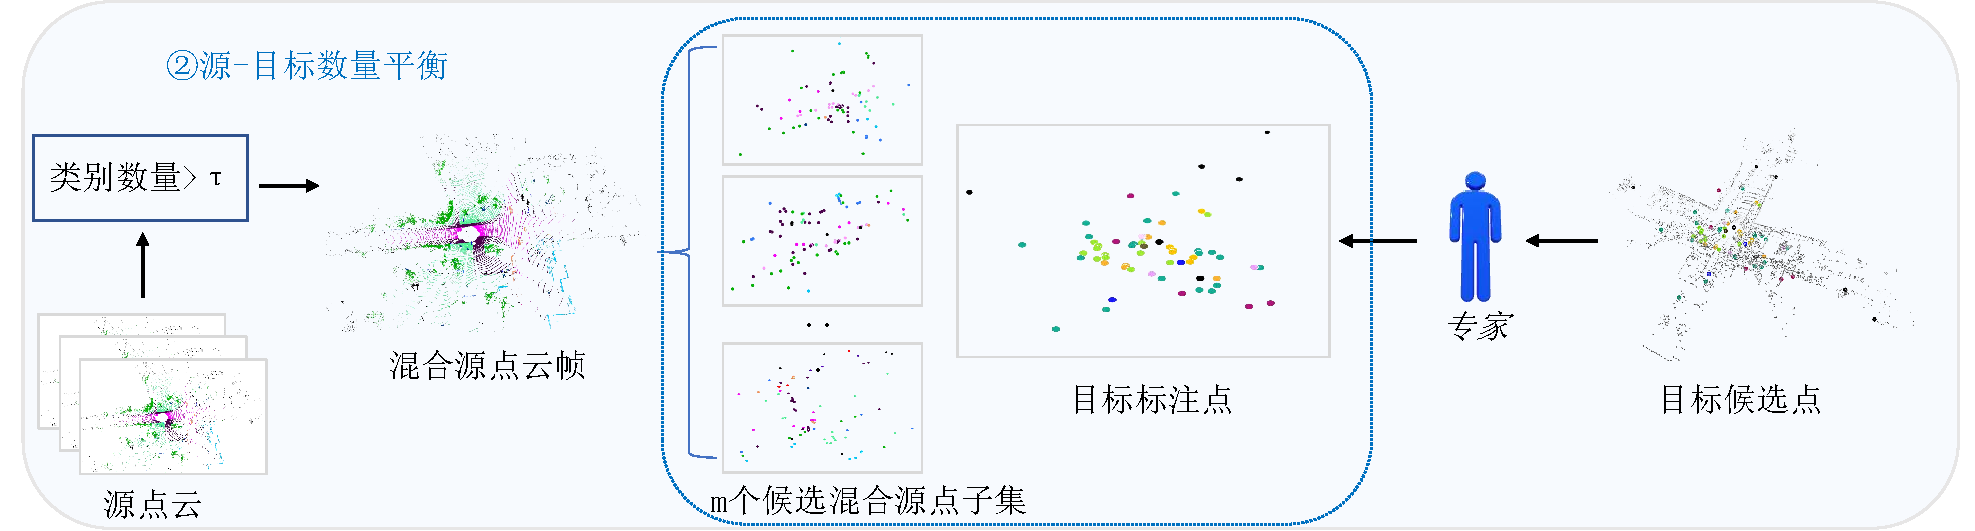
\includegraphics[width = \textwidth, scale=0.5]{ljx/figure/4-2s-t.pdf}
        \bicaption[\xiaosi 源-目标数量平衡模块]{\wuhao 源-目标数量平衡模块}{\wuhao Source-target amount balance module}
        \label{fig:4-2}
        \vspace{-0.4cm}
    \end{figure}
    % \vspace{-0.35cm}
    \subsection{类别平衡主动混合算法}  %使用select的进行写吧,看一下那篇文章
    % 同上,可以参考SELECT,但是一定要注意的是把体素换成是我们的点云帧才行(1000个字左右)
    % 主动学习普遍存在的一个问题是类别不平衡问题,所选择的点是无法提前预知的,所有的策略都是基于模型进行推测的,因此目标域中每一帧点云各类别所含点的数量差异显著。而标注后的类别分布的结果后验于主动学习选择的结果,为了解决这个问题,在域适应任务中源域中拥有大量且标注的语义类别点,本章的方法就是选择一些语义分布更加均衡的源域点进行混合,这样既可以学习到域不变特征,又可以缓解类别不平衡的问题。
    % 主动学习普遍存在类别不平衡的问题。由于所选取的点无法提前预知,所有策略均基于模型推测,标注后的类别分布结果又依赖于主动学习的选择,这会导致目标域中每一帧点云各类别所含标注点数存在显著差异。而在域适应任务中,源域通常拥有大量带标注的语义类别点。因此,为解决这一问题,本章方法通过选择可以使得混合后类别分布更平衡的源域点,并使之与目标域标注点进行混合形成中间域数据并用于模型微调,这不仅有助于学习域不变特征,也能有效缓解类别不平衡的问题。
    针对主动学习在目标域中引发的类别不平衡问题,本章提出了类别平衡主动混合算法。在主动学习中,由于所选取点的类别无法提前预知,因此主动选择的点往往会导致目标域每一帧点云中各类别之间所含标注点数存在显著差异。值得关注的是,在跨域点云分割任务中,源域通常具备大量完整标注且可直接利用的语义类别点。而这为本章解决主动学习选择的类别不平衡提供了一个思路。如图\ref{fig:4-3}所示,从源域数据上选择候选点并与目标域标注点混合,使得混合后的数据中类别分布相对平衡。混合后的中间域数据不仅有助于学习域不变特征,也能有效缓解类别不平衡的问题。%。因此,本章方法通过选择可以使得混合后类别分布更平衡的源域点,并使之与目标域标注点进行混合形成中间域数据并用于模型微调,这不仅
    % 基于从源-目标数量平衡模块所得到的$m$个候选子集,本小节的平衡模块旨在从$\mathbf{Q}$中选取一个候选子集$\mathbf{q}_i$,使得其在所有被选中的候选子集中的类别分布最均衡。为此将根据混合后的点云集真实标签分布计算的熵作为选择的指标,以减轻标签不平衡。具体而言,训练集都是混合后的中间域数据,记$N_{all}$代表训练集中所有已标注的点数,$N_c$则为其中属于类别c的点的总数。而$N_{mix}$,$i$则代表候选子集$\mathbf{q}_i$与匹配的目标域标注点的的总点数,$N_{mix}^c$表示其中真实标签为类别c的点数。为确定是否应选择候选子集$\mathbf{q}_i$来实现更平衡的类别分布,通过将已选择的标注点总数$N_{all}$与当前选子集$\mathbf{q}_i$与匹配的目标域混合后的总点数相加,计算类别c的相对比例$\{R_{i,c}\}^C_{c=1}$,公式如\eqref{eq:class_rate}所示:
    \begin{figure}[H]
        % \vspace{0.3cm}
        \centering
        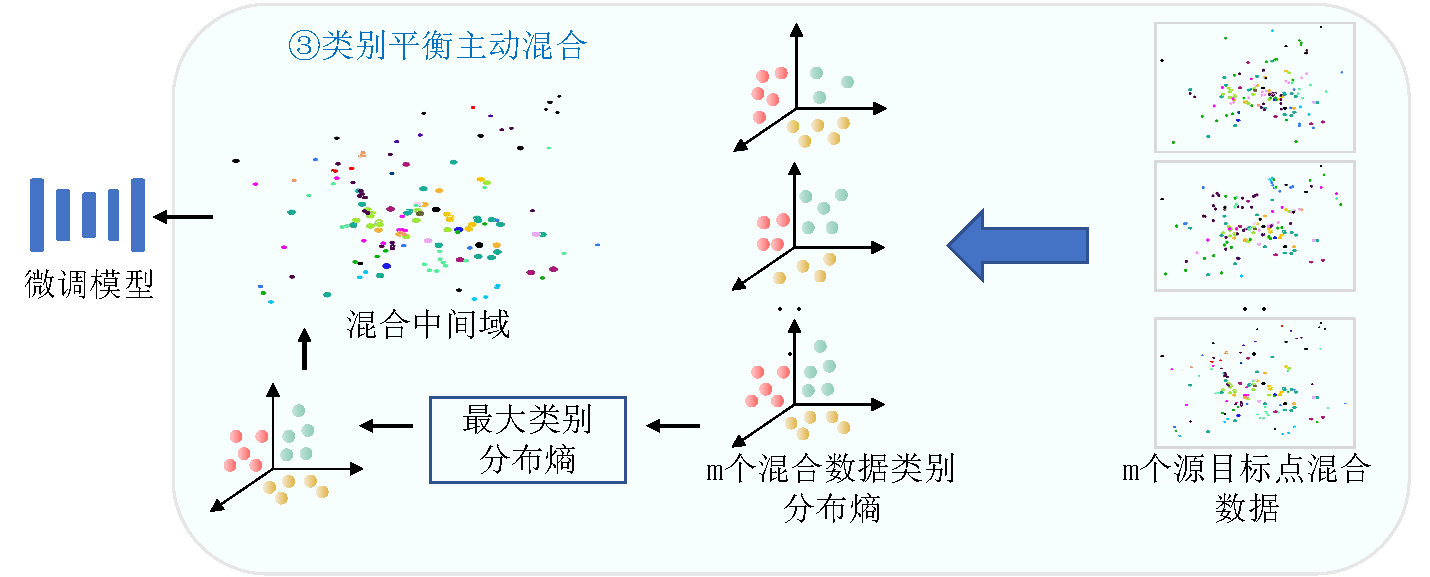
\includegraphics[width = \textwidth, scale=0.5]{ljx/figure/4-3am-b.pdf}
        \bicaption[\xiaosi 类别平衡主动混合模块]{\wuhao 类别平衡主动混合模块}{\wuhao Class-balanced active mixing module}
        \label{fig:4-3}
        \vspace{-0.6cm}
    \end{figure}
    基于源-目标数量平衡模块生成的$m$候选子集,平衡模块的核心任务是从集合$\mathbf{Q}$中选取最优子集$\mathbf{q}_{max}$,使得该子集与已选数据组合后的整体类别分布达到最优
    % \vspace{-0.1cm}
    % 在后续内容加文字才行
    % \vspace{-0.35cm}
    平衡状态。为实现这一目标,本模块采用信息熵作为量化指标,即通过计算候选子集与目标域数据混合后的真实标签分布熵值,筛选出能够最大程度缓解类别不平衡的候选子集。具体实施过程定义如下:设定已经构建的动态中间域训练数据集包含$N_{all}$个已标注点,其中类别$c$的标注点数量为$N_c$。对于混合源域帧中的候选子集$\mathbf{q}_i$,将其与对应目标域标注数据进行混合,混合后形成的数据子集包含$N_{mix}$个点,其中类别$c$的标注点数量为$N_{mix}^c$。为评估候选子集$\mathbf{q}_i$的平衡效果,需计算其引入后各类别的相对分布比例。具体方法是将已标注数据总量$N_{all}$与候选混合数据量$N_{mix}$进行叠加,按公式\eqref{eq:class_rate}逐类计算混合后的分布比例$\{R_{i,c}\}^C_{c=1}$。%最终通过后续的分布熵值比较实现最优子集选择。
    \begin{equation}
        \label{eq:class_rate}
        R_{i,c} = \frac{N_c+N^c_{mix}}{N_{all}+N_{mix}}
    \end{equation}
    % 发大发发打发打发发大发水电费阿斯蒂芬撒地方撒旦防守打法阿斯蒂芬啊范德萨发第三方萨达防守打法士大夫萨达防守打法士大夫水
    % 该方法通过动态叠加候选子集与目标域数据,基于信息熵最大化优化混合后的类别分布比例,系统性缓解整体类别不平衡问题。
    % 该方法考虑了整体类别平衡,即将选择后的混合数据与整体已混合的数据进行相加并得到最终的类别分布比例,这样可以保证整体的类别平衡
    % 该方法考虑了整体类别平衡,即通过将选择后的混合数据与已混合的整体数据相加,从而得到最终的类别分布比例,确保在整个数据集中保持类别的平衡性。
    同时,为了保证在同一个量纲下比较,对$R_{i,c}$使用softmax函数进行归一化处理,得到$\hat{R}_{i,c}$,如公式\eqref{eq:class_softmax}所示:
    \begin{equation}
        \label{eq:class_softmax}
        \hat{R}_{i,c}=\frac{e^{R_{i,c}}}{\sum^C_{c=1}e^{R_{i,c}}}
    \end{equation}
    其表示选择候选子集$\mathbf{q}_i$与当前已标注的目标点云帧混合后,各类别所占点数的归一化概率。再然后,通过计算类别分布的熵值来可作为候选子集的选择评判指标,如公式\eqref{eq:class_entropy}所示:
    \begin{equation}
        \label{eq:class_entropy}
        H_i(\hat{R}_{i})=-\sum_{c=1}^{C} \hat{R}_{i,c}\log(\hat{R}_{i,c})
    \end{equation}
    式中,$H_i$表示选择候选子集$\mathbf{q}_i$混合后类别分布的熵值结果,并选择熵值最大的一个候选子集$\mathbf{q}_{max}=\{\mathbf{X}_{\mathbf{q}_{max}},\mathbf{Y}_{\mathbf{q}_{max}}\}$作为最终混合的源域集,与目标域标注点集$\mathbf{p}_i=\{\mathbf{X}_{p_i},\mathbf{Y}_{p_i}\}$组成新的中间域数据集$\mathbf{I}=\{\mathbf{\hat{X},\hat{Y}}\}$,如公式\eqref{eq:mix_final}所示:
    \begin{equation}
        \label{eq:mix_final}
        \begin{aligned}
            \mathbf{\hat{X}}=concat\{\mathbf{X}_{\mathbf{q}_{max}},\mathbf{X}_{\mathbf{p}_i}\}
            \\
        \mathbf{\hat{Y}}=concat\{\mathbf{Y}_{\mathbf{q}_{max}},\mathbf{Y}_{\mathbf{p}_i}\}
        \end{aligned}
    \end{equation}
    式中,$\mathbf{\hat{X}}$表示混合的点数据;$\mathbf{\hat{Y}}$则表示对应的标签。%将最终选择出的后选子集与目标域点进行混合,同时
    最后更新训练集总点数以及类别点数,公式如\eqref{eq:update_numeber}所示:
    \begin{equation}
        \label{eq:update_numeber}
        \begin{aligned}
            N_c=N_c+N^c_{mix}, \quad
            N_{all}=N_{all}+N_{mix}
        \end{aligned}
    \end{equation}
    
    \subsection{损失函数}
    % 对于后续的模型训练仅使用混合后的中间域数据进行微调训练,而混合后的数据都是含有标注的,因此本章使用交叉熵损失函数做为我们的优化损失函数,
    在后续的训练中,模型仅采用混合后的中间域数据进行微调优化。由于这些数据均包含标注信息,因此所有实验均采用交叉熵损失函数作为优化策略,如公式\eqref{eq:cross_entropy}所示,其中$\hat{x}_{i} \in \hat{\mathbf{X}}$;$\hat{y}_{i} \in \hat{\mathbf{Y}}$。
    \begin{equation}
        \label{eq:cross_entropy}
        \mathbf{L}_{\text{CE}} = - \frac{1}{|I|} \sum_{i \in I} \sum_{c=1}^{C} \hat{y}_{i}^{c} \log h(\hat{x}_{i}^{c})
    \end{equation}

    \section{实验评估}
    \subsection{实验设置}
    在本章实验中,同样使用MinkowskiNet\upcite{MinkowskiNet}在Annotator中的PyTorch实现版本作为目标分割网络模型,并使用随机梯度下降(SGD)\upcite{SGD}作为学习优化器。所有实验都在单张NVIDIA RTX A6000 GPU上进行训练。本章方法同样在真实到真实以及合成到真实的跨域场景下分别进行了实验。对于所有的场景,主动学习全程总共执行5次迭代并达到预设标注预算。由于在四个跨域数据集上的映射类别数量不同,参数$\tau$在SynLiDAR$\to$SemanticKITTI、SynLiDAR$\to$SemanticPOSS、SemanticKITTI$\to$nuScenes和nuScenes$\to$SemanticKITTI分别设置为13、9、6、6,候选参数$m$统一设为10。此外,对于其他实验参数的配置仍延续第三章的实验设定。
    \subsection{实验结果}
    本章方法同样在合成到真实场景下的跨域数据集SynLiDAR$\to$SemanticKITTI和SynLiDAR$\to$SemanticPOSS,以及真实到真实场景下的跨域数据集SemanticKITTI
    $\to$nuScenes和nuScenes$\to$SemanticKITTI上做了相应的实验,并与最先进的方法以及前一章的方法进行了对比以验证其有效性。为了公平比较,如果没有特殊标明标注预算的情况下,默认都是在0.1\%标注预算下做出的实验结果。
    \subsubsection{合成到真实场景}
    \begin{table}[H]
	\renewcommand{\arraystretch}{1}
    \centering
    \setlength{\tabcolsep}{10mm}
    \bicaption[\xiaosi 第三章方法与其他域适应方法在SynLiDAR\(\to\)SemanticKITTI数据上的比较]{\wuhao 本方法与其他域适应方法在SynLiDAR\(\to\)SemanticKITTI数据上的比较}{\wuhao Comparison with other domain adaptation methods on SynLiDAR\(\to\)SemanticKITTI}
    \label{tab:4-1}
    \wuhao
    \begin{tabular}{lccc}
        \toprule[1.5pt]
        \textbf{方法} & \textbf{域适应} & \textbf{标注} & \textbf{结果} \\
        \midrule
        Source-Only   & -          & -       & 22.8 \\
        Target-Only   & -          & 100\%       & 60.1 \\
        AADA          & UDA & -       & 23.0 \\
        AdvEnt        & UDA & -       & 25.8 \\
        CRST          & UDA & -       & 26.5 \\
        ST-PCt        & UDA & -       & 28.9 \\
        PolarMix      & UDA & -       & 32.2 \\
        CoSMix        & UDA & -       & 31.0 \\
        DGT-ST        & UDA & -       & 43.1 \\
        MME           & SSDA & 0.04\%  & 24.5 \\
        APE           & SSDA & 0.04\%  & 25.1 \\
        APE-PCT       & SSDA & 0.04\%  & 27.0 \\
        CoSMix-SSDA   & SSDA & 0.04\%  & 34.3 \\
        本章方法       & SSDA   & 0.04\%   & 50.5 \\
        Annotator     & ADA   & 0.1\%     & 57.7 \\
        前章方法     & ADA   & 0.1\%     & 58.7 \\
        \textbf{本章方法}       & ADA   & 0.1\%     & \textbf{65.5} \\
        \bottomrule[1.5pt]
    \end{tabular}
\end{table}
    \vspace{-0.2cm}
    本章在SynLiDAR$\to$SemanticKITTI跨域数据集上的实验如表\ref{tab:4-1}所示,分析对比不同的结果可知,在没有任何域适应的情况下,预训练(Source-Only)模型在目标域上的性能非常低,仅有22.8\%,这说明直接将源域训练的模型用到目标域效果很差。而全监督模型(Target-Only)达到了60.1\%的结果,这说明域间隙的存在会导致在源域训练好的模型在目标域上性能急剧下降。
    % 说明目标域本身的标注数据确实能极大提升效果,但现实中很难获取这么多标注数据。因此需要研究如何在标注有限的情况下提升性能。

    在不需要目标域标注的无监督域适应(UDA)方法中,DGT-ST的效果最好,达到43.1\%,比Source-Only提升了近20个百分点,但相比Target-Only仍有较大差距。这说明即使不标注目标域数据,通过域适应也能部分缩小域间差异,但还不能完全解决问题。
    为了与半监督域适应(SSDA)方法进行公平比较,将标注预算降低到与半监督同一量级即0.04\%,即使在这种极少量的标注下,本章方法仍达到了50.5\%的结果,比同样标注量的CoSMix-SSDA高出了近16个百分点。这说明在标注极少的情况下,本章方法能更有效地利用有限的标注信息。

    在与主动域适应(ADA)方法进行比较时,标注比例提升到0.1\%,本章方法的结果达到了65.5\%,不仅比前章方法提高了近7个百分点,甚至超越了Target-Only,这说明本章方法构建的中间域增强了模型的性能,学习到了源和目标域的信息,缓解了类不平衡,因此超越了全监督结果。当然,超越Target-Only本方法并非先例,在之前的相关域适应文章中\upcite{schachtsiek2023classf}也有做到。另外,值得注意的是,虽然标注量增加了2.5倍,但性能提升幅度远高于标注量的增长比例,这说明在前一章的基础上,结合本章主动混合方法,充分发挥了它们的最佳性能。
    % 能够充分发挥二者的深度结合优势。
    % 本章主动混合方法结合前一章源域指导的主动学习方法,能够充分发挥了其最佳性能。
    
    % \begin{table}[htbp]
\begin{table}[H]
	\renewcommand{\arraystretch}{1}
    \centering
    \setlength{\tabcolsep}{10mm}
    \bicaption[\xiaosi 第四章方法与其他域适应方法在SynLiDAR\(\to\)SemanticPOSS数据上的比较]{\wuhao 本章方法与其他域适应方法在SynLiDAR\(\to\)SemanticPOSS数据上的比较}{\wuhao Comparison with other domain adaptation methods on SynLiDAR\(\to\)SemanticPOSS}
    \label{tab:4-2}
    \wuhao
    \begin{tabular}{cccc}
        \toprule[1.5pt]
        \textbf{方法} & \textbf{域适应} & \textbf{标注} & \textbf{结果} \\
        \midrule
        Source-Only   & -           & -       & 34.6 \\
        Target-Only   & -           & 100\%       & 58.0 \\
        CRST\upcite{zou2019confidence}          & UDA & -       & 27.1 \\
        ST-PCT\upcite{xiao2022transfer}        & UDA & -       & 29.6 \\
        PolarMix\upcite{xiao2022polarmix}      & UDA & -       & 30.4 \\
        CoSMix\upcite{saltori2022cosmix}        & UDA & -       & 40.4 \\
        DGT-ST\upcite{yuan2024density}        & UDA & -       & 50.8 \\
        MME\upcite{saito2019semi}           & SSDA & 0.01\%  & 33.2 \\
        APE\upcite{APE}           & SSDA & 0.01\%  & 30.3 \\
        APE-PCT\upcite{xiao2022transfer}       & SSDA & 0.01\%  & 31.2 \\
        CoSMix-SSDA\upcite{saltori2023compositional}   & SSDA & 0.01\%  & 41.0 \\
        本章方法       & SSDA   & 0.01\%   & 57.5 \\
        Annotator\upcite{Annotator}     & ADA   & 0.1\%     & 52.0 \\
        前章方法       & SSDA   & 0.1\%   & 56.6 \\
        \textbf{本章方法}       & ADA   & 0.1\%     & \textbf{60.2} \\
        \bottomrule[1.5pt]
    \end{tabular}
\end{table}
    如表\ref{tab:4-2}结果显示,在SynLiDAR$\to$SemanticPOSS数据集上域差异依然显著。在无监督域适应(UDA)中,DGT-ST以50.8\%的表现达到最优,但距离全标注仍有7个百分点的差距。本章方法在0.01\%的极低标注预算下达到了57.5\%的结果,远超CoSMix-SSDA,接近Target-Only水平。当与主动域适应方法(ADA)进行比较时,标注量提升至0.1\%,本章方法以60.2\%的结果分别超越前章方法和Annotator 3.6和7.8个百分点,超过全监督(Targe-Only)2.2个百分点,这证明本章的主动混合方法是有效果的,在结合第三章的方法后可以大幅度提升模型性能。
    % 最后,提供了合成到真实场景下的可视化结果,以真实标签为参照,与前章方法进行对比,以证明本章方法的有效性,可视化结果如图\ref{fig:4-5}所示:
    % \vspace{-0.1cm}
    % \begin{figure}[h]
    %     \centering
    %     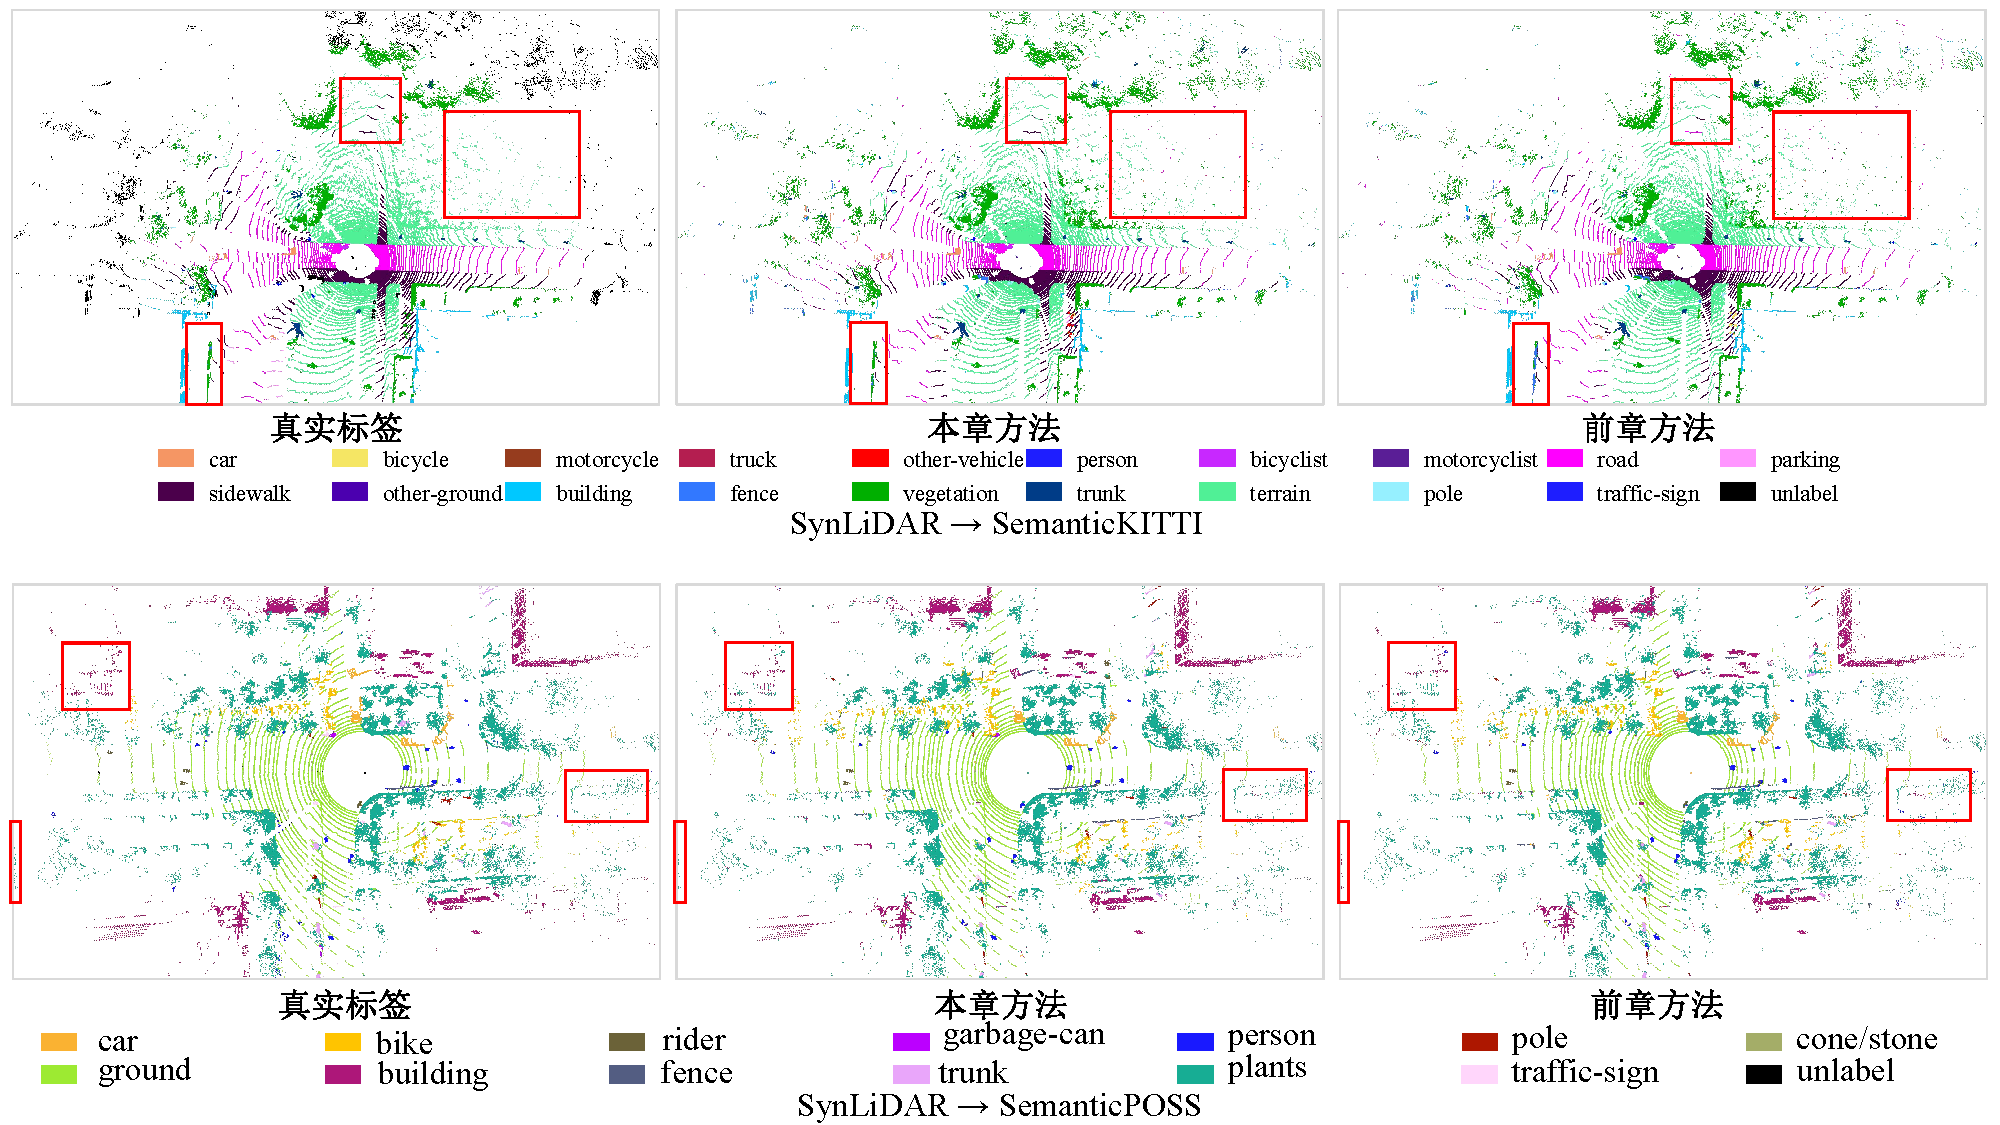
\includegraphics[width = \textwidth, scale=0.5]{ljx/figure/4-5s2r.pdf}
    %     \bicaption[\xiaosi 类别平衡主动混合模块]{\wuhao 类别平衡主动混合模块}{\wuhao Class-balanced active mixing module}
    %     \label{fig:4-5}
    % \end{figure}
    % \vspace{-0.35cm}
    % 证明第三章所提出的主动学习筛选能大幅降低标注成本选择对域适应最有帮助的域差异点,同时也证明本章的主动混合方法可以大幅提升其效果。
    % 通过表4-2的数据对比,可以看出不同域适应方法在SynLiDAR→SemanticPOSS数据集上的表现差异。从Source-Only(34.6)和Target-Only(58.0)的对比来看,两个领域的差异依然显著,直接迁移源域模型的效果有限,而完全标注目标域虽能大幅提升性能,但实际应用中标注成本过高的问题依然存在。  
    % 在无监督域适应(UDA)方法中,DGT-ST的表现最好,达到了50.8,远高于其他UDA方法(如CRST的27.1、CoSMix的40.4)。这说明DGT-ST在无标注情况下能较好地缓解域差异,但距离Target-Only仍有7分左右的差距,表明无监督方法在复杂场景中仍有优化空间。  
    % 当标注量仅为0.01\%(SSDA场景)时,本章方法以57.5的得分远超其他SSDA方法。例如,CoSMix-SSDA仅达到41.0,而本章方法比其高出16.5分,甚至接近Target-Only的58.0。这表明即使标注量极少,通过动态筛选源域数据并与目标域混合的策略,能更有效地利用有限标注信息,显著缩小域间差距。值得注意的是,本章方法的SSDA结果(57.5)甚至超过了部分标注量更高的ADA方法(如Annotator的52.0),进一步验证了该策略的高效性。  
    % 当标注量提升到0.1\%(ADA场景)时,本章方法得分60.2,不仅比前章方法(56.6)提高了3.6分,还超过了Annotator的52.0。虽然标注量增加了10倍(从0.01\%到0.1\%),但性能提升幅度(从57.5到60.2)相对较小,可能说明在极低标注量下模型性能已接近上限,或需要更精细的样本选择策略。此外,本章方法在ADA场景下的结果(60.2)与Target-Only(58.0)的差距缩小到仅2.2分,这表明通过主动学习筛选高价值样本,能在少量标注下实现接近全标注的效果,大幅降低实际应用成本。  

    % 整体来看,本章方法在两种标注场景下均展现出较强优势,尤其是在极低标注量(0.01\%)时,其性能已接近部分高标注量方法的结果,验证了动态混合方法在跨域数据平衡中的重要性。
    \subsubsection{真实到真实场景}
    SemanticKITTI$\to$nuScenes的结果如表\ref{tab:4-3}所示,Source-Only模型在目标域的结果仅为33.7\%,而全标注的Target-Only模型则达到了82.7\%,这验证了真实到真实跨域场景中源域与目标域的巨大差异。在无监督域适应(UDA)方法中,LiDOG以34.9\%的表现最优,但仍远低于全标注结果,表明纯无监督策略在复杂域差异下的局限性。在主动域适应(ADA)场景下,本章方法以81.0\%的结果显著超越Annotator的75.9\%,提升幅度达5.1分,且与全监督(Target-Only)的差距缩小至1.7个百分点,同时与前章方法相比,提升了4.5个百分点。从上述实验结果可知本章方法通过主动混合方法有效利用有限标注信息与源域数据,在极低标注成本下逼近全标注性能,证明了其在真实跨域场景中的有效性。
    % \begin{table}[htbp]
\begin{table}[H]
	\renewcommand{\arraystretch}{1}
    \centering
    \setlength{\tabcolsep}{12mm}
    \bicaption[\xiaosi 第四章方法与其他域适应方法在SemanticKITTI\(\to\)nuScenes数据上的比较]{\wuhao 本章方法与其他域适应方法在SemanticKITTI\(\to\)nuScenes数据上的比较}{\wuhao Comparison with other domain adaptation methods on SemanticKITTI\(\to\)nuScenes}
    \label{tab:4-3}
    \wuhao
    \begin{tabular}{cccc}
        \toprule[1.5pt]
        \textbf{方法} & \textbf{域适应} & \textbf{标注} & \textbf{mIoU(\%)} \\
        \midrule
        Source-Only   & -       & -           & 33.7 \\
        Target-Only   & -       & 100\%           & 82.7 \\
        Mix3D\upcite{nekrasov2021mix3d}         & UDA     & -   & 31.5 \\
        CoSMix\upcite{saltori2022cosmix}        & UDA     & -   & 29.8 \\
        SN\upcite{wang2020train}              & UDA   & -     & 25.8 \\
        RayCast\upcite{langer2020domain}        & UDA    & -    & 30.9 \\
        LiDOG\upcite{saltori2023walking}        & UDA      & -       & 34.9 \\
        前章方法       & ADA    & 0.1\%      & 76.5 \\
        Annotator\upcite{Annotator}     & ADA     & 0.1\%     & 75.9 \\
        \textbf{本章方法}       & ADA    & 0.1\%      & \textbf{81.0} \\
        \bottomrule[1.5pt]
    \end{tabular}
\end{table}
    如表\ref{tab:4-4}数据显示,在nuScenes$\to$SemanticKITTI的实验结果中,Source-Only模型仅得32.5\%,而Target-Only模型通过全标注数据达到85.4\%,再次印证域差异的显著影响。在无监督域适应(UDA)方法中,LiDOG以41.2\%的表现依然取得最优,但仍与全标注结果相差44.2个百分点。在标注量仅0.1\%的主动域适应(ADA)场景下,本章方法以86.2\%的结果超越目标域全监督(Target-Only)0.8个百分点,远超Annotator的81.8\%,超越前章方法3.2个百分点。本章方法的突破性结果表明,通过主动混合方法在极低标注量下超越了全标注的性能,进一步证明了本章方法的真实有效性。
    % 大幅降低了实际应用中对标注数据的依赖。这一结果进一步验证了源-目标协同优化策略在跨域任务中的高效性。
    % \begin{table}[htbp]
\begin{table}[H]
	\renewcommand{\arraystretch}{1}
    \centering
    \setlength{\tabcolsep}{12mm}
    \bicaption[\xiaosi 第四章方法与其他域适应方法在nuScenes\(\to\)SemanticKITTI数据上的比较]{\wuhao 本章方法与其他域适应方法在nuScenes\(\to\)SemanticKITTI数据上的比较}{\wuhao Comparison with other domain adaptation methods on nuScenes\(\to\)SemanticKITTI}
    \label{tab:4-4}
    \wuhao
    \begin{tabular}{cccc}
        \toprule[1.5pt]
        \textbf{方法} & \textbf{域适应} & \textbf{标注} & \textbf{mIoU(\%)} \\
        \midrule
        Source-Only   & -       & -           & 32.5 \\
        Target-Only   & -       & 100\%           & 85.4 \\
        Mix3D\upcite{nekrasov2021mix3d}         & UDA    & -   & 32.4 \\
        CoSMix\upcite{saltori2022cosmix}        & UDA     & -   & 36.8 \\
        SN\upcite{wang2020train}              & UDA   & -     & 23.6 \\
        RayCast\upcite{langer2020domain}        & UDA    & -    & 31.5 \\
        LiDOG\upcite{saltori2023walking}        & UDA      & -       & 41.2 \\
        前章方法       & ADA    & 0.1\%      & 83.0 \\
        Annotator\upcite{Annotator}     & ADA     & 0.1\%     & 81.8 \\
        \textbf{本章方法}       & ADA    & 0.1\%      & \textbf{86.2} \\
        \bottomrule[1.5pt]
    \end{tabular}
\end{table}
    \subsubsection{分割可视化结果}
    \vspace{-0.1cm}
    \begin{figure}[h]
        \centering
        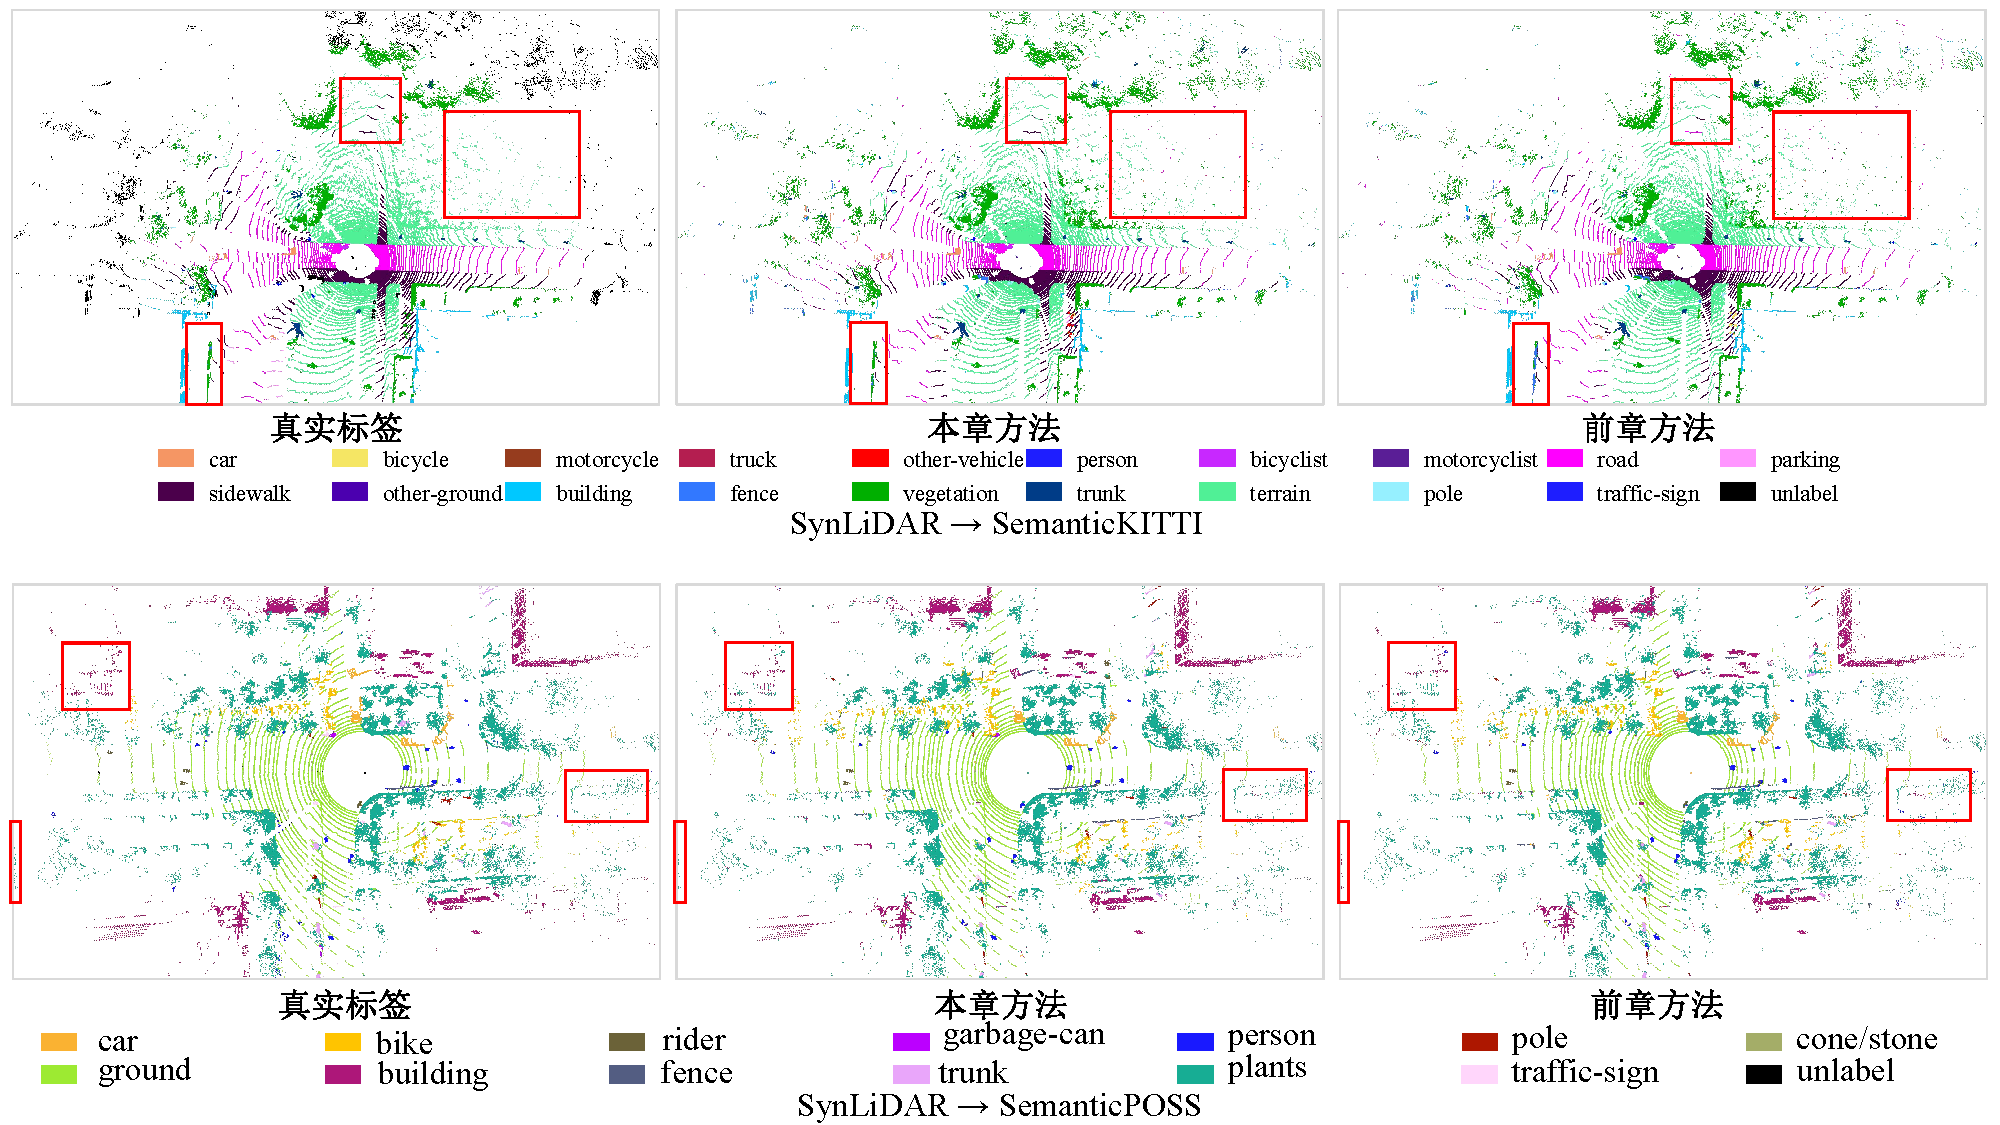
\includegraphics[width = \textwidth, scale=0.5]{ljx/figure/4-5s2r.pdf}
        \bicaption[\xiaosi 第四章方法在合成到真实场景分割可视化图]{\wuhao 本章方法在合成到真实场景分割可视化图}{\wuhao Visualization of the segmentation results in the synthetic-to-real}
        \label{fig:4-5}
    \end{figure}
    \vspace{-0.35cm}
    为了进一步证明本章方法的有效性,提供了合成到真实场景下的可视化结果如图\ref{fig:4-5}所示。以真实标签为参照,与前章方法进行对比,使用红框标出差异区域,可以看到本章方法在一些语义边界处有着更好的辨别效果。同样的,本章也提供了真实到真实场景下的可视化结果如图\ref{fig:4-6}所示。本章方法在人造物品、人行道等边缘类别相比前章均取得了更好的分割效果。
    \vspace{-0.1cm}
    \begin{figure}[h]
        \centering
        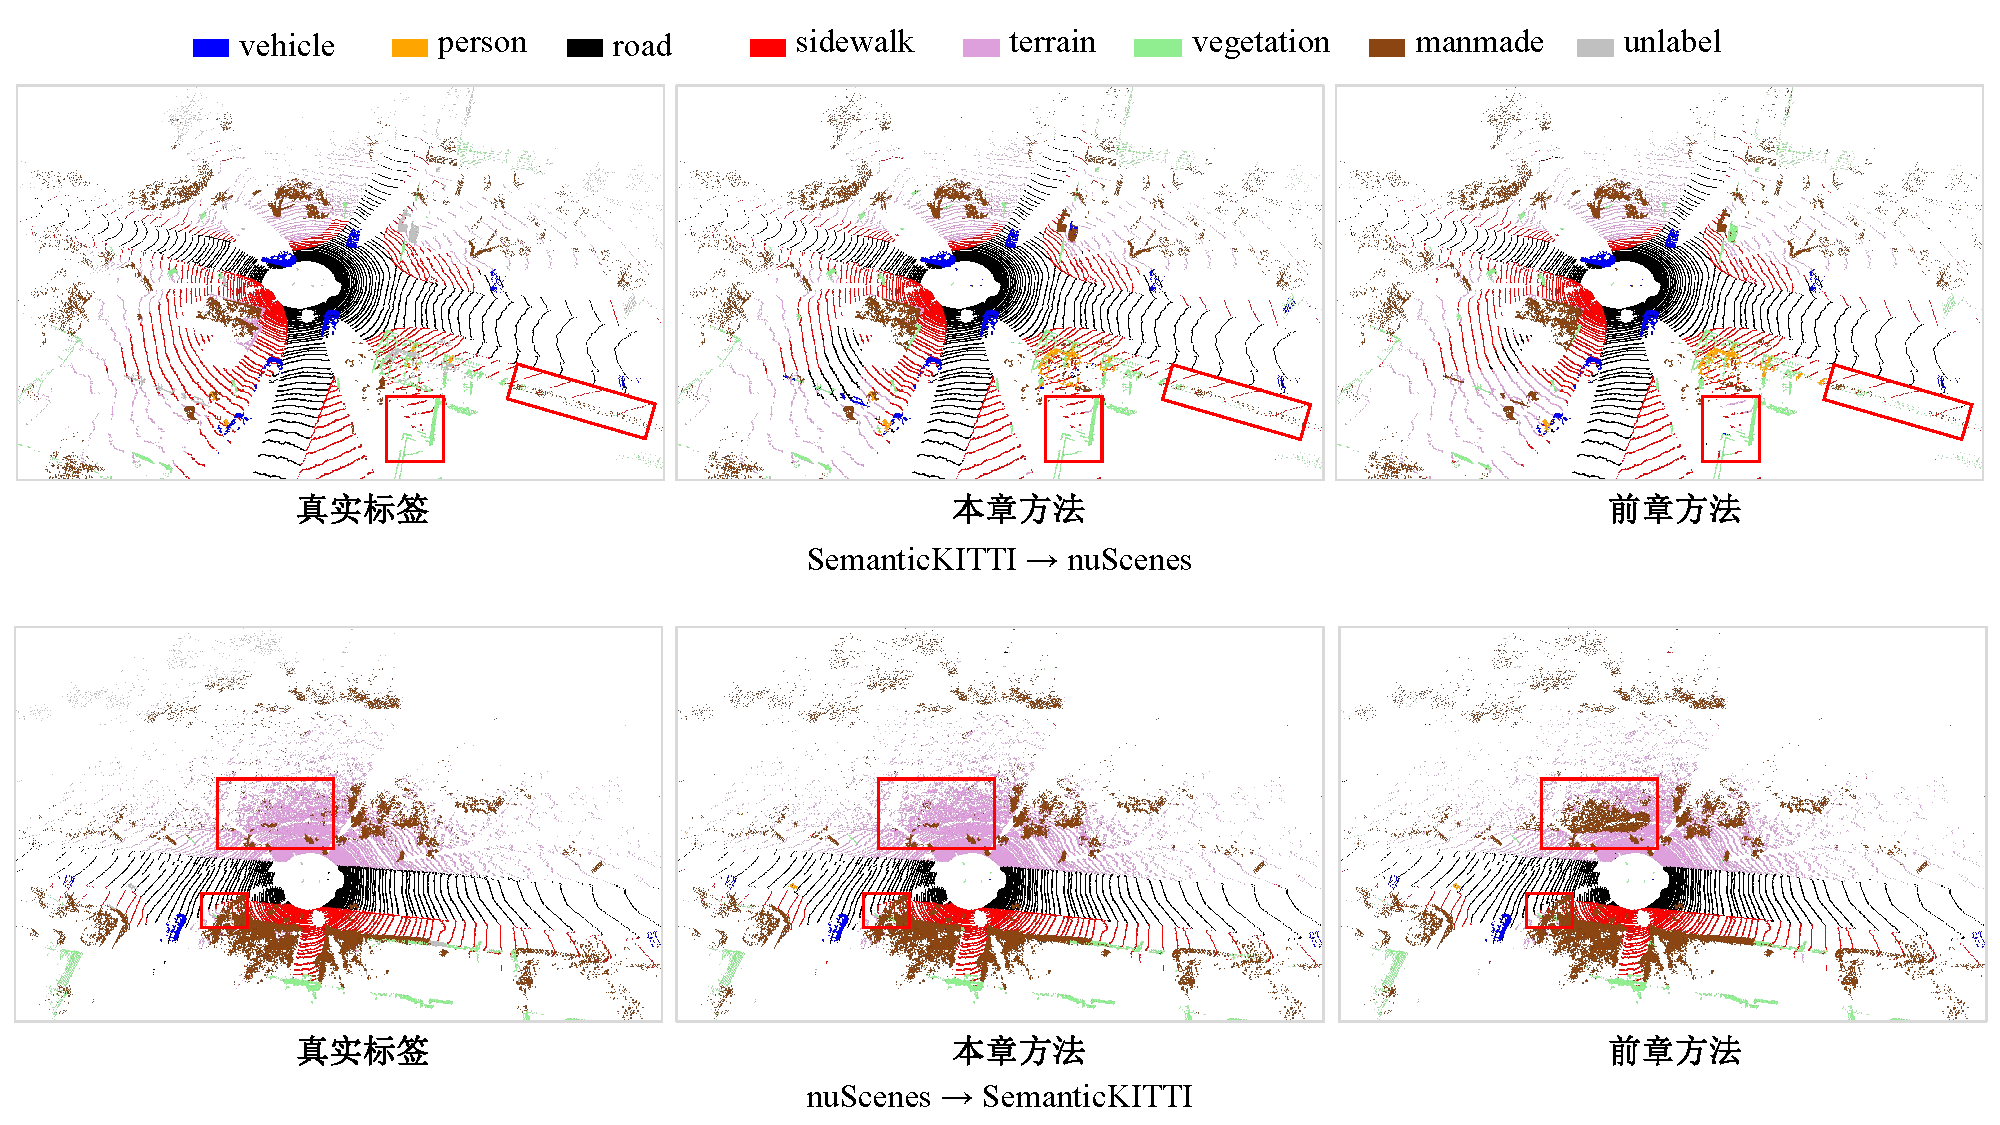
\includegraphics[width = \textwidth, scale=0.5]{ljx/figure/4-6r2r.pdf}
        \bicaption[\xiaosi 第四章方法在真实到真实场景分割可视化图]{\wuhao 本章方法在真实到真实场景分割可视化图}{\wuhao Visualization of the segmentation results in the real-to-real}
        \label{fig:4-6}
    \end{figure}
    \vspace{-0.35cm}
    \subsection{消融对比实验}
    % 把所有的能放的图和表全放上来
    \subsubsection{对比实验}
    \begin{table}[H]
	\renewcommand{\arraystretch}{1}
    \centering
    \setlength{\tabcolsep}{10mm}
    \bicaption[\xiaosi 第四章方法与其他Mixing方法在SynLiDAR$\to$SemanticKITTI数据上的比较]{\wuhao 本章方法与其他Mixing方法在SynLiDAR$\to$SemanticKITTI数据上的比较}{\wuhao Comparison with other mixing methods on SynLiDAR$\to$SemanticKITTI}
    \label{tab:4-6}
    \wuhao
    \begin{tabular}{cccc}
        \toprule[1.5pt]
        \textbf{主动学习} & \textbf{Mixing方法} & \textbf{标注} & \textbf{结果} \\
        \midrule
        \multirow{3}{*}{SPAL} & LaserMix\upcite{kong2023lasermix} & 0.1\% & 39.6 \\
        ~& PolarMix\upcite{xiao2022polarmix} & 0.1\% & 46.6 \\
        ~& \textbf{Ours} & 0.1\% & \textbf{65.5} \\
        \bottomrule[1.5pt]
    \end{tabular}
\end{table}
    为证明本章方法的有效性,在SynLiDAR$\to$SemanticKITTI上进行了与其他传统Mixing方法的对比实验,在SPAL框架下统一采用0.1\%标注量进行公平比较,实验结果如表\ref{tab:4-6}所示。实验中,PolarMix和LaerMix都是按照1/4比例进行混合,即源和目标交换自身1/4圆周角度内的点或者1/4线束角度内的点进行混合。在相同标注条件下,LaserMix和PolarMix方法分别取得39.6\%和46.6\%的性能结果,而本章提出的方法以65.5\%的显著优势超越了它们,性能提升幅度达25.9\%和18.9\%。这一结果验证了传统混合方法在跨域数据融合时对类别分布不敏感,数量过多导致模型学习的知识更偏向源域等问题,而本章方法通过双域数量平衡算法以及熵驱动的源域筛选动态平衡算法,能够精准选择与目标域互补的源域样本,有效缓解混合过程中的类别不均衡问题。%因此,基于固定几何变换的混合方法通常难以适应复杂域差异场景,本章方法在相同标注约束下的突破性表现,进一步证明了基于点云语义分割域适应的主动混合方法在跨域主动学习中价值。
    \vspace{-0.1cm}
    \begin{figure}[H]
        \centering
        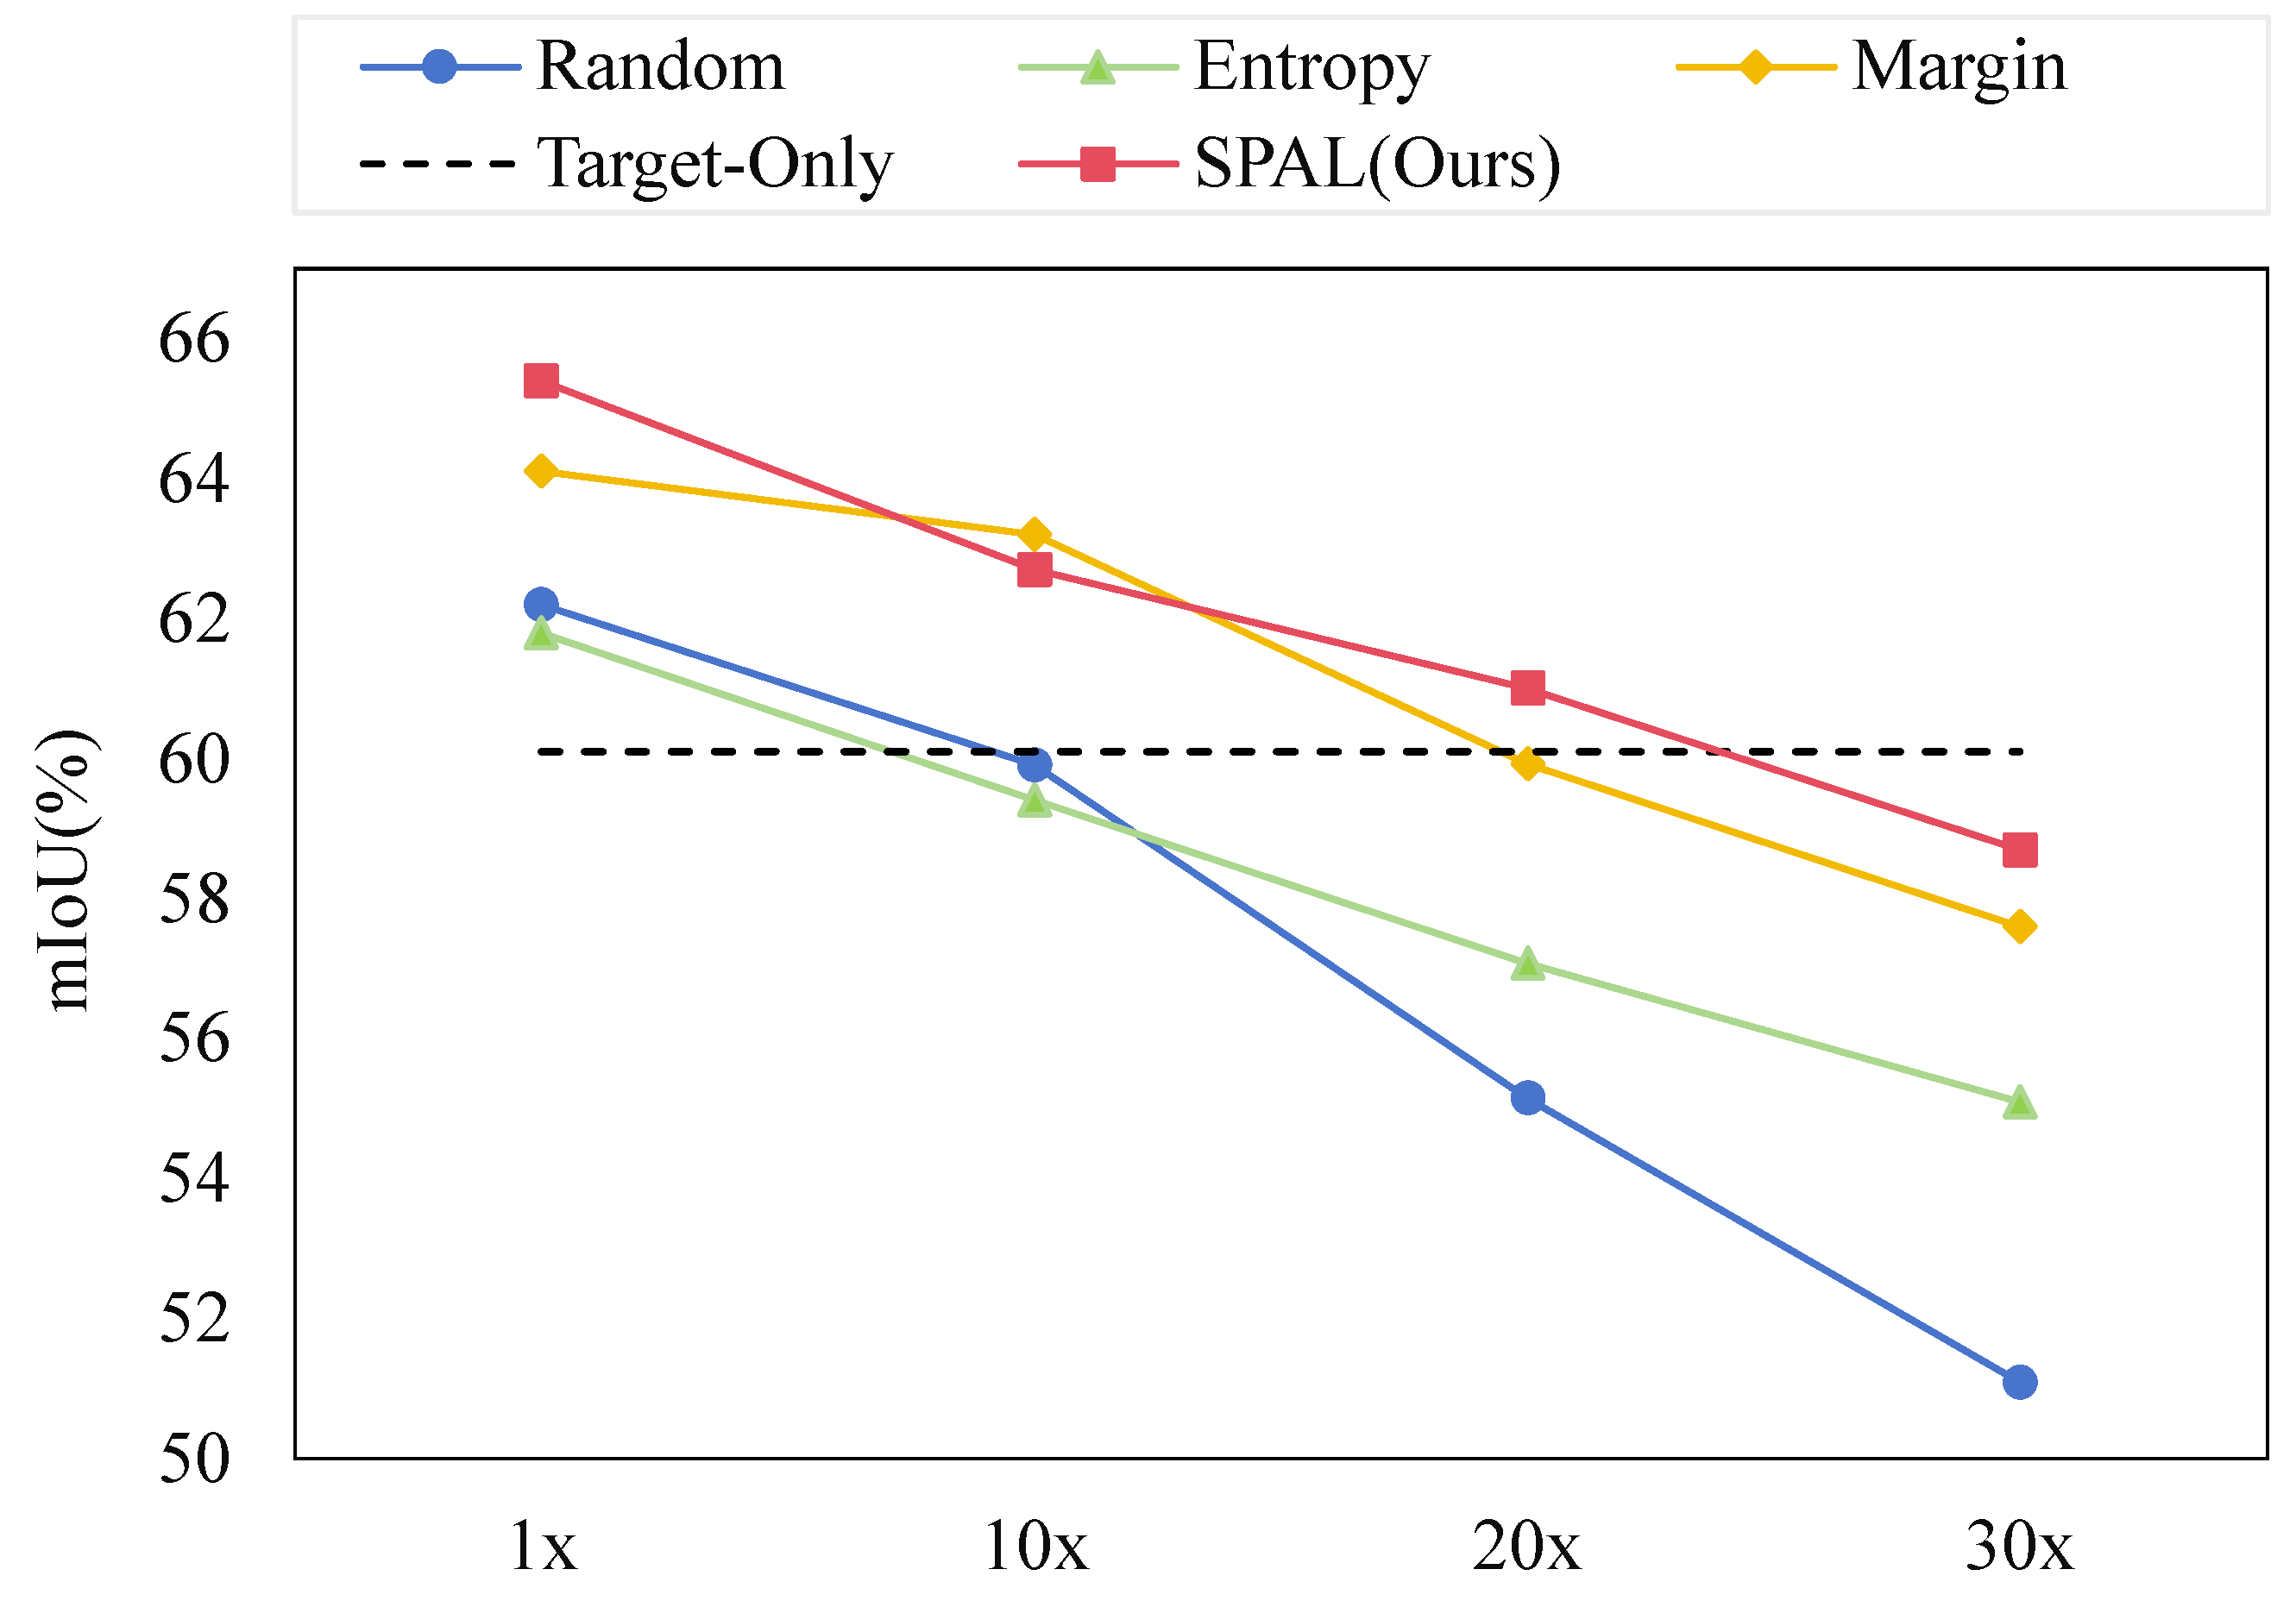
\includegraphics[width = \textwidth]{ljx/figure/4-compare-al-mixing.pdf}
        \bicaption[\xiaosi 第四章方法结合不同主动学习在多个混合比例下的对比结果]{\wuhao 本章方法结合不同主动学习在多个混合比例下的对比结果}{\wuhao Comparison results of different active learning methods under various mixing ratios}
        \label{fig:4-compare-al-mixing}
    \end{figure}
    \vspace{-0.35cm}
    如图\ref{fig:4-compare-al-mixing}所示,本章在SynLiDAR$\to$SemanticKITTI数据集上进行了对比实验,展示了不同主动学习策略在不同源-目标混合比例下的性能对比。其中,1x代表的是本章提出的源-目标域数量平衡算法(即源域与目标域数据按1:1比例动态混合),10x代表源域与目标域数据按10:1比例动态混合,20x和30x则分别代表源域与目标域数据按20:1和30:1比例进行动态混合。实验结果显示,在默认0.1\%的标注预算下,本章源-目标数量平衡方法在多种主动学习方法中均取得了最优的结果,证明了该方法的有效性,根据域适应以及主动学习的特点,简单高效的提升了性能。而在源-目标域数量平衡算法下,与前一章提出的SPAL方法的结合又是最高的,达到了65.5\%的结果,这证明了SPAL与本章方法结合的有效性。
    
    为了进一步证明本章方法结合前章SPAL方法的的有效性,在四个跨域数据集(SynLiDAR$\to$SemanticKITTI、
    SynLiDAR$\to$SemanticPOSS、SemanticKITTI$\to$nuScenes、nuSc-
    enes$\to$SemanticKITTI)上均进行了实验。如表\ref{tab:4-5}所示,在四个跨域数据实验中,结合两章的算法均取得最高结果,且稳定超越其他主动学习方法。这验证了第四章提出的主动混合方法与第三章SPAL框架结合的有效性和普适性。这一跨数据集的全面优势表明,源-目标平衡机制能够适配不同域差异场景,显著提升模型的性能。
    % \vspace{-0.1cm}
    % 换成竖的
% \begin{table}[ht]%[t]
%     \centering
%     \resizebox{\linewidth}{!}
%     {
%         \large
%         \begin{tabular}{@{}l|c|c@{}}
%             \toprule
%             Methods & SynLiDAR $\to$ SemanticKITTI & SynLiDAR $\to$ SemanticPOSS \\
%             \midrule
%             Source-/Target-Only & 22.0 / 61.1 & 34.5 / 57.9 \\
%             % \midrule
%             Random & 62.2 & 58.3 \\
%             Entropy & 61.8 & 55.6 \\
%             Margin & 64.0 & 60.0 \\
%             \revision{VCD}~\cite{xie2023annotator} & 56.8 & 45.5 \\
%             \textbf{SPAL (Ours)} & \revision{\textbf{65.5}} & \textbf{60.2} \\
%             \bottomrule 
%         \end{tabular}
%     }
%     \caption{Comparison of different active query strategies for domain adaptation on MinkNet~\cite{choy20194d} with a 0.1\% budget and a mixing rate of $1$x. Our query strategy consistently achieves superior performance both SynLiDAR $\to$ SemanticKITTI and SynLiDAR $\to$ SemanticPOSS.}
%     \label{tab:active_query}
% \end{table}

% \begin{table}[htbp]
\begin{table}[H]
    \vspace{-0.05cm}
	\renewcommand{\arraystretch}{1}
    \centering
    \setlength{\tabcolsep}{10mm}
    \bicaption[\xiaosi 第四章方法结合不同主动学习方法结果对比]{\wuhao 本章方法结合不同主动学习方法结果对比}{\wuhao  Comparison with different active learning methods that incorporate this chapter's modules}
    \label{tab:4-5}
    \wuhao
    \begin{tabular}{cccc}
        \toprule[1.5pt]
        \textbf{数据集} & \textbf{方法} & \textbf{标注} & \textbf{mIoU(\%)} \\
        \midrule
        \multirow{4}{*}{SynLiDAR\(\to\)SemanticKITTI} & 
        Random              & 0.1\%        & 62.2 \\
        ~ & Entropy\upcite{Entropy}             & 0.1\%        & 61.8 \\
        ~ & Margin\upcite{Margin}              & 0.1\%        & 64.0 \\
        ~ & \textbf{SPAL}          & 0.1\%        & \textbf{65.5} \\
        \multirow{4}{*}{SynLiDAR\(\to\)SemanticPOSS} & 
        Random              & 0.1\%        & 58.3 \\
        ~ & Entropy\upcite{Entropy}             & 0.1\%        & 55.6 \\
        ~ & Margin\upcite{Margin}              & 0.1\%        & 60.0 \\
        ~ & \textbf{SPAL}          & 0.1\%        & \textbf{60.2} \\
        \multirow{4}{*}{SemanticKITTI\(\to\)nuScenes} & 
        Random              & 0.1\%        & 85.7 \\
        ~ & Entropy\upcite{Entropy}             & 0.1\%        & 83.2 \\
        ~ & Margin\upcite{Margin}              & 0.1\%        & 85.9 \\
        ~ & \textbf{SPAL}          & 0.1\%        & \textbf{86.2} \\
        \multirow{4}{*}{nuScenes\(\to\)SemanticKITTI} & 
        Random              & 0.1\%        & 77.7 \\
        ~ & Entropy\upcite{Entropy}             & 0.1\%        & 76.5 \\
        ~ & Margin\upcite{Margin}              & 0.1\%        & 80.7 \\
        ~ & \textbf{SPAL}          & 0.1\%        & \textbf{81.0} \\
        \bottomrule[1.5pt]
    \end{tabular}
    \vspace{-0.1cm}
\end{table}
    % \vspace{-0.2cm}
    \subsubsection{消融实验}
    最后,在SynLiDAR$\to$SemanticKITTI跨域数据上进行了本章的消融实验,主动学习默认使用0.1\%的标注预算。如表\ref{tab:4-7}所示,结果证明本章提出的两个模块对性能提升均有贡献。当任何模块都不用时,基线结果仅为22.84\%。当仅使用第三章的SPAL模块时,性能提升至58.70\%。在引入源-目标平衡模块(STNB)后,性能跃升至65.46\%,表明在域差异场景下,数量平衡的混合能帮助模型学习到更有效的域不变特征,显著缓解域差异问题,最终完整方法以65.51\%达到最优,类别平衡主动混合模块(CBAM)进一步优化了0.05个百分点,表明其在解决类别平衡问题上有所贡献。
    % 说明其在解决类别平衡问题以及性能提升上也有所贡献。
    \begin{table}[H]
	\renewcommand{\arraystretch}{1}
    \centering
    \setlength{\tabcolsep}{8mm}
    \bicaption[\xiaosi 第四章方法消融实验]{\wuhao 本章方法模块消融实验}{\wuhao Ablation experiments on modules}
    \label{tab:4-7}
    \wuhao
    \begin{tabular}{cccc}
        \toprule[1.5pt]
        \textbf{SPAL} & \textbf{STNB} & \textbf{CBAM} & \textbf{mIoU(\%)} \\
        \midrule
          & & & 22.84 \\
          \checkmark  & & & 53.50 \\
          \checkmark  & \checkmark & & 65.46 \\
          \checkmark  & \checkmark & \checkmark & \textbf{65.51} \\
        \bottomrule[1.5pt]
    \end{tabular}
\end{table}
    \section{本章小结}
    本章提出了一种面向点云语义分割域适应任务的主动混合方法,重点探索主动学习与Mixing方法协同作用对域适应性能的提升。通过设计源-目标数量平衡算法(STNB),在每轮主动学习中动态匹配源域与目标域标注点的数量,确保混合数据中双域信息均衡融合。
    % 同时,类别平衡主动混合算法(CBAM)利用类别分布的熵值,计算多个候选源域子集与目标域标注集混合后,分布最为均衡的集合,增强主动学习与混合方法的协同效率。
    同时,类别平衡主动混合算法(CBAM)通过计算混合后类别分布的熵值,评估多个候选源域子集与目标域标注集混合后的分布平衡性,从而选择最为均衡的集合。这种方法增强了主动学习与混合策略的协同效率。
    最后,在两个跨域场景下的四个跨域数据集上的实验表明,在0.1\%标注量下,本章完整方法在四个跨域数据集中均达最优的性能,并且显著超越了传统混合方法,最后的消融实验显示模块协同作用时性能提升最大,充分验证了本章算法的有效性。


% 第5章
\chapter{总结与展望}
\thispagestyle{others}
\pagestyle{others}
\xiaosi

\section{主要结论}
% 背景->问题->引出本文
% 其实没有具体的要求,就是写一下点云语义分割的应用,然后再写一下问题,主要是把问题描述的具体一点。
% 然后再写针对上述的问题,本章做了什么研究
% 点云语义分割是三维场景感知的关键一环,也是实现自动驾驶、机器人、增强现实等领域高级智能的一项重要技术。然而,由于目前优秀的深度学习模型都是基于逐点标注的数据训练而来的,但是对点云进行逐点标注却非常的困难,这阻碍了这些优秀算法的落地。因此,如何在无标注或者少量标注下得到一个性能优秀的模型变得非常重要。域适应方法通过将一个全标注源域训练得到的模型迁移到未标注的目标域上去,从而实现对新目标数据的学习同时降低标注。主动学习则是通过对选择一些最具价值的点进行标注而后对模型进行训练。而主动域适应则时结合了主动学习和域适应方法,得到更有效的方案。尽管现在的方法已经在二维图像语义分割领域取得了一定的成果,但是对于三维点云的研究却缺乏探索:
% 首先,目前的一些主动域适应的方法都是在二维图像领域的,对于三维点云语义分割域适应却缺乏研究,而三维数据与二维数据有所区别,且数量级也不同,因此一些适用于图像的主动域适应无法直接应用到点云上。
% 其次,传统的主动学习方法多是用于单域数据的,并未考虑两域间的域偏移问题,因此如果直接应用到域适应场景下,可能会导致选择次优点,从而无法发挥其最佳作用。
% 第三,未充分利用标注后的目标数据和全标注的源域数据,发挥其最大价值。由于域偏差的存在,且主动学习标注的目标点远少于源域点, 因此在适应的过程中可能导致域偏移的积累,导致模型偏向源数据,从而导致模型学习到次优的效果。
% 针对上述分析的问题,通过大量阅读相关文献并进行了实验验证,本文的主要研究内容归结如下:
点云语义分割是实现三维场景感知的关键技术,也是自动驾驶、机器人和增强现实等领域实现高级智能的重要基础。然而,目前多数优秀深度学习模型均依赖于逐点标注数据进行训练,而点云逐点标注工作极为繁琐且耗时,这成为制约这些模型实际应用的主要障碍。因此,在无标注或仅有少量标注数据的条件下获得高性能模型,显得尤为重要。
% 域适应方法通过将在全标注源域上训练得到的模型迁移到未标注目标域,从而实现对新数据的学习并降低标注成本。
域适应方法旨在将基于全标注源域训练得到的模型迁移至未标注的目标域,以实现对新数据的学习并降低标注成本。
主动学习则通过选择最具价值的样本进行标注以优化模型训练效果,而主动域适应则融合了二者的优势,提供了一种更为有效的解决方案。尽管该方法在二维图像语义分割领域已取得一定成果,但针对三维点云的研究仍显不足,主要存在以下问题:
第一,目前多数主动域适应方法集中于二维图像领域,因三维点云数据在结构和数量级上均存在显著差异,直接移植图像方法往往难以奏效。
第二,传统主动学习方法通常针对单一数据域设计,未能充分考虑源域与目标域之间的域偏移问题,因此在域适应场景下直接应用可能导致样本选择次优,影响最终效果。
第三,现有方法未能充分整合标注后的目标数据与全标注的源域数据,因主动学习选取的目标点数量远低于源域数据量,容易在迁移过程中积累域偏移,使模型倾向于源域,从而难以获得最优性能。基于上述问题,通过大量文献阅读和实验验证,本文的主要研究内容可归纳如下:

% 1)通过大量阅读相关文献,总结并分析了目前相关领域的研究现状和进展,对所研究领域有一个系统的了解。包括点云语义分割方法,主动学习方法域自适应方法以及分割中的Mixing方法。通过上述大量文献的阅读,并根据个人理解和观点对现有方法进行归类总结,分析总结了现有方法的优点和不足,同时,对这些问题想出诸多有意义的研究思路和解决方案。
% 1)通过大量阅读相关文献,对点云语义分割方法、主动学习、域自适应以及分割中的混合方法等相关领域的研究现状和进展进行了系统总结和分析。基于个人的理解与观点,对现有方法进行了归类,总结了各自的优势与不足,并提出了一些具有实际意义的研究思路和解决方案。

% 2)对点云语义分割、主动学习和域自适应相关的基础背景知识做了详细总结。包括点云的常见表示方式,点云语义分割任务的概念、常见模型以及评估指标,主动学习的基本概念和流程以及域自适应任务的概念、目标以及常见的域对齐方式等。并对跨域点云语义分割相关任务中常用公开的数据集进行了介绍整理。

1)提出了一种基于点云语义分割域适应的主动学习方法。该方法通过构建出的源域原型,指导目标数据的选择,同时结合不确定性,筛选出兼具高不确定性和域差异性的目标点,用以高效提升模型的性能。随后将这些选择后的目标点进行标注,同时结合Mixing方法,构建兼具双域信息的中间域数据,帮助模型学习到更加鲁棒的域不变特征,进一步缩小域间隙。%文中首先详细的介绍了该方法的研究动机和贡献,接着详细的阐述了该方法中的三个模块,包括源域原型构建模块、原型指导的数据选择模块、动态中间域构建模块。最后在合成到真实以及真实到真实的4个跨域数据集上,对提出的方法进行大量实验和可视化分析证明了该方法的有效性。

2)提出了一个基于点云语义分割域适应的主动混合方法。该方法在第三章方法框架基础上,深入探索了域适应场景下主动学习与Mixing方法的结合,并将动态中间域构建模块更改为了两个模块:源-目标数量平衡模块和类别平衡动态混合模块。该方法改善了模型迁移过程中因源域数据过多而导致的模型学到的知识偏向源域的问题,同时减缓了主动学习类别不平衡问题。
最后,在合成到真实以及真实到真实的四个跨域数据集上,对所提方法进行了大量实验和可视化分析,充分验证了其有效性。
% 最后同样在合成到真实以及真实到真实的4个跨域数据集上,对该方法进行了大量实验和可视化分析以证明了其有效性。

\section{研究展望}
本文的研究中,对于所提出的两个方法分别解决了不同的问题。基于点云语义分割域适应的主动学习方法中,提出了一种适用于点云语义分割域适应的主动学习方法,
% 弥补了三维点云领域的研究空缺,
在结合Mixing后发挥最大优势,超越传统主动学习方法。基于点云语义分割域适应的主动混合方法,则是在上个方法的框架下,对点云语义分割域适应场景下主动学习与Mixing的结合进行了深入研究和探索,通过构建数量及类别平衡的中间域数据缓解了迁移过程中的域偏移累积问题和类别不平稳问题。虽然上述研究在与同领域方法的比较中取得了先进的表现,但是受限于时间、设施等多种因素,仍然存在很大的局限和提升空间。同时,基于对目前前沿技术的理解以及所做的大量实验验证分析,归结了一些点云语义分割域自适应领域中仍存在的需要进一步解决或者缓解的问题。为此,本文对未来研究做出了如下展望:

% 1)目前本研究的实验的跨域场景虽然涵盖了合成到真实以及真实到真实两个场景,但是这些场景都是基于室外数据进行的,还未对室内场景下跨域任务进行尝试,而室外和室内数据之间密度和场景大小均有差异,因此本文方法不能保证在室内跨域场景下也同样表现良好,因此提升模型的泛化能力,使其在室内外跨域数据集上能表现良好是未来需要探索的一个重要方向。
1)模型泛化能力提升。目前,本研究的跨域实验虽然涵盖了合成到真实和真实到真实两个场景,但均基于室外数据集进行的测试,尚未在室内场景下验证。由于室外与室内数据在密度和场景规模上存在显著差异,本文方法在室内跨域任务中的适用性尚无保障。因此,未来研究需着力提升模型的泛化能力,以确保其在室内外跨域数据集上均能获得良好表现,这将是一个重要的探索方向。

% 2)进一步利用未标注数据方面,虽然本文通过主动学习方法已经筛选出数量较少但价值极高的目标点,但剩余约98\%以上的目标点仍未得到利用。未来工作应探索将主动学习与伪标签技术相结合的方法,以充分挖掘大量未标注数据的潜力,提升数据利用率,并进一步增强模型的泛化性能和分割效果。这将为降低标注成本和实现高效跨域点云语义分割提供新的研究思路和技术支持。
2)进一步挖掘未标注数据的潜在价值。尽管本研究通过主动学习策略筛选出极少的高价值目标域样本进行标注,但占总量99\%的未标注点云数据仍未被有效利用。为解决这一资源浪费问题,未来研究可探索主动学习与伪标签技术的协同优化框架:首先通过构建基于不确定性和域间差异的双重评估机制,对未标注点云进行可信度分层,筛选出置信度高于阈值的点生成伪标签;同时设计对抗噪声干扰的自适应校正模块,利用点云局部几何一致性特征对伪标签进行拓扑纠偏。此外,可建立动态迭代优化机制,在每轮主动学习标注新增样本后,同步更新伪标签生成模型,形成标注数据增强与伪标签质量提升的正向循环。但也需要特别关注伪标签噪声传播与域偏移累积的耦合效应。同时,通过在特征空间构建源域标注数据、目标域标注数据、目标域伪标签数据的三体平衡约束,从而在扩大训练数据规模的同时维持模型的域不变特征表达能力。

% 3)语义选择的主动混合,虽然本文提出了一个类别平衡的主动混合策略,但是基于域适应下的混合探索还远远不够。混合可以进行有选择的混合,目前只是对源域的数据进行了约束,但是目标域上的数据仍然可以通过选择混合到其他目标帧上去,可以通过语义的平衡分别从源域和目标域上选择数据而后混合。
3)语义选择的主动混合。尽管本文提出了一种基于类别平衡的主动混合方法,但在域适应条件下,对混合方法的探索仍远远不够。目前的策略仅对源域数据进行了约束,而目标域数据仍有较大改进空间。未来可以在混合过程中采用更具选择性的策略,分别从源域和目标域中依据语义平衡挑选数据,然后进行有针对性的混合,从而更充分地利用目标域信息,进一步提升模型在跨域任务中的性能。

% 4)大模型融合,当今最火的当属大模型,其具有优秀的文本理解和逻辑推理能力,目前很多领域和方法都开始引入并结合大模型,从而进一步提升结果表现,因此,而对于域适应任务中,对于大模型的结合仍然缺乏,如何根据域自适应特点以及大模型的优势来结合大模型,也是未来一个值得探索的方向。
% 4)大模型融合。大模型融合是当前的研究热点,因其卓越的文本理解和逻辑推理能力,已在多个领域取得显著成效。在最近的研究中,虽然有越来越多的方法开始引入大模型以提升整体表现。然而,在语义分割域适应任务中,大模型的应用仍然缺乏深入探索。如何根据域自适应的特点,充分利用大模型的优势,构建更高效的跨域融合策略,并为提升模型性能提供新的方向,这也是未来值得重点关注和研究的课题。

%如果要增加章节数请在此加项

% 

\chapter{图表、公式格式和印制要求Abc}
\thispagestyle{others}
\pagestyle{others}
\xiaosi

\section{本章引言}
本章引言……

\section{引用参考文献}
参考文献引用示例:单篇引用\textsuperscript{\cite{ref1}},单篇多次引用\textsuperscript{\cite{ref1}55},多篇同处引用\textsuperscript{\cite{ref1,ref2,ref3,ref13}}


\section{图和表格式}

图、表在版面中居中放置,图编号和图题居中列在图下。编号采用阿拉伯数字分章连续编号,例如“图 \ref{fig:3.1}”,“表 \ref{tab:3.1}”以及“式 \ref{eq:3.1}”。

\subsection{图}
下面给出图片示例:

%调整图片与上方文字之间的间距
\vspace{-0.1cm}

\begin{figure}[h]
		\centering 
		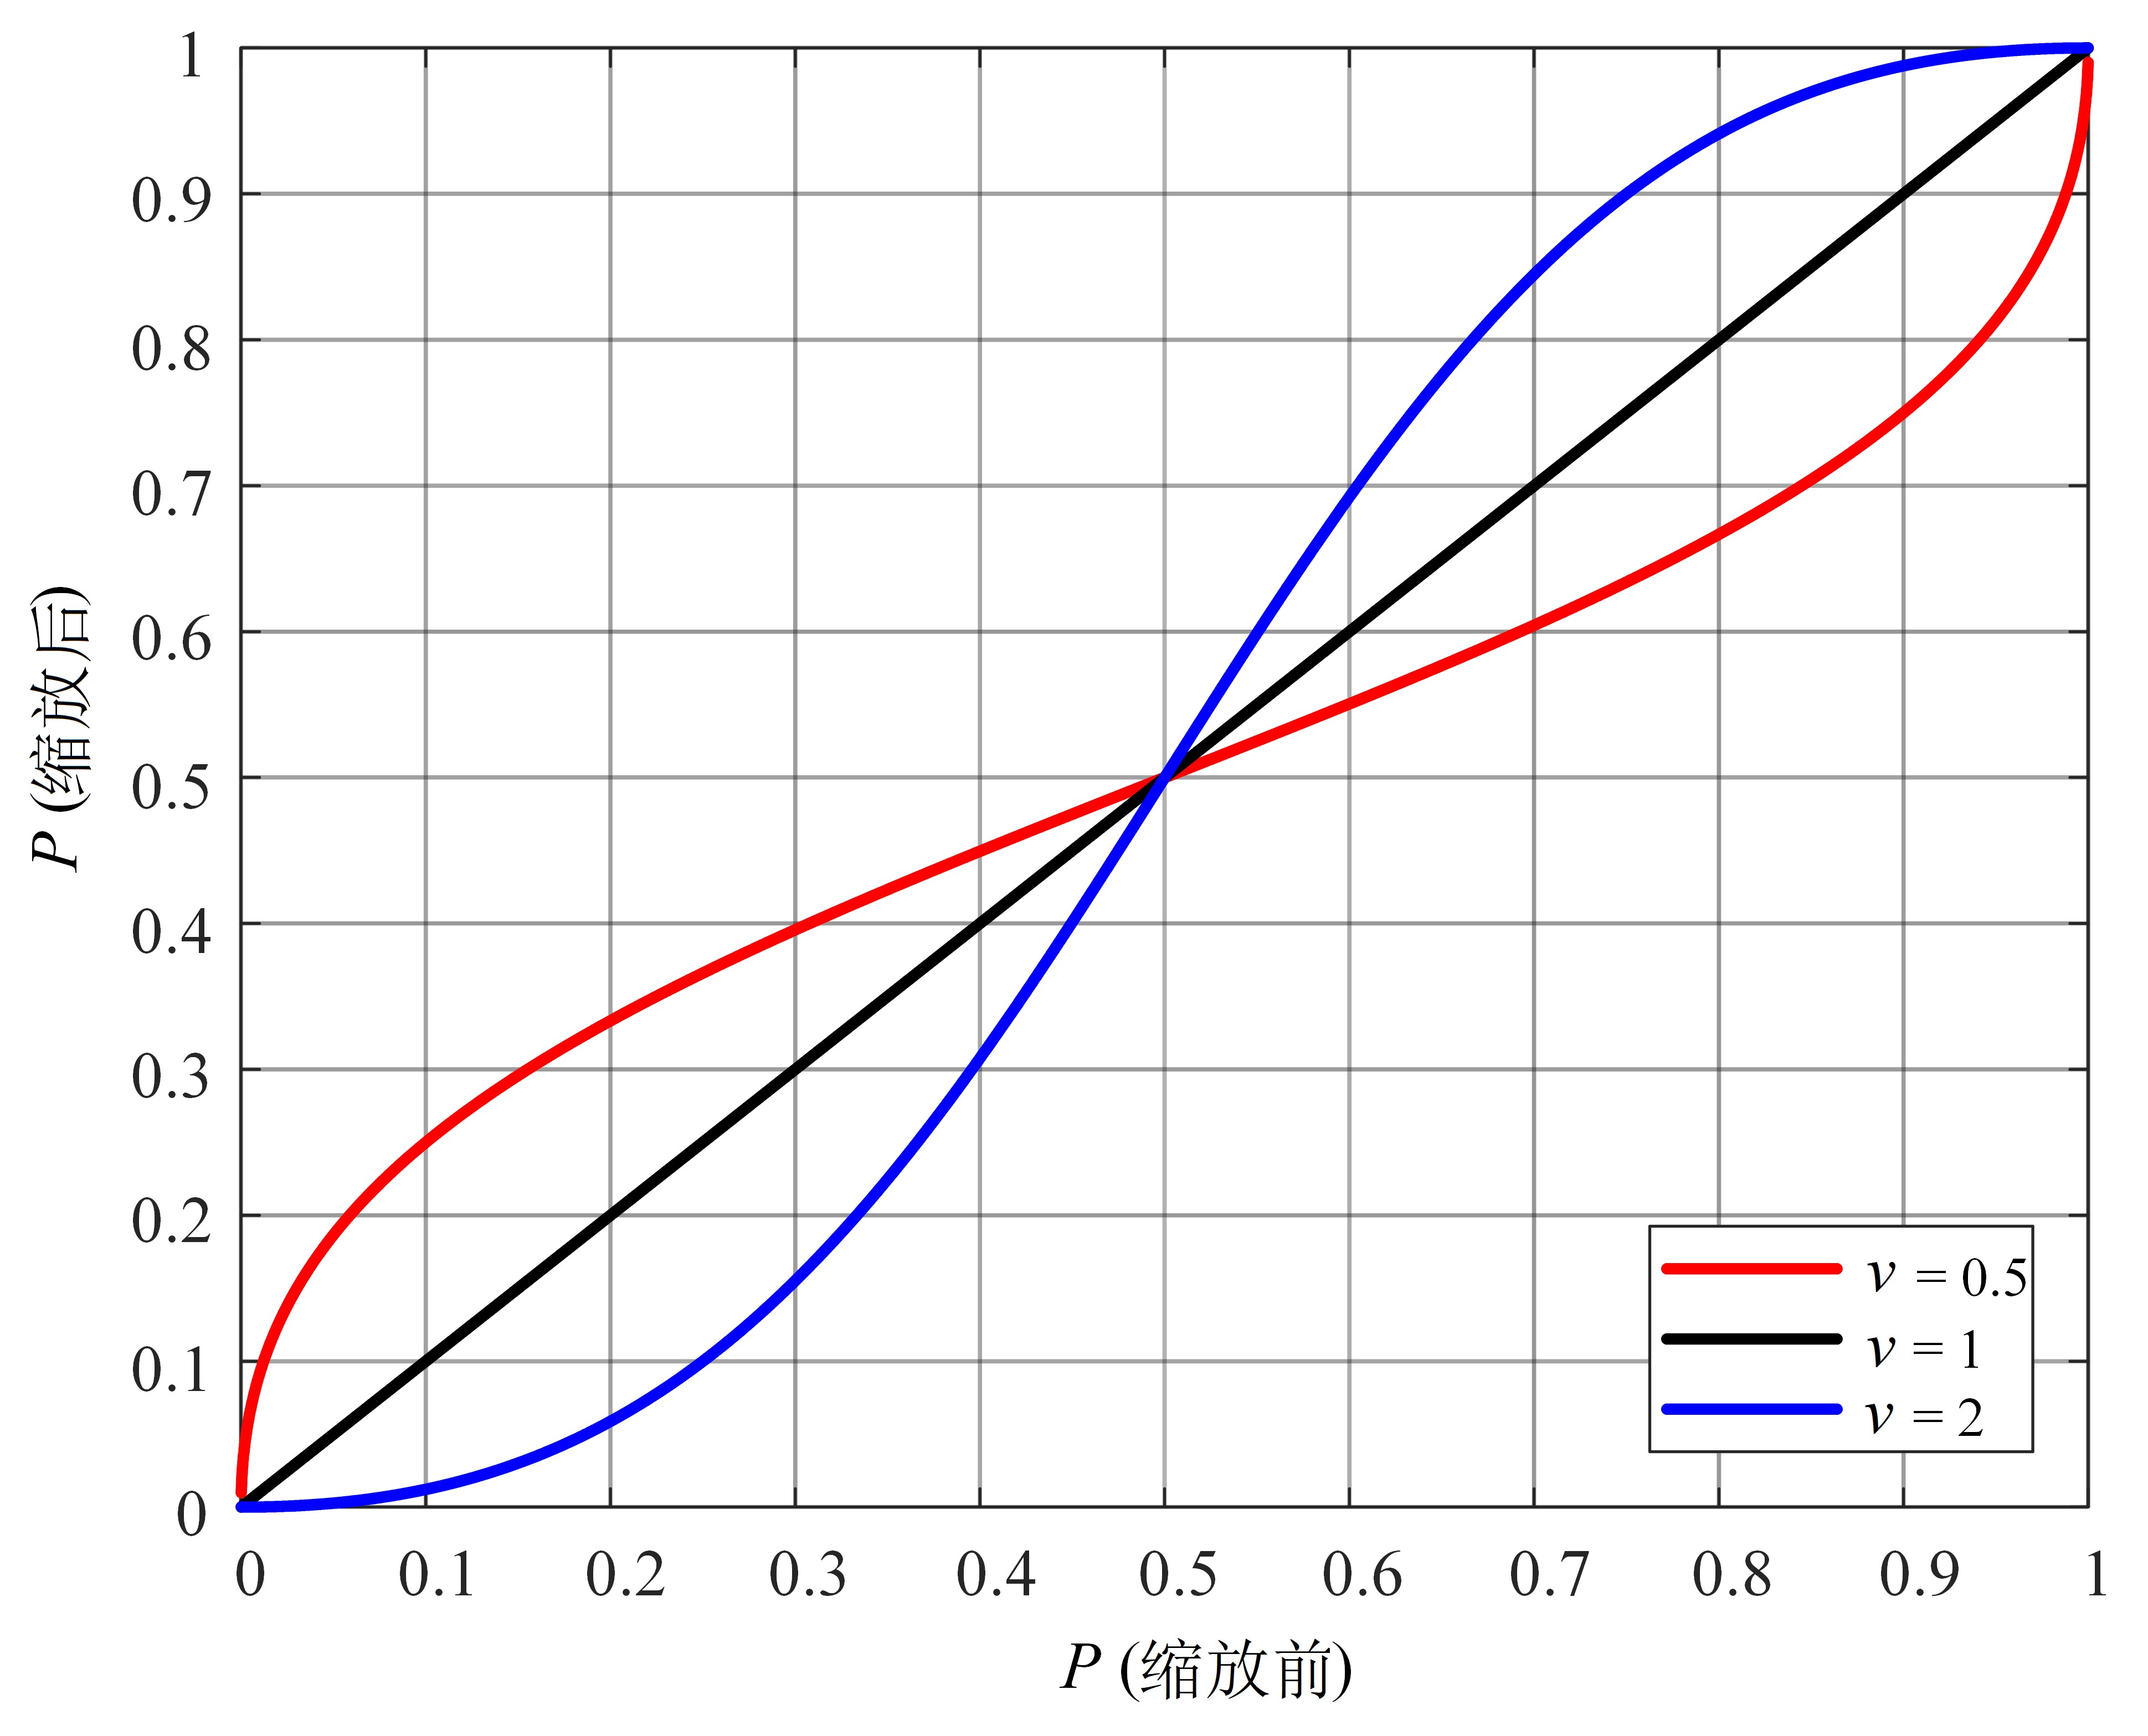
\includegraphics[width=10cm]{chapters/31}
	    \bicaption[\xiaosi 不同缩放系数v的缩放效果]{\wuhao 不同缩放系数v的缩放结果}{\wuhao Scaling results with different scaling coefficients ν}
	   	 \label{fig:3.1}
\end{figure}

%调整图片与下方文字之间的间距
\vspace{-0.35cm}

图片标题与图片之间的间距使用默认设置即可,与上下文的间距由于LATEX动态排版特性,需要大家手动调整。

。

。

。

。

。

。

。

。



下图是多子图示例:
%\vspace{-1cm}



\begin{figure}[h]
	\centering
	\subfigure[]{
		\label{fig:DE_J}
		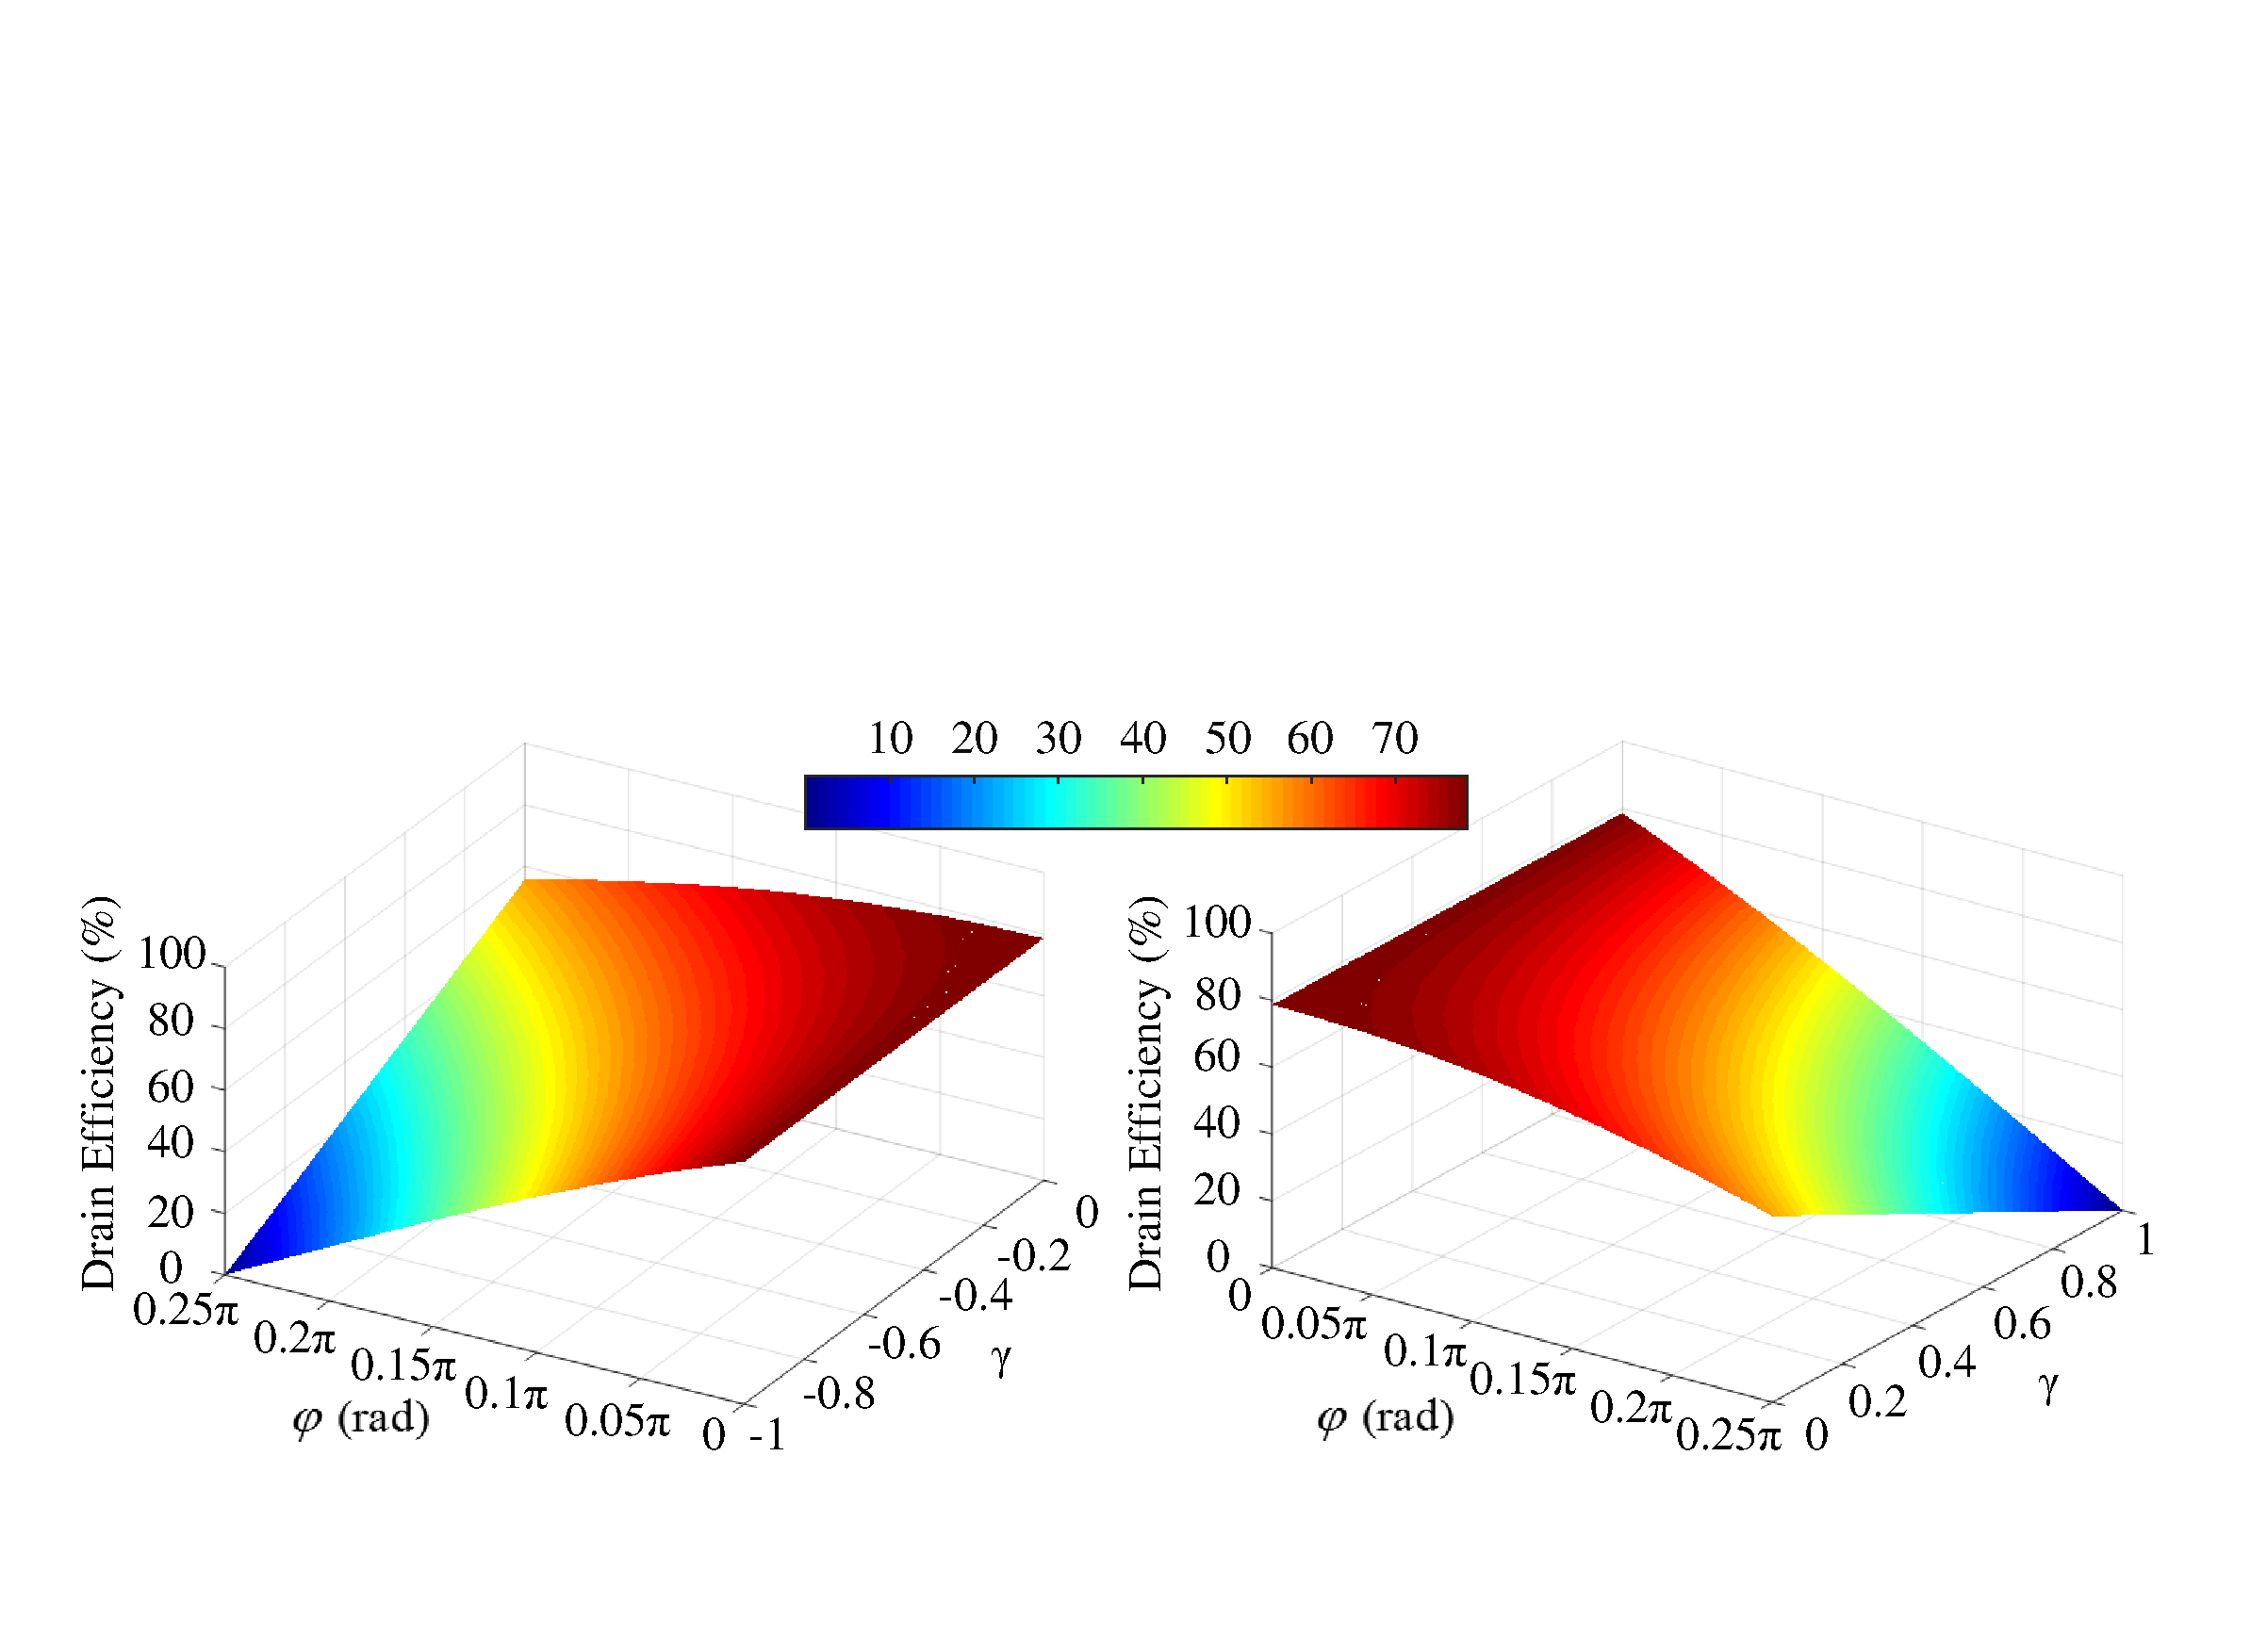
\includegraphics[width=12cm]{chapters/DE_J.pdf}}
	\subfigure[]{
		\label{fig:DE_CF}
		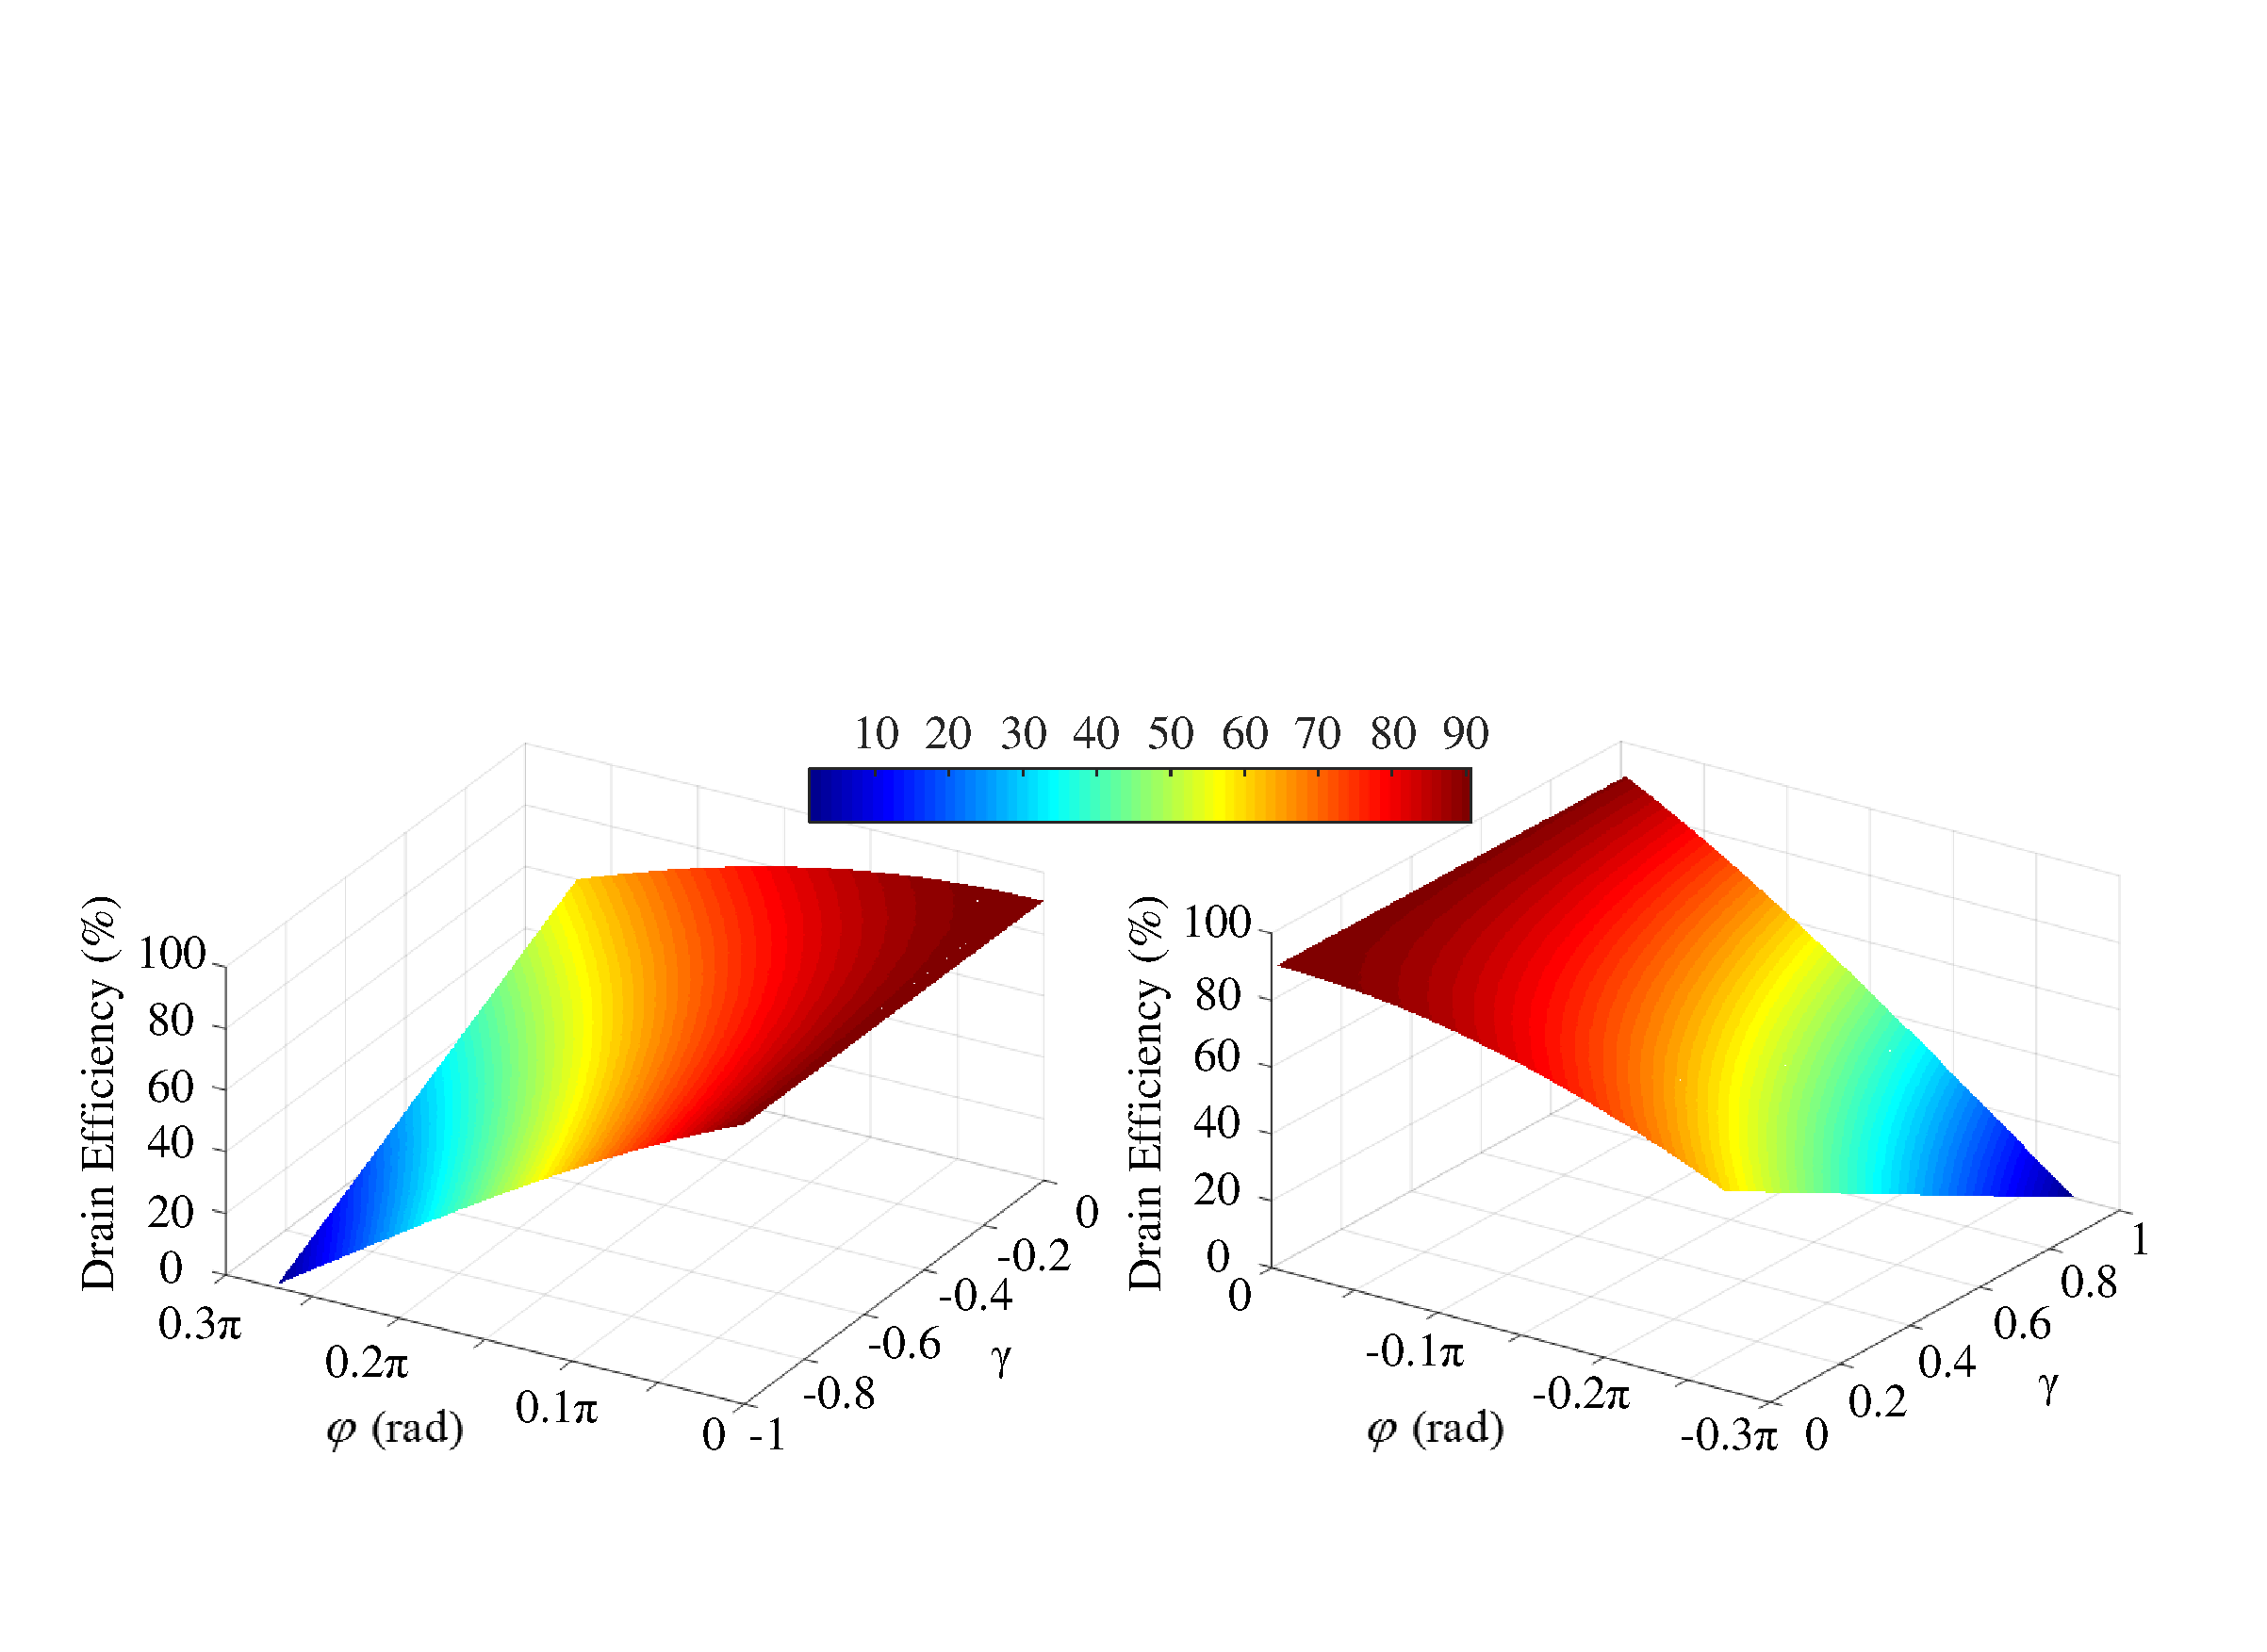
\includegraphics[width=12cm]{chapters/DE_CF.pdf}}   
\bicaption[\xiaosi 理论效率与$\gamma$和$\varphi$的关系。]{\wuhao 理论效率与$\gamma$和$\varphi$的关系。 (a) $\alpha=1$; (b) $\alpha=2/\sqrt{3}$}{\wuhao Theoretical DE versus $\gamma$ and $\varphi$. (a) $\alpha=1$; (b) $\alpha=2/\sqrt{3}$}

%	\caption{\wuhao 理论效率与$\gamma$和$\varphi$的关系。 (a) $\alpha=1$; (b) $\alpha=2/\sqrt{3}$}
%%	\raggedright
%	\wuhao Fig. 3-2 Theoretical DE versus $\gamma$ and $\varphi$. (a) $\alpha=1$. (b) $\alpha=2/\sqrt{3}$.Theoretical DE versus $\gamma$ and $\varphi$. (a) $\alpha=1$. (b) $\alpha=2/\sqrt{3}$.
\end{figure}

\vspace{-0.5cm}

\subsection{表}

表格格式参照写作指南。表格格式参照写作指南。表格格式参照写作指南。表格格式参照写作指南。表格格式参照写作指南。表格格式参照写作指南。表格格式参照写作指南。表格格式参照写作指南。表格格式参照写作指南。表格格式参照写作指南。表格格式参照写作指南。表格格式参照写作指南。表格格式参照写作指南。表格格式参照写作指南。表格格式参照写作指南。表格格式参照写作指南。

\vspace{0.1cm}

\begin{table}[h]
	\renewcommand{\arraystretch}{1.5}
	\centering
	\bicaption[\xiaosi 电流类型对效率的影响]{\wuhao 电流类型对效率的影响}{\wuhao Current type impact on efficiency}
	\begin{tabular}{p{3cm}p{3cm}p{3cm}p{3cm}}
		\toprule[1.5pt]
		\makecell[c]{\songti\wuhao 电流类型}&\makecell[c]{\songti\wuhao A}&\makecell[c]{\songti\wuhao B}&\makecell[c]{\songti\wuhao C}\\
		\hline
		\makecell[c]{\wuhao aaa}&\makecell[c]{\wuhao aa1}&\makecell[c]{\wuhao bb1}&\makecell[c]{\wuhao cc1}\\
		\bottomrule[1.5pt]
	\end{tabular}
   \label{tab:3.1} 	
\end{table}

表格格式参照写作指南。表格格式参照写作指南。表格格式参照写作指南。表格格式参照写作指南。表格格式参照写作指南。表格格式参照写作指南。表格格式参照写作指南。表格格式参照写作指南。表格格式参照写作指南。表格格式参照写作指南。表格格式参照写作指南。表格格式参照写作指南。表格格式参照写作指南。表格格式参照写作指南。表格格式参照写作指南。表格格式参照写作指南。

\vspace{-0.1cm}

\begin{table*}[h]
	\renewcommand{\arraystretch}{1.5}
	\bicaption[\xiaosi 高效率功放性能对比]{\wuhao 高效率功放性能对比}{\wuhao High-effiency power amplifier performance comparison}
	\label{tab_1}
	\centering
	\wuhao
	\begin{tabular}{c c c c c }
		\hline
		{\textbf{带宽}(GHz)}&{\textbf{功率}(dBm)}&{\textbf{效率}(\%)}&{\textbf{线性度}(dBc)}&{\textbf{信号带宽}(MHz)}\\
		\hline
		1.4--2.6&32--34&30--40 (DE)&-25 -- -30 (ACLR)&5\\
		\hline
		\multirow{2}{*}{2.1--2.7}&39&45 (DE) @ 2.14 GHz&--31 (ACLR)&\multirow{2}{*}{5}\\\cline{3-4}
		&(average)&40 (DE) @ 2.655 GHz&--30 (ACLR)&\\
		\hline
		3.5&38.1&59 (PAE)&30 (C/I)&5\\
		\hline
		\multirow{2}{*}{1.6--2.6}&36.0--38.5&45--60 (PAE)&30 (C/I)&5\\\cline{2-5}
		&35.3--37.5&40--55 (PAE)&--30 (ACLR)&20\\
		\hline
	\end{tabular}
\end{table*}


\section{公式格式}

\begin{equation}
\left\{ \begin{aligned}
0.794 \le \zeta  \le 1 ~~~~~~~~~~~\\
0.631 \le \gamma  = \frac{{0.631}}{{{\zeta ^2}}} \le 1~~~~~~ \\
- \frac{1}{{2\gamma }} \le \delta  \le \frac{1}{{2\gamma }}~~~~~~~~~~~ \\
{Z_{c,low,f}} = 2{R_{opt}}(\gamma  + j\delta )~~~~~\\
{Z_{c,2f}} = {Z_{c,low,2f}} =  - j\frac{{3\pi }}{4}\gamma \delta {R_{opt}}
\end{aligned} \right.
\label{eq:3.1}
\end{equation}

\begin{equation}
\begin{aligned}
v(\theta ) = V_{DD}\cdot(1 - \alpha cos(\theta  + \varphi ) + \beta cos(3\theta  + 3\varphi ))\\
\cdot(1 - \gamma \sin (\theta  + \varphi )) ~~~~~- 1 \le \gamma  \le 1\
\end{aligned}
\label{eq:vd}
\end{equation}




\noindent
公式格式测试。${\mathbf{\Theta }} = \left\{ {{\theta _k}\left( n \right),\forall k,n} \right\}$

\section{印制要求}
涉密学位论文的印刷、制作、传递、存档等,须符合国家、学校相关保密要求。学位论文一律左侧装订。

中文摘要之前的前置部分(封面、中、英文题名页、独创性声明和使用授权书),采用单面印刷。

从中文摘要开始,采用双面印刷。

中文摘要及之后的前置部分,包括中文摘要、ABSTRACT、目录、图目录(如有)、表目录(如有)、主要符号表(如有)、缩略词表(如有),在双面印刷时,若某部分页数为奇数,则该部分最后一页单面印刷。例如:若“摘要”只有1页,则其页码是“Ⅰ”,第“Ⅰ”页纸的背面为空白(无页眉或页码);“ABSTRACT”用新的一张纸印刷,页码从“Ⅱ”开始。

从第1章第1页开始,至论文最后1页,所有页面均双面印刷。例如:若第1章的最后1页为第17页,则第2章的第1页在第17页的背面印刷,页码为“18”(页眉是“重庆邮电大学博士(硕士)学位论文”)。

一次性双面打印整本学位论文技巧:除用于打印的版本外,电子版论文中一律不得出现空白页。论文打印建议使用PDF格式。为方便一次性双面打印,有时可在单面印刷的部分(如封面、中、英文题名页、独创性声明和使用授权书),或者双面打印只有1页的某部分内容(如摘要、ABSTRACT等)后插入1页空白页,该空白页不编排页眉页码;论文中出现的页码应前后连续,不得中断。


\section{本章小结}
本章介绍了……
\backmatter

%取消后续章节的页眉上的章节编号
\renewcommand{\chaptermark}[1]{\markboth{#1}{}}

%参考文献
% %参考文献
% \begin{thebibliography}{200}
% \wuhao %设置参考文献字体大小
% \linespread{1}\selectfont
% \setlength{\itemsep}{-1.4ex} %缩小条目间行距
% \thispagestyle{others}
% \pagestyle{others}

% \makeatletter
% \renewcommand\@biblabel[1]{[#1]\hfill} %序号左对齐
% \makeatother
% \setlength{\labelsep}{0cm}

%   \providecommand{\bibauthor}[1]{#1}
%   \providecommand{\bibeditor}[1]{#1}
%   \providecommand{\bibtranslator}[1]{#1}
%   \providecommand{\bibtitle}[1]{#1}
%   \providecommand{\bibbooktitle}[1]{#1}
%   \providecommand{\bibjournal}[1]{#1}
%   \providecommand{\bibmark}[1]{#1}
%   \providecommand{\bibcountry}[1]{#1}
%   \providecommand{\bibpatentid}[1]{#1}
%   \providecommand{\bibedition}[1]{#1}
%   \providecommand{\biborganization}[1]{#1}
%   \providecommand{\bibaddress}[1]{#1}
%   \providecommand{\bibpublisher}[1]{#1}
%   \providecommand{\bibinstitution}[1]{#1}
%   \providecommand{\bibschool}[1]{#1}
%   \providecommand{\bibvolume}[1]{#1}
%   \providecommand{\bibnumber}[1]{#1}
%   \providecommand{\bibpages}[1]{#1}
%   \providecommand{\bibmodifydate}[1]{#1}
%   \providecommand{\bibcitedate}[1]{#1}
%   \providecommand{\bibyear}[1]{#1}
%   \providecommand{\bibdate}[1]{#1}
%   \providecommand{\biburl}[1]{\url{#1}}
  
%   \bibitem{PointNetVLAD}
%   \bibauthor{UY M~A\@, LEE G~H}\@. \bibtitle{PointNetVLAD: Deep point cloud based
%     retrieval for large-scale place recognition}\bibmark{[C]}\@.
%     \bibbooktitle{IEEE/CVF Conference on Computer Vision and Pattern
%     Recognition}\@, \bibaddress{Salt Lake City, USA}\@,
%     \bibyear{2018}\thinspace{}\textnormal{:
%     }\bibpages{4470\thinspace{}\textnormal{--}\thinspace{}4479}\@.
  
%   \bibitem{文物}
%   \bibauthor{赵夫群\@, 周明全}\@.
%     \bibtitle{文物点云模型的优化配准算法}\bibmark{[J]}\@.
%     \bibjournal{计算机应用研究}\@, \bibyear{2017}\@,
%     \bibvolume{34}\bibnumber{(12)}\thinspace{}\textnormal{: }\bibpages{4}\@.
  
%   \bibitem{逆向工程}
%   \bibauthor{宋丽梅}\@.
%     \bibtitle{双目立体机器视觉检测系统及其应用}\bibmark{[J]}\@.
%     \bibjournal{西南科技大学学报}\@, \bibyear{2006}\@,
%     \bibvolume{21}\bibnumber{(1)}\thinspace{}\textnormal{:
%     }\bibpages{30\thinspace{}\textnormal{--}\thinspace{}34}\@.
  
%   \bibitem{Map-matching}
%   \bibauthor{SOBREIRA H\@, COSTA C~M\@, SOUSA I, et~al}\@. \bibtitle{Map-matching
%     algorithms for robot self-localization: a comparison between perfect match,
%     iterative closest point and normal distributions transform}\bibmark{[J]}\@.
%     \bibjournal{Intelligent \& Robotic Systems}\@, \bibyear{2019}\@,
%     \bibvolume{93}\thinspace{}\textnormal{:
%     }\bibpages{533\thinspace{}\textnormal{--}\thinspace{}546}\@.
  
%   \bibitem{LCDNet}
%   \bibauthor{CATTANEO D\@, VAGHI M\@, VALADA A}\@. \bibtitle{LCDNet: Deep loop
%     closure detection and point cloud registration for LiDAR
%     SLAM}\bibmark{[J]}\@. \bibjournal{IEEE Transactions on Robotics}\@,
%     \bibyear{2022}\@, \bibvolume{38}\bibnumber{(4)}\thinspace{}\textnormal{:
%     }\bibpages{2074\thinspace{}\textnormal{--}\thinspace{}2093}\@.
  
%   \bibitem{LPD}
%   \bibauthor{LIU Z\@, ZHOU S\@, SUO C, et~al}\@. \bibtitle{LPD-Net: 3D point
%     cloud learning for large-scale place recognition and environment
%     analysis}\bibmark{[C]}\@. \bibbooktitle{IEEE/CVF International Conference on
%     Computer Vision}\@, \bibaddress{Seoul, Korea}\@,
%     \bibyear{2019}\thinspace{}\textnormal{:
%     }\bibpages{2831\thinspace{}\textnormal{--}\thinspace{}2840}\@.
  
%   \bibitem{2015review}
%   \bibauthor{POMERLEAU F\@, COLAS F\@, SIEGWART R, et~al}\@. \bibtitle{A review
%     of point cloud registration algorithms for mobile robotics}\bibmark{[J]}\@.
%     \bibjournal{Foundations and Trends{\textregistered} in Robotics}\@,
%     \bibyear{2015}\@, \bibvolume{4}\bibnumber{(1)}\thinspace{}\textnormal{:
%     }\bibpages{1\thinspace{}\textnormal{--}\thinspace{}104}\@.
  
%   \bibitem{ICP}
%   \bibauthor{BESL P\@, MCKAY N~D}\@. \bibtitle{A method for registration of 3-D
%     shapes}\bibmark{[J]}\@. \bibjournal{IEEE Transactions on Pattern Analysis and
%     Machine Intelligence}\@, \bibyear{1992}\@,
%     \bibvolume{14}\bibnumber{(2)}\thinspace{}\textnormal{:
%     }\bibpages{239\thinspace{}\textnormal{--}\thinspace{}256}\@.
  
%   \bibitem{1998}
%   \bibauthor{GOLD S\@, RANGARAJAN A\@, LU C-P, et~al}\@. \bibtitle{New algorithms
%     for 2D and 3D point matching: pose estimation and
%     correspondence}\bibmark{[J]}\@. \bibjournal{Pattern Recognition}\@,
%     \bibyear{1998}\@, \bibvolume{31}\bibnumber{(8)}\thinspace{}\textnormal{:
%     }\bibpages{1019\thinspace{}\textnormal{--}\thinspace{}1031}\@.
  
%   \bibitem{Go-ICP}
%   \bibauthor{YANG J\@, LI H\@, JIA Y}\@. \bibtitle{Go-ICP: Solving 3D
%     registration efficiently and globally optimally}\bibmark{[C]}\@.
%     \bibbooktitle{IEEE/CVF International Conference on Computer Vision}\@,
%     \bibaddress{Sydney, Australia}\@, \bibyear{2013}\thinspace{}\textnormal{:
%     }\bibpages{1457\thinspace{}\textnormal{--}\thinspace{}1464}\@.
  
%   \bibitem{Almohamad}
%   \bibauthor{ALMOHAMAD H\@, DUFFUAA S~O}\@. \bibtitle{A linear programming
%     approach for the weighted graph matching problem}\bibmark{[J]}\@.
%     \bibjournal{IEEE Transactions on pattern analysis and machine
%     intelligence}\@, \bibyear{1993}\@,
%     \bibvolume{15}\bibnumber{(5)}\thinspace{}\textnormal{:
%     }\bibpages{522\thinspace{}\textnormal{--}\thinspace{}525}\@.
  
%   \bibitem{CSGM}
%   \bibauthor{HUANG X\@, ZHANG J\@, FAN L, et~al}\@. \bibtitle{A systematic
%     approach for cross-source point cloud registration by preserving macro and
%     micro structures}\bibmark{[J]}\@. \bibjournal{IEEE Transactions on Image
%     Processing}\@, \bibyear{2017}\@,
%     \bibvolume{26}\bibnumber{(7)}\thinspace{}\textnormal{:
%     }\bibpages{3261\thinspace{}\textnormal{--}\thinspace{}3276}\@.
  
%   \bibitem{FGM}
%   \bibauthor{ZHOU F\@, De~la TORRE F}\@. \bibtitle{Factorized graph
%     matching}\bibmark{[C]}\@. \bibbooktitle{IEEE/CVF Conference on Computer
%     Vision and Pattern Recognition}\@, \bibaddress{Providence, USA}\@,
%     \bibyear{2012}\thinspace{}\textnormal{:
%     }\bibpages{127\thinspace{}\textnormal{--}\thinspace{}134}\@.
  
%   \bibitem{Leordeanu}
%   \bibauthor{LEORDEANU M\@, HEBERT M}\@. \bibtitle{A spectral technique for
%     correspondence problems using pairwise constraints}\bibmark{[C]}\@.
%     \bibbooktitle{IEEE/CVF International Conference on Computer Vision}\@,
%     \bibaddress{Beijing, China}\@, \bibyear{2005}\thinspace{}\textnormal{:
%     }\bibpages{1482\thinspace{}\textnormal{--}\thinspace{}1489}\@.
  
%   \bibitem{JRMPC}
%   \bibauthor{EVANGELIDIS G~D\@, KOUNADES-BASTIAN D\@, HORAUD R, et~al}\@.
%     \bibtitle{A generative model for the joint registration of multiple point
%     sets}\bibmark{[C]}\@. \bibbooktitle{European Conference on Computer
%     Vision}\@, \bibaddress{Zurich, Switzerland}\@, \bibyear{2014}\@.
  
%   \bibitem{CPD}
%   \bibauthor{MYRONENKO A\@, SONG X}\@. \bibtitle{Point set registration: coherent
%     point drift}\bibmark{[J]}\@. \bibjournal{IEEE Transactions on Pattern
%     Analysis and Machine Intelligence}\@, \bibyear{2010}\@,
%     \bibvolume{32}\bibnumber{(12)}\thinspace{}\textnormal{:
%     }\bibpages{2262\thinspace{}\textnormal{--}\thinspace{}2275}\@.
  
%   \bibitem{CH-GMM}
%   \bibauthor{FAN J\@, YANG J\@, AI D, et~al}\@. \bibtitle{Convex hull indexed
%     Gaussian mixture model for 3D point set registration}\bibmark{[J]}\@.
%     \bibjournal{Pattern Recognition}\@, \bibyear{2016}\@,
%     \bibvolume{59}\thinspace{}\textnormal{:
%     }\bibpages{126\thinspace{}\textnormal{--}\thinspace{}141}\@.
  
%   \bibitem{PointNetLK}
%   \bibauthor{AOKI Y\@, GOFORTH H\@, SRIVATSAN R~A, et~al}\@.
%     \bibtitle{PointNetLK: robust \& efficient point cloud registration ssing
%     pointNet}\bibmark{[C]}\@. \bibbooktitle{IEEE/CVF Conference on Computer
%     Vision and Pattern Recognition}\@, \bibaddress{Seoul, Korea}\@,
%     \bibyear{2019}\thinspace{}\textnormal{:
%     }\bibpages{7156\thinspace{}\textnormal{--}\thinspace{}7165}\@.
  
%   \bibitem{LucasKanade}
%   \bibauthor{BAKER S\@, MATTHEWS I}\@. \bibtitle{Lucas-Kanade 20 years on: A
%     unifying framework}\bibmark{[J]}\@. \bibjournal{International Journal of
%     Computer Vision}\@, \bibyear{2004}\@, \bibvolume{56}\thinspace{}\textnormal{:
%     }\bibpages{221\thinspace{}\textnormal{--}\thinspace{}255}\@.
  
%   \bibitem{PPF}
%   \bibauthor{DENG H\@, BIRDAL T\@, ILIC S}\@. \bibtitle{PPFNet: Global context
%     aware local features for robust 3D point matching}\bibmark{[C]}\@.
%     \bibbooktitle{IEEE/CVF Conference on Computer Vision and Pattern
%     Recognition}\@, \bibaddress{Salt Lake City, USA}\@,
%     \bibyear{2018}\thinspace{}\textnormal{:
%     }\bibpages{195\thinspace{}\textnormal{--}\thinspace{}205}\@.
  
%   \bibitem{FMR}
%   \bibauthor{HUANG X\@, MEI G\@, ZHANG J}\@. \bibtitle{Feature-Metric
%     registration: A fast semi-Supervised approach for robust point cloud
%     registration without correspondences}\bibmark{[C]}\@. \bibbooktitle{IEEE/CVF
%     Conference on Computer Vision and Pattern Recognition}\@,
%     \bibaddress{Seattle, USA}\@, \bibyear{2020}\thinspace{}\textnormal{:
%     }\bibpages{11363\thinspace{}\textnormal{--}\thinspace{}11371}\@.
  
%   \bibitem{OMNet}
%   \bibauthor{XU H\@, LIU S\@, WANG G, et~al}\@. \bibtitle{OMNet: Learning
%     overlapping mask for partial-to-partial point cloud
%     registration}\bibmark{[C]}\@. \bibbooktitle{IEEE/CVF International Conference
%     on Computer Vision}\@, \bibaddress{Montreal, Canada}\@,
%     \bibyear{2021}\thinspace{}\textnormal{:
%     }\bibpages{3112\thinspace{}\textnormal{--}\thinspace{}3121}\@.
  
%   \bibitem{PointNet}
%   \bibauthor{CHARLES R~Q\@, SU H\@, KAICHUN M, et~al}\@. \bibtitle{PointNet: Deep
%     learning on point sets for 3D classification and
%     segmentation}\bibmark{[C]}\@. \bibbooktitle{IEEE/CVF Conference on Computer
%     Vision and Pattern Recognition}\@, \bibaddress{Honolulu, USA}\@,
%     \bibyear{2017}\thinspace{}\textnormal{:
%     }\bibpages{77\thinspace{}\textnormal{--}\thinspace{}85}\@.
  
%   \bibitem{PointNet++}
%   \bibauthor{QI R\@, YI L\@, SU H, et~al}\@. \bibtitle{Pointnet++: Deep
%     hierarchical feature learning on point sets in a metric
%     space}\bibmark{[J]}\@. \bibjournal{Advances in Neural Information Processing
%     Systems}\@, \bibyear{2017}\@, \bibvolume{30}\thinspace{}\textnormal{:
%     }\bibpages{5099\thinspace{}\textnormal{--}\thinspace{}5108}\@.
  
%   \bibitem{3DFeat-Net}
%   \bibauthor{YEW Z~J\@, LEE G~H}\@. \bibtitle{3DFeat-Net: Weakly supervised local
%     3D features for point cloud registration}\bibmark{[C]}\@.
%     \bibbooktitle{European Conference on Computer Vision}\@, \bibaddress{Munich,
%     Germany}\@, \bibyear{2018}\thinspace{}\textnormal{:
%     }\bibpages{630\thinspace{}\textnormal{--}\thinspace{}646}\@.
  
%   \bibitem{PerfectMatch}
%   \bibauthor{GOJCIC Z\@, ZHOU C\@, WEGNER J~D, et~al}\@. \bibtitle{The Perfect
%     Match: 3D Point Cloud Matching With Smoothed Densities}\bibmark{[C]}\@.
%     \bibbooktitle{IEEE/CVF Conference on Computer Vision and Pattern
%     Recognition}\@, \bibaddress{Long Beach, USA}\@,
%     \bibyear{2019}\thinspace{}\textnormal{:
%     }\bibpages{5540\thinspace{}\textnormal{--}\thinspace{}5549}\@.
  
%   \bibitem{DGCNN}
%   \bibauthor{WANG Y\@, SUN Y\@, LIU Z, et~al}\@. \bibtitle{Dynamic graph cnn for
%     learning on point clouds}\bibmark{[J]}\@. \bibjournal{Acm Transactions On
%     Graphics}\@, \bibyear{2019}\@,
%     \bibvolume{38}\bibnumber{(5)}\thinspace{}\textnormal{:
%     }\bibpages{1\thinspace{}\textnormal{--}\thinspace{}12}\@.
  
%   \bibitem{KPConv}
%   \bibauthor{THOMAS H\@, QI C~R\@, DESCHAUD J-E, et~al}\@. \bibtitle{KPConv:
%     Flexible and deformable convolution for point clouds}\bibmark{[C]}\@.
%     \bibbooktitle{IEEE/CVF International Conference on Computer Vision}\@,
%     \bibaddress{Seoul, Korea}\@, \bibyear{2019}\thinspace{}\textnormal{:
%     }\bibpages{6410\thinspace{}\textnormal{--}\thinspace{}6419}\@.
  
%   \bibitem{3DMatch}
%   \bibauthor{ZENG A\@, SONG S\@, NIEßNER M, et~al}\@. \bibtitle{3DMatch:
%     Learning local geometric descriptors from RGB-D
%     reconstructions}\bibmark{[C]}\@. \bibbooktitle{IEEE/CVF Conference on
%     Computer Vision and Pattern Recognition}\@, \bibaddress{Honolulu, USA}\@,
%     \bibyear{2017}\thinspace{}\textnormal{:
%     }\bibpages{199\thinspace{}\textnormal{--}\thinspace{}208}\@.
  
%   \bibitem{FCGF}
%   \bibauthor{CHOY C\@, PARK J\@, KOLTUN V}\@. \bibtitle{Fully convolutional
%     geometric features}\bibmark{[C]}\@. \bibbooktitle{IEEE/CVF International
%     Conference on Computer Vision}\@, \bibaddress{Seoul, Korea}\@,
%     \bibyear{2019}\thinspace{}\textnormal{:
%     }\bibpages{8957\thinspace{}\textnormal{--}\thinspace{}8965}\@.
  
%   \bibitem{SpinNet}
%   \bibauthor{AO S\@, HU Q\@, YANG B, et~al}\@. \bibtitle{Spinnet: Learning a
%     general surface descriptor for 3d point cloud registration}\bibmark{[C]}\@.
%     \bibbooktitle{IEEE/CVF Conference on Computer Vision and Pattern
%     Recognition}\@, \bibaddress{virtual}\@,
%     \bibyear{2021}\thinspace{}\textnormal{:
%     }\bibpages{11753\thinspace{}\textnormal{--}\thinspace{}11762}\@.
  
%   \bibitem{D3Feat}
%   \bibauthor{BAI X\@, LUO Z\@, ZHOU L, et~al}\@. \bibtitle{D3Feat: Joint learning
%     of dense detection and description of 3D local features}\bibmark{[C]}\@.
%     \bibbooktitle{IEEE/CVF Conference on Computer Vision and Pattern
%     Recognition}\@, \bibaddress{Seattle, USA}\@,
%     \bibyear{2020}\thinspace{}\textnormal{:
%     }\bibpages{6358\thinspace{}\textnormal{--}\thinspace{}6366}\@.
  
%   \bibitem{PREDATOR}
%   \bibauthor{HUANG S\@, GOJCIC Z\@, USVYATSOV M, et~al}\@. \bibtitle{PREDATOR:
%     Registration of 3D point clouds with low overlap}\bibmark{[C]}\@.
%     \bibbooktitle{IEEE/CVF Conference on Computer Vision and Pattern
%     Recognition}\@, \bibaddress{virtual}\@,
%     \bibyear{2021}\thinspace{}\textnormal{:
%     }\bibpages{4265\thinspace{}\textnormal{--}\thinspace{}4274}\@.
  
%   \bibitem{PointDSC}
%   \bibauthor{BAI X\@, LUO Z\@, ZHOU L, et~al}\@. \bibtitle{PointDSC: Robust point
%     cloud registration using deep spatial consistency}\bibmark{[C]}\@.
%     \bibbooktitle{IEEE/CVF Conference on Computer Vision and Pattern
%     Recognition}\@, \bibaddress{virtual}\@,
%     \bibyear{2021}\thinspace{}\textnormal{:
%     }\bibpages{15854\thinspace{}\textnormal{--}\thinspace{}15864}\@.
  
%   \bibitem{DCP}
%   \bibauthor{WANG Y\@, SOLOMON J}\@. \bibtitle{Deep Closest Point: Learning
%     representations for point cloud registration}\bibmark{[C]}\@.
%     \bibbooktitle{IEEE/CVF International Conference on Computer Vision}\@,
%     \bibaddress{Seoul, Korea}\@, \bibyear{2019}\thinspace{}\textnormal{:
%     }\bibpages{3522\thinspace{}\textnormal{--}\thinspace{}3531}\@.
  
%   \bibitem{IDAM}
%   \bibauthor{LI J\@, ZHANG C\@, XU Z, et~al}\@. \bibtitle{Iterative
%     distance-aware similarity matrix convolution with mutual-supervised point
%     elimination for efficient point cloud registration}\bibmark{[C]}\@.
%     \bibbooktitle{European Conference on Computer Vision}\@, \bibaddress{Glasgow,
%     UK}\@, \bibyear{2020}\thinspace{}\textnormal{:
%     }\bibpages{378\thinspace{}\textnormal{--}\thinspace{}394}\@.
  
%   \bibitem{DGR}
%   \bibauthor{CHOY C\@, DONG W\@, KOLTUN V}\@. \bibtitle{Deep global
%     registration}\bibmark{[C]}\@. \bibbooktitle{IEEE/CVF Conference on Computer
%     Vision and Pattern Recognition}\@, \bibaddress{Seattle, USA}\@,
%     \bibyear{2020}\thinspace{}\textnormal{:
%     }\bibpages{2511\thinspace{}\textnormal{--}\thinspace{}2520}\@.
  
%   \bibitem{Dope}
%   \bibauthor{MIN T\@, SONG C\@, KIM E, et~al}\@. \bibtitle{Distinctiveness
%     oriented positional equilibrium for point cloud registration}\bibmark{[C]}\@.
%     \bibbooktitle{IEEE/CVF International Conference on Computer Vision}\@,
%     \bibaddress{Montreal, Canada}\@, \bibyear{2021}\thinspace{}\textnormal{:
%     }\bibpages{5490\thinspace{}\textnormal{--}\thinspace{}5498}\@.
  
%   \bibitem{Deeper}
%   \bibauthor{LI Q\@, HAN Z\@, WU X-M}\@. \bibtitle{Deeper Insights into Graph
%     Convolutional Networks for Semi-Supervised Learning}\bibmark{[C]}\@.
%     \bibbooktitle{Proceedings of the AAAI Conference on Artificial
%     Intelligence}\@, \bibaddress{New Orleans, USA}\@,
%     \bibyear{2018}\thinspace{}\textnormal{:
%     }\bibpages{3538\thinspace{}\textnormal{--}\thinspace{}3545}\@.
  
%   \bibitem{Measuring}
%   \bibauthor{CHEN D\@, LIN Y\@, LI W, et~al}\@. \bibtitle{Measuring and relieving
%     the over-smoothing problem for graph neural networks from the topological
%     view}\bibmark{[J]}\@. \bibjournal{Proceedings of the AAAI Conference on
%     Artificial Intelligence}\@, \bibyear{2020}\@,
%     \bibvolume{34}\bibnumber{(04)}\thinspace{}\textnormal{:
%     }\bibpages{3438\thinspace{}\textnormal{--}\thinspace{}3445}\@.
  
%   \bibitem{RANSAC}
%   \bibauthor{FISCHLER M~A\@, BOLLES R~C}\@. \bibtitle{Random sample consensus: a
%     paradigm for model fitting with applications to image analysis and automated
%     cartography}\bibmark{[J]}\@. \bibjournal{Communications of the ACM}\@,
%     \bibyear{1981}\@, \bibvolume{24}\bibnumber{(6)}\thinspace{}\textnormal{:
%     }\bibpages{381\thinspace{}\textnormal{--}\thinspace{}395}\@.
  
%   \bibitem{Temporal}
%   \bibauthor{YUAN Z\@, SONG X\@, BAI L, et~al}\@. \bibtitle{Temporal-channel
%     transformer for 3d lidar-based video object detection for autonomous
%     driving}\bibmark{[J]}\@. \bibjournal{IEEE Transactions on Circuits and
%     Systems for Video Technology}\@, \bibyear{2021}\@,
%     \bibvolume{32}\bibnumber{(4)}\thinspace{}\textnormal{:
%     }\bibpages{2068\thinspace{}\textnormal{--}\thinspace{}2078}\@.
  
%   \bibitem{L3Net}
%   \bibauthor{LU W\@, ZHOU Y\@, WAN G, et~al}\@. \bibtitle{L3-Net: Towards
%     learning based LiDAR localization for autonomous driving}\bibmark{[C]}\@.
%     \bibbooktitle{IEEE/CVF Conference on Computer Vision and Pattern
%     Recognition}\@, \bibaddress{Long Beach, USA}\@,
%     \bibyear{2019}\thinspace{}\textnormal{:
%     }\bibpages{6382\thinspace{}\textnormal{--}\thinspace{}6391}\@.
  
%   \bibitem{IMLSSLAM}
%   \bibauthor{DESCHAUD J-E}\@. \bibtitle{IMLS-SLAM: Scan-to-Model matching based
%     on 3D data}\bibmark{[C]}\@. \bibbooktitle{IEEE International Conference on
%     Robotics and Automation}\@, \bibaddress{Brisbane, Australia}\@,
%     \bibyear{2018}\thinspace{}\textnormal{:
%     }\bibpages{2480\thinspace{}\textnormal{--}\thinspace{}2485}\@.
  
%   \bibitem{Positioning}
%   \bibauthor{BENEDEK C\@, MAJDIK A\@, NAGY B, et~al}\@. \bibtitle{Positioning and
%     perception in LiDAR point clouds}\bibmark{[J]}\@. \bibjournal{Digital Signal
%     Processing}\@, \bibyear{2021}\@, \bibvolume{119}\thinspace{}\textnormal{:
%     }\bibpages{103193}\@.
  
%   \bibitem{Generative_Adversarial}
%   \bibauthor{TAN L\@, LIN X\@, NIU D, et~al}\@. \bibtitle{Projected generative
%     adversarial network for point cloud completion}\bibmark{[J]}\@.
%     \bibjournal{IEEE Transactions on Circuits and Systems for Video
%     Technology}\@, \bibyear{2023}\@,
%     \bibvolume{33}\bibnumber{(2)}\thinspace{}\textnormal{:
%     }\bibpages{771\thinspace{}\textnormal{--}\thinspace{}781}\@.
  
%   \bibitem{Single_Image}
%   \bibauthor{NGUYEN A-D\@, CHOI S\@, KIM W, et~al}\@. \bibtitle{Single-Image 3D
%     reconstruction: rethinking point cloud deformation}\bibmark{[J]}\@.
%     \bibjournal{IEEE Transactions on Neural Networks and Learning Systems}\@,
%     \bibyear{2022}\thinspace{}\textnormal{:
%     }\bibpages{1\thinspace{}\textnormal{--}\thinspace{}15}\@.
  
%   \bibitem{LPOT}
%   \bibauthor{WANG G}\@. \bibtitle{LPOT: Locality-Preserving gromov-wasserstein
%     discrepancy for nonrigid point set registration}\bibmark{[J]}\@.
%     \bibjournal{IEEE Transactions on Neural Networks and Learning Systems}\@,
%     \bibyear{2022}\thinspace{}\textnormal{:
%     }\bibpages{1\thinspace{}\textnormal{--}\thinspace{}13}\@.
  
%   \bibitem{Birds_Stone}
%   \bibauthor{GU C\@, CONG Y\@, SUN G}\@. \bibtitle{Three Birds, One Stone:
%     Unified laser-based 3D reconstruction across different media}\bibmark{[J]}\@.
%     \bibjournal{IEEE Transactions on Instrumentation and Measurement}\@,
%     \bibyear{2021}\@, \bibvolume{70}\thinspace{}\textnormal{:
%     }\bibpages{1\thinspace{}\textnormal{--}\thinspace{}12}\@.
  
%   \bibitem{INENet}
%   \bibauthor{WU Y\@, ZHANG Y\@, FAN X, et~al}\@. \bibtitle{INENet: Inliers
%     estimation network with similarity learning for partial overlapping
%     registration}\bibmark{[J]}\@. \bibjournal{IEEE Transactions on Circuits and
%     Systems for Video Technology}\@, \bibyear{2023}\@,
%     \bibvolume{33}\bibnumber{(3)}\thinspace{}\textnormal{:
%     }\bibpages{1413\thinspace{}\textnormal{--}\thinspace{}1426}\@.
  
%   \bibitem{Task_specific}
%   \bibauthor{ZHANG Z\@, DAI Y\@, FAN B, et~al}\@. \bibtitle{Learning a
%     task-specific descriptor for robust matching of 3D point
%     clouds}\bibmark{[J]}\@. \bibjournal{IEEE Transactions on Circuits and Systems
%     for Video Technology}\@, \bibyear{2022}\@,
%     \bibvolume{32}\bibnumber{(12)}\thinspace{}\textnormal{:
%     }\bibpages{8462\thinspace{}\textnormal{--}\thinspace{}8475}\@.
  
%   \bibitem{RANSAC_Hypotheses}
%   \bibauthor{YANG J\@, HUANG Z\@, QUAN S, et~al}\@. \bibtitle{Toward efficient
%     and robust metrics for RANSAC hypotheses and 3D rigid
%     registration}\bibmark{[J]}\@. \bibjournal{IEEE Transactions on Circuits and
%     Systems for Video Technology}\@, \bibyear{2022}\@,
%     \bibvolume{32}\bibnumber{(2)}\thinspace{}\textnormal{:
%     }\bibpages{893\thinspace{}\textnormal{--}\thinspace{}906}\@.
  
%   \bibitem{Graphite}
%   \bibauthor{SALEH M\@, DEHGHANI S\@, BUSAM B, et~al}\@. \bibtitle{Graphite:
%     Graph-Induced feature extraction for point cloud
%     registration}\bibmark{[C]}\@. \bibbooktitle{International Conference on 3D
%     Vision}\@, \bibaddress{virtual}\@, \bibyear{2020}\thinspace{}\textnormal{:
%     }\bibpages{241\thinspace{}\textnormal{--}\thinspace{}251}\@.
  
%   \bibitem{CoFiNet}
%   \bibauthor{YU H\@, LI F\@, SALEH M, et~al}\@. \bibtitle{Cofinet: Reliable
%     coarse-to-fine correspondences for robust pointcloud
%     registration}\bibmark{[J]}\@. \bibjournal{Advances in Neural Information
%     Processing Systems}\@, \bibyear{2021}\@,
%     \bibvolume{34}\thinspace{}\textnormal{:
%     }\bibpages{23872\thinspace{}\textnormal{--}\thinspace{}23884}\@.
  
%   \bibitem{Geometric}
%   \bibauthor{QIN Z\@, YU H\@, WANG C, et~al}\@. \bibtitle{Geometric transformer
%     for fast and robust point cloud registration}\bibmark{[C]}\@.
%     \bibbooktitle{IEEE/CVF Conference on Computer Vision and Pattern
%     Recognition}\@, \bibaddress{New Orleans, USA}\@,
%     \bibyear{2022}\thinspace{}\textnormal{:
%     }\bibpages{11133\thinspace{}\textnormal{--}\thinspace{}11142}\@.
  
%   \bibitem{Attention}
%   \bibauthor{VASWANI A\@, SHAZEER N\@, PARMAR N, et~al}\@. \bibtitle{Attention is
%     all you need}\bibmark{[J]}\@. \bibjournal{Advances in Neural Information
%     Processing Systems}\@, \bibyear{2017}\@,
%     \bibvolume{30}\thinspace{}\textnormal{:
%     }\bibpages{5998\thinspace{}\textnormal{--}\thinspace{}6008}\@.
  
%   \bibitem{NMS}
%   \bibauthor{LOWE D~G}\@. \bibtitle{Distinctive image features from
%     scale-invariant keypoints}\bibmark{[J]}\@. \bibjournal{International Journal
%     of Computer Vision}\@, \bibyear{2004}\@,
%     \bibvolume{60}\bibnumber{(2)}\thinspace{}\textnormal{:
%     }\bibpages{91\thinspace{}\textnormal{--}\thinspace{}110}\@.
  
%   \bibitem{Superglue}
%   \bibauthor{SARLIN P-E\@, DETONE D\@, MALISIEWICZ T, et~al}\@.
%     \bibtitle{Superglue: Learning feature matching with graph neural
%     networks}\bibmark{[C]}\@. \bibbooktitle{IEEE/CVF Conference on Computer
%     Vision and Pattern Recognition}\@, \bibaddress{Seattle, USA}\@,
%     \bibyear{2020}\thinspace{}\textnormal{:
%     }\bibpages{4938\thinspace{}\textnormal{--}\thinspace{}4947}\@.
  
%   \bibitem{9156790}
%   \bibauthor{VORA S\@, LANG A~H\@, HELOU B, et~al}\@. \bibtitle{PointPainting:
%     Sequential fusion for 3D object detection}\bibmark{[C]}\@.
%     \bibbooktitle{IEEE/CVF Conference on Computer Vision and Pattern
%     Recognition}\@, \bibaddress{Seattle, USA}\@,
%     \bibyear{2020}\thinspace{}\textnormal{:
%     }\bibpages{4603\thinspace{}\textnormal{--}\thinspace{}4611}\@.
  
%   \bibitem{7780605}
%   \bibauthor{CHEN X\@, KUNDU K\@, ZHANG Z, et~al}\@. \bibtitle{Monocular 3D
%     object detection for autonomous driving}\bibmark{[C]}\@. \bibbooktitle{IEEE
%     Conference on Computer Vision and Pattern Recognition}\@, \bibaddress{Las
%     Vegas, USA}\@, \bibyear{2016}\thinspace{}\textnormal{:
%     }\bibpages{2147\thinspace{}\textnormal{--}\thinspace{}2156}\@.
  
%   \bibitem{8100174}
%   \bibauthor{CHEN X\@, MA H\@, WAN J, et~al}\@. \bibtitle{Multi-view 3D object
%     detection network for autonomous driving}\bibmark{[C]}\@. \bibbooktitle{IEEE
%     Conference on Computer Vision and Pattern Recognition}\@,
%     \bibaddress{Honolulu, USA}\@, \bibyear{2017}\thinspace{}\textnormal{:
%     }\bibpages{6526\thinspace{}\textnormal{--}\thinspace{}6534}\@.
  
%   \bibitem{8594049}
%   \bibauthor{KU J\@, MOZIFIAN M\@, LEE J, et~al}\@. \bibtitle{Joint 3D proposal
%     generation and object detection from view aggregation}\bibmark{[C]}\@.
%     \bibbooktitle{IEEE/RSJ International Conference on Intelligent Robots and
%     Systems}\@, \bibaddress{Madrid, Spain}\@,
%     \bibyear{2018}\thinspace{}\textnormal{:
%     }\bibpages{1\thinspace{}\textnormal{--}\thinspace{}8}\@.
  
%   \bibitem{Deepfusion}
%   \bibauthor{LI Y\@, YU A~W\@, MENG T, et~al}\@. \bibtitle{Deepfusion:
%     Lidar-camera deep fusion for multi-modal 3d object detection}\bibmark{[C]}\@.
%     \bibbooktitle{IEEE/CVF Conference on Computer Vision and Pattern
%     Recognition}\@, \bibyear{2022}\thinspace{}\textnormal{:
%     }\bibpages{17182\thinspace{}\textnormal{--}\thinspace{}17191}\@.
  
% \end{thebibliography}
  
    
% \bibitem{ref1}
% 中华人民共和国国家质量监督检验检疫总局,中国国家标准化管理委员会. 学位论文编写规则: GB/T 7713.1-2006[S]. 北京: 中国标准出版社, 2007: 17-20.

% \bibitem{ref2}

% 中华人民共和国国家质量监督检验检疫总局,中国国家标准化管理委员会. 科技报告编写规则: GB/T 7713.1-2014[S]. 北京: 中国标准出版社, 2007.

% \bibitem{ref3}
% 王晓琰, 殷建芳, 王晓峰, 等. 关于连续出版会议论文著录格式的探讨[J]. 学报编辑论丛, 2019: 162-165.

% \bibitem{ref4}
% WU D, YAN J, WANG H, et al. Social Attribute Aware Incentive Mechanism for Device-to-Device Video Distribution[J]. IEEE Transactions on Multimedia, 2017, 19(8): 1908-1920.

% \bibitem{ref5}
% BAERGAMASCO F, ALBARELLI A, COSMO L, et al. Adopting an Unconstrained Ray Model in Light-Field Cameras for 3D Shape Reconstruction[C]. IEEE Conference on Computer Vision and Pattern Recognition, Boston, USA, 2015: 3003-3012.

% \bibitem{ref6}
% 竺可桢. 物理学[M]. 北京: 科学出版社, 1973, 56-60.

% \bibitem{ref7}
% 国家技术监督局. 国际单位制及其应用: GB 3100-1993[S]. 北京: 中国标准出版社, 1994: 3-6.

% \bibitem{ref8}
% 王晓琰, 殷建芳, 王晓峰, 等. 关于连续出版会议论文著录格式的探讨[J]. 学报编辑论丛, 2019: 162-165.

% \bibitem{ref9}
% WU D, YAN J, WANG H, et al. Social Attribute Aware Incentive Mechanism for Device-to-Device Video Distribution[J]. IEEE Transactions on Multimedia, 2017, 19(8): 1908-1920.

% \bibitem{ref10}
% BAERGAMASCO F, ALBARELLI A, COSMO L, et al. Adopting an Unconstrained Ray Model in Light-Field Cameras for 3D Shape Reconstruction[C]. IEEE Conference on Computer Vision and Pattern Recognition, Boston, USA, 2015: 3003-3012.

% \bibitem{ref111}
% 国家技术监督局. 国际单位制及其应用: GB 3100-1993[S]. 北京: 中国标准出版社, 1994: 3-6.

% \bibitem{ref11}
% 竺可桢. 物理学[M]. 北京: 科学出版社, 1973, 56-60.

% \bibitem{ref12}
% 国家技术监督局. 国际单位制及其应用: GB 3100-1993[S]. 北京: 中国标准出版社, 1994: 3-6.

% \bibitem{ref1122}
% 竺可桢. 物理学[M]. 北京: 科学出版社, 1973, 56-60.

% \bibitem{ref1133}
% 竺可桢. 物理学[M]. 北京: 科学出版社, 1973, 56-60.

% \bibitem{ref13}
% BAERGAMASCO F, ALBARELLI A, COSMO L, et al. Adopting an Unconstrained Ray Model in Light-Field Cameras for 3D Shape Reconstruction[C]. IEEE Conference on Computer Vision and Pattern Recognition, Boston, USA, 2015: 3003-3012.

% \bibitem{ref14}
% BAERGAMASCO F, ALBARELLI A, COSMO L, et al. Adopting an Unconstrained Ray Model in Light-Field Cameras for 3D Shape Reconstruction[C]. IEEE Conference on Computer Vision and Pattern Recognition, Boston, USA, 2015: 3003-3012.

% \bibitem{ref15}
% BAERGAMASCO F, ALBARELLI A, COSMO L, et al. Adopting an Unconstrained Ray Model in Light-Field Cameras for 3D Shape Reconstruction[C]. IEEE Conference on Computer Vision and Pattern Recognition, Boston, USA, 2015: 3003-3012.

% \bibitem{ref16}
% BAERGAMASCO F, ALBARELLI A, COSMO L, et al. Adopting an Unconstrained Ray Model in Light-Field Cameras for 3D Shape Reconstruction[C]. IEEE Conference on Computer Vision and Pattern Recognition, Boston, USA, 2015: 3003-3012.

% \bibitem{ref17}
% BAERGAMASCO F, ALBARELLI A, COSMO L, et al. Adopting an Unconstrained Ray Model in Light-Field Cameras for 3D Shape Reconstruction[C]. IEEE Conference on Computer Vision and Pattern Recognition, Boston, USA, 2015: 3003-3012.


% \end{thebibliography}

% \bibliographystyle{unsrt}
\bibliographystyle{GBT7713-2006}


% 此参考文献名为ref.bib文件
%
\bibliography{ref}
\thispagestyle{others}





\clearpage

%如果没有附录请自行删除以下页面

%附录A
% %\specialsectioning
\chapter{附录A 各学院中英文名称对照表}
\thispagestyle{others}

\begin{table}[h]
	\renewcommand{\arraystretch}{1.5}
	\centering
	\begin{tabular}{p{2cm}p{3cm}p{8.5cm}}
		\toprule[1.5pt]
		\makecell[c]{\songti\xiaosi\bfseries 序号}&\makecell[l]{\songti\xiaosi\bfseries 中文名称}&\makecell[l]{\songti\xiaosi\bfseries 英文名称}\\
		\hline
		\makecell[c]{\wuhao 01}&\makecell[l]{\wuhao 通信工程学院}&\makecell[c]{\wuhao School of Communications and Information Engineering}\\
		\bottomrule[1.5pt]
	\end{tabular}
	
\end{table}

\clearpage

%附录B
% %\specialsectioning
\chapter{附录B 常见一级学科中英文名称对照表}
\thispagestyle{others}



\begin{table}[h]
	\renewcommand{\arraystretch}{1.5}
	\centering
	\begin{tabular}{p{2cm}p{3cm}p{8.5cm}}
		\toprule[1.5pt]
		\makecell[c]{\songti\xiaosi\bfseries 代码}&\makecell[l]{\songti\xiaosi\bfseries 中文名称}&\makecell[l]{\songti\xiaosi\bfseries 英文名称}\\
		\hline
		\makecell[c]{\wuhao 0810}&\makecell[l]{\wuhao 信息与通信工程}&\makecell[l]{\wuhao Information and Communication Engineering}\\
		\bottomrule[1.5pt]
	\end{tabular}
	
\end{table}

\clearpage

%附录C
% %\specialsectioning

\chapter{附录C 常见专业学位类别中英文名称对照表}

\thispagestyle{others}


\begin{table}[h]
	\renewcommand{\arraystretch}{1.5}
	\centering
	\begin{tabular}{p{2cm}p{3cm}p{8.5cm}}
		\toprule[1.5pt]
		\makecell[c]{\songti\xiaosi\bfseries 代码}&\makecell[l]{\songti\xiaosi\bfseries 中文名称}&\makecell[l]{\songti\xiaosi\bfseries 英文名称}\\
		\hline
		\makecell[c]{\wuhao 1256}&\makecell[l]{\wuhao 工程管理}&\makecell[l]{\wuhao Engineering Management}\\
		\bottomrule[1.5pt]
	\end{tabular}
	
\end{table}

\clearpage

%作者简介
% \specialsectioning


% \chapter{作者简介}
% \thispagestyle{others}
% \pagestyle{others}
% \xiaosi

% \section{1. \ 攻读学位期间的研究成果}
% \subsection{(一) \ 发表的学术论文和著作}
% \noindent [1]
% \begin{minipage}[t]{0.96\linewidth}
% 第2作者(导师为第1作者). IEEE Transactions on Circuits and Systems for Video Technology.(在投)
% \end{minipage}
% \vspace{0cm}


% \subsection{(二) \ 申请(授权)专利}
% \noindent [1]
% \begin{minipage}[t]{0.96\linewidth}
% 第2作者(导师为第1作者). 2023.01.29.
% \end{minipage}

% \noindent [2]
% \begin{minipage}[t]{0.96\linewidth}
% 第2作者(导师为第1作者). 2023.02.24.
% \end{minipage}

% \subsection{(三) \ 参与的科研项目及获奖}

\specialsectioning


\chapter{作者简介}
\thispagestyle{others}
\pagestyle{others}
\xiaosi

\section{1. \ 基本情况}
% 张某某,男,重庆人,1993年8月出生,重庆邮电大学XX学院XX专业2018级博士研究生。
刘继逍,男,山东济宁人,1999年1月出生,重庆邮电大学计算机科学与技术学院计算机科学与技术专业2022级硕士研究生。

\section{2. \ 教育和工作经历}
\begin{description}[leftmargin=3.5cm, style=sameline]
\item[2017.09$\sim$2021.07] 内蒙古科技大学信息工程学院,本科,专业:软件工程
\item[2022.09$\sim$2025.06] 重庆邮电大学计算机科学与技术学院,硕士研究生,专业:计算机科学与技术
\end{description}
% \begin{tabular}{@{}p{4.5cm}p{\dimexpr\textwidth-4.5cm\relax}@{}}
%     2017.09~2021.07 & 内蒙古科技大学信息工程学院,本科,专业:软件工程 \\
%     2022.09~2025.06 & 重庆邮电大学计算机科学与技术学院,硕士研究生,专业:计算机科学与技术 \\
%     \end{tabular}
% 2017.09$\sim$2021.07 内蒙古科技大学信息工程学院,本科,专业:软件工程

% 2022.09$\sim$2025.06 重庆邮电大学计算机科学与技术学院,硕士研究生,专业:计算机科学与技术

\section{3. \ 攻读学位期间的研究成果}

\subsection{3.1 \ 发表的学术论文和著作}
\noindent [1]
\begin{minipage}[t]{0.96\linewidth}
第2作者(导师为第1作者). ACM International Conference on Multimedia(在投).
\end{minipage}
\vspace{0cm}

\subsection{3.2 \ 申请(授权)专利}
\noindent [1]
\begin{minipage}[t]{0.96\linewidth}
第2作者(导师为第1作者). 一种基于原型指导的跨域主动学习的点云分割方法. 2025.02.18.
\end{minipage}
\noindent [2]
\begin{minipage}[t]{0.96\linewidth}
第3作者(导师为第1作者). 一种基于选点主动学习的半监督点云语义分割方法. 2023.08.04.
\end{minipage}
\noindent [3]
\begin{minipage}[t]{0.96\linewidth}
第3作者(导师为第1作者). 点云样本选择方法、装置及计算机设备. 2023.08.04.
\end{minipage}

% \subsection{3.3 \ 参与的科研项目及获奖}

% 致谢
\chapter{致 \quad 谢}
\thispagestyle{others}
\pagestyle{others}
\xiaosi
2022年9月21日,我从山东梁山的一个小村庄踏上了去往重庆的列车,也由此开启了我的科研之旅。彼时,我怀揣热忱,渴望走进科学殿堂,近距离参与科研并取得成绩。三年来,我经历了疫情带来的封锁与压抑,也在一次次实验失利后产生自我怀疑。多少个夜晚,我在床上辗转反侧,努力捕捉科研灵感;多少次深夜两点,台灯下与电脑代码相伴。然而,正是这些坎坷,成为通往成功的垫脚石,当实验初见成效,当小论文完成之时,心中涌动的喜悦难以言表。转眼三年虽未做出惊世之举,但我倾注心血,将所有努力凝练于小论文与此文中。值此成文之际,我衷心感谢在科研路上给予我帮助与支持的每一位良师益友,是你们赋予我执着奋斗的勇气。

首先,我要衷心感谢我的导师高新波教授和徐宗懿副教授。感谢他们引领我走入科学研究的殿堂,教会我如何阅读前沿文献、洞察研究问题,并耐心指导我探索解决思路。您们严谨的治学态度和执着的科研精神,将成为我未来道路上的指路明灯。其次,我要特别感谢我的家人。是他们无私的关怀与鼓励,让我在挫折面前重新振作,是他们默默的付出和耐心倾听,使我在疲惫时依然充满力量,继续朝着目标前行。最后,感谢重庆邮电大学图像认知重点实验室为我提供了优越的平台与先进的设备,使我的实验得以顺利开展;感谢实验室所有师兄师弟和同门伙伴,在我遇到难题时慷慨分享经验,在我情绪低落时温暖陪伴,让科研之路不再孤单。

科研之路,始于重邮,亦将归于重邮。愿我们在未来的人生画卷中,都能绘就最绚丽的风景。





\end{document}